\newcommand{\DoNotLoadEpstopdf}{}
\documentclass[11pt]{article}
\usepackage[T1]{fontenc}
\usepackage[utf8]{inputenc}
\usepackage{lmodern}
\usepackage[a4paper,margin=29mm,headheight=14pt]{geometry}
\usepackage{amsmath,amssymb,amsthm,mathtools}
\usepackage{mathrsfs}
\usepackage{microtype}
\usepackage{enumitem}
\usepackage{needspace}
\usepackage{booktabs,longtable,array}
\usepackage{tikz}
\usetikzlibrary{arrows.meta,positioning}
\usepackage{xcolor}
\usepackage{hyperref}
\hypersetup{colorlinks=true,linkcolor=blue!45!black,citecolor=blue!45!black,urlcolor=blue!45!black,pdftitle={The two-primary Birch–Swinnerton-Dyer formula in Selmer corank at most one},pdfauthor={OpenAI}}
\usepackage{bookmark}
\numberwithin{equation}{section}
\newtheorem{theorem}{Theorem}[section]
\newtheorem{proposition}[theorem]{Proposition}
\newtheorem{lemma}[theorem]{Lemma}
\newtheorem{corollary}[theorem]{Corollary}
\theoremstyle{definition}
\newtheorem{definition}[theorem]{Definition}
\newtheorem{convention}[theorem]{Convention}
\theoremstyle{remark}
\newtheorem{remark}[theorem]{Remark}
\DeclareMathOperator{\Sha}{Sha}
\DeclareMathOperator{\Sel}{Sel}
\DeclareMathOperator{\Reg}{Reg}
\DeclareMathOperator{\an}{an}
\DeclareMathOperator{\corank}{corank}
\DeclareMathOperator{\Fitt}{Fitt}
\DeclareMathOperator{\Spec}{Spec}
\DeclareMathOperator{\Frac}{Frac}
\DeclareMathOperator{\length}{length}
\DeclareMathOperator{\Pic}{Pic}
\DeclareMathOperator{\Hom}{Hom}
\DeclareMathOperator{\Tr}{Tr}
\DeclareMathOperator{\ord}{ord}
\DeclareMathOperator{\Gal}{Gal}
\newcommand{\Z}{\mathbb Z}
\newcommand{\Q}{\mathbb Q}
\newcommand{\F}{\mathbb F}
\newcommand{\tors}{\mathrm{tors}}
\allowdisplaybreaks[2]
\setlist{topsep=5pt,itemsep=3pt,parsep=0pt}
\setcounter{tocdepth}{2}
\makeatletter
\renewcommand*\l@subsection{\@dottedtocline{2}{1.5em}{3em}}
\makeatother
\setlength{\emergencystretch}{1.5em}
\title{The two-primary Birch--Swinnerton-Dyer formula\\in Selmer corank at most one}
\author{OpenAI}
\date{September 24, 2026}
\begin{document}
\maketitle
\begin{abstract}
We prove the two-primary Birch and Swinnerton-Dyer leading-term formula for every elliptic curve over the rationals whose two-power Selmer group has corank at most one. In this range, the algebraic rank, analytic rank, and Selmer corank are equal, and the Tate--Shafarevich group is finite. Combined with the quadratic-twist Selmer distribution, this gives the exact two-primary formula for a density-one set of signed squarefree twists of each fixed curve, ordered by absolute value; the common rank is zero or one, with each value having density one half.
\end{abstract}
\tableofcontents
\section{Introduction}
\label{sec:introduction}

The Birch and Swinnerton-Dyer conjecture relates the leading term of the
\(L\)-function of an elliptic curve to its rational points, local component
groups, and Tate--Shafarevich group.  Its rank assertion and its exact
leading-term assertion are distinct: a proof that a Heegner point is
nontorsion does not determine the index of that point or the order of the
Tate--Shafarevich group.  This distinction is particularly important at
the prime two, where real components and integral eigenspace indices
contribute to the formula.

We establish the two-primary formula for every elliptic curve over
\(\mathbb Q\) whose usual two-power Selmer group has corank zero or one.
This resolves the two-primary leading-term assertion of the Birch and
Swinnerton-Dyer conjecture in that Selmer-corank range.  It also gives the
pointwise converse from the Selmer-corank bound to analytic rank at most
one.  The theorem concerns the two-primary part of the leading term;
it makes no assertion about higher Selmer corank or the remaining prime
parts.

\subsection{Statement and normalizations}

Let \(E/\mathbb Q\) be an elliptic curve.  We use the Selmer group with
the usual local Kummer conditions, including the real place, and write
\[
 s_2(E)=\corank_{\mathbb Z_2}\Sel_{2^\infty}(E/\mathbb Q).
\]
Let \(\omega_E\) be a global minimal N\'eron differential, let
\(c_\ell(E)\) be the finite Tamagawa numbers, and put
\[
 \Omega_E=\int_{E(\mathbb R)}|\omega_E|,
 \qquad T_E=E(\mathbb Q)_{\tors}.
\]
Thus \(\Omega_E\) integrates over every real component.  For reduced
\(x(P)=a/b\), set \(h_x(P)=\log\max(|a|,|b|)\), with
\(h_x(O)=0\), and define
\[
 H(P)=\lim_{m\to\infty}4^{-m}h_x([2^m]P),\qquad
 B(P,Q)=\frac{H(P+Q)-H(P)-H(Q)}2.
\]
In particular \(B(P,P)=H(P)\).  Here \(H\) is the canonical height
attached to \(2[O]\); the canonical height attached to \([O]\) is
\(H/2\).  The regulator \(\Reg_E\) is the
determinant of \(B\) on a \(\mathbb Z\)-basis of
\(E(\mathbb Q)/T_E\), and is one in rank zero.  Replacing this lattice
by a subgroup of index \(m\) multiplies the regulator by \(m^2\).
This is the regulator convention in
\cite[Section~1]{BuhlerGrossZagier1985}; its compatibility with the
relative Gross--Zagier height is explained in
Section~\ref{sec:classical}. All constant valuations are normalized by
\(v_2(2)=1\).

\begin{theorem}\label{thm:main}
Let \(E/\mathbb Q\) be any elliptic curve with \(s_2(E)\leq1\).
Then
\[
 r:=\operatorname{rank}E(\mathbb Q)
   =\operatorname{ord}_{s=1}L(E,s)=s_2(E),
 \qquad \#\Sha(E/\mathbb Q)<\infty.
\]
Moreover,
\[
 Q_E=\frac{L^{(r)}(E,1)\,(\#T_E)^2}
 {r!\,\Omega_E\Reg_E\prod_{\ell\ \mathrm{finite}}c_\ell(E)}
 \in\mathbb Q_{>0},
 \qquad
 v_2(Q_E)=v_2\bigl(\#\Sha(E/\mathbb Q)\bigr).
\]
There is no restriction on \(E[2]\) or on the reduction of \(E\) at two.
\end{theorem}

\begin{corollary}[An any-prime input criterion]\label{cor:any-prime-bsd}
Let \(E/\mathbb Q\) be an elliptic curve. Suppose that, for some prime
\(p\), its full \(p\)-power Selmer group with the usual local Kummer
conditions at every place satisfies
\[
 s_p(E):=\corank_{\mathbb Z_p}\Sel_{p^\infty}(E/\mathbb Q)\le1.
\]
Then all conclusions of Theorem~\ref{thm:main} hold, with common rank
\(r=s_p(E)\).
\end{corollary}

\begin{proof}
By \cite[Theorem~1.1]{OpenAIAllPrimeSelmer2026},
\(\operatorname{rank}E(\mathbb Q)=r:=s_p(E)\) and the whole group
\(\Sha(E/\mathbb Q)\) is finite. The Kummer exact sequence at two is
\[
 0\longrightarrow E(\mathbb Q)\otimes(\mathbb Q_2/\mathbb Z_2)
 \longrightarrow\Sel_{2^\infty}(E/\mathbb Q)
 \longrightarrow\Sha(E/\mathbb Q)[2^\infty]\longrightarrow0.
\]
Taking coranks gives \(s_2(E)=\operatorname{rank}E(\mathbb Q)=r\le1\),
so Theorem~\ref{thm:main} applies.
\end{proof}

There is also a density consequence of Theorem~\ref{thm:main}.
Combining it with the signed-squarefree Selmer-corank densities in
\cite[proof of Theorem~1.2]{OpenAIGoldfeldDensity2026} gives the exact
two-primary formula for a density-one set of quadratic twists of each
fixed \(E/\mathbb Q\). The common analytic and Mordell--Weil rank is
zero or one, with each value having density \(1/2\); see
Corollary~\ref{cor:quadratic-twist-density}.

\subsection{History and the integral difficulty}

The conjecture grew out of the computations of Birch and
Swinnerton-Dyer~\cite{BSD65}. The modularity theorem developed from
the semistable case of Wiles and Taylor--Wiles~\cite{Wiles95,TaylorWiles95}
to all elliptic curves over \(\mathbb Q\)~\cite{BCDT01}.
Together with the work of Gross--Zagier and Kolyvagin, it shows that
analytic rank zero or one implies the
corresponding rational rank and finiteness of the whole
Tate--Shafarevich group~\cite{BCDT01,GZ86,Kolyvagin90}. These analytic
low-rank theorems are inputs here. The converse from the full two-power
Selmer group, and the exact leading coefficient at two, require
additional integral information. Cassels established the isogeny
comparison for elliptic curves; Tate formulated its abelian-variety
extension, including the restriction-of-scalars comparison used
below~\cite{Cassels65,Tate1966}.

At odd primes, exact leading-term formulas in analytic ranks zero and
one were established under residual and local hypotheses by
Skinner--Urban, Wei Zhang, and Jetchev--Skinner--Wan, through Iwasawa
main conjectures and the integral theory of Heegner points
\cite{SkinnerUrban2014,Zhang2014,JetchevSkinnerWan2017}.

The CM theory provides a substantial part of the exact-formula
history. Elliptic units and Rubin's imaginary-quadratic main conjectures
supply its Iwasawa-theoretic background~\cite{Rubin1991}.
Johnson-Leung--Kings establish the individual-character main conjecture
without prime exceptions~\cite{JLK11}; Burungale--Flach use this input
to prove full BSD for every CM elliptic curve over \(\mathbb Q\) of
analytic rank zero~\cite{BF23}. Burungale--Tian's rank-zero
\(p\)-converse, valid for every prime, then shows that the CM
Selmer-corank-zero case already follows from these results
\cite{BurungaleTian26}.

For CM curves of analytic rank one, Li--Tian--Yan--Zhu prove the exact
two-primary formula under good ordinary reduction at two. Their
Theorem~1.2 combines this formula with earlier ordinary CM
two-converse results, including the work of Burungale--Castella--Skinner--Tian
\cite{LTYZ2025,BCST22}. The direct CM comparison below also treats
Selmer corank one at every other reduction type at two, and supplies
the paired determinant comparison used in the non-CM argument.

For non-CM curves, and for explicit CM twist families, the prime two
has required separate methods. Zhao developed lower bounds and
combinatorial equality criteria for two-adic central-value
valuations~\cite{Zhao1997}. Coates--Li--Tian--Zhai prove full BSD for
specified rank-zero twists of \(X_0(49)\), together with rank-one
and finiteness results for other restricted twists~\cite{CLTZ2015}.
Cai--Li--Zhai propagate the exact two-part in rank-zero twist
families under base-curve and local hypotheses~\cite{CLZ2020}.
Shu--Zhai obtain exact rank-zero and rank-one two-part formulas for
families satisfying rational two-isogeny, base-formula, and splitting
conditions~\cite{ShuZhai21}. These results establish important
special cases. For curves without rational two-torsion, Kriz--Li
propagate the exact two-part in rank-zero and rank-one twist families
under a Heegner-logarithm unit condition and further local and
base-formula hypotheses~\cite[Theorem~5.1]{KrizLi2019}.
The present theorem permits every residual image and every reduction
type at two.

Kato's zeta elements and explicit reciprocity law connect integral
Galois cohomology to modular periods~\cite{Kato04}. The zeta-element
constructions of Burungale--Skinner--Tian--Wan give further low-rank
applications with prime and local hypotheses~\cite{BSTW24}.
Our proof uses Kato's full-level reciprocity law in a precise
weight-two specialization, while proving the integral primitivity
statements required at two. The logarithm-squared comparison belongs
to the framework proposed by Perrin-Riou and developed at odd
semistable primes by Bertolini--Darmon--Venerucci
\cite{PerrinRiou1993,BertoliniDarmonVenerucci2022}. Depleted CM
primitives and square-logarithm formulas have their antecedents in
Bertolini--Darmon--Prasanna~\cite{BertoliniDarmonPrasanna2013}.
Here these comparisons are combined with separate integral arguments
at two.

Determinant lines and the Tamagawa-number
formulation provide the language for these comparisons
\cite{KnudsenMumford76,BlochKato90}; Selmer complexes and Bockstein
pairings organize their first-order variation~\cite{Nekovar06}.
Finite--singular comparisons also form a basic part of the theory of
Kolyvagin systems~\cite{MazurRubin04}. The finite models, exact
switch volumes, and dyadic alternation needed here are proved below,
with explicit treatment of real cohomology.

The integral difficulty is easy to describe.  An Euler-system
construction may produce a point or a determinant generator only after
multiplication by a fixed nonzero integer.  Such a bound can prove rank
and finiteness, but its unknown two-adic valuation cannot determine
\(v_2(Q_E)\).  We therefore separate two operations.  Horizontal
comparisons, made at height-one primes where two is invertible, allow
fixed clearing denominators. Residual concentration supplies the
remaining integrality, and an independent primitivity argument is
needed at the closed point. For example, for a rational coordinate
\(U\) over \(\mathbb Z_2[[u]]\), nonnegative orders at every
height-one prime imply \(U\in\mathbb Z_2[[u]]\). The stronger
conclusion that \(U\) is a unit requires its constant term to be odd.
Our determinant comparisons keep these steps separate and retain the
local Euler, real-component, and lattice factors through specialization.

\subsection{The three comparisons}

Write \(\an(A)=\operatorname{ord}_{s=1}L(A,s)\), and, when
\(\an(A)\leq1\), define
\[
 X(A)=v_2\!\left(
 \frac{L^{(\an(A))}(A,1)\,(\#A(\mathbb Q)_{\tors})^2}
 {\an(A)!\,\Omega_A\Reg_A\prod_qc_q(A)\,\#\Sha(A/\mathbb Q)}
 \right).
\]
The classical analytic low-rank theorem makes \(X(A)\) well-defined.
For a quadratic twist parameter \(a\), write \(A^a\), allowing
\(a=1\), and write \(N_A\) for the conductor.  The proof is organized
around the following assertions.

\begin{proposition}[Positive comparison]\label{prop:positive}
Let \(A/\mathbb Q\) be non-CM.  If \(\an(A)\leq1\), then
\(X(A)\geq0\).  Suppose a positive fundamental discriminant \(a\)
prime to \(2N_A\), or \(a=1\), satisfies
\(\an(A^a)\leq1\) and \(X(A^a)=0\).  Then \(s_2(A)\leq1\)
implies \(\an(A)=s_2(A)\) and \(X(A)=0\).
\end{proposition}

\begin{proposition}[Split-pair anchor]\label{prop:anchor}
Let \(A/\mathbb Q\) be non-CM.  There exist a fundamental
discriminant \(h\) prime to \(2N_A\), allowing \(h=1\), and an
imaginary quadratic field of discriminant \(k\) prime to \(2hN_A\),
in which all primes dividing \(2hN_A\) split, such that
\[
 \an(A^h)+\an(A^{hk})=1,
 \qquad X(A^h)+X(A^{hk})=0.
\]
\end{proposition}

\begin{proposition}[CM comparison]\label{prop:cm}
If \(A/\mathbb Q\) has complex multiplication and \(s_2(A)\leq1\),
then \(\an(A)=s_2(A)\) and \(X(A)=0\).
\end{proposition}

These propositions have complementary roles. The anchor supplies two
twists with a vanishing sum of discrepancies; nonnegativity makes each
discrepancy zero. Since \(k<0\), one member of the pair is an allowed
positive twist, providing the input for the transfer in
Proposition~\ref{prop:positive}. The CM comparison treats the remaining
curves directly. Section~\ref{sec:conclusion} completes this deduction,
including the classical rank, finiteness, and rationality inputs.

\subsection{Proof structure and reusable constructions}

The positive comparison uses the actual integral relative-symbol
lattice of a modular elliptic quotient, an unnormalized Siegel-unit
period law, and determinant-preserving finite/singular line switches.
A tame height calculation gives the rank-one logarithmic identity
without an ordinary-reduction hypothesis.  At an initially unknown
center, a Selmer Bockstein detects the first derivative before analytic
rank is assumed.

For the split-pair anchor, finite two-descent supplies a twist and a
split imaginary quadratic field over which the usual Selmer corank is
one. We compare a determinant strict at one place above two with a
product of two depleted CM-disk logarithmic measures. Ring-class
derivatives provide square switches. An integral unit comparison,
together with the independently obtained corank-one condition, makes
the central Heegner trace nontorsion and yields the exact split formula.

The residual primitivity argument depends on the residual image: scalar
constituents for rational two-torsion, a CM comparator for imaginary
\(S_3\), ray units for a cyclic cubic image, and a real-component
detector for real \(S_3\).  The last argument uses an alternating
determinant and a Pfaffian cofactor lift divisible by a product of local
factors, even when those factors are not coprime.

Several constructions apply beyond their immediate branches: marked
finite free cochain models that retain specialization and cup products;
exact line and square switches with specified determinant volumes;
bounded-series division from high-character tests; conjugate Bockstein
alternation at two; and the integral Pfaffian cofactor lift.  We give
the hypotheses of these constructions explicitly.  Figure~\ref{fig:logic}
records the part of the proof order that prevents the unit and rank
arguments from being used circularly.

\begin{figure}[htbp]
\centering
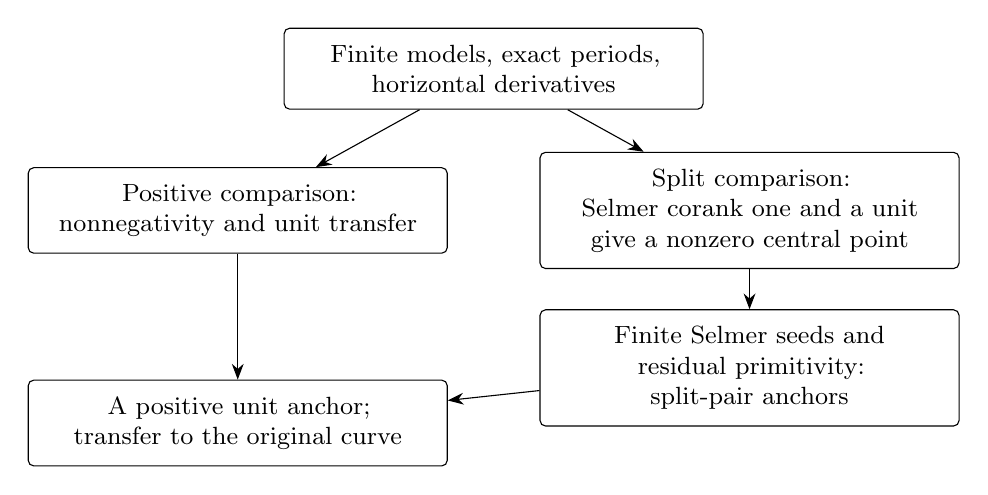
\begin{tikzpicture}[
 box/.style={draw,rounded corners=2pt,align=center,font=\small,
 text width=4.9cm,inner sep=6pt},
 >={Stealth[length=2mm]},node distance=10mm and 10mm]
 \node[box] (base) at (0,0) {Finite models, exact periods,\\horizontal derivatives};
 \node[box] (positive) at (-3.25,-1.8) {Positive comparison:\\nonnegativity and unit transfer};
 \node[box] (split) at (3.25,-1.8) {Split comparison:\\Selmer corank one and a unit\\give a nonzero central point};
 \node[box] (anchor) at (3.25,-3.8) {Finite Selmer seeds and\\residual primitivity:\\split-pair anchors};
 \node[box] (target) at (-3.25,-4.5) {A positive unit anchor;\\transfer to the original curve};
 \draw[->] (base) -- (positive);
 \draw[->] (base) -- (split);
 \draw[->] (split) -- (anchor);
 \draw[->] (positive) -- (target);
 \draw[->] (anchor) -- (target);
\end{tikzpicture}
\caption{Logical order in the non-CM proof.  Nonnegativity precedes
the anchor.  The Hecke-field rank test used by the comparators starts
with a classically known simple analytic product and does not use a
residual unit conclusion.  The direct CM argument is treated separately.}
\label{fig:logic}
\end{figure}

\paragraph{Navigation.}
Section~\ref{sec:classical} fixes the classical inputs and exact
Gross--Zagier factors; Section~\ref{sec:foundations} proves the common
cochain and determinant lemmas. Sections~\ref{sec:siegel}--\ref{sec:positive-completion}
prove Proposition~\ref{prop:positive}, with the unknown-rank
Bockstein argument in Section~\ref{subsec:positive-completion:bockstein}.
Sections~\ref{sec:split-measures}--\ref{sec:split-local} establish the
split determinant, its horizontal divisibility, and the central rank
test. The reducible anchor is completed in Section~\ref{sec:reducible}.
Section~\ref{sec:cm} proves Proposition~\ref{prop:cm} and the CM
comparison used later. After the alternation calculation in
Section~\ref{sec:alternation-imaginary}, the imaginary \(S_3\), real
\(S_3\), and cyclic-cubic anchors are proved in
Sections~\ref{alternation-imaginary:anchor-section}, \ref{sec:real},
and~\ref{sec:cyclic}, respectively. Section~\ref{sec:conclusion}
assembles these branches.

Our notation is local to each construction when a field, coefficient
ring, or modular factor changes.  Orders at height-one primes refer to
the corresponding discrete valuation rings; valuations of dyadic
constants always retain the normalization \(v_2(2)=1\).

\section{Classical facts and normalizations}\label{sec:classical}

\subsection{Analytic low-rank inputs and parity}

We use modularity of elliptic curves over \(\mathbb Q\)~\cite{BCDT01}
and the Gross--Zagier--Kolyvagin theorem: analytic order zero or one
gives the corresponding rational rank and finiteness of the whole
Tate--Shafarevich group~\cite{GZ86,Kolyvagin90}. This implication
will be applied after the analytic order has been established.

Two quadratic-twist nonvanishing results supply the auxiliary analytic
inputs. For a primitive weight-two form of trivial central character,
Friedberg--Hoffstein supplies central values with prescribed local
behavior and compatible sign~\cite{FH95}; see also
\cite[Theorem~10.6]{AnandavardhananPrasad13}. In particular, when the
base form has odd functional sign, we may choose an odd fundamental
imaginary discriminant, split at the level and at any indicated finite
additional primes, whose twist has nonzero central value. When the base
central value is nonzero, the Bump--Friedberg--Hoffstein and
Murty--Murty derivative nonvanishing results supply imaginary Heegner
twists with a simple zero~\cite{BFH90,MurtyMurty91}.

The auxiliary fields may be chosen to have only the units \(\pm1\).
For a fundamental discriminant \(b\) coprime to the level \(N\),
the twist changes the functional sign by \(\chi_b(-N)\), where
\(\chi_b\) is the associated Dirichlet character. Every local
prescription below respects this sign condition.

Finally, the modular-symbol period theorem gives rationality of central
values after division by modular periods. Their nonnegativity for
elliptic newforms follows from the positivity theorem for self-dual
symplectic forms; see \cite{LapidRallis03}.

\begin{lemma}[Two-primary parity]\label{lem:classical-parity}
For every elliptic curve \(A/\mathbb Q\),
\[
 (-1)^{s_2(A)}=w(A).
\]
For a quadratic field \(K=\mathbb Q(\sqrt{k})\),
\[
 s_2(A/K)=s_2(A)+s_2(A^k).
\]
Moreover, \(\dim_{\mathbb F_2}\Sel_2(A)-\dim_{\mathbb F_2}A(\mathbb Q)[2]-s_2(A)\) is a nonnegative even integer. These statements do not require finiteness of \(\Sha(A)\).
\end{lemma}

\begin{proof}
Kramer's quadratic-extension parity comparison~\cite{Kramer81}
and the Kramer--Tunnell local root-number/norm-index
theorem~\cite{KramerTunnell82}, including the dyadic results
of \cite{DD10,DD11,CI16}, give by the Hilbert product formula
\[
 (-1)^{s_2(A)+s_2(A^b)}=w(A)w(A^b).
\]
Parity computed by finite two-descent agrees with Selmer-corank parity
after subtracting the rational two-torsion dimension. Indeed, the
Cassels--Tate pairing modulo divisibles is alternating, since the
elliptic polarization is represented by the rational divisor
\([O]\)~\cite[Remark~I.6.11]{MilneADT}
\cite[Theorem~5 and Corollary~7]{PoonenStoll1999}.

Calibrate the displayed relative parity equality using a coprime twist
of sign plus with nonzero central value, supplied by the nonvanishing
theorem. When the sign must change, take a negative discriminant split
at the level. The analytic rank-zero theorem gives \(s_2=0\) for this
twist, so its Selmer parity equals its functional sign. The relative
equality then proves the first assertion for \(A\).

Restriction and induction give the rational decomposition over a quadratic field. The associated isogeny preserves the rational Kummer Selmer conditions, proving the displayed corank identity. Finally the same alternating pairing gives the stated even difference between finite Selmer dimension and Selmer corank.
\end{proof}

\subsection{Gross--Zagier with absolute heights}

We use the conductor-one Gross--Zagier theorem at a coprime split
level, with the normalization in
\cite[Chapter~I, (4.3) and (6.4); Chapter~V, Theorem~(2.1)]{GZ86};
see also \cite{CST14,Conrad03}. The following choices fix the trace,
polarization, and height factors needed in the determinant comparison.

Let \(f\in S_2(\Gamma_0(N))\) be the normalized primitive eigenform,
and let \(K\) have odd fundamental discriminant \(-D<-4\), prime
to \(N\), with all level primes split. Choose an oriented ideal of
norm \(N\) with cyclic quotient. Let \(P_X\in J_0(N)(K)\) be the
Hilbert-class trace of the associated maximal-order Heegner point
minus the cusp \(\infty\); the trace sums once over the class group.
Write \((f,f)_N\) for the unnormalized Petersson integral on the
ordinary \(\Gamma_0(N)\)-quotient.

Project to the rational newform orbit orthogonally on the Jacobian,
up to isogeny, and use the \emph{restricted} polarization. Since
Rosati fixes the real Hecke field, its embeddings split the resulting
height pairing. Denote the diagonal at the embedding corresponding to
\(f\) by \(H_{\rm abs,f}\). Here absolute logarithmic heights are
divided by the field degree, and the pairing uses the Poincaré
principal-pairing convention.

\begin{theorem}[Split Gross--Zagier formula]\label{thm:classical-gz}
With the preceding hypotheses and units modulo signs one,
\[
 \frac{\sqrt D}{8\pi^2(f,f)_N}\,L'(f/K,1)=2H_{\rm abs,f}(P_X).
 \tag{GZ}\label{eq:GZ}
\]
\end{theorem}
The pairing in the relative formula is over \(K\), before division
by \([K:\mathbb Q]\); this accounts for the factor two in
\eqref{eq:GZ}. The ordinary pairing on the orbit projections is the
sum of the pairings at the Hecke embeddings.

For a rational modular parametrization \(\phi:X_0(N)\to E\), put
\(\phi^*\omega_E=c_E f\,dq/q\), where
\(q=\exp(2\pi i\tau)\), and let \(P=\phi_*P_X\). Then
\[
 L'(E/K,1)=
 \frac{\int_{E(\mathbb C)}|\omega_E\wedge\bar\omega_E|}
 {\sqrt D\,c_E^2}\cdot 2 H_{\rm abs}(P).
 \tag{GZ-E}\label{eq:GZ-E}
\]
Indeed, the projection formula divides the pushed-forward pairing by
\(\deg\phi\), while pullback of the differential gives
\[
 (\deg\phi)\int_{E(\mathbb C)}|\omega_E\wedge\bar\omega_E|
       =8\pi^2c_E^2(f,f)_N.
\]
These two degree factors cancel in \eqref{eq:GZ-E}.

The absolute Poincaré-pairing diagonal is
\(H_{\rm abs}(P)=\lim_j4^{-j}h_{x,\rm abs}(2^jP)\).
The origin divisor has canonical height \(H_{\rm abs}/2\), and
the Poincaré height uses its bilinearization \emph{without} another
halving. Thus this is the height convention fixed in the introduction.
The factor two from the relative height over \(K\) remains present.

We will compare \eqref{eq:GZ-E} with the BSD arithmetic volume using
the exact Manin, Tamagawa, and full-index factors for this single
Hilbert trace. This uses the height theorem; equality with the BSD
arithmetic volume is the further assertion to be proved.

\subsection{The split discrepancy identity}

Assume now that \(L(E/K,s)\) has a simple zero at one. The classical
elliptic theorem and isogeny give finiteness of the relevant
Tate--Shafarevich groups. Apply the abelian-variety isogeny invariance
of the BSD arithmetic volume~\cite[Theorem~2.1]{Tate1966}, extending
the elliptic comparison of Cassels~\cite{Cassels65}, to
\[
 \operatorname{Res}_{K/\mathbb Q}E_K\sim E\times E^k.
\]
We compute that volume on the restriction of scalars as follows.

The Néron restriction has period
\(\int|\omega_E\wedge\bar\omega_E|/\sqrt D\).
The differential remains minimal: bad places split, and good reduction
remains good. Coordinates in an integral quadratic basis give the
dual Lie-volume lattice; its real Jacobian contributes the quadratic
discriminant. Components at bad primes contribute \(c_\ell(E)^2\).
At ramified primes of good reduction, the special restriction fiber
is connected, with a vector kernel over the good special fiber.
Finally, the points and Tate--Shafarevich group are those over \(K\),
and the principal dual height diagonal is \(2H_{\rm abs}\).

\begin{corollary}[The full-index discrepancy]\label{cor:classical-G}
Under these assumptions, the single Hilbert-class trace satisfies
\[
  X(E)+X(E^k)
  =v_2\!\left(\frac{[E(K):\mathbb ZP]^2}
      {c_E^2\,\prod_\ell c_\ell(E)^2\ \#\Sha(E/K)}\right).       \tag{G}\label{eq:G}
\]
Here \([E(K):\mathbb ZP]\) is the full group index, including torsion.
\end{corollary}

\begin{proof}
Apply \eqref{eq:GZ-E}, then divide the analytic leading term by the arithmetic volume just computed. The squared full index converts the point height to the full Mordell--Weil regulator and retains the torsion factor. Taking \(v_2\) gives \eqref{eq:G}.
\end{proof}
The quantities defining \(X\) in the allowed analytic ranks are indeed positive rationals individually: in rank one take a nonvanishing split imaginary companion and use (GZ-E) and the rational elliptic rank-zero result for the other factor (or the modular period ratios). Here equality of arithmetic volumes on restriction and the product is over \(\mathbb R\), with \emph{total} real periods. The isogeny formula likewise allows changes of the rational curve in its isogeny class, or of its twists by induced isogenies, once in these analytic ranks. The general corank condition is itself isogeny-invariant without knowing these ranks. 

\section{Finite cochain models and determinant comparisons}\label{sec:foundations}

The determinant arguments use cohomology at moving finite levels, together
with local conditions, cup products, and distinguished classes. We first
construct finite free models that retain these maps under passage to a
limit. We then prove the evaluation and determinant comparisons used to
change local conditions. The final two subsections compute the central
Kummer volumes and give the bounded-series tests needed for specialization.

We use local Tate duality and global Poitou--Tate duality, including compact
support with Tate modification at real places; see \cite{MilneADT}. The
mapping-fiber and Bockstein language is that of Selmer
complexes~\cite{Nekovar06}. At two, the standing hypotheses in that reference
impose a totally imaginary base field; our ordinary-positive and Tate-real
comparisons over \(\mathbb Q\) are given explicitly below. The other standard
inputs are étale localization and purity, Shapiro's Lemma, and arithmetic
cohomological dimension and finiteness theorems.

A global support \(S\) for a number field \(F\) includes the primes over 2
and the archimedean places; a list just of finite allowed primes leaves the
archimedean places understood. Write \(G_{F,S}\) for the
unramified-outside-\(S\) quotient. Frobenius in a coefficient action means
arithmetic Frobenius. Translating that action to a weight on a CM translate,
group polynomial, or Euler product can therefore introduce an inverse
variable; the weights in each comparison use the same convention.

For finite or compact 2-primary coefficients \(M\), \(G(M)\) and \(L_v(M)\) denote the unrestricted global and local continuous cochain complexes for the indicated support. We also write \(C_{\rm glob}(M)\) and \(C_v(M)\). A Selmer complex with local maps \(U_v\to L_v\) is
\[
 C(U,M)=\mathrm{fib}\big(G(M)\longrightarrow\bigoplus_v Q_v\big),\qquad
                Q_v=\mathrm{cone}(U_v\to L_v);
\]
we use cohomological mapping fibers (cone shifted by \(-1\)). “Strict” and “full” usually mean \(U_v=0\) and \(L_v\), respectively, at the indicated place only. “Finite” will refer to a Kummer or an unramified/Frobenius condition as specified. We omit terms imposing no condition. A separate positive complex over \(\mathbb Q\) uses the mapping fiber of restriction to \textbf{ordinary} \(C^\bullet(\mathbb R,M)\). Complex places do not contribute local conditions. By dual on coefficients we mean Tate dual (linear dual with twist (1), or compact/discrete duals as appropriate). Write \(P^\vee\) on complexes for the derived linear dual with \emph{no} shift unless specified.

\subsection{Finite models with marked arithmetic maps}

Some parameters come from a fixed tower, while others come from cyclic
extensions whose conductors move. Both are treated at finite Artin
precision. For the moving parameters, the limit is taken on the matrices
of the arithmetic diagrams; it is not cohomology of a new infinite-conductor
Galois group.

For example, a cyclic generator of order \(2^m\), written \(1+u\), gives
the relation \((1+u)^{2^m}-1\). At the fixed precision
\((2^n,u^n)\) this relation vanishes for all sufficiently large \(m\).
Thus the growing cyclic group rings have the same finite precisions as
\(\mathbb Z_2[[u]]\). The following lemma carries the cochain maps, as
well as the coefficient rings, through this passage.

\begin{lemma}[Finite models and matrix limits]\label{lem:foundations-finite} Consider diagrams of the global, local, and mapping-fiber cochain complexes above over finite local Artin coefficient rings of 2-power characteristic, with modules finite free (and compatible lifts), in systems with fixed finite residue field and only boundedly many moving places. Assume the dimensions of the residual cohomology of each complex to be modeled are uniformly bounded per degree; if a bounded perfect model is used integrally, assume these dimensions vanish outside uniformly bounded degrees as well. Then the following constructions can be made by cochain contractions.

\begin{enumerate}
\item There are degreewise finite free minimal models with ordinary base change, bounded where indicated. Continuous actions over complete rings at a stage can be treated with compatible contractions. Tensoring a model of a free coefficient also computes cochains with its tensor by any fixed finite scalar module with trivial Galois action (at compact precision, or with completed finite module).
\item Suppose on a fixed nonprincipal ultrafilter on a sequence of stages the scalar precisions identify, by reduction, with every fixed finite Artin precision of a complete local limiting ring \(R\). Here and below arbitrary such increasing precisions cofinal with powers of the maximal ideal can be used. Transfer cochain diagrams at the stages and take matrix limits at all fixed precisions. The resulting finite free models retain maps, homotopies, exact triangles (with their identifications), specified cycles and cup-product/duality diagrams when marked as below. Any fixed continuous integral parameter substitution commutes with this construction. Fixed-group diagrams whose coefficient actions already stabilize mod each precision in this identification compute the actual cohomology and maps. One can extend a previously taken diagram by further moving-prime operations on the \emph{same} stages and ultrafilter, retaining previous models and maps; one can work to a slower cofinal precision for the extensions.
\end{enumerate}

\end{lemma}

\paragraph{Arithmetic hypotheses for the models.}
The concrete limit rings for arithmetic diagrams will be power series over finite \(2\)-adic integer rings, or over a fixed finite complete local algebra, possibly after base change. The number of moving primes counts distinct places, not ramification degrees.

On global complexes the residual bounds required here, for a fixed residual representation up to a bounded filtration by fixed ones, follow by a fixed finite extension killing those representations and Kummer theory there (and Hochschild--Serre or inflation bounds and duality). For instance valuations allowed in squareclasses increase by only a bounded number of coordinates; degree two is bounded by Poitou--Tate. The local bounds use the usual local theory; degrees above two globally contribute only real cohomology and restriction to all real places there is an isomorphism. In particular positive complexes with no other conditions have the requisite bounded range, and over a totally imaginary field the ordinary global complexes do too.

\begin{proof}
\emph{Contraction at finite precision.}
Continuous cochains with free coefficients at finite precision are flat-term (filtered colimit over finite clopen partitions); reduction or tensor of the terms is ordinary cochains. Over a local Artin ring flat modules are free: lift a residue basis, use nilpotence for surjectivity and then flatness for the kernel modulo the maximal ideal followed by nilpotence again. Residually split the vector-space complex into its cohomology with zero differential and a sum of disks (a differential isomorphism with bases in adjacent degrees), and lift the graded bases. Let \(d_0\) be the pure disk differential in them, \(i,p,h\) the inclusion, projection and contraction with \(h^2=hi=ph=0,\ 1-ip=d_0h+hd_0\). For the actual \(d=d_0+\epsilon\), use
\[
 \begin{aligned}
 I&=(1+h\epsilon)^{-1}i,& P&=p(1+\epsilon h)^{-1},\\
 H&=h(1+\epsilon h)^{-1},& d_{\rm small}&=p\epsilon(1+h\epsilon)^{-1}i.
 \end{aligned}
\]
These are the disk contraction formulas (multiplication using \(d_0\epsilon+\epsilon d_0+\epsilon^2=0\) gives \(dI=I d_{\rm small}, P d=d_{\rm small}P, PI=1, dH+Hd=1-IP\)); the series are finite in the nilpotent ideal. 

\emph{Compatible diagrams.}
Bases of continuous cochains at successive quotients can be lifted compatibly by surjectivity on functions; the resulting maps of inverse limits give the same identities. Transfers of maps insert \(I,P\); compositions have the homotopies from \(H\). Analogously transfer multilinear cup maps in the required degrees by tensoring the contractions. For a mapping cone/fiber one can use the cone/fiber of a transferred map with the induced homotopy equivalences, or its minimal contraction. Acyclic reductions of cones can be retained with contracting homotopies.

\emph{Matrix limits and fixed-group comparison.}
Ranks and all finite scalar entries used in these identities have simultaneous ultrafilter values, degree by degree and compatibly by reduction; zero regions of minimal models remain zero. For fixed-group comparison at each compact scalar quotient one can compare to a further fixed contraction for the ordinary cochains at that quotient by composing inclusions and projections. On cohomology the inverse isomorphisms are between finite groups and compatible across quotients by the actual cochain reductions. The same comparisons commute with the marked maps (or one transfers the comparison homotopies on the fixed models too). Passing to compact inverse limits has no \(\lim^1\) issue, by finiteness/compactness. 

Extensions of a diagram use the old contractions on the needed old objects on ultrafilter-large sets at each precision (matrix bases can be padded or stabilized per degree). One may choose a slower single cofinal working precision on these sets. At no point does one define a new infinite-conductor profinite Galois group and posit Poitou--Tate on it.

\end{proof}

\subsection{Localization and compatible duality}

\paragraph{Change of support.}
Over a totally imaginary field the arithmetic \(S\)-integer scheme computes \(G_{F,S}\)-cohomology for our lisse systems. Indeed the 2-primary comparison is checked residually after finite covers trivializing coefficients; in the universal such cover higher cohomology of \(\mathbb F_2=\mu_2\) vanishes. Degree one is the torsor criterion, and in degree two use Picard modulo 2 and Brauer. Brauer classes die by even local degrees eventually at all of \(S_f\) in the cyclotomic tower (also at odd residue cardinalities, which have infinite order), then Picard classes by Hilbert principalization. Higher degrees vanish already over imaginary layers (use localization to the generic point and purity, cohomological dimension, and in degree three surjectivity of Brauer residues away from \(S\) by Brauer reciprocity since \(S_f\ne\varnothing\)). 

Thus allowing additional odd places where a coefficient is unramified changes the full complex by the sum of local singular quotients, i.e. local cochains modulo the inflated
\[
                         [M\xrightarrow{\mathrm{Fr}-1}M]\qquad(0,1).
\]
Inflation into the new global problem imposing just these unramified conditions there is the quasi-isomorphism (étale localization and local excision); fixed conditions elsewhere commute with it. The same works at compact precisions and limits. At unramified coefficients a singular block can be computed as the residue cochains on \(M(-1)\) shifted by \(-1\). More generally local computations at odd places discard the exact-invariants pro-(prime-to-2) kernel of inertia, then use procyclic \(2\)-inertia and residue cohomology. The inertia differential in degrees 0,1 uses generator minus one; under a power \(z\mapsto z^b\) the change on the generator cochain uses \((z^b-1)/(z-1)\) in completed procyclic notation. These are finite-model formulas (the usual two-term procyclic resolution, followed by the residue Frobenius fiber), so when the conjugating power tends to 1 the change term tends to 1 on finite precisions with pro-2 action. Unramified conditions after inverting 2 at odd places with fixed possibly ramified Tate action will be described separately.

\paragraph{Cup products and traces.}
On an imaginary base retain full global, full finite local \(L=\bigoplus L_v\) and compact \(G_c=\mathrm{fib}(G\to L)\) diagrams. Cup/invariant give a perfect pairing of \(G_c\) with the dual coefficient's unrestricted \(G'\) of shift \(-3\), and of \(L,L'\) of shift \(-2\); the connecting \(L\to G_c[1]\) is adjoint to localization, up to orientation of fibers. These are standard Poitou--Tate/local duality over the residue field, and hold over the scalar rings with free coefficient models as well. 

More explicitly transfer the cup maps, invariant and compact trace (to scalars in degrees two locally and three globally), and the reciprocity/adjunction diagram including its homotopies. The traces on scalar cochains with twist (1) can be taken at finite precision first: top cohomology is the scalar ring by the invariant or compact invariant theorem, compatibly and linearly under reduction (dually the constant degree-zero invariants of the finite dual); higher cohomology vanishes. Thus on minimal models the top degree term for each trace is one copy with zero incoming differential and the trace gives a morphism there. 

The compact map and local invariants agree on boundaries in this diagram by the ordinary compact-support triangle. The resulting cup morphisms lift residual perfectness to equivalences by the finite models. Equivalently, for the full compact/global adjunction use the cone cochain cup into compact scalar cochains, and trace; restriction on the unrestricted factor then pairs with local boundary by the local trace. These equivalences and the triangle adjunction survive the matrix limit and base changes. One may incorporate conjugate field transport in the identification of the second coefficient with a Tate dual (e.g. an anticyclotomic scalar twist); in that convention exact complementary conditions must be tested at the corresponding conjugate places.

\begin{lemma}[Complementary local conditions]\label{lem:foundations-duality}
If paired perfect local maps \(U\to L,\ U'\to L'\) (possibly only over a localized test ring after the limit) have a paired restriction nullhomotopy and induce \(L'/U'\simeq U^\vee[-2]\), the two Selmer complexes are perfect duals with shift \(-3\). \end{lemma}

\begin{proof}
Dualize \(G_c\to C(U)\to U\) and use the localization adjunction to identify the dual fiber. The comparison boundaries for nested local conditions with compatible orthogonality data are localization adjoints by the same triangles. The local equivalence can be checked on residue fields by perfectness; when the local pieces are split free in cohomology, the invariant restriction morphism is tested just in total degree two. We specify nullhomotopies or their existence from degree/amplitude or unramified factorizations when used; exact Selmer orthogonality on a DVR does not follow just from two generic dimensions.

\end{proof}

\paragraph{The real place.}
Over \(\mathbb Q\), integral calculations without a perfectness assertion for full dual pairs use ordinary positive models and finite Poitou--Tate (modified Tate at the real place in that duality). In 2-inverted comparisons the real term of the positive-complex triangle contributes just the invariant module, in degree one in the determinant of the fiber. Ordinary global complexes then have the imaginary-base comparisons above: one can first include diagrams by restriction/induction to \(\mathbb Q(i)\), whose ramification is allowed, and project by the two maps after inverting 2. Restriction/corestriction and Shapiro are cochain identities up to homotopy, transferred in the finite diagrams, so the ordinary models, even if originally unbounded at real cohomology, become perfect direct summands there. Alternatively use the splitting of induced coefficient morphisms with denominator 2. This proves the duality and unramified inflation comparisons in that setting; the averaging scalar in adjunction is invertible there. 

A different integral use over \(\mathbb Q\) is with Shapiro coefficients from a quadratic imaginary field, when ramification of that field is allowed. The modified real term of such a coefficient is contractible even integrally. The paired Shapiro cup pushed by trace to scalar cochains uses local/compact invariant \textbf{compatible with corestriction}, not twice the invariants over the imaginary base. Compact scalar cochains here use modified Tate localization at infinity. They can still be used degreewise for their degree-three trace as above (top cohomology by finite Poitou--Tate); the bounded dual pair and comparison maps for the induced coefficients equivalently identify by Shapiro. At discriminant primes newly allowed one retains the unramified Kummer/cochain conditions over the imaginary field as appropriate.

\paragraph{Character pushforward.}
Twisted classes obtained by a coefficient character map on an induced group-ring coefficient are unnormalized traces. Concretely, restricting the resulting corestriction up to a field trivializing that character gives the sum over translates with the character weights, not division by the group order. This applies at finite precisions, including when 2 is not inverted. Conversely at a fixed characteristic-zero character one may compare local conditions using its projected summand before further inverse limits if projector denominators are then bounded.

\subsection{Evaluations and Frobenius tests}

\begin{lemma}[Detection by evaluations]\label{lem:foundations-evaluation}
For the limiting unrestricted global \(H^1\), after scalar specialization even to height-one residue fields, there is an injection by evaluations into abstract crossed homomorphism classes on \(\mathcal G_F=\prod_i G_F\), where \(i\) runs over the stages. The action on a fixed-rank module is given by entrywise ultrafilter limits before specialization. \end{lemma}

\begin{proof}
Retain the model inclusions into the actual global cochains. Evaluations
on every sequence of group elements, pairs of sequences, and higher tuples
have simultaneous matrix limits. They preserve the cochain equations, so
degree-one cycles give crossed homomorphisms on \(\mathcal G_F\).

It remains to show that evaluation detects their cohomology classes after
specialization. At each residual stage a bounded finite list of group
elements detects invariants and whether a model cocycle is a single
coboundary. These are linear equations on bounded-dimensional spaces.
The resulting evaluation map to
\[
                         E=[M\longrightarrow M^{\rm list}]
                         \qquad\text{in degrees }0,1
\]
is therefore an isomorphism on residual \(H^0\) and injective on residual
\(H^1\). For its unshifted mapping cone \(K\), writing \(k\) for the
residue field, the long exact sequence gives
\[
                         H^{-1}(K\otimes k)=H^0(K\otimes k)=0.
\]
The complexes start in degree zero, so a degreewise minimal model of
\(K\) has no terms in degrees at most zero. This remains true after every
field base change. The same long exact sequence now proves the required
\(H^1\)-injection at the specialized field. No upper boundedness of the
ordinary real cochains is needed for this low-degree argument.

Conjugation and comparison identities on evaluations hold on classes by
the transferred homotopies. A Selmer \(H^1\) likewise injects whenever its
local maps include full \(H^0\) and inject in \(H^1\) at the field being
tested.
\end{proof}

\paragraph{Detection on a kernel.}
Let \(\mathcal H\) be a normal joint kernel acting trivially on the
coefficients. Restriction to \(\mathcal H\) gives additive, equivariant
evaluations. Inflation--restriction shows that these detect classes if
\(H^1(\mathcal G_F/\mathcal H,M)=0\). One sufficient condition is a central
scalar whose difference from one is invertible, by the crossed-homomorphism
identity.

\paragraph{The open-image criterion.}
A second criterion applies in characteristic zero. Suppose the quotient
contains, as a normal subgroup, the product
\[
                   \mathcal S=\prod_i\mathrm{SL}_2^b(\mathbb Z_2)
\]
of a fixed deep principal congruence subgroup, acting on the standard
plane by the limiting matrices, with all scalar twists trivial on
\(\mathcal S\). Then
\[
                         H^0(\mathcal S,M)=H^1(\mathcal S,M)=0,
\]
where \(H^1\) denotes even abstract group cohomology. These vanishings imply
the required vanishing on the quotient.

To prove them, choose the constant diagonal
\(D=\operatorname{diag}(m,m^{-1})\), with an integer \(m>1\) sufficiently
close to one. The matrix \(D-1\) is invertible. Adjust a cocycle to vanish
at \(D\); commutation with \(D\) then makes it vanish on every sequence
of diagonal elements. For an upper-unipotent sequence \(U\), conjugation
by \(D\) gives the integer power \(U^{m^2}\). The crossed identity gives
\[
             \left(D-\sum_{j=0}^{m^2-1}U^j\right)x(U)=0.
\]
This triangular matrix is invertible: its diagonal entries are
\(m-m^2\) and \(m^{-1}-m^2\). Using \(D^{-1}\) gives the same conclusion
for lower unipotents. Gaussian factorization into lower-unipotent,
diagonal, and upper-unipotent factors works termwise inside the same
principal congruence subgroup. Hence it works for arbitrary sequences,
and the cocycle vanishes on \(\mathcal S\).

This subgroup is available for an open elliptic Tate image when the
competing data have uniformly bounded derived length over a fixed finite
field extension. A sufficiently iterated closed derived subgroup kills
those data and contains a deep \(\mathrm{SL}_2\) in the Tate image, by
Lie brackets first in the open matrix group and then in
\(\mathfrak{sl}_2\). The depth can be chosen uniformly at the stages.

\paragraph{Joint evaluations and Frobenius selection.}
On a simple coefficient space with scalar endomorphisms, the joint evaluations of linearly independent classes detected by that restriction span a full tuple space. A proper span, by equivariance and semisimplicity of a sum of copies of the simple, would impose a scalar linear relation. In characteristic zero additive evaluations then permit simultaneous nonidentically-zero polynomial tests (integer combinations). Even in characteristic two, if full span gives rank two somewhere for a \emph{linear} pair-coordinate test, additivity gives rank two on the kernel evaluations: a homogeneous quadratic vanishing on an additive subgroup vanishes on its field span by polarization. 

Finally by Chebotarev a Frobenius sequence can agree with a selected sequence of elements on all old evaluation matrices and other designated finite continuous data to increasing precision: continuous functions at each Artin precision factor through finite sets on finite quotients, and one uses a chosen representative over the prime. In inert-prime tests of squares one uses the desired coset and takes normal closures of the bounded-precision data over the base. Additional splitting and determinant prescriptions will need actual compatibility, which will be checked in each use. This procedure preserves old evaluations when enlarging support (with unramified initial condition at a new place via the localization comparisons).

\subsection{Determinant volumes and complementary changes}

We use the determinant-line formalism for perfect complexes
\cite{KnudsenMumford76}, with the inverse convention specified below.
The complementary-condition switches are related to finite--singular
comparisons in \cite[Section~1.2]{MazurRubin04}; the following proofs
retain their exact local determinant volumes.

Use the line
\[
 \mathcal D(C)=\bigotimes_i(\det C^i)^{(-1)^{i+1}}
\]
for a perfect complex (the inverse of the cohomological determinant), and its canonical exact-triangle and cohomology identifications, ignoring harmless determinant signs. For a DVR with valuation \(v\), \(d(C,x)\) is the valuation of the coefficient of a generic tensor \(x\) relative to a generator of \(\mathcal D(C)\); an infinite value is allowed for zero. A torsion elementary divisor in cohomological degree \(i\) of length \(b\) contributes \((-1)^{i+1}b\), in uniformizer units of value one, to \(d\) on free cohomology bases. For a square \([F\xrightarrow{\delta}G]\) in degrees 1,2 with finite-length cohomology, \(d(C,1)=-v(\det\delta)\). These statements follow immediately by splitting into elementary-divisor blocks. For a self-duality of shift \(-3\) pairing degrees 1 and 2 of rank one generically, \((Y,Y^\vee)\) will denote the determinant tensor of a degree-one class \(Y\) with its pairing functional on degree two.

\begin{lemma}[The strict--finite determinant comparison]\label{lem:foundations-D}
Comparisons of local conditions \(U\subset V\) give a triangle \(C(U)\to C(V)\to V/U\). Suppose at a split pair of places one complex \(C_*\) uses strict at \(w\), full at \(\bar w\); \(C_F\) uses exact orthogonal \(U_w,U_{\bar w}\), keeping other exact orthogonal conditions, with conjugate duality (so \(Q_{\bar w}\simeq U_w^\vee[-2]\)). Assume perfect comparisons including duals over our DVR, and generic \(U_w\) a line in degree one only. Write \(C_0\) for strict at \(w\), \(U_{\bar w}\) at \(\bar w\). We have
\[
 C_0\to C_F\to U_w,\qquad C_0\to C_*\to Q_{\bar w}.
\]
Over the fraction field suppose \(C_*\) acyclic and a class \(Y\in H^1(C_F)\) has nonzero localization in \(H^1(U_w)\). The triangles show \(C_F\) has only a line in each of degrees 1,2 and degree one maps isomorphically onto that localization line. Conversely these line assertions force strict acyclicity (using duality: the boundary from \(Q_{\bar w}\) is then nonzero by adjunction). Write \(\operatorname{loc}_wY=p e\) for a fraction-field basis \(e\). Exactly
\[
 d(C_F,(Y,Y^\vee))=d(C_*,1)+2\big(v(p)+d(U_w,e)\big).       \tag{D}\label{eq:D}
\]
\end{lemma}

\begin{proof}
For \(x=\partial(e^*)\in H^2(C_0)\) by the second triangle, \(x\) pairs after projection with \(Y\) by \(p\), by the same adjunction. Thus up to signs the two tensors compared via \(C_0\) give \(p^2 x^*\otimes e,\ x^*\otimes e^*\), respectively; the two local lattice volumes are dual. The computation works also for rationally imposed local conditions in compatible triangle volumes defined by assigning a DVR determinant lattice on \(U_w\) and the dual one on \(Q_{\bar w}\).

\end{proof}

\subsection{Line and square switches}

A switch changes the condition at one newly allowed place. Fix nested
local conditions \(U_-\subset U_+\), and intermediate conditions
\(U_f,U_s\) whose quotients over \(U_-\) give a direct-sum decomposition
of \(U_+/U_-\). Over the test DVR, assume these two quotients are free
and concentrated in degree one. Their coordinates are called finite
and transverse (pure singular), and denoted \(f,s\). Let
\(C_-,C_+,C_f,C_s\) be the four resulting global complexes.
The local conditions form the diagram
\[
\begin{tikzpicture}[baseline=(lower.base),>=Stealth,node distance=8mm and 16mm]
\node (lower) {\(U_-\)};
\node (finite) [above right=of lower] {\(U_f\)};
\node (singular) [below right=of lower] {\(U_s\)};
\node (upper) [below right=of finite] {\(U_+\)};
\draw[->] (lower) -- (finite);
\draw[->] (lower) -- (singular);
\draw[->] (finite) -- (upper);
\draw[->] (singular) -- (upper);
\end{tikzpicture}
\qquad
 U_+/U_-\simeq(U_f/U_-)\oplus(U_s/U_-).
\]

We assume complementary dualities: the upper problem is dual to the
lower problem for the dual coefficient, and conversely. The local
pairing is perfect between the two coordinate spaces, and each pure
condition is self-annihilating against its corresponding condition on
the dual side. The global complexes have amplitude \(1,2\) over the
generic field and each indicated fiber field. The local splitting and
complementary duality hypotheses hold at both fields; the lemmas distinguish
the further generic and fiber dimension assumptions.

In the applications, the lower condition contains all local \(H^0\),
and the upper condition contains both degree-one coordinates but no
local \(H^2\). Thus the lower condition is generally not the zero
complex. Keeping this degree-zero term is what makes the changed global
\(H^1\) inject into unrestricted cohomology.

\begin{lemma}[Line switch]\label{lem:foundations-line}
Assume that the local quotient ranks are \(1,1\). Suppose \(C_f\) has just one generic cohomology line in degree one. At the fiber, if \(h=\dim H^1(C_f)>1\), arrange nonzero finite evaluations for both a primitive fiber reduction of that generic line and some degree-one class for the old dual condition. Then the switch lowers the fiber dimension from \(h\) to \(h-1\), and \(C_s\) again has a single generic cohomology line in degree one. If \(Y,Y'\) are classes for the finite and transverse conditions and \(s(Y')=f(Y)\) under an isomorphism of the two local lines of unit determinant volume, then
\[
 d(C_f,Y)=d(C_s,Y').
\]
If successive switches carry integral classes to a fiber of dimension one, this common coordinate has nonnegative valuation.
\end{lemma}

\begin{proof}
Then the generic finite evaluation is nonzero and \(C_-\) generically acyclic. On the fiber no transverse contribution can enter (it must annihilate the nonzero finite opposite evaluation by reciprocity), so \(H^1(C_s)\) has dimension \(h-1\) there by the triangles. Generically the triangle from lower gives again a line in \(C_s\), evaluating isomorphically on the local singular line.

If classes \(Y,Y'\) in \(C_f,C_s\) have \(s(Y')\) equal to \(f(Y)\) via a unit-volume line isomorphism, then
\[
                          d(C_f,Y)=d(C_s,Y')
\]
by the two triangles from \(C_-\) (same tensor 1 there). Extra unchanged terms with a fixed trivialization need not be included in this notation.

Thus in a sequence of such switches with integral classes at the test DVR and nonzero generic evaluations, when \(h=1\) the coordinate is integral (the complex is then just a free line by the minimal fiber model), and gives nonnegativity also backwards.
\end{proof}

\begin{lemma}[Square switch]\label{lem:foundations-square}
Assume that the local quotient ranks are \(2,2\), in the self-dual global setting with exact lower/upper duality. The localization image for upper in the four coordinates is self-annihilating: its annihilator is the kernel of the boundary into \(H^2(C_-)\), by adjunction, hence is the same image. Suppose \(C_f\) has generic rank one in degree one with a class \(Y\) and nonzero \(f(Y)=v_0\); then \(H^1(C_-)\) there vanishes. Suppose \(Y'\) for \(C_s\) has \(s(Y')=J v_0\) up to a unit, where \(J\) is an integral involution on a common coordinate plane, and the cross pairing of either plane with the other is \(\langle x,Jy\rangle\) up to a unit using a unimodular alternating plane form (interchanging the variables or transporting by \(J\) gives the same condition up to units). Then \(Y,Y'\) are a generic basis in upper by the half-dimension assertion, \(C_s\) has again generic rank one in degrees 1 and 2, and
\[
                    d(C_f,(Y,Y^\vee))=d(C_s,(Y',(Y')^\vee)).
\]
If the finite evaluation has rank two at a surplus-dimension fiber and is nonzero on the primitive generic class, the switch lowers the fiber dimension by two. A sequence ending at dimension one gives a nonnegative determinant valuation whenever the classes and exact self-dualities are integral at the test DVR.
\end{lemma}

\begin{proof}
We have \(H^2(C_-)=k_{\rm gen}Y^*\oplus k_{\rm gen}(Y')^*\) using upper/lower duality over the fraction field \(k_{\rm gen}\). The finite coordinate boundary pairs to zero against \(Y\); take a complement \(x\) of \(v_0\) mapping to \((Y')^*\). Then \(v_0\wedge x\) has unit plane volume by the cross pairing and the local identity. Likewise on the transverse plane interchanging the two classes. Thus the two triangles compare the class-functional tensors to the same lower tensor \((Y^*\wedge (Y')^*)^*\) times unit plane volumes. 

This comparison requires compatible duality adjunctions, as in the preceding diagram discussion. At a split-in-cohomology switch place with conditions in degrees 0,1 they may be used simultaneously: isotropic restrictions admit compatible nullhomotopies on the lower comparisons (there is no ambiguity of a morphism into scalars in degree three on those tensor products). Unchanged local conditions retain the same choices. The comparison also permits volume changes from disjoint rational local modifications when these are defined by compatible triangles.

If at a surplus-dimension fiber one arranges rank two on the old finite plane (including a nonzero evaluation of the primitive reduction), the upper localization image there is the finite plane itself. Thus the switch drops \(h=\dim H^1(C_f)\) by two, while generically the two classes give the determinant comparison just stated. 

Iteration to \(h=1\) gives nonnegative valuation for the class-functional tensor over the DVR if exact self-duality and integral classes hold there: at that fiber minimality and generic dimensions give two free lines with zero differential, paired integrally perfectly. In these switches a primitive reduction exists in a two-term DVR model before switching whenever there is a generic line: its kernel is saturated and reduction gives a nonzero fiber class.

\end{proof}

\paragraph{The local switch coordinates.}
The cross calculations will use, for example, tame evaluations at inert auxiliary primes whose residue cardinalities over a quadratic field tend to 1, with trivial local action to increasing precision. Degree one then splits by evaluation on a residue Frobenius lift and a tame generator, using the inertia/residue cochains; the two axes are isotropic for a trivial-limit scalar cup. For the inertia square cup one can retain enough roots-of-unity precision: the pure-inertia additive character at any fixed precision (Frobenius value zero) factors through cyclic inertia of much greater 2-power order since the Frobenius conjugating power is 1 to that greater precision. The cyclic scalar \(H^2\) products inflate to zero there. The mixed scalar cup is a unit with dual local bases. Conjugate transport via an inert rational Frobenius preserves axes using its square as residue lift, multiplying the inertia-generator argument by a unit; thus inserts its Tate transport on the other plane. We give the action hypotheses where applying this. 

A related pure field parity computation is for two Lagrangian conditions whose sum modulo intersection is a symmetric split plane in degree one (characteristic zero). The same upper/lower adjunction makes the upper image a self-annihilating line there, necessarily one of the two axes; switching between them thus changes \(\dim H^1\) by one in parity.

\subsection{Central Kummer lattices and local measures}

\paragraph{Kummer conditions and their duality.}
At a finite place \(v\), for an elliptic curve with coefficient \(T=T_2E\), use the local complex \(U_v=E(F_v)^\wedge_2[-1]\) when imposing the full integral ordinary Kummer condition. It maps to \(L_v\) by the Kummer map and lower truncation (integral \(H^0(F_v,T)=0\)). Its derived reductions have image all \(E[2^n](F_v)\) in degree zero and exact finite Kummer in degree one, injectively: this follows by ordinary Kummer and the Bockstein on torsion invariants, taking them to their integral Kummer classes. 

These are exact orthogonal complexes under local duality. The cup restriction is nullhomotopic over \(\mathbb Z_2\) (morphisms from the derived Kummer tensor to scalars in degree two are detected on its \(H^2\), and the Kummer pairings vanish modulo all \(2^n\)). After a nullhomotopy the local quotient duality map is an equivalence, checked by finite Kummer orthogonality and the invariants and their duals at the residue field. 

On compact cohomology the familiar sequence reads
\[
 0\longrightarrow E(F_v)^\wedge_2\longrightarrow H^1(F_v,T)
           \longrightarrow\operatorname{Hom}(E^\vee(F_v)^\wedge_2,\mathbb Z_2)
                      \longrightarrow0,
\]
by finite duality. Thus at odd finite places the compact \(H^1\) is entirely Kummer (as also at real places by the ordinary Kummer sequence, since Weil--Châtelet there has exponent two). 

The singular free coordinate at a rational dyadic place after inverting 2 uses Bloch--Kato local duality and its abelian variety comparison~\cite[Sections~3.7--3.11]{BlochKato90}: finite Kummer is the log line, and cup against it on the Tate dual is evaluation of \(\exp^*\) against the Kummer logarithm. Thus for \(\exp^*z=\alpha\omega_E\) at \(\mathbb Q_2\) the invariant against a Kummer class \(x\) is \(\pm\alpha\log_{\omega_E}x\). More generally use the differential/tangent and trace pairing. This is a rational comparison at the local prime, not a claim that \(\alpha\) is an integral quotient generator.

\begin{lemma}[The global Kummer volume]\label{lem:foundations-kummer}
For the actual all-finite Kummer complex \(C_{\rm Kum}\) over an imaginary quadratic \(K\), with enough support, derived base change to finite coefficients gives the usual Selmer in degree one by these assertions, and likewise passage to divisible coefficients. If \(\Sha(E/K)\) is finite, degree one integrally is the compact Mordell--Weil module, degree-two torsion has length \(s_K=v_2(\#\Sha(E/K))\) (the residual finite quotient in the change to \(\mathbb Q_2/\mathbb Z_2\)), and degree-three torsion has length \(\tau_g=v_2(\#E(K)_{\rm tors})\) by self-duality. The free parts in degrees one and two pair unimodularly. Thus for rank one, with \(n_P\) the index valuation on the free line of a global point \(P\),
\[
               d(C_{\rm Kum},(P,P^\vee))=2n_P+2\tau_g-s_K.          \tag{Kum}\label{eq:Kum}
\]
These valuations also use conjugate-field duality if indicated (the self-duality remains integral).
\end{lemma}

\begin{proof}
The Kummer and duality descriptions above give torsion lengths \(\tau_g,s_K,\tau_g\) in degrees one, two, and three. Their signed sum in the inverse determinant convention is \(2\tau_g-s_K\). The free point and its pairing functional each contribute its index valuation \(n_P\). This gives \eqref{eq:Kum}.
\end{proof}

\paragraph{Local measure factors.}
Write \(P_\ell(1)=L_\ell(E,1)^{-1}\). For a rational minimal differential at finite primes put \(\tau_\ell=v_2(\#E(\mathbb Q_\ell)[2^\infty])\) and \(\log_{\omega_E}E(\mathbb Q_2)=2^l\mathbb Z_2\). Haar measures give
\[
 \tau_\ell=v_2(c_\ell P_\ell(1))\quad(\ell\ne2),\qquad
 \tau_2-l=v_2(c_2 P_2(1)).
\]
Indeed the connected-point measure is the nonsingular residue size divided by \(\ell\) (the small kernel from the formal group), giving \(P_\ell(1)\); at 2 use the formal-log lattice with torsion kernel. 

At \(\mathbb R\), \(H^1(\mathbb R,T)=E(\mathbb R)^\wedge_2\) records the component factor, and a primitive Betti invariant cycle \(a\) has absolute period \(\Omega_0\) equal to the connected period, so that \(\Omega_E=\#\pi_0 E(\mathbb R)\cdot\Omega_0\).

\subsection{Bounded-series specialization and division tests}

We record four specialization principles used with these volumes. All series in these principles are bounded: their coefficients lie in a fixed complete DVR, or in its fraction field with one common denominator. This condition is stronger than belonging to the unrestricted formal series ring over the fraction field.

\begin{remark}[Specialization of determinant coordinates]\label{rem:foundations-pivots}
If a generic determinant coordinate is defined by concentration in given degrees (in particular a free degree-one cohomology determinant), at a prime where the corresponding field dimensions are the same, Gaussian pivot comparison/minimality over the local ring permits specializing the coordinate identity, even if a previous set of rational pivots vanished. In stage comparisons one may keep the pivot minors nonzero by convergence to a \emph{fixed} finite specialization, and if the resulting ranks agree, numerator, denominator and class coordinates converge by their matrix formulas. Conversely bounded torsion-length and rank tests at scalar specializations (DVR constants) keep pivots of the corresponding size nonzero in the limit.
\end{remark}

\begin{remark}[Scalar limits of measures]\label{rem:foundations-measures}
Measures can have coefficients in \(\mathcal V=W(\overline{\mathbb F}_2)\) and the constant limits can then be taken in \(\mathcal V^*=\varprojlim_n\prod_{\mathscr U}(\mathcal V/2^n)\) for the fixed ultrafilter \(\mathscr U\). This is still a complete integer DVR (nonzero elements have a finite first nonzero precision and divide uniquely by that many uniformizer factors to units). Fixed finite extensions can be embedded and used similarly with their ramification. Uniformly bounded denominators disappear after inverting 2 there. Bounded group-ring values at cyclic orders tending to infinite 2-power depth give bounded power series by reduction, \(1+u\) being a chosen generator variable. Substituting a fixed finite character (with scalar enlargement), or passing to a fixed finite group quotient, commutes with these limits. Arithmetic model matrices themselves use the smaller compact rings before further base change.
\end{remark}

\begin{lemma}[Tame division from character tests]\label{lem:foundations-series}
In a DVR-integer bounded power-series ring in \(t,\mathbf u\), a divisor \(L\) with nonzero reduction at uniformizer \(=t=0\) becomes distinguished up to a unit in one tame variable after a tame group-power coordinate change. The change may retain any fixed finite list of characteristic-zero generic ranks and nonvanishings at \(t=0\). If a bounded series \(B\) is divisible by \(L\) after inverting two at every sufficiently high two-power character in \(t\), then \(L\mid B\) integrally.
\end{lemma}

\begin{proof}
Specialize a line \(1+u_j=(1+x)^{n_j}\), one \(n_j=1\) and others successively very highly 2-divisible to separate a lexicographically leading monomial on reduction (assign the dominant lex coordinates largest \(2^{v_2(n_j)}\) in its weighted order, large relative to the lower-coordinate orders of the chosen monomial). This works simultaneously for a finite list by using the product. The line extends to a coordinate change. To retain the indicated characteristic-zero generic ranks and nonvanishings at \(t=0\), in formal log coordinates use leading homogeneous polynomials, choosing the free integers \(n_j\) avoiding finitely many proper conditions compatibly with the prescribed valuations. The same regularity test applies over a finite local coefficient order by its closed-point reduction. If a bounded \(B\) is divisible by \(L\) after inverting 2 at every sufficiently high \(2\)-power character in \(t\), then Weierstrass division in that tame variable proves \(L\mid B\) integrally. At those specializations the divisor remains regular of the same degree (evaluation always means the parameter is generator value minus one); the monic polynomial quotient has no 2-torsion, so the integral remainder vanishes there. Its bounded coefficients vanish identically by one-variable Weierstrass. One may check vanishing componentwise where the coefficient order embeds in a product of DVRs preserving the residual regularity. In general bounded nonzero series conditions in several variables can be avoided by finite-order tests by iterating the one-variable assertion (also with remaining unspecialized variables). For a nonzero bounded one-variable series the valuation at high 2-power characters is eventually the minimum coefficient valuation plus the first degree attaining it times the valuation of the parameter, by unique dominance.
\end{proof}

\begin{lemma}[The pole test]\label{lem:foundations-poles}
Let \(\mathcal O\) be a complete dyadic integer DVR. Suppose
\(f_i,g_i\in\mathcal O[[t]]\) converge coefficientwise along the fixed
ultrafilter to \(f,g\in\mathcal O[[t]]\), with \(f\ne0\). Assume, on a
filter-large set of stages, that \(f_i\ne0\) and
\[
                         g_i/f_i\in\mathcal O[[t]][1/2].
\]
No uniform bound on the denominators of these quotients is required.
Every zero of \(f\) in the open unit disk, taken in an algebraic closure
of \(\operatorname{Frac}\mathcal O\), is a zero of \(g\) with at least
the same multiplicity.
\end{lemma}

\begin{proof}
The common integral coefficient bound makes coefficientwise convergence
uniform on every smaller closed disk. Let \(\alpha\) be a zero of \(f\)
of multiplicity \(m\), and pass to a finite scalar extension containing
\(\alpha\). If \(g=0\), there is nothing to prove. Otherwise choose,
after a further finite extension if needed, a sufficiently small closed
disk about \(\alpha\) containing no
other zero of \(f\) or \(g\), and with neither series vanishing on its
boundary. After translation and rescaling, the dominant coefficient
computes the Weierstrass degree on that disk. Uniform convergence
preserves this degree for both series on a filter-large set. Thus \(f_i\)
has exactly \(m\) zeros there, while the number of zeros of \(g_i\) equals
the multiplicity of \(g\) at \(\alpha\). Stage divisibility forces the
latter number to be at least \(m\), proving the assertion.
\end{proof}

We apply this lemma after fixing the tame characters. If a denominator
factor is distinguished in \(t\), all its zeros lie in the open unit
disk. The lemma therefore makes the integral division remainder by each
required power of that factor vanish at every admissible tame-character
test. When the tests exclude only finitely many nonidentical vanishing
conditions, the bounded-series uniqueness argument above makes the
remainder vanish identically.

\section{A Siegel-unit period and lattice calculation}\label{sec:siegel}

This section constructs the integral smoothed classes used in the positive
comparison and determines their periods.  The three ingredients have distinct
roles.  A quotient that kills cusp differences gives a full integral
modular-symbol lattice.  Siegel-unit distributions give integral classes and
trace maps.  Explicit reciprocity and an archimedean calculation determine
their rational differential coordinates, including every smoothing and Euler
factor.  The integral divisibility of the normalized determinant will be
proved in the subsequent sections.

\subsection{The elliptic quotient and its relative lattice}

Fix an elliptic modular isogeny class of conductor \(N\), with normalized
newform \(f\).  Let \(E_0\) be the elliptic optimal quotient of \(J_1(N)\), so
that the quotient map has connected kernel.  Let \(C_{\mathrm{cusp}}\) be the
subgroup of \(E_0(\overline{\mathbb Q})\) generated by the images of all
geometric cusp differences, and put
\[
                         E'=E_0/C_{\mathrm{cusp}}.
\]
Manin--Drinfeld makes \(C_{\mathrm{cusp}}\) finite, and its Galois stability
makes this a \(\mathbb Q\)-isogeny \cite{ManinDrinfeld}.  If \(D_N\) is the cusp
set, the Abel map followed by this quotient gives
\[
                  \pi:(X_1(N),D_N)\longrightarrow(E',O)
\]
over \(\mathbb Q\).  Changing the base cusp changes the Abel map by a cusp
difference, so the resulting map is independent of that choice.

Allow \(A=1\) or \(A=2^k\), put \(L=NA\), and let
\[
                  \Pi:(X_1(L),D_L)\longrightarrow(E',O)
\]
be the \(A\)-degeneracy followed by \(\pi\).  The degeneracy quotients by the
cyclic subgroup of order \(A\) in the marking and pushes the marked point
forward.  At the mark \(1/L\), it is \(\tau\mapsto A\tau\).  Thus, for a
nonzero rational invariant differential \(\omega\) on \(E'\),
\[
 \Pi^*\omega=c_F F\,\frac{dq}{q},
 \qquad F(\tau)=A f(A\tau),\qquad q=e^{2\pi i\tau},
 \qquad c_F\in\mathbb R^\times.
\]
The form \(f\) has rational coefficients and trivial character and is pulled
back from \(X_0(N)\).  The marked levels are fine: weight-two cuspidality on
\(X_0(N)\) in particular gives \(N\geq5\).

Write
\[
 \Lambda_B=H_1(E'(\mathbb C),\mathbb Z),\qquad
 T=H^1(\overline E',\mathbb Z_2)(1).
\]
The principal pairing identifies
\(T=T_2(E')^\vee(1)\) with \(T_2E'\).  Choose a generator \(a\) of the
real-invariant sublattice of \(\Lambda_B\), oriented so that
\(\int_a\omega=\Omega_0>0\).  This is the connected real period.  The cycle
\(a\) is primitive and, under the comparison identifications, gives a basis
of \(T^{G_{\mathbb R}}\).  For \(\xi\in\mathrm{SL}_2(\mathbb Z)\), let
\(\delta_\xi\in H^1(E'(\mathbb C),\mathbb Z)\) be Poincaré dual to
\(\Pi_*\xi\{0,\infty\}\), with orientation fixed by
\[
       \int_{E'(\mathbb C)}\omega\wedge\delta_\xi
           =\int_{\Pi_*\xi\{0,\infty\}}\omega.
\]

\begin{lemma}[The integral relative lattice]\label{lem:siegel-lattice}
There is an integral Galois-equivariant map
\[
 H^1(\overline{Y_1(L)},\mathbb Z_2)(1)\longrightarrow T
\]
dual to pullback on relative cohomology.  When \(A=1\), there are finitely
many integers \(n_\xi\) such that
\[
              \delta=\sum_\xi n_\xi\delta_\xi,\qquad \delta(a)=1.
\]
\end{lemma}

\begin{proof}
Pullback by the map of pairs \(\Pi\) is integral.  Relative Poincaré duality
gives the displayed map; no rational Hecke projector is involved.  Its
differential coordinate for the dual exponential, with the Tate-twist
de Rham comparison, is paired by the cup invariant with the ordinary finite
Kummer logarithm on \(E'\).

For the lattice assertion, write \(E_0(\mathbb C)=\mathbb C/\Lambda_0\).
Connectedness of the kernel of \(J_1(N)\to E_0\) makes the map on integral
first homology onto \(\Lambda_0\).  The quotient by \(C_{\mathrm{cusp}}\)
replaces \(\Lambda_0\) by the lattice \(\Lambda_B\) generated by
\(\Lambda_0\) and lifts of the cusp images.  Relative cusp paths supply
exactly these additional generators.  Hence
\[
 H_1(X_1(N)(\mathbb C),D_N;\mathbb Z)\longrightarrow\Lambda_B
\]
is surjective.  The Farey triangulation generates the relative group by
Manin edges \(\xi\{0,\infty\}\).  Their images therefore generate
\(\Lambda_B\) integrally.

The invariant sublattice is the kernel of complex conjugation minus one
on a free integral lattice and is saturated; its generator \(a\) is
primitive.  Unimodularity of the intersection pairing on \(\Lambda_B\)
then makes evaluation on \(a\) surjective on \(H^1(E'(\mathbb C),\mathbb Z)\).
An integral combination of the Poincaré duals of the Manin edges consequently
has evaluation one.
\end{proof}

\subsection{Level patterns and integral smoothed classes}

We use the following two patterns of orders.  The dyadic valuation of \(M\)
will always be sufficiently large; for example, \(v_2(M)\geq6\) suffices for
the reciprocity calculation below.

\begin{enumerate}[label=(\roman*)]
\item In \emph{square order}, \(n_1=n_2=M\), with \(L\mid M\).  Set
\(l=e_2\xi\), where \(e_2=(0,1)\).
\item In \emph{rectangular order}, \(n_1=M\), \(n_2=bM\), where
\(b=N_{\mathrm{odd}}\), \((b,M)=1\), and \(2^{v_2(L)}\mid M\).  Set
\(l=(Ns,1)=e_2\xi\).  When filling the first row, also allow
\(n_1=b_1M\), where \(b_1\mid b\) is a product of some of the full prime
powers dividing \(b\).
\end{enumerate}

On \(Y(n_1,n_2)\), let \(P,Q\) be the independent marked points of the
indicated orders on the universal elliptic curve.  Independence means that
they define an embedding of the indicated product of cyclic groups.
The mark and determinant used for projection are
\[
 C=l_1(n_1/L)P+l_2(n_2/L)Q,\qquad
 \eta_M=e_M\bigl((n_1/M)P,(n_2/M)Q\bigr).
\]
Both coefficients in \(C\) are integers, including in the rectangular
case, and \(C\) has order \(L\).  The determinant \(\eta_M\) is a primitive
\(M\)-th root of unity.  Fix compatible primitive roots in algebraic,
dyadic, and complex embeddings, using \(e^{2\pi i/m}\) in the complex
embedding.

Trace to
\(Y_1(L)\times\operatorname{Spec}\mathbb Q(\mu_M)\), and then use
Lemma~\ref{lem:siegel-lattice}.  For a finite character
\(\nu\) of \(\operatorname{Gal}(\mathbb Q(\mu_M)/\mathbb Q)\), the summand
whose root is \(\zeta_M^\sigma\) receives weight \(\nu(\sigma)\).
This is an unnormalized trace: equivalently, take the group-coefficient
trace and send its basis vector at \(\sigma\) to \(\nu(\sigma)\).
For period calculations, trivialize the finite twist after restriction
using the specified embeddings.  Reversing the Galois convention replaces
the argument character consistently by its inverse.

Choose \(c,d>1\) prime to \(6n_2\).  On the variable elliptic curve \(E\),
write
\[
                {}_c g_P=P^*{}_c\theta_E,\qquad
                {}_d g_Q=Q^*{}_d\theta_E
\]
for the canonical smoothed Siegel units.  The divisor of
\({}_c\theta_E\) is \(c^2(0)-E[c]\); its norm under \([s]\) is itself
when \((s,c)=1\).  These are the normalized distributions of
\cite{Kato04}.  Norm compatibility under an isogeny of degree prime to
\(c\) follows from the divisor and uniqueness of this normalization:
the norms under \([2]\) and \([3]\) commute with the isogeny.  The Tate
formula in the proof below also checks the normalization directly.

At stage \(j\), replace the orders by \(2^j n_1,2^j n_2\) and let \(P',Q'\)
map to \(P,Q\) under multiplication by \(2^j\).  Before the mark and
determinant projection, the class is the edge image of the unnormalized
trace, at precision \(2^j\), of
\[
  ({}_c g_{P'})\cup({}_d g_{Q'})\ \otimes\
           e_{2^j}(n_1P',n_2Q')^\vee .                   \tag{K1}\label{eq:K1}
\]
Parentheses denote Kummer classes.  The dual basis sends the displayed
primitive root to \(1\), so the total coefficient is
\(\mathbb Z/2^j(1)\).

\begin{proposition}[Integral classes and dyadic compatibility]
\label{prop:siegel-integral}
The classes obtained from \eqref{eq:K1} are integral for support containing
the primes of \(2n_2\) and infinity.  They are compatible with the dyadic
division traces and, after the mark and determinant projection, with
corestriction as the dyadic part of \(M\) increases with \(c,d,A,\xi\)
fixed.  The projected smoothed classes on \(\mathbb Q\), with group or
character coefficients, admit integral lifts to ordinary positive
cohomology.
\end{proposition}

\begin{proof}
A further dyadic division gives a Cartesian product of the two sets of
division lifts.  Independence remains automatic, since the old tuple is
already a basis at 2.  At the old precision the inverse-root twist agrees.
Base change and the projection formula identify the trace of the cup on
this product with the cup of the two traces.  Siegel-unit distribution
then recovers the old class.

The evaluated units and their inverses are integral away from the level.
Horizontal valuations follow from their divisors.  For vertical
valuations, use smooth full-level models with cusps, on which every good
geometric fiber component meets a cusp.  The Tate expansion has leading
factors consisting of signs, roots of unity, and powers of \(1-\zeta\)
for nontrivial level roots; all are units away from the level.
A quotient of level can be checked after pullback to such a model.

The smooth proper pair and its residue sequence show that geometric
cohomology of the relative open curve is lisse away from this support
and vanishes above degree one.  The arithmetic degree-two to degree-one
edge map therefore lands integrally in
\[
 H^1\!\left(G_{\mathbb Q,S},
       H^1(\overline{Y(n_1,n_2)},\mathbb Z/2^j)(1)\right).
\]
Here degree-one cohomology of a lisse sheaf on the integer base is
fundamental-group cohomology; over a field this is the
Hochschild--Serre edge map.  Edge maps, maps of pairs, and traces commute.
Passage to compact degree-one classes uses finiteness, or the
Mittag--Leffler property in degree zero.  The lattice push and the
Shapiro coefficient push are integral, so neither requires a
Hecke-idempotent or group-projector denominator.

The same Cartesian-lift calculation proves compatibility when the base
dyadic part of \(M\) increases: the lower mark and determinant root agree.
For the positive lift, first retain the Shapiro coefficient at the full
cyclotomic level.  This field is imaginary, and the induced coefficient
has zero ordinary real \(H^1\).  After pushing coefficients, the global
class consequently has zero real restriction and lifts to the mapping
fiber defining positive cohomology.  Compatible lifts in a tower can be
chosen by compactness of the finite-degree cohomology groups at finite
precision.  Rational wedge with the real boundary basis is independent
of the choice of lift.
\end{proof}

\subsection{Full-level reciprocity and cusp calibration}

For a nonzero torsion label \(P=[x\tau+y]\), let \(E_P\) be the algebraic
weight-one Eisenstein form represented analytically by
\[
 -\frac{1}{2\pi i}\left.
 \sum_{(m,n)\in(x,y)+\mathbb Z^2}
 \frac{(\operatorname{Im}\tau)^w}
 {(m\tau+n)|m\tau+n|^{2w}}\right|_{w=0},
\]
where evaluation at zero means regular continuation.  Fix Fourier and
orientation conventions consistently throughout.

\begin{proposition}[The full-level differential]\label{prop:siegel-reciprocity}
In square order, the dual exponential of the inverse-root-twisted trace
\eqref{eq:K1}, before cuspidal projection, is on each determinant component
a scalar multiple of
\[
  (c^2 E_P-c E_{cP})(d^2 E_Q-d E_{dQ})\,\frac{dq}{q}.     \tag{K2}\label{eq:K2}
\]
The scalar is
\[
                              \pm M^{-2},               \tag{K3}\label{eq:K3}
\]
with one common sign determined by the cup, pairing, and orientation
conventions.  The statement holds for all \(c,d\) prime to \(6M\).
\end{proposition}

\begin{proof}
\emph{The explicit reciprocity input.}
Use the full-level product formula of \cite[Theorem~9.5]{Kato04},
specialized to \(k=2\) and \(r=r'=1\).  The containment of prime supports
required there is automatic at square level.  The condition
\(1\leq r\leq k-1\), with one of \(r,r'\) equal to \(k-1\), is satisfied.
We are in its case \(p\mid M\), so no additional Euler operator occurs.
The theorem applies at \(p=2\).  This is the full-level theorem;
the projected theorem \cite[Theorem~9.7]{Kato04} is not needed to obtain
\eqref{eq:K2}.

Initially take \(c,d\equiv1\pmod M\).  The symmetric-power coefficient
has degree zero.  The étale two-unit symbol regulator is the Kummer cup,
and the negative Tate specialization over the full dyadic division
tuples uses
\[
                         e_{2^j}(MP',MQ')^\vee.
\]
It is the determinant-to-the-power-\(-1\) moment.  Thus the test is a
full-level basis coset: every lift remains a basis tuple at 2.  On the
differential side no raising or polynomial-coefficient operator remains.
At weight one the shifted and symplectic Fourier-dual Eisenstein forms
agree under the consistent conventions; see
\cite[Proposition~3.11(1) and \S4.2]{Kato04}, or the Kronecker functional
equation.  Both labels are nonzero.  The smoothing on the first row is
\(c^2-c\,\mathrm{mult}_c^*\), and similarly on the second row.  For the
initial smoothing choices the two brackets in \eqref{eq:K2} are scalar
multiples of the individual forms.  Only this proportionality is needed
from explicit reciprocity; we now determine its scalar.

For completeness, the matrix form of this specialization uses a residue
coset
\[
                \begin{pmatrix}a&b\\ d'&e\end{pmatrix}\pmod M
\]
with primitive determinant.  Its two arguments are
\[
                  \frac{a\tau+b}{M},\qquad
                  \frac{d'\tau+e}{M}.
\]
At precision \(2^j\), the matrices lift this coset modulo \(2^jM\).
In the compatible cyclotomic basis, the inverse twist in
\eqref{eq:K1} is the inverse determinant of the lift modulo \(2^j\),
up to the fixed orientation.  The determinant need not be restricted
to a single lift.  This agrees with the distribution formula
\cite[\S2.3.3, Theorem~1.4, and Proposition~5.5]{Wang12} at
\((k,j)=(2,1)\); its depth condition \(v_p(M)\geq v_p(2p)\)
is satisfied here.  The Bloch--Kato dual exponential identification
used in the present proof is the original one in Kato's theorem.

\emph{The normalized theta function.}
Put
\[
 \Theta(t,q)=(1-t)\prod_{h\geq1}(1-q^ht)(1-q^h/t),
 \qquad \Theta(qt,q)=-t^{-1}\Theta(t,q).
\]
The normalized function is
\[
 {}_c\theta_E(t)=(-1)^{(c-1)/2}q^{(c^2-1)/12}
 t^{-c(c-1)/2}\frac{\Theta(t,q)^{c^2}}{\Theta(t^c,q)}.
\]
It is periodic and has the required divisor.  To check its norm
normalization, take the \([s]\)-preimages
\(t^{1/s}q^{h/s}\zeta_s^j\), \(0\leq h,j<s\), with \((s,c)=1\).
The numerator theta factors multiply, before taking the \(c^2\)-th
power, to \(\Theta(t,q)\).  After taking the product over \(j\),
the denominator factors are
\(\Theta(q^{ch}t^c,q^s)\), \(0\leq h<s\).  Write
\[
                    ch=h'+sk_h,\qquad 0\leq h'<s.
\]
The inverse quasiperiod factors have \(t^c\)-exponent and sign exponent
\[
                         \sum_h k_h=(c-1)(s-1)/2,
\]
and their \(q\)-exponent is
\[
 \sum_h\left(h'k_h+\frac{s k_h(k_h-1)}2\right)
 =\frac{(c^2-1)(s-1)(2s-1)}{12}
     -\frac{(c-1)s(s-1)}4.
\]
Together with the prefactors, this proves exact norm invariance.
The divisor and these normalizing norms determine the function
uniquely: their quotient is constant, and the norms for \([2]\) and
\([3]\) force that constant to have both its third and eighth powers
equal to one.

For \(0<x<1\), \(cx\notin\mathbb Z\), set
\[
 J_c(x)=c\lfloor cx\rfloor-\frac{c(c-1)}2
       =c^2B_1(x)-cB_1(\{cx\}),
 \qquad B_1(x)=x-\tfrac12.
\]
At \(t=q^x\zeta\), the leading coefficient is
\(\pm\zeta^{J_c(x)}\), and the \(q\)-order is
\[
 xJ_c(x)+\frac{c^2-1}{12}
            -\frac{\lfloor cx\rfloor(\lfloor cx\rfloor+1)}2.
\]
The final two terms are integers.

\emph{Residues and field transfer.}
On any determinant component choose the cusp represented in Tate
notation by
\[
                     P=q^{1/M},\qquad
                     Q=q^{1/M}\zeta_M^u,
                     \qquad u\in(\mathbb Z/M)^\times.
\]
Extend scalars to \(K_0=\mathbb Q_2(\mu_M)\).  Its width is \(M\).
Put \(M_j=2^jM\) and \(K_j=K_0(\mu_{M_j})\).  For each
\[
                a_1,a_2\in[0,M_j)\cap(1+M\mathbb Z),
\]
there is one cusp orbit over \(K_0\) with representative
\[
             P'=q^{a_1/M_j},\qquad
             Q'=q^{a_2/M_j}\zeta_{M_j}^u,
\]
width \(M_j\), and residue field \(K_j\).  Indeed, once the old labels
are fixed, translations by the old width identify the second-index
lifts above \(0,u\) in orbits of size \(2^j\).  Determinant primitivity
makes cyclotomic Galois act freely on the resulting orbits with order
\(2^j\).  The odd-order roots contribute only the fixed unramified data.
There is no additional choice of simultaneous sign after fixing the
old tuple.  As a degree check, the \(2^{2j}\) cusp orbits, residue degrees
\(2^j\), and ramification degrees \(2^j\) account for all \(2^{4j}\)
division tuples.

Set \(x=a_1/M_j\), \(y=a_2/M_j\).  Use the width-order
\(M_j\operatorname{ord}_q\).  The residue of the untwisted cup is the
Kummer class of the tame symbol, hence of \(\zeta_{M_j}^{h}\), where
\[
                  h\equiv\pm uJ_d(y)a_1J_c(x)\pmod{2^j}.
\]
The coefficient signs have exponents from \(-1\) divisible by \(2^j\).
The inverse twist uses the root \(\zeta_{2^j}^{\pm a_1u}\).
Consequently the twisted residue on \(G_{K_j}\) is the additive character
\[
          \pm h(a_1u)^{-1}\frac{\chi_{\mathrm{cy}}-1}{M_j}
                       \pmod{2^j}.
\]
Here \(\chi_{\mathrm{cy}}\) is the dyadic cyclotomic character; the odd
part of the roots is already fixed.  Transfer to \(G_{K_0}\) replaces
the cyclotomic expression by
\[
 \frac{\chi_{\mathrm{cy}}^{\,2^j}-1}{M_j}
               \equiv \frac{\log\chi_{\mathrm{cy}}}{M}\pmod{2^j}.
\]
The equality on the cyclotomic quotient is the abelian transfer
formula, and the congruence follows from \(v_2(M)\geq2\).
Residue trace sums these residue-field transfers without a
ramification-index multiplier.  Bernoulli distribution gives
\[
 \sum_{a_1}J_c(a_1/M_j)=J_c(1/M),\qquad
 \sum_{a_2}J_d(a_2/M_j)=J_d(1/M).
\]
The limiting residue, also the residue of the edge class by localization,
is therefore
\[
                  \pm J_c(1/M)J_d(1/M)
                              \frac{\log\chi_{\mathrm{cy}}}{M}.
\]

Étale and de Rham residues for \(H^1(1)\) compare by sending the
logarithmic differential of a parameter to residue one.  The dual
exponential on \(H^1(K_0,\mathbb Q_2)\) sends
\(\log\chi_{\mathrm{cy}}\) to \(\pm1\).  This follows by pairing with
Kummer classes of exponential units and local reciprocity, with field
trace in the de Rham pairing.

On the Eisenstein side, the constant term of \(E_{[x\tau+y]}\), for
\(0<x<1\), is \(-B_1(x)\).  One can obtain it by integrating in the
second summation coordinate before the prefactor: the constant
coefficient is the value at \(w=0\) of
\[
 -i\frac{\sqrt\pi\,\Gamma(1/2+w)}{\Gamma(1+w)}
 (\operatorname{Im}\tau)^{-w}
       \bigl[\zeta(2w,x)-\zeta(2w,1-x)\bigr],
\]
where \(\zeta(s,x)\) is the Hurwitz zeta function.  The two brackets
in \eqref{eq:K2} thus have constant terms
\(-J_c(1/M)\) and \(-J_d(1/M)\), both nonzero for the initial choices.
Since \(dq/q\) has residue \(M\) at this cusp, the proportionality
factor is exactly \(\pm M^{-2}\).  The orientation is common to all
components.

\emph{Arbitrary smoothing integers.}
In multiplicative group notation, divisor and norm normalization give
\[
 (c_0^2-[c_0]^*)\,{}_c\theta_E
                  =(c^2-[c]^*)\,{}_{c_0}\theta_E.
\]
Multiplying the first label by \(c\) in \eqref{eq:K1} changes the inverse
twist basis by \(c^{-1}\).  The induced operator is therefore
\(c^2-c\,\mathrm{mult}_c^*\).  Apply the two smoothing operators and
cancel the nonzero scalar \(c_0^2-c_0\) for
\(c_0\equiv1\pmod M\); do the same on the other row.  This is a
cancellation in the rational differential identity.  It makes no
assertion of integral divisibility by that scalar.  Row multiplication
may permute components, which is why a common calibration was used.
The formula follows for every \(c,d\) prime to \(6M\).
\end{proof}

\subsection{The norm relations}

\begin{proposition}[Good-prime norms and rectangular filling]
\label{prop:siegel-norms}
For either order pattern, adjoining a fresh prime
\(\ell\nmid cdn_2L\) to both orders and to \(M\) gives, after the
elliptic projection, the rational norm multiplier
\[
                   1-\frac{a_\ell(f)[\ell]}{\ell}
                               +\frac{[\ell]^2}{\ell}.
\]
The trace defining this norm is integral.  At complete splitting in a
lower abelian field the scalar is
\(\det(1-\rho_T(\mathrm{Fr}_\ell))/\ell\).

In rectangular order, let \(q_0^a\parallel b\), \(q_0\nmid b_1\).
At a finite even field character \(\nu\) of conductor dividing \(M\),
filling \(q_0^a\) into the first row gives the rational identity
\[
 z_{\mathrm{filled}}
       =\bigl(1-a_{q_0}(f)\nu(q_0)/q_0\bigr)
                                      z_{\mathrm{before}}.
\]
\end{proposition}

\begin{proof}
\emph{The fresh good prime.}
Before requiring independence at \(\ell\), the two division sets are
Cartesian.  Their norm is the old cup \eqref{eq:K1}, with mark,
inverse twist, and lower root agreeing, also through the dyadic tower.
Subtract the lifts whose \(\ell\)-parts both lie in a fixed order-\(\ell\)
line \(I_0\), sum over these lines, and add back \(\ell\) times the
double-prime-to-\(\ell\) lift.  This is inclusion--exclusion: the zero
pair belongs to all \(\ell+1\) lines.

For a subtracted line put
\(\rho:E\to\widetilde E=E/I_0\).  Distribution identifies the summed
cup with that on \(\widetilde E\) at the unique prime-to-\(\ell\)
points \(\widetilde P,\widetilde Q\) mapping to the old points by
\(\rho^\vee\); the relevant lifts were their \(\rho\)-preimages.
Reversing the description gives old valid tuples on \(\widetilde E\),
with arbitrary line \(\ker\rho^\vee\), mapping to \(E\) by quotient and
pushing the mark forward.  Relative to the source, the Weil roots
downstairs are raised to \(\ell\).  This gives the field translation
\([\ell]\) and the inverse-twist scalar \(1/\ell\).

This is the good Hecke correspondence, and it acts on the marked
elliptic push by \(a_\ell(f)\).  Indeed, pull back the relative forms
\(\Pi^*\omega,\Pi^*\bar\omega\) along the quotient and sum on the source;
\(F,\bar F\) are the corresponding Hecke eigenforms.  Equality holds
also for integrals along the lifted paths, with zero endpoint-function
coordinates.  It is consequently an equality of rational relative
Betti maps, and then of rational étale maps.  Thus no additional
boundary projection is needed.

The added-back lifts use multiplication by \(\ell\), of degree
\(\ell^2\), and roots raised to \(\ell^2\).  A possible diamond operator
on the mark acts trivially on this push, by the same relative-form
calculation.  The resulting multiplier is the one in the statement.
All maps used before and after the edge map are ordinary pullbacks
and unnormalized traces on fiber products.  At complete splitting,
\([\ell]=1\), and
\[
 1-\frac{a_\ell(f)}{\ell}+\frac1\ell
                  =\frac{\det(1-\rho_T(\mathrm{Fr}_\ell))}{\ell}.
\]

When integral derivative comparisons require removal of an error that
vanishes rationally, one common nonzero integer suffices in the non-CM
case.  Indeed, over the abelian fields in question, the torsion of
\(H^1(T)\) has bounded exponent.  By the open Tate image
\cite{Serre72}, the commutator image contains a fixed deep special-linear
congruence subgroup; its invariants on
\((T\otimes\mathbb Q_2)/T\) have bounded exponent.  The usual
cohomology sequence gives the asserted bound on \(H^1(T)\)-torsion.

\emph{Filling a bad-prime row.}
Keep \(Q\) and take the \(q_0^a\)-division lifts of \(P\).  The mark,
the determinant map to the \(M\)-th roots, and the inverse-root twist
agree.  Without the rank condition at \(q_0\), their sum is the old cup.
A discarded lift is one whose \(q_0\)-part has its
\([q_0^{a-1}]\)-image in the order-\(q_0\) line \(I_Q\) of the
\(Q\)-subgroup.  Put \(\rho:E\to\widetilde E=E/I_Q\).
These discarded lifts are exactly the preimages under
\(\rho[q_0^{a-1}]\) of the unique prime-to-\(q_0\) point
\(\widetilde P\) satisfying \(\rho^\vee\widetilde P=P\).
Their norm is \({}_c g_{\widetilde P}\).

Express \({}_d g_Q\) by the Kummer sum over
\(\rho^\vee\widetilde Q=Q\).  Each solution has order \(n_2\).
Indeed, by counting,
\(\rho^\vee\widetilde E[q_0^a]\) is the subgroup of
\(E[q_0^a]\) whose \([q_0^{a-1}]\)-image belongs to \(I_Q\).
Primitivity of \(Q\) also gives
\(I_{\widetilde Q}\ne\ker\rho^\vee\).
These descriptions continue to hold at the upper dyadic stages in
\eqref{eq:K1}.

In reverse, the discarded sum is therefore indexed by old valid tuples
on \(\widetilde E\) and all lines \(H_0\ne I_{\widetilde Q}\), with
quotient by \(H_0\).  Because \(l=(Ns,1)\), the line
\(I_{\widetilde Q}\) is also the order-\(q_0\) line of the source mark.
The roots are raised to \(q_0\), which is a unit on the shared field
and twist indices.  This marked correspondence is \(U_{q_0}\):
at mark \(1/L\), its branches are
\(\tau\mapsto(\tau+i)/q_0\), \(i\bmod q_0\), omitting exactly the
line of the mark.  It acts on \(F\) by \(a_{q_0}(f)\), since \(A\)
is a power of 2.  The translation of the root and the inverse twist
thus give the stated factor \(a_{q_0}(f)\nu(q_0)/q_0\) for the
discarded sum.  Subtracting it proves the filling identity.
\end{proof}

\subsection{The unnormalized elliptic period law}

\begin{proposition}[The period formula]\label{prop:siegel-period}
Use square order or first-row-unfilled rectangular order \(b_1=1\).
Suppose \(c,d\equiv1\pmod L\), and let \(\nu\) be an even finite
character of \(\operatorname{Gal}(\mathbb Q(\mu_M)/\mathbb Q)\).
For the projected, weighted class \(z_\nu\), the coefficient of its
dual exponential relative to \(\omega\) is
\[
 \pm\Delta_\nu\,
       \frac{L^{(M)}(f,\nu,1)}{\Omega_0}\,\delta_\xi(a),
 \qquad
 \Delta_\nu=(c^2-c\nu(c)^{-1})(d^2-d\nu(d)^{-1}).
                                                        \tag{K4}\label{eq:K4}
\]
Here \(L^{(M)}(f,\nu,s)\) twists the Fourier coefficients by \(\nu\)
and omits every prime dividing \(M\).  Scalars are compared in the
algebraic differential realizations and the fixed embeddings.  The
sign is common across the symbols.  No character-orbit average occurs.
\end{proposition}

\begin{proof}
\emph{The square-order trace.}
By Proposition~\ref{prop:siegel-reciprocity}, after tracing to the marked
level the coefficient of \(dq/q\) is
\[
 \frac{\pm\Delta_\nu}{(2\pi i)^2}
 \sum_{\substack{
 U=\left(\begin{smallmatrix}h&j\\m&n\end{smallmatrix}\right)
       \in M_2(\mathbb Z),\;(\det U,M)=1\\
                         lU\equiv(0,1)\bmod L}}
       \frac{\nu(\det U)}{(h\tau+j)(m\tau+n)}.
                                                        \tag{K5}\label{eq:K5}
\]
Regularize by multiplying the summand by
\[
         y_\tau^{u+v}|h\tau+j|^{-2u}|m\tau+n|^{-2v},
         \qquad y_z=\operatorname{Im}z,
\]
and continuing to \((u,v)=(0,0)\).  The row labels in a fiber over
the mark \(1/L\) satisfy exactly these congruences, for every embedding
of the determinant root; the target mark stays the same as that
embedding varies.  The Weil pairing is the determinant up to the
common orientation, which has no effect for even \(\nu\).
There is no simultaneous minus identification within this marked
fiber.  The two rescaled lattice sums contribute \(M^2\), canceling
the \(M^{-2}\) in \eqref{eq:K3}.  Multiplication of a row label by
\(c\) or \(d\) preserves the mark and, after reindexing its determinant
weight, produces the corresponding factor of \(\Delta_\nu\).

\emph{Hecke unfolding.}
Pair the sum with \(\bar F\) in \(dx\,dy\).
For positive determinant \(b_0\), unfold by the right
\(\Gamma_1(L)\)-action.  The substitution \(z=U\tau\) contributes
\(b_0^{-1-u-v}\) times
\[
 \mathcal J_{F|_2U^{-1}}(u,v)=
 \int_{\mathcal H}\overline{(F|_2U^{-1})(z)}
               \frac{y_z^{u+v}}{z|z|^{2u}}\,dx_z\,dy_z,
\]
where the weight-two slash operator includes the determinant factor.
The matrices \(\operatorname{adj}(\xi U)\) give the left
\(\Gamma_1(L)\)-cosets of determinant \(b_0\) with first column
\((1,0)^{\mathrm{tr}}\bmod L\).  These map bijectively to the usual
\(\Gamma_0(L)\) Hecke cosets, where the first entry is allowed to be
any unit: because \((b_0,L)=1\), a left \(\Gamma_0(L)\)-matrix can
normalize that entry to 1, uniquely modulo \(\Gamma_1(L)\).
The slash sum is therefore \(a_{b_0}(f)F|_2\xi\).
There is no extra \(-I\) stabilizer in \(\Gamma_1(L)\).

For negative determinants, flip the first row.  This gives the
subtraction with
\[
                  \xi'=J\xi J,\qquad J=\operatorname{diag}(-1,1).
\]
Thus, without the prefactor in \eqref{eq:K5}, the paired expression is
\[
 L^{(M)}(f,\nu,1+u+v)
       \bigl(\mathcal J_{F|_2\xi}
                    -\mathcal J_{F|_2\xi'}\bigr)(u,v).
\]

\emph{Continuation and the archimedean factor.}
Start in the region \(v>u>1\).
Each Kronecker series has moderate-growth meromorphic continuation
and is regular at zero in this situation; pairing with a cusp form
therefore permits continuation.  In the unfolded expression, first
hold \(v>3\) fixed and continue to \(u=0\).
For \(G=F|_2\xi\) or \(F|_2\xi'\),
\[
                  |G(z)|\leq C/y_z,
\]
and \(G\) has zero periodic mean and decays at infinity.  The integral
converges for \(0<\operatorname{Re}u<v\).
On horizontal tails, integrate by parts using a bounded periodic
primitive, which is also \(O(1/y_z)\) at small height.  This permits
the limit \(u=0\).  On bounded horizontal intervals, the displayed
growth bound, multiplied by \(y_z^{u+v}\), gives local domination.

At \(u=0\), the integral in \(x_z\), apart from \(y_z^v\), is
\(-2\pi i\,\overline{G(2iy_z)}\): this follows termwise from the
positive Fourier modes.  Cuspidality then permits continuation of
the remaining integral to \(v=0\), yielding
\[
           \mathcal J_G(0,0)
                 =\pi\,\overline{\int_0^{i\infty}G(z)\,dz}.
\]
Write \(I=\int_0^{i\infty}(F|_2\xi)(z)\,dz\).
The integral for \(\xi'\) is \(-\bar I\), since the coefficients
of \(f\) are real.  Since
\[
        \frac{dq}{q}\wedge\frac{d\bar q}{\bar q}
                                   =-8\pi^2i\,dx\,dy,
\]
the wedge pairing of the traced differential with \(\Pi^*\bar\omega\)
is
\[
       \pm2i\,\operatorname{Im}(A_\Pi)\,
                     \Delta_\nu L^{(M)}(f,\nu,1),
       \qquad A_\Pi=c_F(2\pi i)I.
\]

\emph{Projection to the elliptic differential.}
The relative pullback has zero cusp-function coordinates.
Cutoff primitives vanishing at the cusps introduce no boundary term
when paired with a differential having at worst logarithmic poles.
The push is dual to this pullback, with the same trace convention on
both curves.  Write
\(\delta_\xi=s_0\omega+\bar s_0\bar\omega\).  Then
\[
 \int_{E'}\omega\wedge\delta_\xi=A_\Pi,\qquad
 2i\,\operatorname{Im}(A_\Pi)
   =(s_0+\bar s_0)\int_{E'}\omega\wedge\bar\omega,\qquad
 s_0+\bar s_0=\frac{\delta_\xi(a)}{\Omega_0}.
\]
The projected differential is on the Hodge line.  These identities
prove \eqref{eq:K4} in square order, with consistent sign for all
symbols.

This comparison of complex and dyadic scalars is algebraic:
the modular differentials with the specified weights are algebraic,
and trace and push are algebraic de Rham operations.  After restriction
to a field trivializing the character, dual exponential uses the same
weighted sum.  Its local duality uses field trace, not the average of
that trace.

\emph{Rectangular order.}
Apply the filling identity of Proposition~\ref{prop:siegel-norms}
one full prime power \(q_0^a\parallel b\) at a time.
This fills the first row to square level \(bM\), with determinant
weight inflated to that level.  Each factor
\[
                         1-a_{q_0}(f)\nu(q_0)/q_0
\]
is nonzero at a finite character, since \(|a_{q_0}(f)|\leq1\).
It is exactly the extra omitted bad-prime Euler factor at \(q_0\).
Canceling these factors in the rational period identity for square
level gives \eqref{eq:K4} with omissions at \(M\), as asserted.
This cancellation proves a rational differential formula.  The
integral fresh-prime trace for the rectangular system was constructed
separately in Proposition~\ref{prop:siegel-norms}.
\end{proof}

\subsection{Choices of symbols and positive quadratic twists}

\begin{lemma}[A nonzero rectangular symbol]\label{lem:siegel-rectangular-symbol}
In rectangular order one can choose \(A=2^k\) and
\(\xi\in\mathrm{SL}_2(\mathbb Z)\) with lower row \((Ns,1)\) so that
\(\delta_\xi(a)\ne0\).
\end{lemma}

\begin{proof}
Take the upper row to be \((1,0)\).  After the degeneracy, the path
runs from \(0\) to \(2^k/(Ns)\).
The Fricke relation for \(f\) identifies the integral of \(2\pi i f\)
along it, up to sign, with the integral from \(\infty\) to
\(-s/2^k\).  For some \(k\), these latter integrals cannot all be real.
Indeed, Rohrlich's finite-support twist nonvanishing
\cite{Rohrlich88}, in the form \cite[Theorem~13.5(2)]{Kato04}, applies
with prime support \(\{2\}\).  One can equivalently fix the odd
quadratic character \(\eta=\chi_{-4}\) and vary primitive even
characters of the real cyclotomic tower: multiplying a character of
conductor \(2^k\), \(k\geq3\), by \(\eta\) preserves that conductor
and makes it odd.  Thus there is a primitive odd character \(\nu\)
of sufficiently high dyadic conductor with
\(L(f,\bar\nu,1)\ne0\).

Set \(\lambda(r)=\int_\infty^r2\pi i f(z)\,dz\).  The primitive
additive Gauss--Mellin formula is
\[
 \sum_{s\bmod 2^k}\nu(s)\lambda(-s/2^k)
       =\nu(-1)\tau(\nu)L(f,\bar\nu,1),\qquad
 \tau(\nu)=\sum_{s\bmod2^k}\nu(s)e^{2\pi i s/2^k}.
\]
Its right-hand side is nonzero.  If all the indicated integrals were
real, the identity \(\lambda(-r)=\overline{\lambda(r)}\), which
follows from the real Fourier coefficients, would make them unchanged
under \(s\mapsto-s\).  Their sum against the odd character \(\nu\)
would then vanish.  This contradiction gives a nonzero imaginary part.
The path pairing in the proof of
Proposition~\ref{prop:siegel-period} then gives
\(\delta_\xi(a)\ne0\).
\end{proof}

\begin{corollary}[Primitive evaluation and positive twisting]
\label{cor:siegel-positive-twist}
For the square construction with \(A=1\), one may use an integral
combination of symbols with \(\delta(a)=1\) and common smoothing
integers.  If a fixed positive fundamental quadratic character
\(\chi_h\), prime to \(2N\), is included in the field weight, the
integral coefficient identification with the twist \(E'^{\,h}\)
transports \eqref{eq:K4} to the corresponding twist-period formula,
with its actual smoothing factors and omissions.
\end{corollary}

\begin{proof}
The first assertion is Lemma~\ref{lem:siegel-lattice} and linearity.
Include the conductor of \(\chi_h\) in \(M\).
The weighted coefficient with this fixed factor identifies integrally
with the coefficient for \(E'^{\,h}\) by the geometric twist
isomorphism.  Choose this isomorphism compatibly over \(\mathbb R\);
positivity of \(h\) makes the primitive real-invariant cycles correspond
up to sign.  If \(\omega\) pulls back to \(b_h\omega_h\), then the
transported exponential coefficient relative to \(\omega_h\) is
multiplied by \(b_h\), while
\[
                         \Omega_{0,h}=\Omega_0/|b_h|.
\]
The omitted-support \(L\)-value on the twist uses the remaining
character.  Thus both sides of \eqref{eq:K4} transport with the same
factor, up to the common sign.  The coefficient construction is the
weighted integral trace, so no division by a quadratic projector is
made.
\end{proof}

The period in \eqref{eq:K4} remains \(\Omega_0\).
The factor \(\#\pi_0(E'(\mathbb R))\) converting it to the total real
period enters through real Kummer cohomology in the arithmetic
determinant comparison.

\section{The integral positive determinant}\label{sec:positive-determinant}

We construct the integral determinant used in Proposition~\ref{prop:positive}.
The construction has three parts: a residual test controls the divisor \((2)\),
finite--singular switches control the other divisors away from the fixed local
factors, and character evaluations remove the remaining possible poles.
The central specialization is computed here in analytic rank zero;
Section~\ref{sec:positive-completion} treats rank one and a center of initially
unknown analytic rank. Throughout the construction itself, no analytic-rank
hypothesis is imposed.

\subsection{Parameters and the determinant statement}

We work with the non-CM curve \(E'\), the square classes \eqref{eq:K1} with \(A=1\), and the integral symbol combination constructed in Section~\ref{sec:siegel}. Optionally we compare simultaneously with the twist \(E'^{(h)}\), \(h>0\) fundamental prime to \(2N\). 

Fix a finite support \(S\) containing \(\infty\), \(2\), the primes dividing \(N\), and the support of the fixed twist when one is used. Write \(S_f\) for its finite part. Take fixed \(c,d>1\) prime to \(6\prod_{q\in S_f}q\), congruent to 1 modulo the necessary fixed orders (\(N\) and also \(h\) if used). They can be avoided at all varying primes below. Use square orders \(M\) whose support is exactly the indicated finite support, including auxiliary places when required, and which are divisible by the requisite fixed orders. Their \(2\)-parts form a genuine tower. 

Throughout \(T\) in a branch denotes the self-dual Tate lattice for the curve being tested (\(E'\) or \(E'^{(h)}\)); geometrically the lattices identify with the fixed quadratic scalar inserted as in \eqref{eq:K4}. Write \(V=T\otimes\mathbb Q_2,\ W=T/2T\).

At stages \(i\) use a bounded tuple \(R_i=(r_{1,i},\ldots,r_{k,i})\) of new distinct odd good primes. Ultimately \(k\ge1\) is fixed on the limit and \(r_{j,i}\to1\) dyadically. Use an even surjective \(2\)-power cyclic quotient of conductor \(r_{j,i}\) for each variable there, orders tending to arbitrarily high depth, and include all these primes in the allowed and omitted support. With the true real cyclotomic \(\mathbb Z_2\)-direction we use the limit ring
\[
                       B=\mathbb Z_2[[t,u_1,\ldots,u_k]],
\]
the scalar \(\chi\) on chosen generators being \(1+t,1+u_j\) respectively. The scalars are first defined at each finite stage, with the finite-order relations on the tame generators, and then passed to Artin matrix limits as in Section~\ref{sec:foundations}. We retain models also over the stage rings with actual \(t\)-variable before those limits. Let \(M_\chi=T\chi\) denote the coefficient and \(z\) the smoothed Kato class via the group-coefficient map, on the full global problem at support \(S\cup R_i\). Orient all evaluations as in weighted corestriction; we allow the consistent inverse variable on the period-law side depending on conventions. 

In simultaneous comparisons include a fixed order-two group-ring variable first for \(\chi_h\) and apply its two evaluations to common diagrams (so in the twist branch the fixed factor then goes into \(T\)). Both evaluations are taken over the finite local group order; no division by two is used to project onto a character.

Use the limiting positive complex
\[
 C^+=\mathrm{fib}\big(C_{\rm glob}(M_\chi)\to C_{\mathbb R}(M_\chi)\big)
\]
with ordinary real cochains. It is perfect by the finite-model construction of Section~\ref{sec:foundations}. The class \(z\) lifts integrally to positive \(H^1\) by the imaginary level observation of \eqref{eq:K1}, also using compactness to take compatible tower lifts. The connecting image of the real basis \(a\) (transported as given even for the positive twist) is integral there. These operations can precede the two order-two evaluations when used.

\begin{proposition}[Integral positive determinant]\label{prop:positive-determinant:integral}
The auxiliary tuples \(R_i\) can be chosen with the following properties.
The construction permits one prescribed sequence among their entries, provided
that it satisfies the varying-support and cyclic-quotient conditions above,
splits on \(W\) and in the fixed twisting field, and has a limiting Tate
Frobenius matrix of determinant one and trace different from two.

The complex \(C^+\otimes_B B_{(2)}\) is a free module of rank two in degree
one, up to homotopy. Generically over \(B\), the tensor \(a\wedge z\) is
nonzero and gives a coordinate \(U_{\rm raw}\in\operatorname{Frac}B\) relative
to a generator of \(\mathcal D(C^+)\). In a simultaneous twist comparison the
generator is inherited from the common diagram before the two character
evaluations. The tensor is independent of the positive lift of \(z\) after
passing to the fraction field.

Define the normalized coordinate by
\[
 U=\frac{U_{\rm raw}}{\Delta}
                    \prod_{\substack{q\in S_f\\q\ne2}}\frac{D_q}{P_q},
 \qquad
 D_q=\det(1-\chi({\rm Fr}_q)\rho_T({\rm Fr}_q)/q\mid V_{I_q}).   \tag{L1}\label{eq:L1}
\]
Here \(I_q\) indicates inertia and the subscript in \(V_{I_q}\) takes coinvariants. \(P_q\) is the \emph{actual} local inverse \(L\)-polynomial at 1 of the curve being tested with the unramified scalar twist in the period-law orientation. \(\Delta\) is the smoothing factor of \eqref{eq:K4} with the actual field weight including the fixed character if present. All exponents in this formula are the limiting exponents. There is no
\(D/P\) correction for a moving place. The assertion is that \(U\in B\setminus\{0\}\).
If the construction is made simultaneously for \(E'\) and a positive
fundamental twist \(E'^{(h)}\), the two reductions of \(U\) differ by a unit
of \(B/2B\). In particular, they are simultaneously units at the closed point.
\end{proposition}

We prove the proposition through the next three subsections. The distinction
between the divisor \((2)\) and the horizontal divisors will allow the latter
argument to use fixed clearing powers of two without losing the former.

\begin{lemma}[The fixed factors]\label{lem:positive-determinant:factors}
The factors \(\Delta,D_q,P_q\) in \eqref{eq:L1} are integral and remain
nonzero modulo two after all tame parameters are set to zero. Each
\(D_q/P_q\) has central value one and reduces to a group-like unit in the
residual fraction field.
\end{lemma}
\begin{proof}

All indicated fixed polynomials and smoothing factors are integral, nonzero modulo 2 even upon \(u_1=\cdots=u_k=0\). Indeed each of the real cyclotomic exponents of \(q,c,d\) here is nonzero, and \(D_q,P_q\) use the same type of elliptic polynomial in possibly opposite orientations (good quadratic, signed multiplicative linear, or trivial additive). This follows from the ordinary local Tate description: unramified action at good primes, quotient coinvariant unramified sign line at multiplicative primes, no rational coinvariant at additive primes. It uses the already twisted curve if testing that branch. Palindromicity gives the asserted residual unit, and the two orientations
agree at the central specialization, giving ratio one.
\end{proof}

\subsection{Auxiliary primes and residual concentration}\label{subsec:positive-determinant:residual}

\begin{lemma}[Residual concentration]\label{lem:positive-determinant:residual}
The auxiliary primes in Proposition~\ref{prop:positive-determinant:integral}
can be chosen so that the positive complex is free of rank two in degree one
over \(B_{(2)}\), up to homotopy. The two raw determinant tensors in a
simultaneous positive-twist comparison have identical reductions in the
residual fraction field.
\end{lemma}
\begin{proof}
\emph{Required local tests.}

All added primes split on \(W\) and in the fixed twisting field, and their arithmetic Tate Frobenius matrices have ultrafilter limits \(g_j\) with determinant 1 and trace \(\ne2\) (use chosen local embeddings). This includes the required hypothesis for the distinguished prime. 

Use Frobenius lifts there and at the other moving primes trivial in their \emph{own} tame cyclic field, and inertia generators taking the chosen generator values. Write \(e_{jl}\in\mathbb F_2\) for the bit of the Legendre symbol \((r_{j,i}/r_{l,i})\) for \(j\ne l\) (stagewise), symmetric by reciprocity. We arrange the following two properties.
\begin{enumerate}[label=(\roman*)]
\item For each \(q\in S_f\), the limiting unramified tame-scalar exponent vector at \(q\) is nonzero.
\item If \(W\) is irreducible, at the stages on the filter, for common generic \(\lambda_j\in\overline{\mathbb F}_2^\times\), the following residual \(W\otimes\overline{\mathbb F}_2\) Selmer problem is zero: unramified at fixed finite and other nonmoving places, unrestricted at infinity, and at the moving places
\[
             f_j=b_j s_j,\qquad b_j=\lambda_j^{-1}\sum_{l\ne j}e_{jl}\lambda_l ,
             \qquad f_j=x({\rm Fr}_j),\quad s_j=x(\sigma_j),       \tag{L2}\label{eq:L2}
\]
with \(\sigma_j\) the indicated tame generator. If \(W\) is reducible use just one dummy prime in addition to the distinguished prime if used; when there are two, require their mutual bit to be one.
\end{enumerate}

\emph{The dummy prime and the fixed-place exponents.}
First add the dummy prime. To achieve (i), prescribe over the field of \(W,\chi_h\) (where used) and the \(2\)-cyclotomic tower simultaneous nonzero Kummer exponents on compatible \(2\)-power roots of each \(q\in S_f\), using accuracy tending to infinity. Each coordinate can indeed be nonzero: otherwise the pure cyclotomic tower would have only bounded-degree further radical extensions for that \(q\), hence none (the bounded image on the compatible roots there is a finite subgroup of \(\mathbb Z_2(1)\)). Even all positive radicals of \(q\) cannot lie in the abelian tower, by Eisenstein and nonreal conjugates. 

Joint nonzero values now follow by additivity, and the bit with the distinguished prime remains free by its separate new ramification (take bit zero when \(W\) irreducible). In tame residue characters at the chosen primes the power residue exponents thus have bounded valuations (normalization of a cyclic generator only changes by units). 

Trace nonexceptionality can simultaneously be kept with \(v_2(2-\operatorname{tr} g_j)\) bounded: within the kernel of such bounded-derived-length constraints the Tate image contains a fixed deep \({\rm SL}_2\) by open image~\cite{Serre72} and closed iterated commutators as in the evaluation construction of Section~\ref{sec:foundations}. Its perturbations can keep the trace off 2 uniformly for a compact set of starting matrices. Chebotarev now gives stage choices to increasing precision, split also to the needed cyclotomic depths.

\emph{Killing the irreducible residual Selmer space.}
We next arrange (ii) when \(W\) is irreducible. Work first over \(\mathbb F_2\), initially and at new primes with all mutual bits zero, so \(f_j=0\). Write \(F,F^*\) for the resulting Selmer and exact-annihilator Selmer subspaces in global \(H^1(W)\), using the Weil pairing. At fixed odd places unramified is self-annihilator by isotropy, dimension \(h^0\), duality and the local Euler formula. At 2 unramified is isotropic of dimension \(h^0\) with annihilator two dimensions bigger. At the moving split primes the planes \(f,s\) pair by the mixed Weil pairing up to unit, separately isotropic (scalar Hilbert pairing alternating since \(r_j\equiv1\bmod4\)). At infinity the dual condition is strict. Thus by Wiles's dimension formula (Poitou--Tate, subtracting ordinary \(h^0\) at each local place)
\[
\begin{gathered}
          h^*=h+\delta,\qquad h=\dim F,\qquad h^*=\dim F^*,\\[3pt]
 \delta=\begin{cases}
 1&\text{if complex conjugation acts nontrivially on }W,\\
 0&\text{otherwise}.
 \end{cases}
\end{gathered}
\]
Indeed in the first case real \(h^0=1,h^1=0\); in the second both equal 2. At a new prime with zero bits, switching there from unramified to \(f=0\) gives
\[
             h_{\rm new}\le h-\operatorname{rank}{\rm loc}_r F
                              +2-\operatorname{rank}{\rm loc}_r F^* .
\]
The strict kernel is unchanged by inflation and the new singular coordinate must annihilate old dual evaluations. This bound works also with changed fixed conditions and their exact duals.

At a new split prime evaluations can be prescribed arbitrarily on a joint \({\rm End}_{G_\mathbb Q} W\)-independent set of residual classes. Indeed restriction to the joint kernel of \(W\) and the pro-2 abelian data for bits, cyclotomic and fixed-twist splitting detects these classes: the quotient has a normal subgroup of order three with no invariants. Additive joint evaluations there form a submodule of a sum of the simple \(W\), hence surject by independence. The bits with old primes are freely imposed by disjoint quadratic ramification over the fixed split fields. Evaluation fields do not upset the trace-limit freedom by the same bounded-derived-length argument. Take Chebotarev representatives as above. Dimensions are uniformly bounded for a bounded tuple, so choices and a bounded iteration based initially on a bounded dimension can be fixed in pattern along the filter.

For cyclic cubic image the spaces with the stated zero-bit conditions are \(\mathbb F_4\)-spaces via that endomorphism field (annihilators also stable); if \(h>0\) arrange rank two over \(\mathbb F_2\) on both. 

For \(S_3\) image arrange ranks \(\min(2,h),\min(2,h^*)\) simultaneously by choosing a basis including the intersection. This drops \(h\) until zero except possibly \(h=h^*=1\). 

If the lines then coincide, the intersection problem (unramified at 2 and strict at infinity) has dual of dimension three (by the formula) containing that line. Switch at a new prime evaluating nontrivially on the line and surjectively on this larger dual. The same bound kills the intersection and keeps \(h=h^*\le1\). 

Once the two lines are independent, add a zero-bit prime \(A'\) evaluating the generators on nonparallel vectors \(v,w\), respectively. If after switching \(h>0\) persists, both spaces still have dimension one and the singular coordinates at \(A'\) of their new respective generators are \(w,v\), by vanishing of strict kernels and orthogonality. 

Add now a last prime \(B'\) evaluating trivially on both new lines but with bit 1 with \(A'\), others zero. With \(x=\lambda_{B'}/\lambda_{A'}\) the conditions are \(f_{A'}=x s_{A'},\ s_{B'}=x f_{B'}\), recovering the preceding problem at \(x=0\). Its generator cannot lift modulo \(x^2\): pair the linear coefficient globally with the preceding dual generator, giving \(\langle w,v\rangle\ne0\) at \(A'\) and zero at every other place. The modified local equations form a matrix over \(k'[[x]]\) on
these fixed global and local spaces. A nonzero generic solution could be
scaled to an integral solution with nonzero reduction. That reduction
would be a nonzero multiple of the preceding one-dimensional Selmer
generator, and rescaling would give the forbidden lift modulo \(x^2\). Thus we have vanishing on a nonempty open as required. 

All avoidance polynomials can be fixed along the filter by bounded dimensions and finite base field; we work with \(\lambda_j\) in a sufficiently large common finite \(k'/\mathbb F_2\).

\emph{A one-parameter residual test.}
Set $A=k'[[z_0]]$ and specialize
\[
  2=t=0,\qquad u_j=\lambda_jz_0.
\]
In the irreducible case choose $(\lambda_j)$ in the nonempty open set
furnished by (ii); in the reducible case retain the one- or two-prime
configuration specified there. Choose the vector also so that each fixed
finite place in (i) has nonconstant unramified scalar. The latter conditions are nonempty: the first
nonzero term of the scalar is determined by the least valuation of its
nonzero exponent vector, and cancellation excludes a proper closed
condition on the $\lambda_j$.

Over $k'((z_0))$, Frobenius at a fixed finite place consequently has
no invariants, on either coefficient. At a moving place the nontrivial
inertia scalar gives the same conclusion. Local duality also gives
$H^2=0$ at every finite place. These are statements about the local
limit models: at fixed places the coefficient actions stabilize at
every precision; at moving places the inertia/residue models give the
assertions. Evaluation on these local groups also shows that global
$H^0$ vanishes.

\emph{The remaining global obstruction.}
It remains to kill the kernel of finite localization on ordinary
degree-one cohomology of the dual coefficient. Here is the precise
Poitou--Tate reduction. At a finite stage and scalar precision $A/(z_0^n)$, write $K_n$ for
that dual strict-at-finite kernel. Subscripts $n$ below denote the
corresponding finite-precision complexes. Finite Poitou--Tate gives
\[
 \dim_{k'}H^2(C_n^+)
 \leq \sum_{v\in S_f\cup R_i}\dim_{k'}H^2(L_{v,n})
       +\dim_{k'}K_n,
\]
and bounds $\dim_{k'}H^3(C_n^+)$ by the dual global invariant
dimension; higher positive cohomology vanishes. To see the first
bound, the cokernel of ordinary $H^1$-restriction to the real place
is dual to the real image of $K_n$. The kernel of $H^2$-restriction
to the real place maps to the finite local $H^2$'s, with kernel dual
to the everywhere-locally-zero subspace of $K_n$. These two
contributions together have dimension at most $\dim K_n$.
Ordinary and Tate-modified real terms agree in the positive degrees
used here. A perfect coefficient-ring functional identifies the
finite duals in this calculation.

Apply this inequality stagewise and then to the limit matrices.
For a finitely generated $A$-module, the dimension of its reduction modulo
$z_0^n$ is its free rank times $n$, up to a bounded term. The local
vanishings just proved therefore remove the local contributions
after division by $n$. The strict-finite kernel is likewise measured
by its mapping-fiber model; finite local $H^0$ has rank zero.
Consequently a rank-zero dual strict-finite kernel implies that
$C^+\otimes_Ak'((z_0))$ is concentrated in degree one.

\emph{Reduction of the dual kernel.}
Let $N$ be the full saturated preimage of this kernel in ordinary
dual $H^1$ over $A$, including its torsion. Saturation and the
cohomology base-change sequence inject $N/z_0N$ into residual
ordinary $H^1$. At each fixed finite place its image is unramified:
inertia acts constantly, so a restriction that becomes a coboundary
after multiplication by a power of $z_0$ has residual coefficient a
coboundary on inertia.

At a moving place the tame cocycle relation on the limit is
\[
 (\chi^{-1}(\sigma_j)-1)x({\rm Fr}_j)
   =(\chi^{-1}({\rm Fr}_j)-1)x(\sigma_j).
\]
Indeed, discard prime-to-two inertia and use $r_j\to1$ in the
Frobenius conjugation relation, including its cocycle sum. Dividing
by $z_0$ and reducing gives \eqref{eq:L2}. These conditions are retained in
the finite diagrams: at a fixed place finitely many inertia
evaluations detect a coboundary, and at a moving place the two
displayed evaluations were marked. Thus the residual tests apply
to the reduction of $N$, not merely to unrelated stage classes.
In the irreducible case (ii) gives $N/z_0N=0$, hence $N=0$.

\emph{The reducible case.}
For a trivial constituent, residual classes unramified away from
the moving finite places are spanned by $[r_j]$, since
$r_j\equiv1\pmod8$. Their evaluations are the Legendre bits in
\eqref{eq:L2}, with own-prime Frobenius bit zero. With one prime, or with
two primes of mutual bit one, the solution space has dimension
one. The saturated preimage $N$ already contains the torsion
cocycle $(\chi^{-1}-1)/z_0$, with nonzero reduction; it can be
defined compatibly at one higher precision. Since this torsion
class occupies the sole allowed residual dimension, $N$ has
free rank zero. The preceding Poitou--Tate argument gives
positive concentration for a trivial constituent. Exact
triangles for extensions then give concentration for $W$.

\emph{Concentration and twist comparison.}
Matrix cancellation now gives concentration over the full residual
fraction field, and then over $B_{(2)}$. The Euler characteristic
of $C^+$ is $-2$: evaluate a stage at constant characteristic-zero
coefficients, where the ordinary global Euler characteristic is
$-1$ and the real invariant line contributes one more subtraction.
Thus the minimal model over $B_{(2)}$ is a free rank-two module
in degree one. The integral tensor $a\wedge z$ has nonnegative
valuation there; the fixed factors are units at $(2)$.

In the simultaneous twist construction the common diagram,
determinant basis, and classes give identical raw reductions in
the residual fraction field. The smoothing reductions agree too.
After the remaining height-one tests prove $U\in B$, the
group-like residual factors $D_q/P_q$ therefore show that the
two reductions of $U$ differ by a unit of $B/2B$.

\end{proof}

At this point integrality has been proved only at \((2)\). We next prove
generic nonvanishing and control all horizontal divisors; the closed-point
unit comparison in Proposition~\ref{prop:positive-determinant:integral} will
then follow from the residual comparison just obtained.


\subsection{Horizontal line switches}\label{subsec:positive-determinant:horizontal}

We use three characteristic-zero tests. Each has its own diagram and
its own old local conditions:
\begin{center}
\small
\begin{tabular}{@{}p{.16\textwidth}p{.23\textwidth}p{.28\textwidth}p{.23\textwidth}@{}}
\toprule
Source & Test ring & Old finite conditions & Use \\
\midrule
(i) Moving \(B\)-limit & \(B_{\mathfrak p}\) & Full at every finite place &
Divisibility away from fixed factors \\[3pt]
(ii) Fixed support, no \(R_i\) & \(\operatorname{Frac}\mathbb Z_2[[t]]\) &
Full at every finite place & Generic nonvanishing \\[3pt]
(iii) Fixed stage, character \(\eta\) &
\((\Lambda_\eta)_{\mathfrak q}\) and its fraction field &
Unramified at odd places, full at two & Removal of fixed divisors \\
\bottomrule
\end{tabular}
\end{center}
In (i), \(\mathfrak p\) is a height-one prime satisfying
\(\mathfrak p\nmid2\Delta\prod_{q\in S_f,\,q\ne2}D_qP_q\).
In (iii), take one sufficiently deep original stage and specialize every
variable at \(r_{j,i}\) to a nontrivial finite character; we call these
characters active. Their product is \(\eta\), and
\(\Lambda_\eta=\mathbb Z_2[\eta][[t]]\), with the true cyclotomic parameter
retained. The test prime \(\mathfrak q\) is horizontal of height one. Additional
restrictions on \(\eta\), and the square or rectangular class used in
that test, are specified below.

The fixed positive quadratic scalar, if active, goes into \(T\). Write \(\mathscr O\) for a test DVR here, or use just its fraction field for a generic-only test; \(2\) is invertible. Use the \textbf{ordinary} global problem (no real condition after inverting 2). In determinant valuation for a positive full complex concentrated as asserted, this simply removes the invariant real basis term: the ordinary real complex after base change is the free invariant line in degree zero, with basis \(a\), since all these characters are even. Thus the coordinate of \(a\wedge z\) has the same valuation as the ordinary determinant coordinate using \(z\). All dualities and inflation comparisons here are after the model limit and \(2\)-inversion as in Section~\ref{sec:foundations} (one can use the comparisons via \(\mathbb Q(i)\)). For a fixed-stage or fixed-support true tower, later switches use a new sequence/ultrafilter internal to the test, keeping its original diagram before switches; true-tower comparisons at the base are then unchanged.

\begin{lemma}[Horizontal switching]\label{lem:positive-determinant:horizontal}
In any of the three test settings, let \(z_{\rm sys}\) be the indicated
square or rectangular class, satisfying the old local conditions. If its
generic image is nonzero, the ordinary complex has a single generic
cohomology line, in degree one. At every indicated horizontal test DVR the
determinant coordinate of \(z_{\rm sys}\) has nonnegative valuation.
\end{lemma}
\begin{proof}
\emph{Old local conditions and duality.}
We first check cohomology at the old places, over both the generic and
residue fields when a DVR is being tested.
\begin{itemize}
\item In the first test dual local \(H^0\) vanishes at every finite place of the old support. At fixed odd \(q\) this follows from \(D_q\) (duality of inertia-invariants with coinvariants, including the Tate twist). 

At 2 choose an inertia element mapping to a generator in the real cyclotomic direction, and a Frobenius lift trivial in that direction. The invariance equations then require the simultaneous vanishing of a nonzero polynomial up to a unit in \(t\) alone (monic after writing the determinant condition with the inverse scalar cleared), and a nonzero series independent of \(t\). The latter uses property (i) of the tame exponents in the residual construction and constant Tate action of the chosen element. The first is regular in \(t\), so its distinguished polynomial has no factor independent of \(t\). It therefore has no height-one prime factor in common with the second series, by Weierstrass division. 

At a moving \(r_{j,i}\) invariance on inertia requires \(u_j=0\); on that divisor the Frobenius determinant condition is not identically satisfied, by \(\det(g_j)=1,\operatorname{tr}g_j\ne2\) on setting scalars centrally. These calculations test the actual local models (fixed groups by coefficient stabilization, moving odd primes by the inertia/residue complexes or Frobenius and inertia evaluations). 

In the second, generic \(t\)-test the same dual vanishing at fixed places uses inertia at 2 and nonconstant \(t\)-Frobenius scalar at every odd \(q\).
\item In the third test we require the active characters such that already a fixed Frobenius lift at 2 trivial in the cyclotomic direction kills dual invariants, by its action with the constant part of the scalar. 

At each old odd \(q\) of the fixed-test support (including all now-fixed tame variable places), put the inflated residue cochains on the inertia invariant block for the unramified complex condition, similarly dually. This is well-defined here after inverting 2 with base change to both fields. Indeed inertia action of \(V\otimes\eta\) is constant; after exact prime-to-2 kernel invariants on inertia, the two-term procyclic \(2\)-inertia linear algebra is constant, split in cohomology over the rational coefficient space before imposing residue Frobenius. The quotient relative to the unramified condition computes residue cochains on the inertia coinvariants with negative Tate twist in degrees \(1,2\), by this calculation and inertia truncation (Frobenius conjugation on the generator evaluation modulo coinvariant relations inserts \(q^{-1}\)). The same formulas hold on the local models in subsequent switches. Its determinant of differential up to unit is
\[
 D_{q,\eta}=\det(1-\chi_t({\rm Fr}_q)\rho_{V\otimes\eta}({\rm Fr}_q)/q
                                 \mid (V\otimes\eta)_{I_q}),
\]
where \(\chi_t\) denotes the \(t\)-scalar. This is nonzero by nonconstant cyclotomic action (and equals 1 at active tame variable conductors, by good reduction there). The quotient has zero \(H^1\) over the DVR itself by injectivity, though possibly not on its residue field. 

These local conditions include all \(H^0\) and inject in \(H^1\) there also. They give exact complementary dualities over the DVR: nullhomotope the cup via its unramified inflation factorization (residue cohomological dimension one with free models). Over a field the two unramified \(H^1\) dimensions equal the respective \(H^0\)'s; by local duality and the local Euler characteristic zero these are orthogonal complements. This and inclusion of all invariants, no \(H^2\), checks the quotient duality equivalence by base change.
\end{itemize}

In all tests global invariants vanish (also dually) by the open-image evaluation argument below. Global Euler characteristic in the problems is \(-1\), by the ordinary formula, or computing the positive-model Euler characteristic \(-2\) stagewise at constant characteristic-zero coefficients and restoring the real term. Unramified conditions at odd places of the third test have Euler correction zero. Consequently the cohomology on the fields has amplitude \(1,2\) by duality and exact orthogonality, with
\[
                         h=1+h^*,
\]
where \(h,h^*\) denote primal and exact-annihilator dual dimensions in degree one. Both degree-one spaces inject into ordinary unrestricted global \(H^1\) (dual strict uses the old dual local invariant vanishing where full old conditions are imposed). These assertions continue to hold with finitely many new line conditions in the argument.

\emph{Local lines at a switching prime.}
Switch at fresh good primes \(\ell=\ell_i\) tending to 1 in \(\mathbb Z_2^\times\), splitting on all base scalar data to increasing precision, with Tate Frobenius limiting to
\[
                \tau=\begin{pmatrix}1&e\\0&1\end{pmatrix},\qquad e\ne0,
\]
deep in an open-image special linear subgroup. Here \(i\) runs over stages of the relevant limit (internal stages in the second and third tests). Inertia acts trivially. On the limit DVR the local complex is split free on cohomology in \(0,1,2\); degree one has axes the finite and singular lines
\[
       f:\ M_{\mathscr O}/(\tau-1)M_{\mathscr O},\qquad
       s:\ \ker(\tau-1\mid M_{\mathscr O}),
\]
by evaluation on a Frobenius lift and a tame inertia generator respectively; \(M_{\mathscr O}\) denotes the coefficient there. Indeed \(e\) is a unit, and one uses the unramified and singular blocks from inertia/residue cochains (the conjugation exponent tends to 1). In particular the pure singular evaluation class sending inertia to the invariant basis and Frobenius to zero can already be computed to growing precisions with \(\ell\equiv1\), Frobenius action \(\equiv\tau\). The two pure lines, taking in addition all \(H^0\) but not \(H^2\), are self-annihilating against their respective opposite versions under the identification by the Weil form (inverse scalar there, also trivial locally in the limit). For the finite line use inflation isotropy; for the pure singular line the just-described cocycles take values along the same Weil-isotropic invariant line, giving the limiting cup zero also. Perfectness then follows by local duality (the mixed pairing is perfect); these are exact orthogonal complex conditions since local cohomology splits, using nullhomotopies as in Section~\ref{sec:foundations}. Use likewise lower taking only degree zero and upper taking both coordinates in addition, exact opposites. The finite condition identifies by inflation with proceeding without allowing this prime. Each intermediate line condition has Euler correction zero and takes in all \(H^0\).

\emph{Selection of the switching primes.} For \(\mathcal G=\prod_i G_\mathbb Q\) take the product \(\mathcal H\) of the exact kernels of Tate action together with metabelian data \(\mathcal E_i\), containing \(\mathbb Q^{\rm ab}\) and the \(2\)-power roots of all old derivative primes (it suffices to take their composite). The scalar actions in use factor through those data. The image quotient contains as a normal subgroup arbitrary sequences of a fixed deep \({\rm SL}_2^b(\mathbb Z_2)\) in the Tate action alone, trivial on \(\mathcal E_i\), by open image for the non-CM curve and closed iterated commutators. Choose \(\tau\) as above in that subgroup (using its constant sequence). Thus by the product-group evaluation and diagonal-vanishing argument in Section~\ref{sec:foundations}, global \(H^0\) vanishes on all fields in question; restrictions to \(\mathcal H\) detect crossed global classes. On \(\mathcal H\) these evaluations are additive, and for a nonzero class the evaluations span the plane by equivariance and absolute irreducibility. These statements apply separately to primal and dual, whose Selmer degree-one classes inject as above.

If on the fiber \(h>1\) with a sole generic line already established, choose the nonzero fiber class from a primitive reduction of that line, and some nonzero degree-one dual class. In a generic-only surplus-rank test below instead take a specified nonzero primal class and some nonzero dual class. In a product-group coset of \(\mathcal H\) having action \(\tau\) and trivial metabelian action, we can simultaneously make both evaluations nonzero modulo \((\tau-1)\): each is a proper affine avoidance test on the additive evaluations, possible jointly by integer combinations in characteristic zero. Coboundary adjustments do not affect the tests. We require Frobenius agreement with the resulting sequence on the old diagram evaluations to growing precisions.

\emph{The depth margin for descent.}
Keep a full finite abelian base \(K_0=\mathbb Q(\mu_{M_i})\) per stage for the Kato constructions with \(2\)-part sufficiently deep for cofinal base scalar precisions, fixed before adding derivative primes. This contains any fixed scalar fields needed for the weighted trace and uses the chosen old omitted support as specified for each system (in square order include the moving primes just once). 

Within the necessary termwise finite open constraints one can still keep \(\mathcal E_i\)-action exactly trivial while perturbing \(\tau\) by arbitrarily deep special linear elements so \(v_2\det(1-\rho_T)\) is large but finite. Indeed intersecting an open subgroup with that metabelian kernel still gives open image inside a deep special linear subgroup; one may perturb in the lower unipotent. \textbf{Then} choose \(A_i\) much larger still. Chebotarev gives \(\ell_i\) with agreements to the requisite finite precisions, splitting in \(K_0\) and in all previously chosen derivative fields, with \(\ell_i\equiv1\bmod 2^{A_i}\), and with
\[
        v_2\det(1-\rho_T({\rm Fr}_{\ell_i}))\longrightarrow\infty,\qquad
        A_i-v_2\det(1-\rho_T({\rm Fr}_{\ell_i}))\longrightarrow\infty .
\]


Impose also splitting on \(2^{A_i}\)-th roots of all previous derivative primes. Thus those primes split in the new degree \(s_\ell=2^{A_i}\) subfield of \(\mathbb Q(\mu_{\ell_i})\) (the new derivative field). Exclude old places, primes of smoothing integers and all level primes already present. This realizes the two nonzero tests by choosing the place representatives (cf. Chebotarev on evaluation matrices in Section~\ref{sec:foundations}). A Frobenius lift trivial also in the new derivative field can be used, by inertia adjustment invisible on the old data needed. 

Further additions keep previous choices and diagram comparisons, reducing to slower cofinal precisions if needed. Splitting in \(K_0\) and the mutual splitting at all other derivative primes here are exact at each stage, not just limiting trace conditions.

\emph{Derivative classes and descent.}
For the square or rectangular Kato system being used, keep its base orders/mark/symbols/smoothings and add each derivative prime once to both orders and the determinant index. For \(I\) a subset of such primes at the current stage let \(K_I/K_0\) be the composite with their derivative fields. Trace first to \(K_I\), with \(T\)-coefficients denoted throughout by their identification there (so transport by the fixed quadratic twist is allowed, trivial as a character over \(K_0\)). Let \(c_I\) denote the integral resulting class, using \eqref{eq:K1}. Write \(\sigma_\ell\) for a tame inertia representative mapping to a generator on its own cyclic derivative factor and trivial on all the other factors. Consider
\[
          D_I^{\rm der} c_I,\qquad
          D_I^{\rm der}=\prod_{\ell\in I} D^{\rm der}_\ell,\qquad
          D^{\rm der}_\ell=\sum_{j=1}^{s_\ell-1}j\sigma_\ell^j .
\]
The good Euler norm of Proposition~\ref{prop:siegel-norms}, pushed by trace to these fields, gives norm down at \(\ell\) with scalar
\(p_\ell=\ell^{-1}\det(1-\rho_T({\rm Fr}_\ell))\); the projection of the field translation is trivial there by the splitting. This is integral equality after a uniform fixed nonzero multiple \(L_0\). Indeed \(H^0((T\otimes\mathbb Q_2)/T)\) over \textbf{all} these abelian fields has bounded exponent by the commutator image, which bounds the torsion ambiguity in \(H^1(T)\); inflation into unrestricted cohomology is injective in degree one. All norm calculations can thus be made with the required enlarged supports also.

Work modulo \(2^n\), \(n\to\infty\) sufficiently slowly that \(s_\ell,\ p_\ell\equiv0\bmod 2^n\) and \(A_i>n\) for all current factors (using each one's chosen depth). The identities \((\sigma_\ell-1)D_\ell^{\rm der}=s_\ell-N_\ell\), \(N_\ell\) the cyclic sum, then show \(L_0 D_I^{\rm der}c_I\) invariant modulo \(2^n\). 

Multiply by a further fixed integer \(L_1\ne0\) for descent by inflation-restriction: the obstruction in degree two of the finite group with coefficients \((T/2^n)^{G_{K_I}}\), and similarly inflation ambiguity, are killed by a bounded power of 2 by the same open-image argument. This applies on unramified-outside-allowed-support groups (including the derivative ramification). Write \(L_*=L_0L_1\), the same for all subsets. 

Descend \(L_*D_I^{\rm der}c_I\) modulo \(2^n\) to \(K_0\), then weighted corestrict from \(K_0\) to the global deformation coefficients (trivialize the scalar over \(K_0\) at the working precisions). Taking limits gives integral ordinary classes \(Z_I\) with \(Z_\varnothing=L_* z_{\rm sys}\), where \(z_{\rm sys}\) is the original system's base class. Here for the empty set we simply use the original representative; compatibility with the true \(t\)-tower uses the \(2\)-power compatibilities of \eqref{eq:K1}. 

Choices need not give an Euler system of descents in \(t\): reduce as needed to cofinal Artin quotients, taking representatives to cycles on the models there and matrix limits. This preserves any previously chosen lower-subset classes through inflation. The weighted corestriction has no division by the group order.

\emph{The finite--singular comparison.}
We give the local comparison, allowing the moduli \(2^n\) to be decreased cofinally. At \(\ell\in I\) take \textbf{integral} cocycles \(b,b_\ell\) on \(G_{K_{I-\{\ell\}}},G_{K_I}\) respectively, for lower and upper classes after applying \(L_*\) and \emph{all other} derivatives. Write \(\sigma=\sigma_\ell,\ m=s_\ell,\ \Phi={\rm Fr}_\ell\) a lift trivial on \(K_I\), and \(F=\rho_T(\Phi)\). 

Both cocycles vanish on the respective local inertias: inertia acts trivially on \(T\), and even over the upper cyclic ramification \(H^1(I_{\rm loc},T)^\Phi=0\) by good reduction and Weil (no eigenvalue \(\ell\); the residue degree here is one). This applies at conjugate places as well. Put \(x=b(\Phi), x_\ell=b_\ell(\Phi)\). On \(G_{K_I}\) the exact norm equality gives, for some \(y\in T\),
\[
 \sum_{j=0}^{m-1}(\sigma^j b_\ell)(u)=p_\ell b(u)+(u-1)y,\qquad
 (F-1)y=m x_\ell-p_\ell x.
\]
Here a translate conjugates the argument and acts on the coefficient. All the translates in the sum have the same value on \(\Phi\), by the inertia vanishing and trivial inertia action. Also \(\sigma^m b_\ell=b_\ell\) as cocycles by the same vanishing on \(\sigma^m\).

Let \(B_I\) be the mod-\(2^n\) descended cocycle before weighted corestriction. On the upper subgroup adjust by a coboundary (adjusting also on the whole group of \(K_0\)) to make its restriction equal to \(D_\ell^{\rm der}b_\ell\). Its value on \(\Phi\) after adjustment is zero by \(m(m-1)/2\equiv0\). Applying \(\sigma-1\) on these restrictions gives, for \(u\in G_{K_I}\),
\[
                 (u-1)B_I(\sigma)=-(u-1)y\bmod 2^n,
\]
using the crossed identity, the norm calculation and \(\sigma^m b_\ell=b_\ell\). Thus \(B_I(\sigma)\equiv-y\) losing at most bounded \(2\)-power precision by the invariant bound, independently of that coboundary adjustment. Now
\[
             y=m(F-1)^{-1}x_\ell-\ell^{-1}{\rm adj}(F-1)x .
\]
The first term vanishes in the limit by the margin on the determinant valuation. And \(x\) agrees, up to a coboundary coordinate \((F-1)w\) at the common precision, with \(B_{I-\{\ell\}}(\Phi)\). Such changes disappear after applying \({\rm adj}(F-1)\) in the limit.

Upon restriction of weighted corestriction to \(G_{K_0}\), one obtains the sum of translates with weights. On \textbf{each translate} the same calculation applies with the same local representatives: the translated lower/upper classes still have the derivative and norm identities in cohomology (all factor actions commute there by abelianness), and inertia vanishing holds. Hence after summation and limit
\[
         f(Z_I)=0,\qquad s(Z_I)={\rm adj}(\tau-1) f(Z_{I-\{\ell\}})
                                    \quad\text{at }\ell .           \tag{L3}\label{eq:L3}
\]
All congruences here concern singular evaluations with trivial coefficient inertia and finite evaluations modulo Frobenius coboundaries. They therefore carry to the cohomology maps on the limiting models, then to the DVR or test field. The verification can likewise be made at each old \(\ell\in I\) separately to keep the pure singular conditions there. 

The line map in \eqref{eq:L3} is a unit isomorphism over \(\mathscr O\) (off-diagonal \(\pm e\)). The \(Z_I\) lift in cohomology over the DVR with the prescribed pure conditions: degree zero is included and degree-one coordinates have the prescribed image. In the third test their old odd-place lifts to unramified conditions before residue-field specialization are automatic by zero \(H^1\) of the singular quotient over the DVR. The same facts apply using just generic fields.

\emph{Propagation of determinant divisibility.}
If in a generic test \(z_{\rm sys}\ne0\), there is no surplus \(h>1\) there: evaluate it and an old nonzero dual class as above at a first fresh prime; by \eqref{eq:L3} the derivative is then nonzero transverse, contradicting local cup reciprocity with that dual class (whose finite localization there is nonzero). 

In a DVR test with the single generic line and nonzero class established, proceed successively if \(h>1\) on the fiber. At each new prime start with unramified inflation, arrange the two evaluations as above on the fiber (so also nonzero generic primal evaluation), and switch by the \textbf{Line switch} comparison. This drops \(h\) by one preserving generic nonvanishing of the class by \eqref{eq:L3}. The ordinary determinant valuations are exactly equal along the comparisons with the new derivatives; there is no bound lost at this DVR. 

When \(h=1\) the terminal complex is a free line in degree one up to homotopy and the terminal class is integral. Since \(L_*\) is a unit here, backwards we obtain
\[
                         d(C_{\rm old},z_{\rm sys})\ \ge\ 0.         \tag{L4}\label{eq:L4}
\]
Here \(C_{\rm old}\) is the initial ordinary problem in the switch sequence,
with the degree-one lift when unramified conditions are imposed. The clearing
factor \(L_*\) is a fixed power of two up to a unit, and is a unit at each
DVR used here. Consequently the equality of determinant valuations in the
switches gives exactly \eqref{eq:L4}.
\end{proof}

\begin{corollary}[Generic nonvanishing and the first divisibilities]\label{cor:positive-determinant:generic}
The positive complex has only degree-one generic cohomology, of dimension
two, and \(a\wedge z\ne0\). The coordinate \(U\) has nonnegative order at
every height-one prime outside the fixed factors
\(2\Delta\prod_{q\in S_f,\,q\ne2}D_qP_q\).
\end{corollary}
\begin{proof}

Apply first the fixed-support \(t\)-test with square order and \(z_{\rm sys}=z\) there. Its ordinary class is generically nonzero: otherwise a nonzero bounded series annihilates it and it specializes to zero rationally off finitely many finite-order characters. This contradicts \eqref{eq:K4} and cyclotomic twist nonvanishing~\cite{Rohrlich88}, in the form of \cite[Theorem~13.5(2)]{Kato04}, at high characters, including with the fixed quadratic twist when in use. Thus the test gives \(h=1\) generically. 

Now specialize the \(B\)-diagram at \(u_j=0\) for all \(j\), retaining generic \(t\). The moving places have unramified action there and acyclic singular quotient (cyclotomic Frobenius scalar tends to 1, residue sizes tend to 1 and \(\det(1-g_j)\ne0\)). Inflation thus compares isomorphically with the fixed-support problem. Moreover the augmented ordinary square class is that from fixed support times nonzero limiting Euler factors: apply the fresh good norms removing the \(r_{j,i}\) sequentially at trivial tame weight, with bounded torsion clearing as above; \(\chi_h\) if used is split there, and the factors tend to \(2-\operatorname{tr}g_j\). 

Hence there is a single ordinary line with nonzero class on this specialized generic line. By deformation, or using also the positive concentration at \(B_{(2)}\), we have generically on full \(B\) just the two-dimensional degree one in \(C^+\), with \(a\wedge z\ne0\) (the specialized generic \(t\)-test has these same dimensions). This holds also for analytically unknown center. 

The first, \(B\)-DVR test now gives \eqref{eq:L4} for the ordinary full complex there, hence nonnegative order for \eqref{eq:L1} away from \((2)\) and the indicated fixed factors.
\end{proof}

\subsection{Removal of the fixed divisors}\label{subsec:positive-determinant:division}

\begin{lemma}[Division at the fixed factors]\label{lem:positive-determinant:division}
The coordinate \(U\) has nonnegative order at every horizontal height-one
prime dividing \(\Delta\prod_{q\in S_f,\,q\ne2}D_qP_q\).
\end{lemma}
\begin{proof}
\emph{Finite-character tests.}

Represent \(U=g_0/f_0\) with integral series \(f_0,g_0\), \(f_0\ne0\), by determinant pivot formulas from the positive diagram, incorporating the factors of \eqref{eq:L1}. Retain their stage expressions \(g_{0,i},f_{0,i}\) before passage from the actual \(t\)-towers with finite tame orders. These use the integral smoothed lifts and basis choices; they compute the indicated rational coordinate when the pivots work with the same ranks. 

Test at \(u_j=\eta_j-1\) for finite \(2\)-power roots \(\eta_j\ne1\), requiring \(f_0(\cdot,\boldsymbol\eta-1)\ne0\) and dual nonexceptionality on the Frobenius lift at 2 as in the third switching test. The latter is a nonidentical vanishing avoidance condition by the nonzero limiting tame-scalar exponent vector there. These tests still detect nonzero bounded series conditions on the tame variables by iterated one-variable Weierstrass. At each such test we have all the required finite characters and 2-local constant-scalar agreement at sufficiently precise original stages on the filter.

\emph{A rectangular system with the primitive odd factors.}
Fix one such stage for the third test. To retain the precise primitive odd factors use \eqref{eq:K1}, \eqref{eq:K4} in the \textbf{rectangular} first-row-unfilled case. Take \(b=N_{\rm odd}\) and \(M\) supported only at 2 and the odd ramified places of the constant field weight (all active variable conductors and any active fixed quadratic ramification). These are coprime to \(b\); use sufficiently high \(2\)-part and a true \(2\)-power tower. Choose \(A=2^k,\xi\) with \(\delta_\xi(a)\ne0\) as in Lemma~\ref{lem:siegel-rectangular-symbol}. 

At any given height-one \(\mathfrak q\) of \(\Lambda_\eta\) not over 2, take smoothing \(c',d'\) whose factors \(\Delta'\) are units there. Indeed \(t\) at such a divisor can be realized at an algebraic point of the open unit disk by preparation. Take a CRT sequence tending dyadically to 1, congruent to 1 on required fixed symbol orders, respecting coprimalities and realizing a fixed nontrivial constant weight on an active variable conductor (values trivial on all others and any fixed quadratic factor). This uses the disjointness of the active variable conductors from those fixed levels. The \(t\)-scalar tends to 1; thus the vanishing equation in the smoothing is avoided. 

Keep the choices fixed while switching. Write \(z'\) for this system. It has no extra odd imprimitive losses at the base finite cyclotomic characters: \eqref{eq:K4} gives the law with \(L^{(2)}\) since all omitted odd places are at ramified scalar characters of good-\(f\) primes. In particular its generic class is nonzero by the same cyclotomic nonvanishing theorem. The rectangular good Euler norm is exactly of the requisite kind. Thus generic single-line concentration for the unramified-old-odd problem, and \eqref{eq:L4} with \(z'\) at \(\mathfrak q\), follow by the third switching test. The same generic concentration holds on relaxing to full, since old odd singular quotient differentials have nonzero determinants.

\emph{Comparison of the two classes.}
In this common generic full cohomology line the original square system differs from \(z'\) by
\[
             \frac{\Delta\,\prod_{q\in S_f,\ q\ne2}P_q}{\Delta'}
\]
times a nonzero constant, using the stage specializations for these factors. Indeed evaluate at infinitely many high \(t\)-characters with central nonvanishing, using \eqref{eq:K4} in the \textbf{same} representation with compatible weighted realizations; any geometric quadratic identification is common. The two exponential coordinates have precisely the displayed ratio times the fixed symbol ratio, up to signs. Odd omissions at the active variable conductors make no change. Generic ratios specialize in ordinary cohomology off at most finitely many such values, by clearing denominators, so the identity follows by one-variable Weierstrass (one can square to ignore signs). In particular the square raw coordinate uses a single generic ordinary line also on the tested stages. 

On relaxation from the unramified-old-odd complex to full, determinant valuation changes for \(z'\) by the sum of \(d(Q_q,1)=-v_{\mathfrak q}(D_{q,\eta})\) for those singular quotients. These determinants are 1 at active variable conductors, and are precisely the specialized stage \(D_q\)'s at fixed odd places. 

Consequently \eqref{eq:L4}, the ratio comparison, and the ordinary real basis give
\[
 \frac{g_{0,i}(\cdot,\boldsymbol\eta-1)}
      {f_{0,i}(\cdot,\boldsymbol\eta-1)}
                 \ \in\ \mathbb Z_2[\eta][[t]][1/2].
\]
Here we use all the horizontal height-one primes, allowing \(z'\) or its smoothing choices to vary among them. On large stages the chosen pivots indeed have nonzero denominator generically on the test, by coefficientwise convergence and \(f_0(\cdot,\boldsymbol\eta-1)\ne0\), and ranks agree as just proved. No bound on a comparison constant or uniform \(2\)-denominator is being asserted, and this step uses no separate primitive-form characteristic-ideal divisibility theorem.

\emph{Integral Weierstrass division.}
The remaining possible prime divisors of poles divide \(\Delta,D_q,P_q\) at fixed odd corrections (or the smoothing alone); every such factor is regular in \(t\) over \(\mathbb Z_2[[\mathbf u]]\) as observed after \eqref{eq:L1}. 

For each irreducible such factor \(H_0\) use its distinguished representative, and \(H_0^a\mid f_0\) with \(a=v_{H_0}(f_0)\). At the above tests it stays distinguished. All its tested zeros to that multiplicity belong to \(g_0(\cdot,\boldsymbol\eta-1)\), by the integral numerator/denominator zero-persistence test in Section~\ref{sec:foundations} (convergence on smaller disks and the stage containment). 

Thus the integral division remainder of \(g_0\) by \(H_0^a\) in \(t\) vanishes at every such test, hence identically. This rules out the remaining horizontal poles.
\end{proof}

\begin{proof}[Proof of Proposition~\ref{prop:positive-determinant:integral}]
Lemma~\ref{lem:positive-determinant:residual} proves concentration and
nonnegative order at \((2)\). Corollary~\ref{cor:positive-determinant:generic}
proves generic nonvanishing and the required divisibility away from the fixed
factors, and Lemma~\ref{lem:positive-determinant:division} treats those factors.
The ring \(B\) is normal, so these height-one tests give \(U\in B\).
Generic nonvanishing gives \(U\ne0\). Finally, the common raw reduction of
Lemma~\ref{lem:positive-determinant:residual}, the common smoothing reduction,
and Lemma~\ref{lem:positive-determinant:factors} show that the two integral
reductions differ by a unit. They therefore have the same closed-point unit
status, as asserted.
\end{proof}

\subsection{The central value in Selmer corank zero}\label{subsec:positive-determinant:rank-zero}

\begin{lemma}[Corank-zero central specialization]\label{lem:positive-determinant:rank-zero}
For either branch \(A_0\) of the construction, if \(\mathrm{an}(A_0)=0\),
then the normalized determinant satisfies
\[
                         v_2 U(0)=X(A_0) .                           \tag{L5}\label{eq:L5}
\]
In particular \(X(A_0)\ge0\).
If only \(s_2(A_0)=0\) is known and \(U\) is a unit, then
\(L(A_0,1)\ne0\), and hence \(X(A_0)=0\).
\end{lemma}
\begin{proof}
\emph{Compact and discrete Selmer lattices.}

For the central calculation first work at the actual trivial-parameter specialization at stages, for the curve of the branch, denoted temporarily by \(A_0\). Put \(S'=S\cup R_i\), \(O^j=H^j(G_{\mathbb Q,S'},T)\), \(R^j_\mathbb R=H^j(\mathbb R,T)\). Suppose \(s_2(A_0)=0\), which in particular holds for analytic rank zero. 

Put \(s_0=\operatorname{length}\Sha(A_0/\mathbb Q)[2^\infty]<\infty\), and write \(\tau_g,\tau_v\) for lengths of global and finite local \(2\)-primary point torsion. Lengths here are over \(\mathbb Z_2\). The usual discrete Selmer has length \(s_0\). At compact coefficients the singular quotient by Kummer of local degree one is zero at odd and real places, and at 2 it is \(J_2\) free of rank one, dual to compact Kummer modulo torsion. 

With \(j_2=\operatorname{length}(J_2/\operatorname{im}O^1)\), integral Poitou--Tate gives
\[
       0\le j_2\le s_0,\qquad
       \operatorname{length}O^2
             =s_0-j_2+\operatorname{length} R^2_\mathbb R
                        +\sum_{v\in S'_f}\tau_v-\tau_g .
\]
Indeed the exact sequence goes from \(O^1\) to the local singular quotient, the dual of discrete Selmer, \(O^2\), the sum of local degree-two groups and the dual of global point torsion, ending surjectively. This uses modified real localization in Poitou--Tate (agreeing with ordinary real terms in those positive degrees), finite Kummer duality and passage to compact/discrete limits. At odd good places outside support unramified discrete \(H^1\) is already zero, giving the usual Selmer. 

Also \(O^0=0,\ \operatorname{rank}O^1=1,\ \operatorname{length}O^1_{\rm tors}=\tau_g\), by the Euler and invariant formulas.

\emph{The determinant and local volume factors.}
Assume first that the analytic rank is zero. Then \(z\) has nonzero singular localization by \eqref{eq:K4}; write \(z\) also for its ordinary image. The positive complex with the integral real boundary basis and lift then gives raw valuation
\begin{equation}\label{eq:positive-determinant:raw-center}
 \begin{aligned}
 d(C^+,a\wedge z)
   &=\operatorname{length}(O^1/\mathbb Z_2 z)
       -\operatorname{length}O^2-\operatorname{length}R^1_\mathbb R
                                  +\operatorname{length}R^2_\mathbb R\\
   &=v_2(z,J_2)+2\tau_g-s_0-\sum_{v\in S'_f}\tau_v
                                       -\operatorname{length}R^1_\mathbb R ,
 \end{aligned}
\end{equation}
where \(v_2(z,J_2)\) measures the singular image in that lattice. The first equality uses the long exact positive sequence through degree three: dividing degree one by the image of the real basis gives the kernel to \(R^1_\mathbb R\), and positive degree three is the cokernel to \(R^2_\mathbb R\). The second uses \(\operatorname{length}(O^1/\mathbb Z_2z)=\tau_g+v_2(z,J_2)-j_2\).

By the differential/log duality and Haar computation of the central lattices, for minimal \(\omega\), \(\exp^*z=\alpha\omega,\ \log_\omega A_0(\mathbb Q_2)=2^b\mathbb Z_2\), we have \(v_2(z,J_2)=v_2(\alpha)+b\), and
\[
       \tau_2-b=v_2(c_2 L_2(A_0,1)^{-1}),\qquad
       \tau_q=v_2(c_q L_q(A_0,1)^{-1})\quad(q\ne2).
\]
The \(R^1_\mathbb R\) length inserts the real component factor. Thus the trivial-parameter law of \eqref{eq:K4} on the indicated curve (\(\Delta(0)\), omitted support \(S'_f\), connected period, evaluation 1) gives exactly \(X(A_0)+v_2\Delta(0)\) for the raw valuation. 

\emph{Specialization of the limit determinant.}
These ranks and the determinant calculation pass to the limit at the center. Indeed the moving finite torsion lengths stay bounded by the trace-limit conditions. The formulas above bound \(O^2\), hence also positive degrees two and three; torsion in positive degree one injects into ordinary torsion. Pivots of the same ranks therefore work on the limiting specialization, allowing comparison of determinant and cycle entries there by bounded-denominator Gaussian formulas. Thus the raw valuation is unchanged in analytic rank zero, and the fixed \(D_q/P_q\) have central ratio 1, proving \eqref{eq:L5}.

\emph{An initially unknown analytic center.}
In particular \(X(A_0)\ge0\) in analytic rank zero. If only \(s_2(A_0)=0\) is known but \(U\) is a unit, the same torsion bounds and ranks apply regardless of analytic nonvanishing. If \(L(A_0,1)=0\), then \(z\) has trivial rational singular image by \eqref{eq:K4}, hence is ordinary torsion at the stages, so \(a\wedge z=0\) rationally there and also at the limiting center, a contradiction (all fixed corrections and smoothing have nonzero central values). Thus \(L(A_0,1)\ne0\); now \eqref{eq:L5} applies and gives \(X(A_0)=0\).
\end{proof}

In rank one, computing the same determinant requires a comparison of the Kato class with a regulator generator. Section~\ref{sec:tame} proves that comparison, and Section~\ref{sec:positive-completion} applies it.


\section{A tame horizontal logarithmic comparison}\label{sec:tame}

We prove a first-derivative comparison in a tame character direction. Its
weak form shows that the derivative vanishes when the projected Heegner
trace is torsion, without assuming analytic rank one. Its rank-one form
then identifies the logarithm of the
Kato class with the classical leading coefficient, with its exact rational
normalization.

\subsection{The comparison and its horizontal data}

Let \(E/\Q\) be the non-CM curve on the branch under consideration, with
primitive newform \(f\), conductor \(N\), rational differential \(\omega\),
and absolute primitive real Betti-cycle period \(\Omega_0\). Thus \(E\)
may be the chosen modular quotient or its indicated positive twist.
The CM adaptations will be made in the CM comparison. Fix a support
\(S\) containing \(2,\infty\), the bad primes, and the fixed orders and
smoothing data. Write \(S_f\) for its finite part. We use the Kato system
\eqref{eq:K1}, \eqref{eq:K4} at symbol evaluation \(1\), at this support
and after adjoining one prime; supplementary primes can be removed by norm.
Let \(z\) be its base smoothed class in ordinary cohomology, and put
\begin{equation}\label{tame:d0}
 d_0=\pm\Delta(0)\prod_{q\in S_f}L_q(f,1)^{-1}\ne0.
\end{equation}
The smoothing and omitted Euler factors in this expression are the actual
ones on the branch. All signs below come from a consistent choice of
orientation. We identify \(T=T_2E\) and \(T^\vee(1)\) by the principal
polarization, and use \(\log_\omega\) on finite classes on either side.

\begin{theorem}[Tame logarithmic comparison]\label{tame:logarithm}
Suppose \(\an(E)=1\), and let \(P\in E(\Q)\) be nontorsion. Then
\[
 \frac{\log_\omega z}{(\log_\omega P)^2}
   =\pm d_0\,\frac{L'(f,1)}{\Omega_0H(P)}.
 \tag{T1}\label{eq:T1}
\]
The complex-side quotient is rational, and is viewed in a fixed dyadic
embedding. Here \(H\) is the height fixed in the introduction.
\end{theorem}

The logarithm-squared relation in \eqref{eq:T1} belongs to the framework
proposed by Perrin-Riou~\cite[Section~3.3]{PerrinRiou1993}.
Bertolini--Darmon--Venerucci prove such a relation, up to a nonzero
rational factor, at odd semistable primes
\cite[Theorem~A]{BertoliniDarmonVenerucci2022}. The tame comparison
below determines the stated dyadic normalization.

For the auxiliary construction we require only that \(w(E)=-1\).
Choose an imaginary quadratic field \(K\), of odd fundamental discriminant
\(-D<-4\), split at \(2N\) and all further required fixed primes, such that
\[
 L(f\otimes\varepsilon,1)\ne0,\qquad \varepsilon=\varepsilon_K.
\]
The local prescriptions and nonvanishing are those of the classical
twist theorem recalled above \cite{FH95}. Put \(O=\mathcal O_K\).
Choose an integral polynomial \(\mathcal A\) in finitely many \(T_p\),
with \(p\nmid2ND\), which has eigenvalue \(\mathcal A_f\ne0\) at \(f\)
and kills every other eigensystem at level \(N\). Include among the systems
to be killed the Eisenstein types unramified away from \(N\), of conductor
dividing \(N\), and the weight-two trivial pair. Multiplicity one and
rational characteristic or minimal polynomials give such a polynomial
after clearing denominators.

Choose also \(\ell\nmid6ND\), away from the operators in \(\mathcal A\),
inert in \(K\), with \(a_f(\ell)\ne0\). This is possible by
Chebotarev and the open-image theorem: the inert condition specifies
an open coset in the Tate image, on which trace is not identically zero
\cite{Serre72}. All coefficient tests below use a fixed finite collection
of indices prime to \(ND\), with odd \(\ell\)-valuation, and powers of
one moving prime \(r=r_i\).

\begin{definition}[Horizontal data]\label{tame:data}
A horizontal sequence consists of primes \(r_i\), integers \(m_i\to\infty\),
and even surjective residue exponents
\[
 \lambda_i:(\Z/r_i)^\times\longrightarrow\Z/2^{m_i},
\]
with the following properties. The primes avoid the fixed data,
\(r_i\equiv1\pmod{ND}\), \(r_i\to1\) dyadically, and \(r_i\) splits in
the Hilbert class field of \(K\) and in any fixed twisting field in use.
The characters kill every prime of \(S_f\) and of the fixed smoothing
integers \(c,d\), including \(2\). We may require them also to kill any
specified finite list, in particular \(3\), the primes of \(D\), the
tested indices and Hecke operators, and the bad primes of the fixed
models and lifts below. Chosen arithmetic Frobenius lifts converge in
the Tate representation to a determinant-one element with trace
\(a_*\ne\pm2\) and with two eigenvalues that are not roots of unity.

As a global character, \(\lambda_i\) has value \(\lambda_i(q)\) on a
uniformizer at \(q\ne r_i\), is zero at infinity, and is the negative
residue character at \(r_i\), with uniformizer value zero. Characters
over extensions are obtained by norm.
\end{definition}

We use the simultaneous Artin limits of the arithmetic diagram
conventions, and write \(t=1+u\) in this section. At a character evaluation,
\(\chi(x)=t^{\lambda_i(x)}\). Let \(z_i\) be the Kato classes with
coefficients in \(\Z_2[t]/(t^{2^{m_i}}-1)\), on the Tate dual with the
scalar action, or its inverse, as prescribed by orientation. Their
local coefficients at \(2\) are split, since \(\lambda_i(2)=0\).
Let \(Z_i(t)\) denote the polynomial of dual-exponential coordinates
relative to \(\omega\). Invert the variable if necessary so that
\begin{equation}\label{tame:reciprocity}
 \begin{split}
 z_i(1)&=e_rz,\qquad e_r=1-a_f(r)/r+1/r,\\
 Z_i(t)&=d_0\,L(f,\bar\chi,1)/\Omega_0
       \qquad(\ord\chi>2).
 \end{split}
\end{equation}
The first equality is rational in cohomology. These are the good-prime
norm relation and \eqref{eq:K4} at square order, with unnormalized weights.
There is no omitted \(r\)-factor at the displayed primitive characters.
The positive quadratic realization, if present, uses the same relations
because \(r\) splits in that fixed field. The sign from
\eqref{eq:K3}--\eqref{eq:K5} is common at each stage; fix it in \(d_0\)
in the limit. Ordinary local coordinates apply coefficient by coefficient,
so these classes and scalar polynomials have bounded denominators.
We have \(Z_i(1)=0\), and denote the limiting linear coefficient by \(Z'\).

Let \(P_X\in J_0(N)(K)\) be the single Hilbert-class trace based at
\(\infty\), with the oriented ideal \(\mathfrak n\) of norm \(N\) used in
\eqref{eq:GZ}. Fix a rational modular parametrization
\(\phi:X_0(N)\to E\), of degree \(\delta\), and put
\[
 Q_X=\phi_*P_X,\qquad
 C=\frac{\sqrt D}{8\pi^2(f,f)_N}.
\]
The Petersson integral here is unnormalized.

\begin{proposition}[Spectral-height comparison]\label{tame:spectral}
For the horizontal data of Definition~\ref{tame:data}, and the tame
height defined below, one has
\begin{equation}\label{tame:spectral-identity}
 C\Omega_0L(f\otimes\varepsilon,1)\frac{Z'}{d_0}
   =\pm(2-a_*)\,\frac{h_\lambda^K(Q_X,Q_X)}{\delta}.
\end{equation}
This assertion requires the odd functional sign and the nonzero
companion value, but does not assume \(\an(E)=1\) or that \(E(\Q)\)
spans the rational Selmer group. In particular, if \(Q_X\) is torsion,
then \(Z'=0\).
\end{proposition}

We construct the directions and heights first. The analytic and
intersection calculations then prove Proposition~\ref{tame:spectral}.
Only afterward will we use analytic rank one to deduce
Theorem~\ref{tame:logarithm}.

\subsection{Directions, biextensions, and cup reciprocity}

We first isolate the choice of a character direction from its height
interpretation. The group-theoretic input is a nonzero cohomology class
and a primitive for its polarized self-cup. This also permits the same
choice when the class is not known to come from a rational point.

\begin{lemma}[A direction detecting a self-cup primitive]
\label{tame:cochain-direction}
Let \(V=T_2E\otimes\Q_2\), and let
\(x\in Z^1(G_{\Q,S},V)\) represent a nonzero class. Let \(\beta\)
be a cocycle on the Tate dual representing \(\operatorname{pol}([x])\),
and suppose that a continuous
cochain \(k\in C^1(G_{\Q,S},\Q_2(1))\) satisfies
\[
                         dk=-\beta\cup x.
\]
Fix a finite normal extension \(F/\Q\) enforcing the splitting and
congruence conditions of Definition~\ref{tame:data}, including the
Hilbert class field of \(K\), the fixed twisting data, and \(E[2]\).
Let \(\mathcal P\) be a finite list of rational primes containing the
fixed support to be killed, and put
\[
 L=F\bigl(\mu_{2^\infty},\,q^{1/2^n}:q\in\mathcal P,\ n\ge1\bigr).
\]
There is \(g\in G_L\) whose Tate action \(g_T\) has determinant one,
trace \(a_*\ne\pm2\), and non-root-of-unity eigenvalues, such that
\begin{equation}\label{tame:eta}
 \eta=k(g)-\beta(g)g_T(g_T-1)^{-1}x(g)\ne0.
\end{equation}
The horizontal data can be chosen with Frobenius lifts converging to
\(g\) on these cochains and all fixed data, and with residue characters
vanishing on \(\mathcal P\).
\end{lemma}

\begin{proof}
After rescaling \(x,\beta\) by one common dyadic integer and \(k\)
by its square, compactness makes all three cochains integral. Their
fixed-support condition makes them unramified at the moving primes.

\emph{The Tate image and the additive evaluations.}
The quotient defining \(L/F\) has bounded derived length. The
open-image theorem and iterated closed commutators therefore leave
a deep subgroup of \(\mathrm{SL}_2(\Z_2)\) in the image of \(G_L\):
the corresponding iterated Lie brackets contain \(\mathfrak{sl}_2\).

Restriction of \([x]\) to \(G_F\) is nonzero, since restriction followed
by corestriction is multiplication by \([F:\Q]\). Its restriction to
\(G_{F(T)}\) is still nonzero: otherwise it would inflate from the open
Tate image, whose first cohomology on \(V\) vanishes by a central
homothety. On \(G_{F(T)}\) its values are additive and equivariant, so
irreducibility makes their span the full Tate plane.

The same holds on \(G_{L(T)}\). Indeed, if the restriction there were
zero, those additive evaluations would factor through
\(\operatorname{Gal}(L(T)/F(T))\). Since \(F(T)\) contains all dyadic
roots of unity, this radical quotient has cyclotomic conjugation.
A deep special-linear subgroup consequently acts trivially on that
quotient, whereas it has no trivial quotient on the standard plane.
This contradicts the full span just obtained. Irreducibility again
makes the restricted span the full plane.

\emph{The scalar detected by the direction.}
Choose \(g\in G_L\) with the asserted Tate action, for example in a
deep split torus. On the joint Tate kernel coboundaries vanish, so
\(\beta\) agrees with \(\operatorname{pol}(x)\). The cochain identity gives,
up to the fixed sign,
\[
 k(h_1h_2)=k(h_1)+k(h_2)+\langle x(h_1),x(h_2)\rangle.
\]
A commutator there has \(x=\beta=0\) and \(k\)-value
\(\pm2\langle x(h_1),x(h_2)\rangle\). The full span supplies a
nonzero such value. Multiplying \(g\) by this commutator changes
\(\eta\) without changing its Tate action or its \(x,\beta\) values.
This gives \eqref{tame:eta}. Only nonvanishing is used; the factor
\(2\) is retained.

\emph{Frobenius and residue characters.}
Chebotarev gives primes \(r_i\) and Frobenius lifts \(g_i\) approaching
\(g\) on all the fixed data, with roots and radicals fixed to depths
sufficient for \(m_i\). Choose \(r_i\equiv1\pmod{2^{m_i+1}}\).
In compatible primitive-root bases define
\begin{equation}\label{tame:residue-exponent}
 a^{(r_i-1)/2^{m_i}}\equiv
 \zeta_{2^{m_i}}^{\lambda_i(a)}\pmod{r_i}
 \qquad(r_i\nmid a).
\end{equation}
These residue exponents are surjective and define even characters.
Fixing the prescribed radicals makes them vanish on \(\mathcal P\),
and the Frobenius conditions give all the remaining horizontal data.
\end{proof}

\begin{lemma}[A direction with nonzero height]\label{tame:direction}
If \(P\in E(\Q)\) is nontorsion, the horizontal data can be chosen so
that \(h_\lambda^\Q(P,P)\ne0\).
\end{lemma}

\begin{proof}
Write \(y=\operatorname{pol}(P)\). Let \(G_y\) be the Barsotti--Weil
extension of \(E\) by \(\mathbb G_m\) defined by the Poincaré biextension
at \(y\), and choose \(B\in G_y(\Q)\) above \(P\). Such a lift exists
because its fiber is a line torsor over \(\Q\).
Choose a splitting of the underlying modules
\(T_2G_y=\Z_2(1)\oplus T\); its Galois matrix has off-diagonal block
\(\beta(g)g_T\), where \(\beta\in Z^1(T^\vee(1))\).
This is, up to the fixed sign, the Kummer class of \(y\). To see the
identification integrally, at order \(b\) the torsor of division points
\(by'=y\) maps to the torsor of splittings by pushing out
\(G_{y'}[b]\) along the \(b\)-power map on the kernel. Changing \(y'\)
by \(b\)-torsion changes the splitting by its Weil pairing. These
identifications commute with reduction.

The Kummer cocycle of \(B\) therefore has coordinates \((k,x)\), with
\(x\) the Kummer class of \(P\), and
\begin{equation}\label{tame:biextension-cocycle}
 dk=-\beta\cup x.
\end{equation}
The data and representatives are unramified outside fixed support,
by good integral models and the étaleness of division by \(2\) away
from that support. The class of \(x\) is nonzero because \(P\) is
nontorsion. Lemma~\ref{tame:cochain-direction} supplies horizontal
data with \(\eta\ne0\). The height construction in the next lemma
identifies \(h_\lambda^\Q(P,P)=\pm\eta\), proving the assertion.
\end{proof}

\begin{lemma}[Tame heights and trace compatibility]\label{tame:heights}
Let \(F'\supset K\) contain the ring class field \(H_{r^j}\), \(j\ge1\).
The norm of \(\lambda_i\) to \(F'\) is finite-unramified. On the
polarized abelian varieties in use it defines a bilinear
biextension height \(h_i^{F'}\) modulo \(2^{m_i}\).
After multiplying the first argument by one fixed power of \(2\),
there are compatible heights on \(E/K\) and \(E/\Q\), even at the
ramified character place \(r_i\). Their rational limits satisfy
trace compatibility and
\[
 h_\lambda^K(P_1,P_2)=2h_\lambda^\Q(P_1,P_2)
 \qquad(P_1,P_2\in E(\Q)).
\]
For the data in Lemma~\ref{tame:direction},
\(h_\lambda^\Q(P,P)=\pm\eta\).
\end{lemma}

\begin{proof}
At either split place of \(r\), a local unit whose image dies in the
ring class quotient must be a diagonal congruence modulo \(r^j\),
up to the global units \(\{\pm1\}\). This follows directly from the
idele description for the order \(\Z+r^jO\). Local Artin reciprocity
and norm show that the even character becomes unramified over
\(H_{r^j}\), and hence over \(F'\). It was already unramified elsewhere.
Bad reduction and fixed model primes have character zero.

Choose any rational lift in the Poincaré biextension at the two
arguments, with polarization on the second. Sum the local character
valuations of this lift relative to the rigidified integral fibers
at good places. Reciprocity makes the sum independent of the lift.
The two integral biextension laws give bilinearity and adjoint
compatibilities. On a relative Jacobian, degree-zero horizontal
divisors with disjoint generic support compute this valuation,
up to the common sign, by their intersection lengths. Indeed the
Poincaré line under self-duality is the Deligne pairing, or its
inverse according to orientation, and the change of its symbol
lattice is exactly the intersection. Adding a whole vertical fiber
has zero pairing with a degree-zero divisor. Only models outside
the fixed killed support are needed.

For the downstairs heights, observe that
\[
 \#E(\F_{r_i})=r_i+1-a_f(r_i)\longrightarrow2-a_*\ne0.
\]
Its two-adic valuation is bounded. Choose \(2^b\) which removes all
these finite two-primary parts, so the scaled first argument \(X\)
lies in the uniquely \(2\)-divisible factor of the local points.
For a lift \(\mathcal B\) at \((X,Y)\), use at \(r_i\) the character
of the scalar
\[
 \mathcal B/([2^{m_i}]_1\mathcal B'),
\]
where \(\mathcal B'\) is any lift at
\(([2^{m_i}]^{-1}X,Y)\), and division is in that factor.
The biextension law makes this independent of the choice and
bilinear modulo \(2^{m_i}\). If the normed character becomes
unramified in an extension, compare with integral lifts to recover
the valuation definition there. Division in the first argument
can be performed downstairs; norming the lifts and scalar ratios,
using the second biextension law, proves compatibility with trace
in the second argument. At other places this is integral trace
compatibility. Taking limits and dividing by \(2^b\) defines the
rational heights. The field degree gives the stated factor \(2\)
on rational arguments.

For the final assertion choose the fixed lift \(B\) above \(P\),
scaled in the first direction. It is integral away from killed
places, so only \(r_i\) contributes. Put
\[
 w_i=(g_{i,T}-1)^{-1}x(g_i).
\]
Unramifiedness gives \(dw_i=x\) locally; enlarge \(b\) so
\(2^bw_i\) is integral for every \(i\). Subtracting the coboundary
of \((0,2^bw_i)\) from the Kummer cocycle of \(B\) produces invariant
division points of the scaled first argument, in its uniquely
divisible factor. Its remaining fiber coordinate is the unramified
cocycle \(2^b(k-\beta\cup w_i)\). More concretely, a corrected
division point differs from any rational lift above the divided
base point by a root of the scalar ratio defining the height.
Its Frobenius value in the root basis of
\eqref{tame:residue-exponent} is precisely the residue character,
up to the fixed sign; the valuation part of unramified Kummer
is divisible by the root order. Passing to the limit and dividing
by \(2^b\) gives \(h_\lambda^\Q(P,P)=\pm\eta\).
\end{proof}

\begin{lemma}[Cup reciprocity in analytic rank one]\label{tame:cup}
If \(\an(E)=1\) and \(P\in E(\Q)\) is nontorsion, then
\[
 Z'\log_\omega P
  =\pm(2-a_*)\frac{\log_\omega z}{\log_\omega P}
       h_\lambda^\Q(P,P).
 \tag{T2}\label{eq:T2}
\]
\end{lemma}

\begin{proof}
In analytic rank one, the classical theorem gives rational rank one
and finite \(\Sha\). The base dual exponential of \(z\) is zero by
\eqref{eq:K4}. At odd finite places the rational \(H^1\) of the
Tate coefficients is zero, by vanishing of invariants and dual
invariants and the local Euler characteristic. Thus \(z\) lies in
the rational Selmer line. Also \(\log_\omega P\ne0\), since the
kernel of the local logarithm consists of torsion.

Work modulo \(2^{m_i}\) and \(u^2\), and write a cocycle for \(z_i\)
as \(z_0+uz_1\). Then
\[
 dz_1=-\lambda_i\cup z_0.
\]
Use the opposite sign throughout for the inverse scalar action.
After one fixed common multiplier, the rational norm relation and
Selmer line allow a coboundary adjustment with
\[
 z_0=\alpha_i\beta,\qquad
 \alpha_i=\pm e_r\,\frac{\log_\omega z}{\log_\omega P}.
\]
The integral \(H^1\)-torsion in this adjustment has bounded exponent
by global torsion finiteness. Suppressing that common multiplier,
the root-coefficient two-cocycle
\[
 z_1\cup x+\alpha_i\lambda_i\cup k
\]
is closed by \eqref{tame:biextension-cocycle}.
Its local invariant at \(2\) tends to \(Z'\log_\omega P\), by
logarithm--dual-exponential local duality. Here localization has
split ordinary group coefficients before differentiation, so all
pairings are made on ordinary lifts with only fixed denominators.
At the other fixed places the character is zero and the residual
contribution has bounded torsion order; away from the support and
\(r_i\), the cup is unramified.

At \(r_i\), the trivialization \(dw_i=x\) replaces this cocycle in
cohomology by
\(\alpha_i\lambda_i\cup(k-\beta\cup w_i)\).
Local cup reciprocity identifies its invariant, up to sign, with
\(\alpha_i\) times the fiber character computed in
Lemma~\ref{tame:heights}. Global reciprocity, followed by the limit
and \(e_r\to2-a_*\), proves \eqref{eq:T2}.
\end{proof}

\subsection{The holomorphic kernel}

The height and cup constructions are now in place. To prove
Proposition~\ref{tame:spectral}, we compare the two sides of its identity
through Fourier coefficients of a weight-two modular form. Its
projection to the \(f\)-component will give the product involving
\(Z'\); its character derivative will give a weighted intersection of
Heegner divisors. The restriction to indices with odd valuation at the
inert prime \(\ell\) will make those divisors disjoint.

Choose a real primitive period \(\Omega_{\rm tw}\) for
\(E^{-D}\), with a rational differential. We will compare complex
identities in a dyadic embedding using
\begin{equation}\label{tame:period-rationality}
 C\Omega_0\Omega_{\rm tw}\in\Q^\times,\qquad
 L(f\otimes\varepsilon,1)/\Omega_{\rm tw}\in\Q^\times.
\end{equation}
The second assertion is modular-symbol rationality. For the first,
the complex integral of \(|\omega\wedge\bar\omega|\) is a rational
multiple of \(\Omega_0\) times the primitive absolute anti-invariant
period. If \(\phi^*\omega=c_\phi f\,dq/q\), then this integral is
\(8\pi^2c_\phi^2(f,f)_N/\delta\), with \(c_\phi\in\Q^\times\).
The negative-twist period is a rational multiple of the anti-invariant
period divided by \(\sqrt D\). These facts give
\eqref{tame:period-rationality}.

Choose integral ideals \(C_0\), prime to \(D\), representing
\(\Pic(O)\). Put \(a_C=\mathrm NC_0\) and
\(Q_C(x)=\mathrm Nx/a_C\), and define
\begin{equation}\label{tame:theta}
 \theta(z)=\frac12\sum_{C_0}\sum_{x\in C_0}e(Q_C(x)z),
 \qquad e(w)=\exp(2\pi i w).
\end{equation}
This weight-one form on \(\Gamma_0(D)\) has character \(\varepsilon\)
and positive coefficients
\(\rho(n)=\sum_{d\mid n}\varepsilon(d)\).
The factor \(1/2\) removes the two generators of a principal ideal;
our restriction \(-D<-4\) ensures there are no additional units.
For \(\ord\chi>2\), let \(\theta_\chi\) be its Fourier twist, of
character \(\varepsilon\chi^2\), and set
\begin{equation}\label{tame:kernel}
 \begin{split}
 E_{\chi,s}(z)
   &=\frac12\sum_{\substack{(c_1,d_1)\ne(0,0)\\ND\mid c_1}}
      \varepsilon(d_1)\bar\chi^2(c_1)
      \frac{\operatorname{Im}(z)^s}
      {(c_1z+d_1)|c_1z+d_1|^{2s}},\\
 I_\chi
   &=\left.\frac{\sqrt D}{2\pi}
       \operatorname{Tr}_{NDr^2/Nr^2}
          (\theta_\chi E_{\chi,s})\right|_{s=0}.
 \end{split}
\end{equation}
The row letters \(c_1,d_1\) here have no connection to the smoothing
integers. The trace is the unnormalized modular-form trace.

\begin{lemma}\label{tame:holomorphic}
The continuation in \eqref{tame:kernel} at \(s=0\) is a holomorphic
weight-two form of level \(Nr^2\), with trivial character.
\end{lemma}

\begin{proof}
Begin with the row sum in its domain of absolute convergence.
Row transformation gives the character opposite to that of
\(\theta_\chi\). At every integral cusp transform, the row weights
are periodic and odd under simultaneous change of sign. The
\(c_1=0\) sum is regular at \(s=0\) by oddness and Dirichlet
continuation. For \(c_1>0\), combine the two signs and apply Poisson
summation to the second variable.

The zero frequency is a periodic Dirichlet sum at \(2s\), times
\(y^{-s}\) and an integral factor regular at zero; the odd part of
that integral cancels. At a nonzero frequency the relevant transform
is that of
\[
 (u_0+ic_1y)^{-1}|u_0+ic_1y|^{-2s}.
\]
After rescaling, shift to the lines
\(\operatorname{Im}(u_0/(c_1y))=\pm1/2\) and integrate by parts.
The differentiated tails are absolutely convergent and give
exponential decay in \(c_1y\) times the absolute frequency, uniformly
near \(s=0\). At zero only positive frequencies survive, by the
pole in the lower half-plane. The resulting constants and positive
modes are holomorphic. This reasoning also justifies continuation
against cusp tests, as required in the unfolding below.
\end{proof}

\subsection{The partial trace at the discriminant primes}

We will express the coefficient of \(q^{nr_i^h}\) in \(I_\chi\)
as the group polynomial \(D_{i,h}(n)\) in the following lemma.
We compute these coefficients at
\[
 m=nr^h,\qquad h\ge1,\quad r\nmid n,\quad(n,ND)=1,\quad
 v_\ell(n)\ \text{odd}.
\]
The finite list of \(n\)'s includes those generated by applying
\(\mathcal A\) at \(n=\ell\). For a rational prime \(p\mid D\), put
\[
 \epsilon_p(a)=(a/p),\qquad
 \tau_p=\sum_{a\bmod p}\epsilon_p(a)e(a/p).
\]
Thus \(\epsilon_p\) is a residue symbol, distinguished below from
the local norm character \(\varepsilon_{K,p}\).

\begin{lemma}[The traced coefficient]\label{tame:coefficient}
At the indicated character evaluation, the coefficient of \(q^{nr^h}\)
in \(I_\chi\) is
\begin{equation}\label{tame:coefficient-formula}
 \begin{split}
 D_{i,h}(n)
  &=\frac12\sum_{\substack{C_0,\ y_0\in C_0,\ b>0\\
                 a=\mathrm Ny_0/a_C>0\\a+Nb=nr^hD}}
       \ \sum_{\substack{kl=b\\\gcd(k,l,D)=1}}
         W(k)\chi(a/D)\bar\chi^2(Nk),\\
 W(k)
  &=\prod_{\substack{p\mid D\\p\mid k}}\epsilon_p(l)
     \prod_{\substack{p\mid D\\p\nmid k}}\epsilon_p(-a_CNk).
 \end{split}
\end{equation}
Only terms with \(a\) a unit at \(r\) occur. Its linear coefficient
is the same masked sum with the character factor replaced by
\(-2\lambda_i(k)\).
\end{lemma}

\begin{proof}
\emph{The local theta transform.}
The dual of the lattice \((C_0,Q_C)\) is
\((1/\sqrt{-D})C_0\). For \(p\mid D\), write \(d=D/p\).
The \(p\)-primary discriminant subgroup is represented by
\(x=dy/\sqrt{-D}\), \(y\in C_0\). Since \(C_0\) is prime to \(p\),
conjugation is the identity on its residue field, and
\(\mathrm Ny\equiv t^2\pmod p\) for the residue \(t\) of \(y\).
Its quadratic form is therefore
\[
 Q_C(x)=\frac{d\,\mathrm Ny}{pa_C},\qquad
 q_p t^2/p,\quad q_p\equiv d/a_C\pmod p.
\]
The square class of \(q_p\) is that of \((a_Cd)^{-1}\).

Let \(S_0=\left(\begin{smallmatrix}0&-1\\1&0\end{smallmatrix}\right)\)
and \(T_0=\left(\begin{smallmatrix}1&1\\0&1\end{smallmatrix}\right)\).
Choose \(a\equiv-1\pmod p\) and
\(a\equiv0\pmod{(D/p)Nr^2}\). The word
\(T_0^aS_0T_0^aS_0^{-1}T_0^a\) is \(S_0\) modulo \(p\) and identity
on the other components. The finite theta transform has
\[
 T_{x,y}=\delta_{x,y}\zeta^{q_px^2},\qquad
 F_s(x,y)=p^{-1/2}\zeta^{s2q_pxy},\qquad
 \zeta=e(1/p),\ s=\pm1.
\]
The scalar in the \(S_0\)-operator cancels against its inverse.
Thus the word on this component is
\(T^{-1}F_sT^{-1}F_{-s}T^{-1}\), whose \((x,z)\)-entry is
\[
 \frac1p\sum_y
 \zeta^{-q_p(x^2+y^2+z^2)+s2q_py(x-z)}
 =\frac1p\sum_y\zeta^{-q_py^2}\zeta^{-2q_pxz}.
\]
Completing the square proves the equality. In particular its zero
row and zero column are constant. Counting squares in \(\F_p\)
gives the exact scalar
\begin{equation}\label{tame:kappa}
 \kappa_p=\frac1p\sum_y e(-q_py^2/p)
          =p^{-1}\tau_p\epsilon_p(-a_CD/p).
\end{equation}
The other primary components are unchanged. Hence the partial
\(S_0\)-branch replaces the local lattice by
\(\mathfrak p^{-1}C_0\), with scalar \(\kappa_p\).

\emph{Trace representatives and character weights.}
For a subset \(J\) of the primes dividing \(D\), put
\(D_J=\prod_{p\in J}p\), \(D_I=D/D_J\).
The partial words just constructed give a representative
\(\gamma_J\in\Gamma_0(Nr^2)\) which is \(S_0\) at the primes of
\(J\) and identity at the others. Its branch of the trace has
representatives \(\gamma_JT_0^j\), where \(j\) runs through the
residues modulo \(D_J\) and is zero modulo \(D_I\). The product
has Fourier denominators dividing \(D_J\). Summing these translations
therefore kills nonintegral indices and multiplies an integral
index \(m\) by \(D_J\). This is one factor \(p\) for each partial
branch.

To track the Fourier twist, write
\(\gamma=\left(\begin{smallmatrix}A&B\\C_\gamma&D_\gamma\end{smallmatrix}\right)\),
where \(r^2\mid C_\gamma\), and
\(n(x/r)=\left(\begin{smallmatrix}1&x/r\\0&1\end{smallmatrix}\right)\).
Direct multiplication gives
\[
 n(x/r)\gamma=\gamma'n(z'/r),\qquad
 z'\equiv xD_\gamma A^{-1}\equiv xA^{-2}\pmod r.
\]
Taking \(x,z'\) divisible by \(ND\) makes \(\gamma'\) integral and
\(\gamma'\equiv\gamma\pmod D\). Thus
\(\gamma'\gamma^{-1}\in\Gamma(D)\) acts trivially on the untwisted
theta form. Expressing \(\theta_\chi\) by translates weighted by
\(\bar\chi(x)/\tau(\bar\chi)\), the coefficient of index
\(U\in D^{-1}\Z\) is consequently multiplied by
\[
 \tau(\bar\chi)^{-1}\sum_{x\bmod r}\bar\chi(x)e(Uz'/r)
   =\chi(U)\chi(A^{-2}).
\]
The representatives divisible by \(D\) make this finite sum
unambiguous for the fractional index. Characters are extended by zero.

For the Eisenstein rows, old and new coordinates satisfy
\((c_0,d_0)=(c_1,d_1)\gamma^{-1}\), so
\(c_0\equiv c_1A^{-1}\pmod r\).
The factor \(\bar\chi^2(c_0)=\bar\chi^2(c_1)\chi^2(A)\)
cancels the extra theta factor. We retain
\(\chi(U)\bar\chi^2(c_1)\).
At an identity prime \(p\mid D\), the row has \(p\mid c_1\)
and weight \(\epsilon_p(d_1)\). At a partial \(S_0\)-prime it has
\(p\mid d_1\) and weight \(\epsilon_p(c_1)\). Also \(N\mid c_1\).

\emph{Poisson summation and its scalar.}
For \(c_1>0\), a positive frequency has
\(V=c_1l/D\), \(l>0\). Poisson summation at \(s=0\) gives
\(-2\pi i/D\) times the positive finite Fourier transform.
Indeed the transform of \((c_1z+u_0)^{-1}\), closed clockwise
in the lower half-plane, is \(-2\pi i\,e(c_1lz/D)\).
CRT evaluates the finite transform as
\[
 \prod_{\substack{p\mid D\\p\notin J}}\tau_p\epsilon_p((D/p)l)
       \prod_{p\in J}\epsilon_p(c_1).
\]
Multiplying by \(D_J\prod_{p\in J}\kappa_p\), and by
\(\sqrt D/(2\pi)\), leaves
\[
 \frac{-i}{\sqrt D}
 \left(\prod_{p\mid D}\tau_p\epsilon_p(D/p)\right)
 \prod_{\substack{p\mid D\\p\notin J}}\epsilon_p(l)
 \prod_{p\in J}\epsilon_p(-a_Cc_1).
\]
Here the local cancellation is
\[
 \frac{p\kappa_p}{\tau_p\epsilon_p(D/p)}\epsilon_p(c_1)
       =\epsilon_p(-a_Cc_1).
\]
The parenthesized product is the primitive Gauss sum
\(i\sqrt D\) of \(\varepsilon\), since \(D\equiv3\pmod4\).
Thus the common scalar is exactly one.

\emph{The lattice restrictions.}
Put \(y_0=\sqrt{-D}\,x\),
\(a=DU=\mathrm Ny_0/a_C\), \(c_1=Nk\), and \(b=kl\).
Then \(a+Nb=mD\). The zero frequency \(V=0\) contributes nothing:
the index \(m\) cannot be a theta norm because its \(\ell\)-valuation
is odd. Also \(a=0\) would imply \(N\mid mD\), impossible since
\((m,ND)=1\) and \(N>1\).
At an identity prime, \(p\mid k\); the relation forces \(p\mid a\),
which is exactly the extra theta condition
\(y_0\in\mathfrak pC_0\). The Fourier factor requires \(p\nmid l\).
At a partial prime, \(p\nmid k\), while \(l\) is unrestricted.
Thus \(J=\{p\mid D:p\nmid k\}\), the restriction is
\(\gcd(k,l,D)=1\), and the remaining scalar is \(W(k)\).
The sole factor \(1/2\) is the original theta normalization.
This proves \eqref{tame:coefficient-formula}.

Since \(r\mid m\), the relation \(a+Nb=mD\) makes \(a\) a unit
at \(r\) exactly when \(b\) is a unit. In that case \(k,l\) are
both units. Thus \(\chi(a/D)\) gives precisely the stated mask.
For a divisor pair, the ratio of the local factors of \(W(l)\)
and \(W(k)\) is \(\epsilon_p(-a_CN)\). If neither divisor is
divisible by \(p\), use the norm congruence
\(\epsilon_p(-a_CNb)=1\) to obtain the same ratio.
Hence
\[
 W(l)=-W(k),\qquad
 \varepsilon(-a_CN)=-1.
\]
The latter uses \(\varepsilon(a_C)=1\), since \(a_C\) is an ideal
norm, and \(\varepsilon(N)=1\), since the level primes split.
The derivative of the character weight is
\(\lambda_i(U)-2\lambda_i(N)-2\lambda_i(k)\).
The first two terms are independent of the divisor \(k\) and
cancel by antisymmetry. This leaves \(-2\lambda_i(k)\).
\end{proof}

Define \(B_h(n)\), also for \(h=0\), by the same sum without the
mask, replacing its character weight by
\(-2\lambda_i(k/r^{v_r(k)})\). Put
\[
 C_h(n)=B_h(n)-B_{h-2}(n)\quad(h\ge1),\qquad B_{-1}=0.
\]
These notations may also denote their limits. A prime on \(D_h\)
will mean the limiting derivative. At the working residue precision,
the unmasked sum has the decomposition
\[
 B_h(n)=\sum_{q\ne r}\lambda_i(q)B_{h,q}(n),
\]
where \(B_{h,q}(n)\) is the same sum with weight \(-2v_q(k)\).
This follows by factoring \(k/r^{v_r(k)}\) into rational primes,
and the identity passes to the limit. We will identify \(-B_{h,q}\)
with a local intersection. Thus \(D'_h\)
is supplied by the holomorphic kernel, while \(B_h\) has an
intersection interpretation. The next recurrence removes the mask
between them. The difference defining \(C_h\) will correspond to
the cyclic part \(T_{r^h}-T_{r^{h-2}}\) of the Hecke correspondence,
with \(T_{r^{-1}}=0\).

\begin{lemma}[Removal of the mask]\label{tame:mask}
For \(h\ge2\),
\[
 C_{h+1}(n)-2C_h(n)+C_{h-1}(n)
   =D'_{h+1}(n)+2D'_h(n)+D'_{h-1}(n).
 \tag{T4}\label{eq:T4}
\]
\end{lemma}

\begin{proof}
Strip the common power \(r^j\) from \(a,b\), writing
\[
 a=a^\circ r^j,\quad b=b^\circ r^j,\quad h=h_0+j,\quad
 \min(v_ra^\circ,v_rb^\circ)=0.
\]
The off-\(r\) weights do not change: \(r\equiv1\pmod D\), and
the two primes over \(r\) are principal, so their parts can be
inserted freely in \((y_0)/C_0\).
With the off-\(r\) choices fixed, there are
\(1+j+v_ra^\circ\) allocations between the two split primes in
the theta norm, and \(1+j+v_rb^\circ\) allocations in the divisor
pair \(kl=b\). Their product gives the multiplicity in \(B_h\):
\[
 (1+j+v_ra^\circ)(1+j+v_rb^\circ).
\]
If \(h_0>0\), both primitive entries are units; the resulting
\(C_h\)-multiplicities, beginning at \(h_0\), are
\(1,4,8,12,\ldots\), whereas the masked derivative has multiplicity
one only at \(h_0\). Their second difference has the coefficients
\(1,2,1\) displayed in \eqref{eq:T4}. If \(h_0=0\), the
\(C_h\)-multiplicities are affine for \(h\ge1\), and there are
no masked terms there. These contributions have zero second
difference, proving the formula.
\end{proof}

\subsection{The spectral evaluation}

We first compute the holomorphic side of the recurrence. Applying
\(\mathcal A\), evaluating at \(n=\ell\), and taking the difference
\(h\mapsto h+2\) removes every component except the oldforms attached
to \(f\). Pairing those oldforms with the kernel expresses the
result in terms of \(Z'\) and the nonzero companion value.

Write \(a_h=a_f(r^h)\), \(a^{\rm pr}=a_f(r)\), and
\[
 \gamma_h=\lim_i\big(a_f(r_i^h)-a_f(r_i^{h-2})\big)
 \qquad(h\ge1),
\]
where \(a_f(r^{-1})=0\). These limits satisfy the determinant-one
recurrence with trace \(a_*\).

\begin{lemma}[The projected holomorphic coefficient]\label{tame:spectral-coefficient}
For all sufficiently large \(h\),
\[
 \begin{split}
 \big[\mathcal A(D'_{h+2}-D'_h)\big](\ell)
   ={}&\mathcal A_fa_f(\ell)
      \frac{\gamma_{h+2}-\gamma_h}{(a_*-2)(a_*+2)}
      C\Omega_0\,\frac{Z'}{d_0}\\
     &{}\cdot(2-a_*)L(f\otimes\varepsilon,1).
 \end{split}
 \tag{T5}\label{eq:T5}
\]
\end{lemma}

\begin{proof}
\emph{Isolation of the \(f\)-block.}
Apply \(\mathcal A\) by the usual Hecke formulas on coefficients,
evaluate at \(n=\ell\), and difference by \(h\mapsto h+2\).
On \(I_\chi\) this uses \(U_r^h(U_r^2-1)\).
A cuspidal representation of conductor exponent one at \(r\)
has the signed Steinberg eigenvalue; its complementary raises
have zero eigenvalue. The displayed operator annihilates both
for large \(h\). Conductor exponent two has \(U_r=0\).
Eisenstein series with a ramified pair at \(r\) likewise have
\(U_r=0\). All remaining unwanted old types, including the
holomorphic special forms of the trivial pair, are killed by
\(\mathcal A\). Thus only the \(f\)-block remains. Good Hecke
adjoints and multiplicity one permit its coefficients to be
computed by pairings against cusp tests.

\emph{Fricke transformation and unfolding.}
At level \(Nr^2\) use
\[
 f_j=r^jf(r^jz),\qquad 0\le j\le2.
\]
Choose integers \(d_1,d_2,d_3\) with
\[
 W_r=\begin{pmatrix}rd_1&d_2/r\\rd_3&r\end{pmatrix},\qquad
 d_2,d_3\equiv0\pmod{ND},\quad d_3\equiv1\pmod r,\quad
 r^2d_1-d_2d_3=1.
\]
Such choices follow from CRT. This determinant-one normalization
of the exact-divisor matrix sends \(f_2\) to \(f\) and fixes \(f_1\),
by level-\(N\) modularity. Use the same matrix before the trace
at level \(NDr^2\). The identity
\[
 n(x/r)W_r=\gamma'n(z'/r),\qquad
 z'\equiv-x^{-1}\pmod r
\]
for unit \(x\), with \(x,z'\equiv0\pmod{ND}\) and integral
\(\gamma'\equiv1\pmod D\), gives
\[
 \theta_\chi\big|W_r
   =\frac{\tau(\chi)}{\tau(\bar\chi)}\theta_{\bar\chi}.
\]
On the Eisenstein rows, write \((v,w)\) for the old coordinates.
Clearing \(r\) gives
\[
 v'=r^2(vd_1+wd_3),\qquad
 w'=vd_2+r^2w.
\]
These are a bijection onto the rows with \(NDr^2\mid v'\):
the inverse formulas are
\[
 v=v'-d_3w',\qquad
 w=d_1w'-d_2v'/r^2.
\]
The new weights are \(\varepsilon(w')\bar\chi^2(w')\), and the
scalar is \(r^{1+2s}\).

Group the row greatest common divisors \(b_1\), which are prime
to \(Dr\). The primitive row sum has level
\(N_1Dr^2\), where \(N_1=N/\gcd(N,b_1)\).
The terms with \(N_1<N\) pair to zero by newness of \(f\).
This is also true against \(f_1\): tracing down at the \(N\)-factor
in either degeneracy gives the corresponding zero trace. The
extra levels are coprime to \(N\), so CRT separates the cosets;
conjugation by \(\operatorname{diag}(r,1)\) for \(f_1\) is integral
on those representatives and permutes the same \(N\)-coset data.

The remaining gcd factor is
\(L^{(N)}(\varepsilon\bar\chi^2,1+2s)\).
Unfold the primitive rows on \(\Gamma_0(NDr^2)\), counting the
two signs once. The \(f_1\)-pairing is zero because its Fourier
support is disjoint from that of \(\theta_{\bar\chi}\).
The \(f\)-pairing has integral factor
\(\Gamma(1+s)/(4\pi)^{1+s}\) and Dirichlet series
\[
 \sum_{j\ge1}\frac{a_f(j)\rho(j)\bar\chi(j)}{j^{1+s}}.
\]
The Hecke recurrences identify this series with the product
of the two twisted \(L\)-series divided by the row gcd factor.
At \(p\mid N\), use \(\varepsilon(p)=1\) and the degree-at-most-one
primitive local polynomial; at \(p\mid D\) the ramified twist
factor is \(1\), and at \(r\) both factors are \(1\).
Since \((f,f)_{Nr^2}=r(r+1)(f,f)_N\), evaluation at \(s=0\) gives
\begin{equation}\label{tame:old-pairings}
 \begin{split}
 \frac{(I_\chi,f_2)_{Nr^2}}{(f,f)_{Nr^2}}
    &=\frac{C}{r+1}\frac{\tau(\chi)}{\tau(\bar\chi)}
          L(f,\bar\chi,1)L(f\otimes\varepsilon,\bar\chi,1),\\
 (I_\chi,f_1)_{Nr^2}&=0.
 \end{split}
\end{equation}
In particular the factors \(\sqrt D/(2\pi)\), \(r\),
\(1/(4\pi)\), and the level index \(r(r+1)\) give exactly
\(C/(r+1)\).

\emph{The oldform Gram matrix.}
In the basis \(f_0,f_1,f_2\), the normalized Gram matrix is
\((g_{|i-j|})\), where
\[
 g_0=1,\qquad
 g_1=\frac{a^{\rm pr}}{r+1},\qquad
 rg_2=a^{\rm pr}g_1-1.
\]
These follow from norm under translation and cyclic-coset
averaging, with eigenvalues for \(T_r\) and \(T_{r^2}-1\).
At \(h\ge2\), the coefficient vector after removing the
\(\ell\)-factor is
\((a_h,ra_{h-1},r^2a_{h-2})\).
The recurrence \(a_h=a^{\rm pr}a_{h-1}-ra_{h-2}\) shows that
it lies in the span of the Gram rows for \(f_1,f_2\).
The coefficient of the second of these rows is
\[
 s_h=\frac{r^2a_{h-2}-g_1ra_{h-1}}{1-g_1^2}.
\]
The denominator has bounded dyadic valuation, since
\(a_*\ne\pm2\). Taking the limit and using the determinant-one
recurrence gives
\begin{equation}\label{tame:gram-limit}
 \lim_i\frac{s_h}{r_i+1}
   =\frac{\gamma_h}{(a_*-2)(a_*+2)}.
\end{equation}

\emph{Interpolation at the central character.}
All the factors in this old-block calculation admit polynomials
with bounded denominators. The Gauss ratio is
\(\tau(\chi)^2/r\). The Gauss polynomials have coefficients in
\(\Z_2\): Frobenius on the \(r\)-th roots fixes
them because \(\lambda_i(2)=0\). At the trivial character each
Gauss polynomial has value \(-1\), so the limiting augmentation
of the ratio is \(1\).

For \(L(f,\bar\chi,1)/\Omega_0\) use \(Z_i/d_0\).
For \(L(f\otimes\varepsilon,\bar\chi,1)/\Omega_{\rm tw}\)
use the even part of the \(\chi\)-weighted additive modular-symbol
sum at the units \(x/r\), in positive Fourier Mellin convention,
multiplied by \(\tau(\bar\chi)/r\).
Before Gauss multiplication, its nontrivial value is
\(\tau(\chi)L(f\otimes\varepsilon,\bar\chi,1)/\Omega_{\rm tw}\).
At the trivial character its value is
\[
 (a^{\rm pr}-2)L(f\otimes\varepsilon,1)/\Omega_{\rm tw}.
 \]
Indeed summing the additive twists over the nonzero residues gives
\[
 r\sum_{r\mid j}\frac{a_{f\otimes\varepsilon}(j)}j
       -L(f\otimes\varepsilon,1)
   =(a^{\rm pr}-2)L(f\otimes\varepsilon,1),
\]
by the Hecke recurrence and \(\varepsilon(r)=1\), with Mellin
continuation understood. The fixed relative period lattices and
the Manin--Drinfeld theorem bound the denominators
\cite{ManinDrinfeld}. Multiplying by the trivial Gauss value
\(-1\) and letting \(r\to1\) therefore gives augmentation
\[
 (2-a_*)L(f\otimes\varepsilon,1)/\Omega_{\rm tw}.
\]
Use \eqref{tame:period-rationality} to compare all the products
in the fixed dyadic embedding.

The character identities hold outside order at most two. In the
characteristic-zero cyclic group ring, evaluation at all characters
is injective. Multiplying the difference of the two sides by
\(t^2-1\) also kills its evaluations at the two excluded characters,
so gives a group-ring identity. The denominators of both sides are
bounded, hence this identity passes to the bounded power-series
limit. That ring is a domain, so its nonzero factor \(t^2-1\)
can now be canceled. Differentiating the
resulting identity uses \(Z_i(1)=0\), so only the central value
of the second factor is needed. Equations
\eqref{tame:old-pairings} and \eqref{tame:gram-limit}, with the
difference \(h\mapsto h+2\), now give exactly \eqref{eq:T5}.
\end{proof}

\subsection{The unmasked intersection calculation}

We now compute the local sums \(B_{h,q}(n)\) in the decomposition
of \(B_h(n)\). Their weights are \(-2v_q(k)\). The divisor calculation
below gives their values, and Proposition~\ref{tame:intersection}
identifies their negatives with the corresponding intersections of
the Hilbert-class divisors. Only \(q\nmid6NDm\) need be considered:
all remaining prime factors,
and the finitely many bad model and fixed CM-data primes, have
been killed by \(\lambda_i\). We may enlarge that fixed list
whenever a model or ideal representative is chosen.

\begin{lemma}[The local divisor sum]\label{tame:local-divisor}
Fix \(C_0,y_0,b\) in the unmasked sum, and put \(d_q=v_q(b)\).
Its contribution with weight \(-2v_q(k)\), including the factor
\(1/2\), is zero unless \(q\) is inert, \(d_q\) is odd, and
\(\varepsilon_{K,p}(-bNa_C)=1\) for every \(p\mid D\).
In that case it is
\[
 -\frac{1+d_q}{2}\,\rho(b/q)\,
       2^{\#\{p\mid D:p\mid b\}}.
 \tag{T6}\label{eq:T6}
\]
\end{lemma}

\begin{proof}
Since \(\gcd(k,l,D)=1\), a full prime power at \(p\mid D\)
lies on one side of the divisor pair. Put all these powers
initially on \(l\)'s side. Then \(W(k)=-\varepsilon(k)\).
Moving \(p^{d_p}\) to the other side changes the sign by
\[
 \epsilon_p(-bNa_C/p^{d_p})
     \prod_{\substack{s\mid D\\s\ne p}}\epsilon_s(p^{d_p}),
\]
which is the local norm sign \(\varepsilon_{K,p}(-bNa_C)\),
by the product formula. At the primes \(p\mid D\) not dividing
\(b\), that sign is already positive by the norm congruence.
Thus the allocations at the discriminant primes vanish unless
all signs are positive, and otherwise contribute
\(2^{\#\{p\mid D:p\mid b\}}\).

The remaining allocations are ordinary \(\varepsilon\)-weighted
divisors. For \(d=d_q\), set
\[
 A_q(d)=\sum_{j=0}^d\varepsilon(q)^j,\qquad
 M_q(d)=\sum_{j=0}^d(-2j)\varepsilon(q)^j.
\]
If \(q\) is split, or if \(q\) is inert and \(d\) is even, then
\(M_q(d)=-dA_q(d)\). The weighted sum is therefore proportional
to the undifferentiated sum, which is zero by \(W(l)=-W(k)\).
If \(q\) is inert and \(d\) is odd, then \(M_q(d)=d+1\);
all the other local factors give \(\rho(b/q)\), whose \(q\)-factor
is one. The initial minus sign and the factor \(1/2\) give
\eqref{eq:T6}.
\end{proof}

\begin{proposition}[Intersection realization]\label{tame:intersection}
The negative of the local sum in Lemma~\ref{tame:local-divisor},
summed over \(C_0,y_0,b\), is the intersection of the oriented
Hilbert-class sum based at \(\infty\) with \(T_m\) of the same
sum based at \(0\), at the places of \(K\) over \(q\), weighted
by their residue degrees over \(q\).
\end{proposition}

\begin{proof}
The generic supports are disjoint because \(v_\ell(m)\) is odd
and \(\ell\) is inert. The cusps are disjoint at the good model
places under consideration and retain their types under the
prime-to-\(N\) Hecke correspondences; CM points have potentially
good reduction, so there are no cusp intersections there.

At a split good prime \(q\), the endomorphism algebra of the
ordinary CM reduction is \(K\). A matching homomorphism would
be linear or conjugate-semilinear over \(K_\ell\), between Tate
lattices free of rank one over \(O_\ell\). Its degree has even
\(\ell\)-valuation, contradicting the choice of \(m\).
The intersection is consequently zero in this case.

Suppose \(q\) is inert. Write
\(\mathcal W=W(\overline{\F}_q)\).
After omitting the killed bad definition and ramification
primes of the fixed CM objects and level data, we have good
lifts over \(\mathcal W\). Classical CM describes the Hilbert
orbit, with its fixed type and orientation, by tensoring one
object with ideal representatives \(I\); the level subgroup
is cut out by \(\mathfrak n\).

\emph{Coarse intersections and lifting lengths.}
For each ordered pair of such objects, its intersection over
\(\mathcal W\) is one half the sum, over degree-\(m\)
homomorphisms of their reductions respecting level, of the
individual lifting lengths. Here is the normalization.
Since \(q\nmid m\), every subgroup of order \(m\) in the
reduction lifts uniquely, and \(T_m\) uses all these subgroups
with their multiplicities. After passage to a fine auxiliary
level, each deformation disk is smooth with tame automorphism
action, since \(q\ge5\). The coarse disk is the quotient by
this action modulo its generic kernel \(\{\pm1\}\).
Averaging an integral parameter with its tangent character
linearizes the effective action. The tangent character is
faithful: a tame kernel acting trivially on the parameter
would act trivially on the disk, contrary to the generic
automorphism group. The valuation of the coarse-parameter
difference is therefore the sum of the framed congruence
lengths over these translates. A framed congruence is exactly
a lift of the specified special isomorphism. Thus counting
all special isomorphisms gives division by \(2\).
At an inert prime the residue degree over \(\Q\) is \(2\);
this cancels that division in the weighted intersection of
the proposition.

This is the proper-intersection formula of
\cite[Theorem~5.1]{Conrad03}; its hypotheses hold here because
\((m,N)=1\) and the inert-\(\ell\) norm obstruction excludes
generic intersections. We retain the calculation to identify
its precise weight in the present divisor sum.

\emph{The quaternion lattice.}
Let \(\mathcal R\) be the supersingular maximal order of the
base object. Its quaternion algebra has the description
\[
 \mathcal B=K+Kj_0,\qquad j_0x=\bar xj_0,\qquad
 j_0^2=-c_{\rm B}<0.
\]
At a finite prime \(s\ne q\), choose a generator of the base
Tate lattice over \(O_s\). Maximality identifies \(\mathcal R_s\)
with its full integral endomorphisms, and \(j_0\) acts as
\(b_s\) times conjugation, with \(\mathrm Nb_s=-c_{\rm B}\).
At \(q\) use the unique division maximal order; \(v_q(c_{\rm B})\)
is odd. The fractional ideal \(\mathfrak c\) defined by
\[
 vb_s\in O_s\ (s\ne q),\qquad
 c_{\rm B}\mathrm Nv\in q\Z_q
\]
has norm \(q/c_{\rm B}\).

For tensor objects indexed by \(I,J_1\), the integral Hom
lattice is \(J_1\mathcal RI^{-1}\), with degree
\((\mathrm NI/\mathrm NJ_1)\) times reduced norm. The degree
factor follows from the tensor inclusion isogenies of ideals
of given norms, also after reduction. Count pairs by writing
\(J_1=C_0I\). For \(u_0+vj_0\) in rational Hom, put
\(y_0=\sqrt{-D}\,u_0\), \(z_0=\sqrt{-D}\,v\).
The lattice and level conditions become
\begin{equation}\label{tame:quaternion-lattice}
 \begin{gathered}
 y_0\in C_0,\qquad
 z_0\in\bar{\mathfrak n}\mathfrak cC_0I/\bar I,\\
 y_0+z_0b_p\,\bar i_p/i_p\equiv0\pmod{\mathfrak p}
                    \qquad(p\mid D),
 \end{gathered}
\end{equation}
where \(i_p\) generates \(I\) locally.
To check this, away from \(q\) test
\[
 u_0t+vb_s(\bar i_s/i_s)\bar t\in C_{0,s}
                    \qquad(t\in O_s).
\]
At étale places the linear and antilinear conditions separate.
The split level condition on \(\mathfrak n^{-1}O_s/O_s\)
adds the factor \(\bar{\mathfrak n}\) on the antilinear side.
At an odd ramified prime, set \(v_s^*=vb_s\bar i_s/i_s\).
Testing on \(1,\sqrt{-D}\) requires \(u_0+v_s^*\) and
\(\sqrt{-D}(u_0-v_s^*)\) to be integral; these are the two
inverse-different conditions and the extra congruence in
\eqref{tame:quaternion-lattice}. Here \(C_{0,s}=O_s\).
At \(q\), integrality separates because the linear and
antilinear norm valuations have opposite parities.

The degree identity is
\[
 Dma_C=\mathrm Ny_0+c_{\rm B}\mathrm Nz_0.
\]
Set
\[
 Z=(z_0)/(\bar{\mathfrak n}\mathfrak cC_0I/\bar I),
 \qquad b=q\,\mathrm NZ.
\]
Because \(\mathrm N\mathfrak c=q/c_{\rm B}\), this gives
\(a+Nb=mD\), with \(a=\mathrm Ny_0/a_C\), exactly as in the
coefficient formula. Neither component vanishes: a purely
linear map violates the inert-\(\ell\) degree condition,
whereas a purely antilinear map would force \(N\mid mD\).

\emph{Genus conditions and the number of maps.}
Fix \(y_0,C_0\). For an ideal \(Z\) of norm \(b/q\), the
condition that a generator \(z_0\) exist is that
\([Z\bar{\mathfrak n}\mathfrak cC_0]\) be a square.
Its norm is \(bNa_C/c_{\rm B}\). At \(p\mid D\), the quaternion
algebra splits, so \(-c_{\rm B}\) is a local norm.
After moving the ideal away from \(D\) by principal scaling,
Gauss genus theory identifies the square condition with
\[
 \varepsilon_{K,p}(-bNa_C)=1\qquad(p\mid D).
\]
If soluble, there are \(2^{\#\{p\mid D\}-1}\) classes \(I\), and
two generators \(z_0\) for each before the congruences.
At \(p\mid b\) the congruence in
\eqref{tame:quaternion-lattice} is automatic. At the other
discriminant primes the nonzero residues match up to a sign.

These signs are jointly equidistributed. Replacing \(I\) by
\(\mathfrak pI\) leaves \(I/\bar I\) unchanged and flips the
generator-ratio sign only at \(p\). Principal changes of
representative transport \(z_0\) by the corresponding quotient
with its conjugate and preserve the test. The relation obtained
by multiplying all ramified ideals is the principal ideal
\((\sqrt{-D})\); its transport changes the generator by
\(\sqrt{-D}/\overline{\sqrt{-D}}=-1\).
Thus that relation is absorbed by the two generator choices.
Of the \(2^{\#\{p\mid D\}}\) pairs, the
\(\#\{p\mid D:p\nmid b\}\) nonautomatic signs leave
\(2^{\#\{p\mid D:p\mid b\}}\) possibilities.
Summing over ideals \(Z\) gives
\[
 2^{\#\{p\mid D:p\mid b\}}\rho(b/q)
\]
homomorphisms per summand. Moreover \(d_q\) is odd, since
\(b=q\,\mathrm NZ\) and ideal norms have even valuation at
an inert prime.

\emph{The length of a lift.}
Each counted homomorphism has lifting length \((1+d_q)/2\).
Use the Grothendieck--Messing filtration criterion and
Serre--Tate theory over \(\mathcal W/q^j\), with the canonical
nilpotent divided powers on \(q\); here \(q\ge5\).
The integral first crystalline cohomology splits into two
unramified CM lines. Up to units, Frobenius has
\[
 F(e_1)=e_2,\qquad F(e_2)=qe_1;
\]
the Hodge summand is \(e_2\). Source and target have the same
CM type. The antilinear component interchanges the lines,
say \(e_1\mapsto Ae_2\), \(e_2\mapsto Be_1\).
Commutation with Frobenius gives \(v_q(B)=v_q(A)+1\).
Their sum is \(d_q\), the determinant valuation of this
component, so preservation of the Hodge line modulo \(q^j\)
is exactly
\[
 j\le v_q(B)=\frac{1+d_q}{2}.
\]
Prime-to-\(q\) level adds no lifting obstruction. This is also
the inert lifting exponent in
\cite[Corollary~7.15]{Conrad03}.
Combining the map count, this length, and the residue-degree
cancellation gives the negative of \eqref{eq:T6}, with its
stated normalization.
\end{proof}

\subsection{Geometric comparison and the logarithmic formula}

\begin{proof}[Proof of Proposition~\ref{tame:spectral}]
By Proposition~\ref{tame:intersection}, \(B_h(n)\) computes,
up to the common sign, the partial character-weighted
intersection away from \(r\). We explain why the combinations
in \eqref{eq:T4} compute the full heights. In particular, we
do not impose an unramified-character description downstairs
at \(r\).

The difference \(C_h(n)=B_h(n)-B_{h-2}(n)\) corresponds to
\(T_n(T_{r^h}-T_{r^{h-2}})\) on the second divisor. Only cyclic
\(r^h\)-paths remain: a noncyclic kernel contains full \(r\)-torsion
and factors through multiplication by \(r\). Exactly two cyclic
kernels at each full CM object remain at maximal order, one
on each split factor. Their Hilbert sums are both the original
sum, independently of \(h\ge1\), including the corresponding
cusp degrees. The second difference on the left of
\eqref{eq:T4} removes these terms.

Every remaining Heegner orbit before \(T_n\) has conductor
a positive power \(r^j\). Indeed a cyclic over-lattice that
remained maximal locally would be \(O_r\)-stable and lie on
one split factor. Ring class theory therefore places its field
of definition over \(K\) over \(H_{r^j}\). Write the orbit
with its multiplicity as a trace from such a field \(F'\),
including its own cusp subtraction, and pull the first divisor
up by the projection formula. The \(r\)-intersections of these
pulled-up terms are zero. Their reductions are ordinary,
since \(r\) is split, and both objects before \(T_n\) have full
order at \(\ell\). A matching homomorphism of degree \(n\)
would violate the same linear or conjugate-semilinear norm
obstruction at the inert prime \(\ell\). The cusps also
contribute nothing. We may consequently add the \(r\)-place
intersections as zero. The character over \(F'\) is now
unramified, so Lemma~\ref{tame:heights} identifies the sum with
\(h_i^{F'}\), using the normalized norm valuations in the
projection formula.

Applying \(\mathcal A\) to \eqref{eq:T4} at \(n=\ell\) inserts
\(\mathcal A T_\ell\) between the height arguments. The
prime-to-\(Nr\) Hecke recurrences in \(n\) commute with the
cyclic-path expansion already made. On the Jacobian,
\[
 \mathcal A T_\ell
     =\frac{\mathcal A_fa_f(\ell)}{\delta}\phi^*\phi_*
\]
rationally: \(\phi^*\phi_*/\delta\) is the orthogonal projector
onto the elliptic factor. Biextension functoriality over each
\(F'\) projects the pairing to \(E\), with this scalar;
only fixed denominators are cleared. Multiply the first
argument by the fixed \(2^b\) of Lemma~\ref{tame:heights},
and retrace the second to \(K\).

The resulting second arguments on \(E\) are the indicated
Hecke second differences of \(Q_X\), up to bounded-order cusp
torsion. Each cyclic operator has eigenvalue
\(a_f(r^h)-a_f(r^{h-2})\). After passage to the limit and the
additional difference \(h\mapsto h+2\), the geometric side is
\begin{equation}\label{tame:geometric-side}
 \pm\mathcal A_fa_f(\ell)(a_*-2)
       (\gamma_{h+2}-\gamma_h)\,
       \frac{h_\lambda^K(Q_X,Q_X)}{\delta}.
\end{equation}
Here the second difference uses
\(\gamma_{h+1}-2\gamma_h+\gamma_{h-1}=(a_*-2)\gamma_h\).
Cusp torsion disappears in rational heights; the fixed
multipliers cancel in these rational equalities.

On the other side, apply \eqref{eq:T5} at \(h+1,h,h-1\),
with coefficients \(1,2,1\), as required by \eqref{eq:T4}.
The determinant-one recurrence now inserts the factor
\(a_*+2\). If \(\alpha,\alpha^{-1}\) are the limiting
eigenvalues, then \(\gamma_h=\alpha^h+\alpha^{-h}\).
Their distinct non-root-of-unity property ensures that
\(\gamma_{h+2}-\gamma_h\ne0\) for a sufficiently large \(h\).
Cancel this quantity and \(\mathcal A_fa_f(\ell)\ne0\).
The remaining scalar
\[
 \frac{(a_*+2)(2-a_*)}{(a_*-2)(a_*+2)}=-1
\]
on the holomorphic side gives exactly
\eqref{tame:spectral-identity}. If \(Q_X\) is torsion its
rational height is zero, while
\(C\Omega_0L(f\otimes\varepsilon,1)\ne0\); hence \(Z'=0\).
No rational spanning assertion has entered this proof.
\end{proof}

\begin{remark}\label{tame:unknown-rank-direction}
The spectral comparison itself requires neither a nonzero cohomology
class nor the prescription \(\eta\ne0\). Omitting these data from the
open-image and Chebotarev construction still gives all the spectral
hypotheses of Definition~\ref{tame:data}. One may also impose extra
fixed cochain data, as in the unknown-center argument below.
Proposition~\ref{tame:spectral}, and in particular its
torsion implication, applies to every such direction.
This is the form used at an initially unknown analytic center.
\end{remark}

\begin{proof}[Proof of Theorem~\ref{tame:logarithm}]
Now assume \(\an(E)=1\). The companion has analytic rank zero,
so the classical low-rank theorem gives the rational rank
decomposition over \(K\). In particular \(Q_X\) is a rational
multiple of \(P\) modulo torsion; write \(Q_X=t_P P\) in
\(E(K)\otimes\Q\). The exact split Gross--Zagier normalization
\eqref{eq:GZ}--\eqref{eq:GZ-E} gives
\begin{equation}\label{tame:classical-height}
 C L'(f,1)L(f\otimes\varepsilon,1)
       =\frac{2H_{\rm abs}(Q_X)}{\delta}
       =\frac{2t_P^2H(P)}{\delta}.
\end{equation}
This is the single Hilbert-class trace and the absolute
Poincaré-height diagonal, with the restricted polarization;
see \cite[Chapters~I and V]{GZ86} and \cite{CST14}.
Together with \eqref{tame:period-rationality}, it also proves
the rationality of \(L'(f,1)/(\Omega_0H(P))\).

Choose the direction of Lemma~\ref{tame:direction}, so that
\(h_\lambda^\Q(P,P)\ne0\). By Lemma~\ref{tame:heights},
\[
 h_\lambda^K(Q_X,Q_X)=2t_P^2h_\lambda^\Q(P,P).
\]
Substitution of \eqref{tame:classical-height} into
\eqref{tame:spectral-identity} therefore gives
\[
 Z'=\pm d_0(2-a_*)\,
       \frac{L'(f,1)}{\Omega_0H(P)}
          h_\lambda^\Q(P,P).
 \tag{T3}\label{eq:T3}
\]
The factor \(2\) from field extension is the same factor as
in \eqref{tame:classical-height}; neither is discarded.
Finally combine \eqref{eq:T3} with the cup reciprocity formula
\eqref{eq:T2}. Since \(2-a_*\), \(h_\lambda^\Q(P,P)\), and
\(\log_\omega P\) are nonzero, cancellation yields
\eqref{eq:T1}.
\end{proof}

\section{Completion of the positive comparison}\label{sec:positive-completion}

We complete the proof of Proposition~\ref{prop:positive}. All curves in
this section are non-CM. We first compute the central value of
\eqref{eq:L1} when the analytic rank is already one. Together with the
rank-zero calculation, this transfers a unit from the positive twist to
the prescribed curve.

For an initially unknown center of Selmer corank one, we then choose a
tame direction in which the Selmer Bockstein is nonzero. Along that
direction the unit determinant forces the singular localization of the
Kato class to have a simple zero. The torsion test in
Proposition~\ref{tame:spectral} converts its nonzero derivative into
analytic rank one. This argument uses a compact Selmer class before
knowing that it is generated by a rational point.

Isogeny invariance from Section~\ref{sec:classical} allows us to work
with \(E'\), transporting the positive anchor hypothesis to
\(E'^{(h)}\) when \(h\) is the given discriminant. Use the square orders,
true \(2\)-towers, symbols with \(A=1\), and fixed \(c,d\) of the
positive determinant construction. Include each moving prime once in
the orders, and include the fixed twist in the fixed support when it
is used. Thus Proposition~\ref{prop:siegel-norms} removes any moving
prime at its trivial-variable specialization, with the other
parameters still allowed. All auxiliary sequences retain the splitting
and trace bounds of \eqref{eq:L1}. The option to prescribe one of them
will supply the Bockstein direction.

\subsection{Central specialization in analytic rank one}

\begin{lemma}[The rank-one central value]\label{lem:positive-completion:rank-one}
Suppose a branch \(A_0\) of the positive determinant construction has analytic
rank one. Then \(U(0)\ne0\) and
\[
                         v_2 U(0)=X(A_0).
\]
Thus \eqref{eq:L5} holds in both analytic ranks zero and one.
\end{lemma}
\begin{proof}
\emph{The compact Selmer line.}
Let \(A_0\) be \(E'\) or the indicated positive twist. Work with the notation \(O^j,R^j_\mathbb R,J_2,\tau_g,\tau_q,b\) of Lemma~\ref{lem:positive-determinant:rank-zero}, at the actual stages (so \(S'=S\cup R_i\), \(\omega\) minimal on \(A_0\)). Write \(P\) for a rational point generating the free Mordell--Weil lattice, and \(s_1=v_2(\#\Sha(A_0/\mathbb Q))\), finite by the low analytic rank theorem.

The Poitou--Tate map from \(J_2\) to the dual of the discrete Selmer
group is injective. Indeed its composite with the dual of
\(A_0(\mathbb Q)\otimes\mathbb Q_2/\mathbb Z_2\) is evaluation by
compact point localization. Log duality and \(\log_\omega P\ne0\)
make this composite injective, with cokernel of length
\(v_2(\log_\omega P)-b\). The Kummer exact sequence adds the finite
quotient of length \(s_1\), so the cokernel into the dual Selmer has
length \(s_1+v_2(\log_\omega P)-b\).

The preceding term in Poitou--Tate is the singular image of ordinary
\(O^1\), which must therefore be zero. At the other places compact
\(H^1\) is already Kummer. Global Kummer and finiteness of \(\Sha\)
now identify \(O^1\) with the compact Mordell--Weil group, and the
remaining terms of Poitou--Tate give
\[
 \begin{split}
     O^1&= A_0(\mathbb Q)^\wedge_2,\\
     \operatorname{length} O^2&=s_1+v_2(\log_\omega P)-b+
                \operatorname{length}R^2_\mathbb R+
                         \sum_{q\in S'_f}\tau_q-\tau_g .
 \end{split}
\]

\emph{Removing the moving Euler factors.}
Write \(z^{\circ}_i\) for the ordinary image after specializing all \(B\)-parameters centrally on the given branch. The moving omitted factors there are \(e_r=1-a_{A_0}(r)/r+1/r\); the fixed twist in the comparison is split at these primes. Removing them all gives the fixed-support class \(z\) of the tame calculation, with
\(z^{\circ}_i=(\prod_{r\in R_i}e_r)z\) rationally after inflation, by the norm and tower relations. In particular by \eqref{eq:T1}
\[
 v_2\!\left(\frac{\log_\omega z^{\circ}_i}{(\log_\omega P)^2}\right)
  =v_2\!\left(\Delta(0)\,\prod_{q\in S'_f}L_q(A_0,1)^{-1}\cdot
              \frac{L'(A_0,1)}{\Omega_0 H(P)}\right).               \tag{P1}\label{eq:P1}
\]
Here \(\Delta(0)\) is the evaluated smoothing including any fixed quadratic scalar. To use \eqref{eq:T1} at the stripped base one makes \emph{its own} choice of horizontal sequence if necessary, killing the fixed support and fixed data required there and adapting to the point \(P\) on this actual curve; it need not be any current variable of \(B\).

\emph{The determinant valuation.}
The first equality in \eqref{eq:positive-determinant:raw-center} still applies, since \(O^1\) has a line, with nonzero \(z^\circ_i\) rationally by \eqref{eq:P1}, and \(O^2\) is torsion. Now \(\operatorname{length}(O^1/\mathbb Z_2 z^\circ_i)=v_2(\log_\omega z^\circ_i/\log_\omega P)+\tau_g\). Thus the raw valuation is
\[
 v_2\!\left(\frac{\log_\omega z^\circ_i}{(\log_\omega P)^2}\right)
            +b+2\tau_g-s_1-\sum_{q\in S'_f}\tau_q
                             -\operatorname{length}R^1_\mathbb R
       = X(A_0)+v_2(\Delta(0)),
\]
by the Haar and real-component computations. Here \({\rm Reg}_{A_0}=H(P)\) on the full free lattice. Just as at rank zero these are bounded-torsion-length central specializations: the moving \(\tau_r\) are bounded, since \(r\to1\) and the Tate trace limits are not 2 there. The displayed cohomology formulas and positive triangle bound positive torsion and keep the rational degree-one dimension two with other degrees zero. Thus pivots for those dimensions work at the center of the limit diagram also; the class determinant specializes there and has the same finite valuation. The fixed corrections have central ratio 1. This proves \eqref{eq:L5} in analytic rank one.
\end{proof}

\begin{corollary}[Positivity and transfer of a central unit]\label{cor:positive-completion:unit}
The following assertions hold for a non-CM curve \(A\).
\begin{enumerate}[label=(\roman*)]
\item If \(\mathrm{an}(A)\le1\), then \(X(A)\ge0\).
\item Suppose the positive twist hypothesis of Proposition~\ref{prop:positive}
holds, without assuming the analytic rank of \(A\). Then the positive
determinant of \(E'\) is a unit for every completed auxiliary-prime
construction permitted by Proposition~\ref{prop:positive-determinant:integral},
including those with one prescribed admissible sequence. If \(s_2(E')=0\),
then \(\mathrm{an}(E')=0\) and \(X(E')=0\).
\end{enumerate}
\end{corollary}
\begin{proof}
Integrality in Proposition~\ref{prop:positive-determinant:integral}, the
central equality \eqref{eq:L5} in both ranks, and isogeny invariance prove
the lower bound. Under the positive twist hypothesis, the central value of
\(U\) on that branch has valuation zero. Since \(B\) is local, \(U\) is
a unit on that branch. By the simultaneous construction and reduction-unit transfer for \eqref{eq:L1}, \(U\) at \(E'\) is then a unit as well. If the given twist is trivial we simply have the unit directly. This conclusion works for any of the completed choices in that construction, including with the prescribed-sequence option. Thus for \(s_2(E')=0\), Lemma~\ref{lem:positive-determinant:rank-zero} gives analytic
nonvanishing and \(X(E')=0\).
\end{proof}

\subsection{A direction for the unknown corank-one center}\label{subsec:positive-completion:direction}

Assume now \(s_2(E')=1\) and the positive anchor hypothesis. Write
\(E=E'\) for the untwisted branch, and use \(f,N,T\) as in
Section~\ref{sec:tame}. Two-primary parity gives odd functional sign;
the rational Mordell--Weil rank is still unknown.

Choose \(K,\mathcal A,\ell\) and the other fixed data of the tame
spectral-height comparison, including the nonvanishing companion.
Include the anchor's twisting field among the splitting constraints.
We will prescribe the first auxiliary sequence \(r_{1,i}=r_i\), with
residue character \(\lambda_i\), to satisfy Definition~\ref{tame:data}
and a nonzero Bockstein condition. In particular its character kills
all primes of \(S_f,c,d\). We establish this compatibility before
completing the auxiliary tuple.

\begin{lemma}[A primitive for the self-cup]\label{lem:positive-completion:self-cup}
Let \(x\) be a cocycle representing a nonzero class in the rational compact Selmer line at fixed
support, with coefficients \(T\otimes\mathbb Q_2\), and let
\(\beta=\operatorname{pol}(x)\) on the Tate dual. There is a continuous scalar
\(1\)-cochain \(k\) on \(G_{\mathbb Q,S}\) such that
\[
                              dk=-\beta\cup x.
\]
After multiplying \(x,\beta\) by the same nonzero dyadic integer and
\(k\) by its square, all three cochains can be taken integral.
\end{lemma}
\begin{proof}
The inverse limit of the finite Selmer groups fits into the Kummer
sequence with the rational-point completion and the Tate module of
\(\Sha\). Its rational dimension is therefore the corank \(s_2=1\)
of the usual divisible-coefficient Selmer group. These local
conditions may be imposed on \(G_{\mathbb Q,S}\), since at good odd
places outside \(S\) they are unramified.

The class of \(\beta\cup x\) vanishes locally by Kummer isotropy.
Moreover,
\(H^2(G_{\mathbb Q,S},\mathbb Q_2(1))\) injects into the sum of local
cohomology groups by Poitou--Tate: the opposite everywhere-locally-zero
kernel for \(\mathbb Q_2\) is unramified everywhere and vanishes by
class field theory. Thus the global cup is a coboundary, giving \(k\).
Compactness bounds the denominators of these continuous cochains.
Rescale \(x,\beta\) together and \(k\) quadratically to make them
integral. No rational-point representative of \(x\) is required.
\end{proof}

Fix a nonzero compact Selmer class and cochains \(x,\beta,k\) as in
Lemma~\ref{lem:positive-completion:self-cup}.

As in the choice of direction for \eqref{eq:T2}, let \(\mathcal P\) be the
finite list of rational primes at which the residue characters are required
to vanish, and set
\[
 L=F\bigl(\mu_{2^\infty},\,q^{1/2^n}:q\in\mathcal P,\ n\ge1\bigr).
\]
Here \(F/\mathbb Q\) is finite normal and enforces the fixed splitting and
congruence conditions, including the Hilbert class field, the fixed twist
data and \(E[2]\).

\begin{lemma}[A compatible nonzero direction]\label{lem:positive-completion:direction}
The prescribed auxiliary sequence can be chosen to satisfy the
spectral-height hypotheses of Section~\ref{sec:tame} and the fixed splitting
conditions for both positive-determinant branches. Its Frobenius lifts can
be chosen to tend on the fixed data to an element \(g\in G_L\) whose
Tate action \(g_T\) has determinant one, trace \(a_*\ne\pm2\), and two
non-root-of-unity eigenvalues, and which satisfies
\[
                   k(g)-\beta(g)g_T(g_T-1)^{-1}x(g)\ne0.             \tag{P2}\label{eq:P2}
\]
\end{lemma}
\begin{proof}
Apply Lemma~\ref{tame:cochain-direction} to the nonzero compact
Selmer class and its self-cup primitive from
Lemma~\ref{lem:positive-completion:self-cup}, with the displayed field
\(L\). Its hypotheses require only a nonzero cohomology class and
these fixed-support cochains. The prescribed list includes every
spectral-height condition and the fixed data of both branches.

The lemma gives \(g\) satisfying \eqref{eq:P2} and horizontal
Frobenius/residue-character data approaching it. Splitting on \(E[2]\)
and in the twisting field, together with the determinant-one trace
condition, also gives the prescribed-prime hypotheses of
Proposition~\ref{prop:positive-determinant:integral}. Write \(v=u_1\),
so the Galois scalar is \((1+v)^{\lambda_i}\), up to the consistent
inverse orientation.
\end{proof}

Complete \(R_i\) after this choice by Lemma~\ref{lem:positive-determinant:residual} (notably its mutual-bit dummy choice when the scalar-constituent test has two primes). It does not matter if \(\lambda_i\) fails to kill the supplementary \(r_{j,i}, j\ne1\). Their trace-limit and splitting conditions still hold. Corollary~\ref{cor:positive-completion:unit} therefore gives a unit \(U\)
on the \(E\)-branch with this prescribed variable included.

\subsection{The Selmer Bockstein is nonzero}\label{subsec:positive-completion:bockstein}

Pass from \(B\) to the germ \(\mathcal R=\mathbb Q_2[[v]]\) by
setting every other parameter to zero. Let \(C_{\rm glob}\) be the
ordinary limiting global complex on this germ. At \(2\) its coefficient
is constant because \(\lambda_i(2)=0\). We may therefore impose the
scalar extension of the rational Kummer line in degree one. Denote
the resulting Selmer complex by \(C_f^{\rm Sel}\), and the local
quotient by \(J\). There are no local invariant terms, so \(J\) is a
free singular line in degree one, measured by dual exponential, and
\[
                 C_f^{\rm Sel}\longrightarrow C_{\rm glob}
                                      \longrightarrow J
\]
is the local-condition triangle. Polarization identifies the use of
\(T\) with that of \(T^\vee(1)\), with the indicated scalar twist.

No other local conditions are needed. At the closed point, every odd
finite local complex in use is rationally acyclic. For a moving place,
the unramified local model has both \(g_j-1\) and
\(g_j/\lim_i r_{j,i}-1\) invertible. Unramified inflation thus
identifies closed-point ordinary cohomology with the fixed-support
problem. The model and inflation comparisons of
Section~\ref{sec:foundations}, after inverting \(2\), also give
perfectness over \(\mathcal R\).

At the closed point, exact Selmer orthogonality and Poitou--Tate give
one line in each of degrees one and two: the degree-one dimension is
\(s_2=1\), and global and local invariant vanishings exclude the
remaining degrees. A minimal model over \(\mathcal R\) consequently
has the form
\[
       [\,\mathcal R\xrightarrow{\delta(v)}\mathcal R\,]
       \quad\text{in degrees }1,2,
       \qquad \delta(0)=0.
\]
The first-order differential \(\delta'(0)\) is the Selmer Bockstein.
The next lemma proves that it is nonzero.

\begin{lemma}[Nonzero Selmer Bockstein]\label{lem:positive-completion:bockstein}
For the direction of Lemma~\ref{lem:positive-completion:direction},
\(\operatorname{ord}_v\delta(v)=1\). In particular,
\(C_f^{\rm Sel}\) is generically acyclic over \(\mathcal R\).
\end{lemma}
\begin{proof}
Suppose that \(\delta(v)\) has order at least two, including the
possibility that it vanishes identically. Then the central class
\(\beta\) lifts to the Selmer problem over \(\mathcal R/v^2\).
We first realize this hypothetical lift on finite-stage cochains,
then test it by cup reciprocity.

\emph{Realizing the first-order lift.}
After a fixed nonzero dyadic multiplier \(m\) and passage to a slower
cofinal precision, the lift gives cocycles on
\(G_{\mathbb Q,S\cup R_i}\) with the deformed coefficients,
\[
 b_i(v)=m\beta+v z_{1,i}\pmod{(2^{n_i},v^2)},
 \qquad n_i\le m_i,\qquad n_i\longrightarrow\infty,
\]
with the following two properties:
\begin{equation}\label{eq:positive-completion:stage-lift}
 d z_{1,i}=-m\lambda_i\cup\beta\pmod{2^{n_i}},
 \qquad
 \operatorname{inv}_2(z_{1,i}\cup x)\longrightarrow0.
\end{equation}
Use \(-\lambda_i\) instead throughout for the inverse scalar action.
These derivatives are consequences of the hypothetical lift; they
are not Kato classes.

Here are the finite-model details. After the one-variable
specialization, transfer restriction at \(2\) to constant local
models; the coefficients there are already split at each stage.
At dual-number precision retain the cup with the fixed \(x\), the
local invariant map on root coefficients, and the global model image
of the inflated central \(\beta\). A rational lift is a model
cocycle modulo \(v^2\) whose constant term represents \(\beta\).
Adjust it by a deformed coboundary to match that model image, then
clear one fixed common denominator.

The cycle and constant-term equations pass to stage representatives
modulo \((2^{n_i},v^2)\) at a slower cofinal precision, by the marked
finite-model construction. Include these representatives back into
actual cochains. The central contraction homotopy expresses the
difference of their constant terms from \(m\beta\) as a coboundary.
Lift the adjusting degree-zero cochain and subtract its deformed
coboundary. The constant term is now exactly \(m\beta\), so the
coefficient of \(v\) in the cocycle equation gives the first identity
in \eqref{eq:positive-completion:stage-lift}.

On the constant local models at \(2\), the derivative of the
hypothetical Selmer lift is rationally finite. Its cup invariant
against \(x\) is therefore zero by Kummer isotropy. The marked cup
and invariant maps make the stage invariants converge to this value.
The last coboundary adjustment does not change them because
\(\lambda_i=0\) locally at \(2\). This proves the second assertion
in \eqref{eq:positive-completion:stage-lift} using actual finite-stage
cochains.

\emph{The closed scalar cocycle.}
Suppress the index on \(z_{1,i}\). The cochain
\[
                   z_1\cup x+m\lambda_i\cup k
                   \tag{P3}\label{eq:P3}
\]
is closed: its two differentials cancel by
\(dz_1=-m\lambda_i\cup\beta\) and \(dk=-\beta\cup x\).
At \(2\), the second term is zero and the first has invariant tending
to zero by \eqref{eq:positive-completion:stage-lift}.
At the other fixed places, \(\lambda_i\) vanishes and the rational
\(x\) is a coboundary, so one common multiplier kills their local
contributions. Outside the allowed support the cup is unramified.

\emph{The moving local invariants.}
At every moving prime there is a bounded-denominator local cochain
\(w_{j,i}\) with \(dw_{j,i}=x\): since \(x\) is unramified, take
\[
 w_{j,i}=(\rho_T(\operatorname{Fr}_{j,i})-1)^{-1}
                                      x(\operatorname{Fr}_{j,i}).
\]
The trace bounds give the common denominator. After clearing it,
\eqref{eq:P3} is locally cohomologous to
\(m\lambda_i\cup(k-\beta\cup w_{j,i})\). The second factor is an
unramified root-coefficient cocycle. At a supplementary prime the
character \(\lambda_i\) is also unramified, hence
\[
 \operatorname{inv}_{r_{j,i}}\bigl(m\lambda_i\cup
                   (k-\beta\cup w_{j,i})\bigr)=0
                    \qquad(j\ne1).
\]

At the distinguished prime \(r_i\), local cup reciprocity and the
residue-exponent choice instead give
\[
 \operatorname{inv}_{r_i}\bigl(m\lambda_i\cup
                   (k-\beta\cup w_{1,i})\bigr)
       \longrightarrow \pm m\eta\ne0,
\]
with the same fixed denominator clearing understood. To see the
normalization, at the working precision the local field contains
the relevant roots of unity. An unramified root cocycle is the Kummer
class of a unit, and its Frobenius value records raising the residue
unit to \((r_i-1)/2^{n_i}\). This is exactly the additive residue
exponent defining \(\lambda_i\), in the compatible root basis.
Frobenius convergence gives the scalar \(\eta\) of \eqref{eq:P2}.

All other local invariants tend to zero. The nonzero limit at \(r_i\)
contradicts the global sum-of-invariants law for the closed cocycle
\eqref{eq:P3}. Thus \(\delta(v)\) has order one.
\end{proof}

\subsection{Detection of the analytic zero}

\begin{proof}[Completion of the proof of Proposition~\ref{prop:positive}]
The inequality and the corank-zero implication were proved in
Corollary~\ref{cor:positive-completion:unit}. Suppose \(s_2(E)=1\), and use
the direction and the unit constructed above.
By Lemma~\ref{lem:positive-completion:bockstein}, the local-condition
triangle gives a single generic degree-one line for the ordinary
global problem on this germ. Restoring the ordinary real triangle
gives just degree one of dimension two for the positive complex.
These are the same dimensions as on the full ring \(B\), so the
generic determinant identity defining \(U\) specializes to
\(\operatorname{Frac}\mathcal R\), changing pivots if necessary.

The real basis generates the constant real contribution, and every
correction factor in \eqref{eq:L1} is a unit in the germ. Write
\(z^{\rm all}\) for the Kato class with all supplementary moving
primes still present. The local-condition triangle and the inverse
determinant convention now give
\begin{equation}\label{eq:positive-completion:simple-exponential}
 \begin{split}
 0=\operatorname{ord}_v U
   &=d_{\mathcal R}(C_f^{\rm Sel},1)
       +d_{\mathcal R}(J,\operatorname{loc}_{\rm sing}z^{\rm all})\\
   &=-1+\operatorname{ord}_v(\exp^*z^{\rm all}).
 \end{split}
\end{equation}
Thus the dual exponential has a simple zero, in any fixed nonzero
rational differential coordinate.

Remove the supplementary primes at each stage by the good Euler norm,
with the true cyclotomic variable trivial and the conductor-\(r_i\)
variable retained. The Euler polynomials restoring those primes may
have nontrivial unramified scalar values, but their limiting central
values are \(2-\operatorname{tr}g_j\ne0\). They are therefore units in
\(\mathcal R\). The rational norm identities pass to the local scalar
polynomials and their limits: the Euler factors are integral, and the
split local dual-exponential coordinates have uniformly bounded
denominators. Consequently the one-prime horizontal comparison also
has a simple zero, and its derivative \(Z'\) is nonzero, up to a
possible variable inversion.

If \(L'(f,1)=0\), the nonzero companion value and \eqref{eq:GZ}
make \(\phi_*P_X\) torsion. Proposition~\ref{tame:spectral} would then
give \(Z'=0\), a contradiction. Its torsion implication requires no
rational spanning point, and the prescribed direction satisfies all
its field, eigenvalue, and residue-character conditions. Since the
functional sign is odd, we conclude that \(L'(E,1)\ne0\) and
\(\mathrm{an}(E)=1\).

We may now apply Lemma~\ref{lem:positive-completion:rank-one}.
The unit \(U\) gives \(X(E)=0\); the classical low-rank theorem gives
the corresponding rational rank and finiteness of \(\Sha\). Isogeny
invariance transports these conclusions from \(E'\) to the original
curve.
\end{proof}  

This proves Proposition~\ref{prop:positive}. We next establish the split-pair
anchor of Proposition~\ref{prop:anchor} and the CM comparison of
Proposition~\ref{prop:cm}.


\section[Split Heegner determinants and paired logarithmic measures]{Split Heegner determinants and\\paired logarithmic measures}\label{sec:split-measures}

The split-pair anchor requires an integral comparison over an imaginary
quadratic field.  We first construct its strict determinant and paired
logarithmic measure.  Section~\ref{sec:split-local} compares them and proves
the following proposition.  The variables \(t,u\) and the auxiliary primes
introduced below are independent of those in the positive comparison.

\begin{proposition}[Reducible split-product comparison]
\label{split-measures:reducible-input}
Let \(E/\mathbb Q\) be a non-CM elliptic curve with
\(E(\mathbb Q)[2]\ne0\), and put \(N=\mathrm{cond}(E)\).
Let \(d\equiv7\pmod {16}\) be prime and suppose that every prime dividing
\(2N\) splits in \(K=\mathbb Q(\sqrt{-d})\).  If \(s_2(E/K)=1\), then
\(L(E/K,s)=L(E,s)L(E^{-d},s)\) has a simple zero at \(1\), and
\[
                              X(E)+X(E^{-d})=0 .
\]
If the product is already known to have a simple zero at \(1\), the same
valuation identity holds without separately assuming the Selmer corank
condition.
\end{proposition}

The superscript \(-d\) denotes a quadratic twist.  In the corank-one
assertion, we do not assume the existence of a nontorsion point: this will
follow from the determinant comparison at the tame center.

\subsection{The strict determinant and its residual order}

Until explicitly enlarged below, the setting is the geometric one in
Proposition~\ref{split-measures:reducible-input}: \(E\) is non-CM with
rational two-torsion, \(d\) is prime and congruent to \(7\pmod {16}\),
and every prime of \(2N\) splits in \(K\).  The constructions and
lemmas in this section impose no Selmer-corank hypothesis.

We fix embeddings for CM and 2-adic evaluations and a place \(w\) over 2 (the connected prime in our CM convention), writing \(\bar w\) for the conjugate. Let \(\mathcal O_j=\mathbb Z+j\mathcal O_K\) with ring class field \(H_j\), \(h=h(K)\), and \(\Gamma\simeq\mathbb Z_2\) the maximal free pro-2 quotient of \(\varprojlim_m\operatorname{Pic}(\mathcal O_{2^m})\). We use class groups as Galois labels by ring class reciprocity. Take \(\Psi_t\) the tautological character on \(\Gamma\) with generator value \(1+t\), pulled back to a Galois character over \(K\). 

Here \(h\) is odd by quadratic genus theory, and \(\mathcal O_K^\times=\{\pm1\}\). The order class group exact sequence uses, at 2, the ratio between the unit groups at the two primes modulo the order conductor. This gives the description of \(\Gamma\) and surjective inertia at either dyadic place. 

At a split odd prime \(q\), the Frobenius exponents at its two places in \(\Gamma\) are opposite and nonzero: taking the \(h\)-th power of a place ideal uses the ratio of a principal generator and its conjugate, which is not a root of unity. Conjugation in all our ring class character groups acts by inversion.

Use \(T=T_2E\), with Tate duality given by the Weil pairing.  The strict
complex is full at all allowed places except \(w\):
\[
 C(t)=\mathrm{fib}\big(R\Gamma(G_{K,S},T[[t]](\Psi_t))
                        \longrightarrow R\Gamma(K_w,T[[t]](\Psi_t))\big),
 \qquad S=\{v:v\mid 2N\}.
\]
All complexes and limiting operations use the finite models of
Section~\ref{sec:foundations}.  The strict complex has a square free model in
degrees \(1,2\); the same assertion will hold for its two-variable analogue.
Indeed the residual representation has two trivial constituents.  For each
constituent, restriction to \(w\) kills global degree-zero constants, and
the complementary restriction detects dual constants, giving no degree-three
cohomology.  The full local complex at \(w\) subtracts exactly the global
Euler-characteristic contribution.  The assertions for \(T/2T\) follow by
its filtration and lift to the free model.

Write \(L_{\rm alg}(C)\) for the determinant of the model differential, defined
up to a coefficient-ring unit.  At a valuation where it is nonzero, our
inverse-determinant convention gives
\[
 d(C,1)=-v\bigl(L_{\rm alg}(C)\bigr).
\]

\begin{lemma}[Scalar residual order]
\label{split-measures:residual-order}
For an odd prime \(q\mid N\), let \(b_q\in\mathbb Z_2\setminus\{0\}\) be
the \(\Gamma\)-Frobenius exponent at one of the places over \(q\), and put
\(g_q=2^{v_2(b_q)}\).  Then
\[
 \operatorname{ord}_t\overline L_{\rm alg}(C(t))
   =4\sum_{\substack{q\mid N\\q\ne2}}g_q.
 \tag{A1}\label{eq:A1}
\]
\end{lemma}
\begin{proof}
Let \(w^h=(\alpha)\) as ideals, \(\alpha=(a+b\sqrt{-d})/2\), \(a^2+db^2=2^{h+2}\). Both \(a,b\) are odd: otherwise \(\alpha\) would have the same reduction at both primes over 2, impossible. Each odd prime of \(b\) has \((2/q)=1\) (here \(q\) denotes that prime), by the norm equation and \(h\) odd; hence \(b\equiv\pm1\bmod8\). For \(h\ge3\), \(a^2\equiv9\bmod16\), and the unit \(\bar\alpha\) at \(w\) is congruent to \(a\) modulo 8. For \(h=1\) we have \(d=7\), and the unit root of \(X^2\pm X+2\) is again \(\pm3\bmod8\). 

Thus \(-1,2,\bar\alpha\) give a basis of local squareclasses there. They are also a basis of global squareclasses with only dyadic support (odd \(h\)). With trivial scalar \(\mathbb F_2\) and no odd places yet allowed, the strict problem is acyclic: restriction to \(w\) is an isomorphism in degree one by that basis and in degree zero on constants, so use the above amplitude and Euler characteristic.

On either individual residual constituent with scalar twist \(\overline\Psi_t\), now adding the two places over each odd \(q\mid N\) gives singular blocks by the unramified inflation comparison. Each has determinant over \(\mathbb F_2[[t]]\) of order \(g_q=2^{v_2(b_q)}\) in \(t\), \(b_q\in\mathbb Z_2\) the exponent at one place over \(q\). Indeed Frobenius-minus-one on the scalar inertia \(H^1\) coefficient is \((1+t)^{\pm b_q}-1\) (the cardinality twist reduces to one). Extension of the two constituents is only needed at full support. There are two places over each \(q\) and two residual constituents, so
summing these orders gives \eqref{eq:A1}.  Determinant multiplicativity for
the residual filtration allows the two constituents to form a nonsplit
extension.
\end{proof}

Retain the generator \(\alpha\) of \(w^h\) chosen in the proof.

\subsection{A transverse tame parameter}

\begin{lemma}[Auxiliary primes and Frobenius exponents]
\label{split-measures:auxiliary-primes}
There is a sequence of split good primes \(r_i\), leaving every fixed finite
set, with principal places \(R_i=(\pi_i)\), such that:
\begin{enumerate}[label=\textup{(\roman*)}]
\item \(\pi_i\) tends to \(1\) at both dyadic places, and its residue modulo
\(\sqrt{-d}\) is a nonzero nonsquare;
\item \(\sqrt2\) exists and is a nonsquare modulo \(R_i\), and
\((q/r_i)=-1\) for every odd \(q\mid N\);
\item the Tate Frobenius at \(R_i\) tends to a matrix \(g\) with
\(\det g=1\) and \(a_*:=\operatorname{tr}(g)\ne2\).
\end{enumerate}
The Sylow-2 ring-class character at conductor \(r_i\) has odd Frobenius
exponents at the odd places over \(N\), and exponents of valuation exactly
one at \(w,\bar w\).
\end{lemma}
\begin{proof}
For existence, prescribe a compatible ray class action over \(K\) of moduli \(2^m\sqrt{-d}\), using principal ideals with generators having residues 1 at the 2's and a fixed nonsquare at the ramified prime. This fixes 2-power roots of unity by norm. \(K(i,\sqrt[4]{2})/K\) is dihedral of order 8 (disjoint quadratic data); its maximal abelian subfield is 2-cyclotomic in the sense of being contained in \(K(\mu_{2^\infty})\). Thus its nontrivial commutator element can be prescribed compatibly with the ray condition. The \(\sqrt q\)'s are independently switchable by their new disjoint ramification. 

The full constraint field has finite commutator image over \(K\), so the subgroup fixing it has Tate image containing a finite-index part of the closed commutator of the image over \(K\). This includes an open subgroup in determinant one by the non-CM open-image theorem~\cite{Serre72}. The coset therefore permits trace different from 2. After fixing such an element, Chebotarev to increasing precisions (degree-one places with chosen lifts) gives the sequence; in particular \(r_i\to1\) 2-adically.

The Sylow-2 quotient of \(\operatorname{Pic}(\mathcal O_{r_i})\) is cyclic of order \(2^{v_2(r_i-1)}\) by the unit ratio at \(r_i\) and odd class number. Use its group-ring Galois character \(\Psi_{u,i}\) with generator value \(1+u\). Its quadratic quotient is \(K(\sqrt{r_i})\) (pull back the discriminant character by norm, trivial on the defining principal order relations). 

At the places over odd \(q\mid N\), Frobenius exponents in this variable are odd: for \(\mathfrak q^h=(x)\), the ratio \(x/\bar x\bmod R\) has symbol \((q/r)=-1\). 

At \(w,\bar w\) the exponents have valuation exactly one. Indeed \(\alpha\bmod R\) is square by Hilbert reciprocity on \((\alpha,\pi_i)\), primary \(\pi_i\) at both 2's and units at other odd places. Thus \(\alpha/\bar\alpha\) is a square with nonsquare root \(\alpha/(\sqrt2)^h\bmod R\); both roots have the same symbol. Inertia at either place over \(r\) surjects onto the cyclic quotient, while \(\Psi_t(\mathrm{Fr}_R)\to1\) since \(\pi_i\) is increasingly primary.

\end{proof}

Fix the sequence from Lemma~\ref{split-measures:auxiliary-primes} and
retain its generator choices and group-ring characters \(\Psi_{u,i}\).
Put \(n_i=v_2(r_i-1)\) and
\[
 \Lambda_i=\mathbb Z_2[[t]][u]/\big((1+u)^{2^{n_i}}-1\big).
\]
At stage \(i\), let \(C_i\) be the strict complex with coefficients
\(T\otimes\Lambda_i\), scalar action \(\Psi_t\Psi_{u,i}\), and the
two places over \(r_i\) additionally allowed in full.  It is still strict
at \(w\).  Since \(n_i\to\infty\), the displayed relation disappears
at every fixed Artin precision.  The finite-model construction on the
fixed ultrafilter therefore gives a matrix limit over
\(\mathbb Z_2[[t,u]]\), which we denote by \(C_r(t,u)\), with determinant
\(L_{\rm alg,r}\).  Thus the subscript \(r\) on a limiting object denotes
the chosen auxiliary sequence; in a stage calculation we write
\(r=r_i\) and \(R=R_i\).

\begin{lemma}[Transverse regularity]
\label{split-measures:transverse}
The determinants satisfy
\[
                   L_{\rm alg,r}(t,0)
                   =(2-a_*)^2 L_{\rm alg}(C(t))\cdot{\rm unit},       \tag{A2}\label{eq:A2}
\]
and
\[
 L_{\rm alg,r}\big|_{(2,t)=0}\ne0.
 \tag{A3}\label{eq:A3}
\]
\end{lemma}
\begin{proof}
At \(u=0\), unramified inflation supplies two singular local differentials
with Tate matrices \(g-1\), up to conjugation and determinant units.  The
cardinality twist tends to one, and \(\det(g-1)=2-a_*\).  This proves
\eqref{eq:A2}.

For \eqref{eq:A3}, set \(2=t=0\) and consider each trivial residual
constituent with its \(u\)-scalar twist over
\(D_0=\mathbb F_2[[u]]\). Discard the odd \(q\mid N\) for generic acyclicity on the constituent, by the singular inflation comparison using the nontrivial unramified scalar there.

In the remaining strict problem, at \(u=0\) degree one injects into unrestricted cohomology and has basis \(\pi_i,\bar\pi_i\) (radical classes, primary at \(w\), using the preceding dyadic basis). This notation identifies such classes by the ultrafilter. 

Suppose the two-term differential over \(D_0\) has a nontrivial free kernel; its saturation gives \(c\in H^1\) reducing nontrivially. Lifting modulo \(u^2\) forces the global cup of that reduction with \(\chi=[r_i]\), the linear scalar character coefficient, to vanish. 

At \(R\) both basis elements pair nontrivially with \(\chi\). Indeed \(r\equiv1\bmod8\), and \(\bar\pi_i\bmod R\) has symbol \((2B/r)=-1\), \(2B=\operatorname{Tr}(\pi_i)\). Here \(B\) is an integer, \(B\equiv1\bmod4\) by primarity, \(4r=(2B)^2+d\gamma^2\); at every odd prime \(q\mid B\) we have \((r/q)=(d/q)\) with both units (norm and the ramified-prime condition). Quadratic reciprocity also for possible \(B<0\) gives \((B/r)=(B/d)=-1\). Since the local \((r,r)\) Hilbert symbol is trivial and \(r=\pi_i\bar\pi_i\), this proves the assertion. Hence \(c\) reduces in global cohomology to \(\chi\).

In unrestricted global cohomology put
\[
 D_\chi=\frac{\Psi_u-1}{u}.
\]
This is a twisted cocycle: at a finite stage it is defined by retaining one
additional coefficient precision.  It reduces to \(\chi\).  The coefficient
exact sequence for multiplication by \(u\) therefore gives an integral
class \(z\) such that
\[
 [c]-[D_\chi]=u[z].
\]
Only existence of this quotient is needed; unrestricted \(H^1\) need not be
\(u\)-torsion-free.

At \(w\), \(D_\chi+uz\) is a boundary, and \(\Psi_u=1+u^2{\rm ur}\bmod u^3\) with \({\rm ur}\) the nontrivial unramified quadratic additive character. Thus \(\bar z_w={\rm ur}\) (boundaries are divisible by \(u^2\)). 

At \(\bar w\), lifting \(\bar z\) modulo \(u^3\) with the same leading coefficient forces \(\bar z_{\bar w}\cup {\rm ur}=0\), hence even valuation as a radical. 

These linear-term obstruction and boundary calculations hold on actual cochains to fixed Artin precisions by the finite models; fixed dyadic local actions here stabilize modulo each precision in the ultrafilter sense. The available global radical classes are generated by
\[
 -1,\quad 2,\quad\bar\alpha,\quad\pi_i,\quad\bar\pi_i.
\]
The class \(\bar z\) has even valuations at both dyadic places: at \(w\)
this follows because its image is unramified, and at \(\bar w\) from the
cup obstruction.  These two valuation conditions remove the generators
\(2,\bar\alpha\), since \(h\) is odd.  Thus only
\(-1,\pi_i,\bar\pi_i\) remain.  The unramified class at \(w\) is the
radical class of \(5\),
whereas \(\pi_i,\bar\pi_i\) are local squares and the remaining image is
contained in the line generated by \(-1\).  This contradiction rules out a
free kernel on either scalar constituent, proving \eqref{eq:A3}.
\end{proof}

\subsection{Integral depleted primitives on the ordinary locus}

The next three subsections construct the measures that will be compared
with these determinants.  Their scope is broader than the residual
calculations above: the primitive, disk-measure, and interpolation
constructions apply to a primitive weight-two newform of trivial
character and an imaginary quadratic field with units \(\{\pm1\}\),
split at \(2\), at the primitive level, and at the odd support
\(S^\circ\) specified below.
The modular-abelian-quotient variant uses a fixed characteristic-zero
coefficient projection.  We return to the rational-two-torsion and
prime-discriminant hypotheses in the final trace and residual-order
calculation.

The use of depleted primitives to express CM sums in terms of Heegner
logarithms has its antecedents in
Bertolini--Darmon--Prasanna~\cite[Sections~3.8 and~5.3]{BertoliniDarmonPrasanna2013}.
We give the integral dyadic construction with the local and
parametrization factors used in our comparisons.

Use a modular parametrization \(\phi:X_0(N)\to E\), \(\phi(\infty)=0\), \(\phi^*\omega_E=c_E f\,dq_{\rm Tate}/q_{\rm Tate}\) for the normalized primitive form \(f\). We give the ordinary-locus calculation also in the variant for a primitive weight-two newform of trivial character: there use Abel--Jacobi from its actual level with base cusp, projected to the corresponding modular abelian quotient up to isogeny, and the logarithm functional pulling back to \(f\,dq_{\rm Tate}/q_{\rm Tate}\) at the chosen coefficient embedding. Denote this value function by \(G\) on CM disks, so \(G=c_E^{-1}\log_{\omega_E}\phi\) for \(E\). Cuspidal differences are torsion~\cite{ManinDrinfeld} and hence are killed by the logarithm. Coefficient extensions and comparisons using \(G\) itself here are in characteristic zero.

Let \(S^\circ\) consist of the odd rational primes of the chosen support (for the current input, the odd primes dividing \(N\)); for the measure construction it can include additional split primes. Write
\[
 \begin{gathered}
 P_\ell(Z)=1-\frac{a_\ell}{\ell}Z+\frac{\epsilon_\ell}{\ell}Z^2,\\
 \epsilon_\ell=
 \begin{cases}
 1,&\ell\text{ does not divide the primitive level},\\
 0,&\ell\text{ divides the primitive level}.
 \end{cases}
 \end{gathered}
\]
where \(a_\ell=a_\ell(f)\). Fix split tame cyclic level orientations at the CM points, extending them to raised powers for quotient operators when needed. At 2 use the canonical connected cyclic level only. With \(V_\ell\) normalized by Tate expansion \(q_{\rm Tate}\mapsto q_{\rm Tate}^\ell\), form
\[
 \begin{split}
 f^{[2]}&=(1-a_2 V_2+2\epsilon_2 V_2^2)f,\\
 F_0&=d_{\rm mod}^{-1}f^{[2]}=\lim_{j\to\infty} d_{\rm mod}^{\,2^j-1} f^{[2]},\qquad
 F=\prod_{\ell\in S^\circ} P_\ell(V_\ell)\,F_0 .
 \end{split}
\]
Here \(d_{\rm mod}\) is ordinary modular differentiation; on a trivialized
Tate chart it is \(q_{\rm Tate}\partial_{q_{\rm Tate}}\).

\begin{lemma}[Integral depleted primitive]
\label{split-measures:integral-primitive}
The displayed limit defining \(F_0\) converges to an integral weight-zero
function on the ordinary locus, including when \(2\mid N\), and
\(d_{\rm mod}F_0=f^{[2]}\).  At a Tate cusp with cyclic \(\mu\)-level,
\[
 F_0=\sum_{\substack{m\ge1\\2\nmid m}}\frac{a_m}{m}q_{\rm Tate}^m,
 \qquad
 F=\sum_{\substack{m\ge1\\(m,\,2\prod_{\ell\in S^\circ}\ell)=1}}
       \frac{a_m}{m}q_{\rm Tate}^m.
\]
Congruences between such fully depleted primitives can be checked by their
Tate expansions on a common raised tame level, also for tuples of
coefficient components relative to a fixed coefficient lattice.
\end{lemma}
\begin{proof}
Work on the smooth ordinary formal curve of a fine full odd auxiliary level sufficiently large for the tame data, over \(\mathcal V=W(\overline{\mathbb F}_2)\) (and extend constants as needed). Use the canonical finite flat \(2\)-level from the multiplicative part, and the étale Igusa tower trivializing the multiplicative formal group and its differential. We use the ordinary deformation and tame elliptic moduli theory of~\cite{DeligneRapoport73,KatzMazur85}: the multiplicative part lifts over the ordinary deformations (its dual is étale); these trivialization covers extend étale on the ordinary compactified charts, with the multiplicative trivialization on Tate charts. 

The log Kodaira--Spencer differential given by the square of the trivialized differential gives \(d_{\rm mod}\) by its dual derivation on scalar functions; derivations lift along the étale levels and the completion. This uses the elliptic Kodaira--Spencer isomorphism on the fine prime-to-2 curve, with \(dq_{\rm Tate}/q_{\rm Tate}\) normalization and unit cusp widths there. It raises equivariant weights by two. \(V_2\) uses the quotient by the first connected subgroup with canonical choices on the result (for weight computations take target differential with pullback twice the source differential); \(V_\ell\) similarly uses the first subgroup in raised cyclic \(\ell\)-level with the stated Tate normalization.

Pullbacks of the algebraic characteristic-zero forms along the indicated ordinary maps have bounded denominator: these are rigid sections on the quasi-compact ordinary formal region, holomorphic also on cusp charts (the connected level and quotient on Tate curves give the usual Tate-level choices). One can first bound on a finite formal-affine covering in the Hodge lattice, before trivializing. 

Integrality, once some bound exists, can be checked by expansion at all trivialization lifts of a \(\mu\)-cyclic test cusp in each tame determinant component. Indeed the prime-to-2 full level special curve is smooth with geometrically connected determinant components. Each special Igusa component at any fixed finite height surjects onto its ordinary component, and formal expansions there detect vanishing of the special-fiber section. An integral section on the completed infinite tower uses just finite height modulo each precision. This gives the integrality test by division one uniformizer factor at a time. Choose the full-level cusps so that all the nested cyclic tame choices involved are of \(\mu\)-type. 

The weights of the inverse-derivative sequence tend 2-adically to zero, so expansion weight factors on all differential trivializations tend uniformly to 1. Its odd-exponent expansion converges uniformly modulo each scalar precision and the even terms vanish. The same expansion test on differences gives integral convergence on the tower; invariance of the limit descends it to weight zero (étale torsor descent levelwise modulo finite precisions). Also \(d_{\rm mod}F_0=f^{[2]}\). The Hecke recursions give the displayed depleted expansions.  The same
argument checks lattice congruences on a common raised tame level.  For a
tuple of coefficient components, first allow a common initial denominator
and then apply the argument in coordinates for the prescribed lattice.
\end{proof}

For the reducible input we also use the combination at \(1,V_2,V_2^2\) with coefficients \(1,-3,2\) of \(-1/24+\sum_{n\ge1}\sigma_1(n)q_{\rm Tate}^n\), the weight-two modular Eisenstein 2-depletion (the usual level-raised combination of the weight-two Eisenstein series). Denote its weight-zero antiderivative by \(F_{{\rm Eis},0}\). Since \(a_n\equiv\sigma_1(n)\bmod2\) off \(2N\) by residual Frobenius and Hecke recursions, \(F\bmod 2\) equals the fully depleted Eisenstein function, using \(1-(\ell+1)V_\ell/\ell+V_\ell^2/\ell\) at each \(\ell\in S^\circ\) on \(F_{{\rm Eis},0}\).

\subsection{Disk measures and exact logarithmic identities}

On an ordinary Serre--Tate disk choose the multiplicative coordinate \(z\)
with \(z=1\) at the canonical lift.  We use \(\mathcal F(z)\) for the disk
expansion of any of the weight-zero 2-depleted functions above; this
notation distinguishes the disk expansion from the global function.

\begin{lemma}[Support of the disk measure]
\label{split-measures:unit-support}
There is a bounded integral measure \(\mu\) on \(\mathbb Z_2\) with
\[
 \mathcal F(z)=\int_{\mathbb Z_2}z^x\,d\mu(x).
\]
It is supported on \(\mathbb Z_2^\times\).
\end{lemma}
\begin{proof}
The integral expansion in \(z-1\) defines the measure by Mahler duality.
We claim that
\[
 \mathcal F(z)+\mathcal F(-z)=0.
\]
The points \(z,-z\) are the two lifts over the same canonical degree-two quotient \(B\). The Serre--Tate pairing on étale and dual étale bases gives the relation \(z_{\rm target}^{e}=z_{\rm source}^c\) with the étale and connected factors \(e,c\) of the isogeny. 

Trace along the connected quotient morphism vanishes by expansion at Tate cusps (all exponents odd). More explicitly one does the trace on the tame ordinary curve, transporting tame data by the quotient. This is a finite-flat square correspondence: the quotient map reduces to Frobenius on the identified special tame curves, is locally a square map in deformation parameters, and the Tate map on cusp charts. Finiteness likewise lifts from the special Frobenius on the adic formal curves. Its trace identity on weight-zero functions follows by the same \(\mu\)-cusp detection (the two Tate expansions with opposite root arguments, and source cyclic choices still \(\mu\)-type). The left side is the transform of the measure whose multiplier is
\(1+(-1)^x\).  Uniqueness of the transform and torsion-freeness of the
coefficients show that the restriction of \(\mu\) to \(2\mathbb Z_2\)
is zero.  This proves the support assertion.
\end{proof}

\begin{lemma}[The exact logarithmic primitive]
\label{split-measures:logarithmic-primitive}
The modular logarithm \(G\) is analytic on each interior ordinary CM disk,
and on these disks
\[
 F_0=P_2(V_2)G.
 \tag{M1}\label{eq:M1}
\]
With the branch of the logarithm satisfying \(\log 2=0\), the Eisenstein
primitive is
\[
 F_{{\rm Eis},0}
   =-\frac1{48}\log\left(
      \frac{\Delta^2V_2^2\Delta}{(V_2\Delta)^3}\right).
\]
\end{lemma}
\begin{proof}
The log \(G\) used on such interior disks about CM reductions is analytic on the disk, with the prescribed group-log values at algebraic points. One justification, also for abelian projections, is by Néron extension on smooth charts. Near an interior ordinary tame point use the algebraic relative subgroup scheme of the fine elliptic moduli, i.e. the finite-flat-subgroup Hilbert moduli in the universal \(2^b\)-torsion, for subgroups of order \(2^b\) if the level requires it. It is of finite presentation and smooth over the trait at the canonical-subgroup special point: in Artin deformations there the subgroup must map trivially to the étale quotient (by étaleness and its special connectedness), so the unique lift over any ordinary elliptic deformation is the multiplicative subgroup. Thus the chart has the same smooth deformation germ as the tame chart. 

On its smooth open neighbourhood our characteristic-zero map to the abelian variety extends by the Néron property (in the generic fiber use the map on the cyclic locus; other subgroup types, if present, are open and closed and can use a constant). One may enlarge the local base first. Thus the disk maps into a single Néron tube, where log differences from the center are analytic by the formal group. On smaller closed disks one may first multiply into the small log range, giving the same analytic group log by division. This suffices for all level choices and their quotient disks here.

To prove \eqref{eq:M1}, compare differentials.  They agree by the parametrization differential, quotient pullbacks and the expansion normalization above (\(V_2 G\) differentiates with the extra Tate factor 2, \(V_2^2G\) with factor 4; these differential identities also follow by expansion on the ordinary curve). The possible constant is zero by summing over \(z,-z\). Indeed the two sources can be seen as the two quotients of \(B\) by noncanonical order-two subgroups, with inherited cyclic tame data. The \(T_2\) or \(U_2\) action gives
\[
                      G(z)+G(-z)=a_2 G(B)-\epsilon_2 G(V_2 B).
\]
For level at 2 these two noncanonical kernels are exactly the \(U_2\) quotients, retaining canonical \(2\)-level on the result. This Hecke normalization on divisors pulls back the usual differential operator on forms; cuspidal terms are torsion. Thus \(P_2(V_2)G\) also has trace zero in the pair.

For the Eisenstein assertion, roots of unity are killed by the logarithm
and \(\log 2=0\).  The displayed weight-zero discriminant ratio is nonvanishing on the interior disks, with analytic log (the normalized variation of an analytic unit on an open disk from its center has values in principal units, e.g. by its Newton polygon). The differentials agree by the log derivative of \(\Delta\). The norm of the ratio in the source pair is one by the Tate identity \(\Delta(q)\Delta(-q)=-\Delta(q^2)^3/\Delta(q^4)\); use the same correspondence expansion (the Tate orders of the ratio cancel at canonical cusps). This fixes the remaining disk constant and proves the Eisenstein identity.
\end{proof}

\subsection{Ring-class orbits and interpolation}

We next assemble the disk measures along a ring-class orbit. Use \(s=1\) or \(s=r_i\) as odd conductor here; the construction works also at odd products of auxiliary good primes coprime to the split levels, with conductor-\(s\) ring class weights denoted by \(\psi_s\) (here trivial or \(\Psi_{u,i}\)). In this description \(K\) can more generally have units just signs, split at the support \(2,S^\circ\), and \(\Gamma,\Psi_t\) defined as above (inertia at the 2's of finite index by the class sequence). Fix a CM point of order \(\mathcal O_s\), with the chosen split cyclic tame
orientations, and its translates indexed by
\(\mathfrak a\in\operatorname{Pic}(\mathcal O_s)\).

\begin{lemma}[CM disk coordinates]
\label{split-measures:cm-coordinates}
The conductor-\(s\) CM points are canonical lifts.  In their Serre--Tate
disks, the points \(z=\zeta_{2^m}^j\), for \(j\) odd, have endomorphism
order \(\mathcal O_{2^ms}\) and are defined over \(H_{2^ms}\) with the
specified cyclic level.  The kernel of the order-class map to conductor
\(s\) acts on them through the unit ratio
\((\mathbb Z/2^m\mathbb Z)^\times\), simply transitively on the primitive
roots in each disk.  Its inverse-limit map to \(\Gamma\) is a fixed map
\(\eta:\mathbb Z_2^\times\to\Gamma\), independent of \(s\).
\end{lemma}
\begin{proof}
The conductor-\(s\) points are canonical lifts because reduction is ordinary at the split prime, the endomorphisms split the \(2\)-divisible directions, and the Serre--Tate parameter must be one by the endomorphism lifting relation. Consequently the geometric special end ring is exactly \(\mathcal O_s\) (all such endomorphisms lift at the trivial parameter). Make the disk evaluations over the completed unramified base, enlarging constants if needed for the form coefficients. Choose Serre--Tate generators in both directions by polarization. For each \(\mathfrak a\) use a prime-to-\(2s\) and prime-to-level ideal action as representative, viewed also at higher 2-conductors. Write \(\delta_{\mathfrak a}\in\mathbb Z_2^\times\) for its Serre--Tate exponent from the base (connected divided by étale factor); take the identity at the trivial label.

Points at \(z=\zeta_{2^m}^{\,j}\), \(j\) odd for a primitive \(\zeta_{2^m}\), have endomorphisms \(\mathcal O_{2^m s}\): among endomorphisms of the reduction the two local actions must agree modulo \(2^m\). Canonical cyclic \(2\)-level is preserved by the order, as are the oriented tame groups. Thus by the main theorem of CM these \(X_0\)-points are defined over \(H_{2^m s}\): the units of the completed endomorphism order stabilize the cyclic level. 

Prime-to-level ideal actions transport the groups (including the canonical group at 2) and the disk parameters by the isogeny exponent. In particular the kernel of lowering the order class map to conductor \(s\), the unit ratios \((\mathbb Z/2^m)^\times\), acts simply transitively on the primitive roots in a disk. 

For an ideal principal below, extending to \((\gamma)\), the exponent is the local ratio \(\gamma_w/\gamma_{\bar w}\) up to reversing conventions (action by the corresponding endomorphism on the underlying conductor-\(s\) reduction). Thus in the inverse limit the exponent on the order-class kernel maps to \(\Gamma\) by one fixed \(\eta:\mathbb Z_2^\times\to\Gamma\), independent of \(s\) by the order class sequence. Here isogeny actions in all labels are identified by their actual Artin actions on the CM orbit, inverting ideals consistently if required by reciprocity. The cyclic \(2\)-level throughout is the canonical connected subgroup;
there is no independent variation of a \(2\)-level structure along the
orbit.
\end{proof}

Fix henceforth the Serre--Tate generators and compatible ideal
representatives used in Lemma~\ref{split-measures:cm-coordinates}.  Write
\(\delta_{\mathfrak a}\in\mathbb Z_2^\times\) for their connected-to-étale
isogeny exponents, with \(\delta_1=1\).

Write \([y]\) for the group-like \(t\)-power series of \(y\in\Gamma\),
using additive notation within \(\Gamma\). Let \(\mu_{\mathfrak a}\) be
the measure of \(F\) on the corresponding disk.  The chosen ideal
representative acts compatibly at all higher dyadic conductors; let
\(t_{\mathfrak a}\in\Gamma\) be the image of this Artin action in
\(\Gamma\).  With these fixed representatives, form
\[
 b_s(t,u)=\sum_{\mathfrak a}
       [\,t_{\mathfrak a}-\eta(\delta_{\mathfrak a})\,]\,\psi_s(\mathfrak a)
                         \int_{\mathbb Z_2^\times}[-\eta(x)]\,d\mu_{\mathfrak a}(x)
\]
(without \(u\) for \(s=1\)). This is bounded-integral, with conductor-\(s\) variables in finite cyclic group rings. Use it twice, with all odd orientations opposite but same base points and parameter choices on the underlying elliptic disks; write \(B_s=b_s^+ b_s^-\), \(B=B_1\), \(B_r=\lim B_{r_i}\) over the constant enlargement using \(\mathcal V^*\) in the integral series conventions.

\begin{proposition}[Character and central interpolation]
\label{split-measures:interpolation}
Let \(\theta\) be a sufficiently high finite character of \(\Gamma\), and
let \(\theta_l=\theta\circ\eta\) have primitive conductor \(2^m\).
Let \(X\) be the point with \(z=\zeta_{2^m}\) in the base disk, at the
original primitive level, and put \(\chi=\theta\psi_s\).  Then
\[
 \left(\sum_{j\ {\rm odd}\bmod 2^m}\theta_l(j)\zeta_{2^m}^{j}\right) b_s(\theta,u)
     =
 \left(\sum_{\rho\in\operatorname{Pic}(\mathcal O_{2^m s})}
                        \chi(\rho)\,G(X^\rho)\right)
                         \prod_{\ell\in S^\circ}P_\ell(\chi(\sigma_\ell)).
                                                                    \tag{M2}\label{eq:M2}
\]
Here \(\sigma_\ell\) is the inverse class translation for the oriented
\(V_\ell\), namely one of the two Frobenius classes.  At the trivial
character in \(t\), the corresponding identity is the sum over
\(\operatorname{Pic}(\mathcal O_s)\) of the disk-center logarithms, with
its odd Euler factors and the additional factor
\(P_2(\psi_s(\sigma_2))\).  For the elliptic curve \(E\), when
\(S^\circ\) is precisely the set of odd primes dividing \(N\), this gives
\[
 \begin{gathered}
 B(0)=\pm c_E^{-2}\log_{\omega_E}(P)^2
       \prod_{\ell\mid2N}P_\ell(1)^2,\\
 P=\sum_{\rho\in\operatorname{Pic}(\mathcal O_K)}
       \phi(X_1^\rho)\in E(K).
 \end{gathered}
 \tag{M3}\label{eq:M3}
\]
where \(X_1\) is a split Heegner point of conductor one.
\end{proposition}
\begin{proof}
The class-group exact sequence makes \(\theta\) factor through conductor
\(2^m\).  Fourier summation over odd \(j\) gives
\eqref{eq:M2}: by Lemma~\ref{split-measures:unit-support}, its nonzero
Gauss sum multiplies the inverse-character moment of each disk measure. The corrected weight within disk \(\mathfrak a\) at \(\zeta_{2^m}^{j}\) is \(\theta(t_{\mathfrak a})\theta_l(j/\delta_{\mathfrak a})\psi_s(\mathfrak a)\), precisely the full character value by the parameter description. Each tame \(V_\ell\) translates the orbit at raised level with the requisite orientations retained after lowering. In (M1), \(V_2,V_2^2\) disappear by primitivity (same quotient in the pair). 

The two primitive sums of \(G\) at opposite odd orientations differ only by a translation character unit and a sign: the Atkin--Lehner operation at the full odd part of the primitive level has this eigenlaw up to killed cusps, reverses all original odd choices and translates the orbit by the indicated odd ideals, preserving canonical level at 2.

At \(t=0\) there is instead the disk-center version: sum once over \(\operatorname{Pic}(\mathcal O_s)\) with weights \(\psi_s\); the same Euler translations occur at the odd primes, and an additional \(P_2(\psi_s(\sigma_2))\) at the inverse connected-isogeny translation by the canonical centers. This follows by augmentation and (M1). Taking \(s=1\), the two orientation sums differ by a sign and a
translation of the same Hilbert-class trace, giving \eqref{eq:M3}.
The factor \(c_E^{-2}\) is retained exactly; no assertion that \(c_E\) is
a 2-adic unit is used.
\end{proof}

\subsection{Trace compatibility and residual primitivity}

For each conductor \(r_i\), choose the base disk by a descending
order-\(r_i\) isogeny from the conductor-one base point, using a
non-eigenline.  Transport the Serre--Tate generators by polarization so
that the exponent is \(r_i^{\pm1}\).  In this subsection \(B_r\) is
formed using these compatible base disks.

\begin{lemma}[The split trace and residual order]
\label{split-measures:trace-residual}
Return to the geometric setting of
Proposition~\ref{split-measures:reducible-input}, without imposing its
Selmer-corank hypothesis, and take \(S^\circ\) to be exactly the odd primes dividing \(N\).  For the
auxiliary sequence of Lemma~\ref{split-measures:auxiliary-primes},
\[
 B_r(t,0)=(a_*-2)^2B(t),
 \tag{M4}\label{eq:M4}
\]
and
\[
 \operatorname{ord}_t\overline B
    =4\sum_{\substack{q\mid N\\q\ne2}}g_q.
 \tag{M5}\label{eq:M5}
\]
\end{lemma}
\begin{proof}
Return to the scalar residual test setting. For conductor \(r_i\) use a base disk chosen by an order-\(r_i\) descending isogeny from the conductor-one base (non-eigenline), transporting generators so the Serre--Tate exponent is \(r_i^{\pm1}\) by polarization. Thus for fixed \(m\) above, the evaluation basepoint is eventually also the corresponding \(r_i\)-descendant (the exponent is one modulo \(2^m\)). Trace down that conductor at \(u=0\) in (M2) gives multiplier \(a_{r_i}-2\) eventually, by the good-prime Hecke relation subtracting the two split prime-ideal translations, whose \(\theta\)-values become exactly 1. The two orientations give its square.  Applying the high-character
identity test to infinitely many such \(\theta\) proves \eqref{eq:M4}.

Finally compute modulo 2 at \(s=1\) by the Eisenstein congruence on the disks. The odd depletions on each measure contribute \(1-(q+1)[\pm b_q]/q+[\pm2b_q]/q\) at \(q\), by translation as above (test at high characters by the same Fourier summation), of residual order \(2g_q\). 

The measure using just \(F_{{\rm Eis},0}\) has unit value at the center, which is its unweighted CM trace. Indeed the product of \(V_2\Delta/\Delta\) over the conductor-one class orbit is \((\alpha/2^h)^{12}=\bar\alpha^{-12}\), viewing \(\alpha\) at the chosen embedding with \(w\) connected. The connected isogeny permutes the classes, normalizing differential pullback by 2 in \(V_2\); the ordinary isogeny pullback factors for independently chosen differentials have product the principal-generator factor around the cycles, altogether \(\pm\alpha\). Similarly the product of \(V_2^2\)-ratios is \(\bar\alpha^{-24}\). Thus the log-ratio trace with factor \(-1/48\) is \(-\log(\bar\alpha)/4\), odd by the dyadic basis congruence above. Thus the Eisenstein measure before the odd depletions is a unit at the center.  Each
odd depletion contributes order \(2g_q\) to each of the two orientations,
which proves \eqref{eq:M5}.
\end{proof}

The matching residual orders \eqref{eq:A1} and \eqref{eq:M5} will identify
an integral divisibility quotient as a unit.  The transverse test
\eqref{eq:A3} permits the horizontal divisibilities needed for that step
to be lifted back to the integral two-variable ring.

\section[Local comparisons on horizontal tests of the split determinant]{Local comparisons on horizontal tests\\of the split determinant}\label{sec:split-local}

We retain the split imaginary field, the moving split primes, and the determinants and measures of Section~\ref{sec:split-measures}. In particular, for the reducible split-product input, \(E\) is non-CM, \(E(\mathbb Q)[2]\ne0\), \(K=\mathbb Q(\sqrt{-d})\) with \(d\equiv7\pmod {16}\) prime, and every prime of \(2N\) splits in \(K\). The primes \(r_i\), their limiting Tate matrix \(g\), and \(a_*=\operatorname{tr}g\ne2\) satisfy the conditions used in \eqref{eq:A2}--\eqref{eq:A3}. Until the rank argument at the center, no hypothesis about analytic rank is imposed.

We first compare local conditions after specializing to a high finite dyadic character. The resulting horizontal divisibility will be returned to the integral two-variable ring; the residual tests then make the quotient a unit. The center arguments are separated into a rank deduction from \(s_2(E/K)=1\) and an exact valuation calculation once the product has a simple zero. Finally, we isolate a characteristic-zero Heegner rank test whose proof uses only the derivative identities and reciprocity.

The local logarithm and inert derivative constructions also have a
variant for a fixed two-dimensional Hecke component of the Tate module
of a modular abelian variety.  We state the extra hypotheses where that
variant is used, with fixed denominators for its coefficient projector
and polarization.  The integral unit comparison in this section uses
the reducible residual calculations of Section~\ref{sec:split-measures}.

\subsection{Odd local conditions and projected dyadic Kummer lines}

Specialize \(C_r(t,u)\) at sufficiently high finite \(\theta\) in \(t\); put \(\Theta=\mathbb Z_2[\operatorname{im}\theta]\), \(A_0=\Theta[[u]]\), \(A=A_0[1/2]\), a regular one-dimensional UFD. Denote the limiting twisted coefficient by \(M\), with scalar \(\chi=\theta\Psi_u\) in stage/limit notation. Work on arithmetic diagrams over \(A\); on the measure side denote the analogously 2-inverted integer power-series ring using extended constants (with \(\mathcal V^*\) and fixed finite additional scalars as needed) by \(A'\). The conductor depth \(m\) of \eqref{eq:M2} is fixed throughout any one such varying-prime test. We require \(\theta\) of order greater than four on dyadic inertia and still nontrivial on inertia over any indicated fixed local extension.

\begin{lemma}[Odd local conditions]\label{split-local:odd}
At the places over the moving primes \(r\), the full local complexes are acyclic over \(A\). At each fixed odd place \(v\), the characteristic-zero unramified condition
\[
 U_v=[M^{I_v}\xrightarrow{\mathrm{Fr}_v-1}M^{I_v}]
 \qquad\text{in degrees }0,1
\]
contains local \(H^0\), injects into local \(H^1\), and is exactly complementary to the corresponding condition on the conjugate Tate dual. The product of the singular determinants at the two places over \(q\in S^\circ\) is, up to a unit,
\[
 D_q=P_q(\chi(\mathrm{Fr}_v))P_q(\chi(\mathrm{Fr}_v)^{-1}).
\]
These factors are nonzero in the present horizontal test.
\end{lemma}

\begin{proof}
At the places of \(r\), use the inertia/residue calculation on limits: a pro-2 tame generator acts with difference \(u\) (up to unit); where this vanishes on a residue field, the residue Frobenius and its singular twist have action-minus-one invertible by \(r_i\to1,\ \operatorname{tr}g\ne2\) and \(\theta(\mathrm{Fr}_R)\to1\). 

At each fixed odd place \(v\), replace the full condition by \(U_v\). Its quotient in the full local complex is represented, for cohomology and determinant purposes, by
\[
                     [\,M_{I_v}(-1)\longrightarrow M_{I_v}(-1)\,]
                         \qquad (1,2)
\]
with Frobenius differential. Indeed the scalar is unramified and the Tate inertia differential (after discarding the pro-(prime-to-2) kernel) has constant free invariant and coinvariant spaces after inverting 2. Relative to its degree-zero invariants the inertia cochains have just the singular degree-one space with the cardinality twist. These calculations can be taken first over the fixed local groups at compact precisions before inverting 2, with inflation using lattice invariants, and the descriptions hold also on characteristic-zero field tests over \(A\). Thus \(U_v\) includes local \(H^0\) and injects in \(H^1\).

For the exact complementary conditions on conjugate duals, cup on unramified restrictions factors through unramified cochains (null for the invariant map), and the orthogonality quasi-isomorphism can be checked on residue fields using the displayed dimensions, local duality and the degree-zero invariants. For example the unramified \(H^1\) dimension is the full invariant \(H^0\) dimension; local Euler characteristic is zero. The product of the two singular determinants over \(q\in S^\circ\) is up to units
\[
                   D_q=P_q(\chi(\mathrm{Fr}_v))P_q(\chi(\mathrm{Fr}_v)^{-1}),
\]
nonzero here by the Frobenius-exponent choice. For multiplicative reduction the coinvariant line has arithmetic Frobenius \(a_q=\pm1\); for additive reduction there is no coinvariant line in characteristic zero.
\end{proof}

\begin{lemma}[Projected Kummer lines]\label{split-local:dyadic-lines}
At each \(v=w,\bar w\) there is a projected Kummer condition \(U_v\), a split free line in \(H^1(K_v,M)[-1]\) (placed in degree one) mapping into \(R\Gamma(K_v,M)\), over \(A\). Here \(H^1(K_v,M)\) and the full complex refer to the limiting local model; the latter is itself split free of rank two in degree one only. The lines are exactly self-annihilating with conjugate transport and Weil pairing. The same assertion holds for a fixed characteristic-zero Hecke plane of a modular abelian variety, after allowing fixed denominators for the coefficient projector and polarization. It also holds with several conductor variables, provided at least one of their dyadic Frobenius exponents is nonzero. The high finite character must remain nontrivial on inertia after every fixed extension used to obtain semiabelian reduction.
\end{lemma}

\begin{proof}
We construct the lines and prove exact orthogonality before defining their logarithmic coordinates.

\smallskip\noindent\emph{The local Shapiro tower.}

Put \(F_v=K_v=\mathbb Q_2\), and let \(D_j/F_v\) here denote the unramified extension of degree \(2^j\) (field notation at \(v\)). In the present case the local \(\theta\)-field \(P_v/F_v\) is cyclic totally ramified. The \(u\)-action is unramified with Frobenius value \((1+u)^b\) for \(v_2(b)=1\). Use first the Shapiro scalar
\[
          \Theta[\operatorname{Gal}(P_v/F_v)]
                        [[\operatorname{Gal}(D_\infty/F_v)]]
\]
with tautological character, \(1+s_0\) the Frobenius generator in the unramified factor. Local cohomology is inverse cohomology over \(H_j^{\rm loc}=P_vD_j\) with corestriction. Project the finite factor by \([\sigma]\mapsto\theta(\sigma)\) (idempotent splitting after inverting 2) and substitute \(1+s_0=(1+u)^b\), a finite flat change by Weierstrass or a cyclic-generator change. This computes exactly the desired diagram after these changes: fixed local groups/actions are available by stabilization at each finite precision, and Shapiro, free coefficient models and the fixed projector denominator apply there and in compact inverse limits.

More generally for several conductor variables unramified at \(v\), split \(\theta\) if needed locally as a totally ramified cyclic-field character \(\theta_P\) (on \(P_v\)) times a finite unramified \(\theta_U\), by the abelian local description. Use the finite factor for \(\theta_P\), and substitute for \(1+s_0\) the product of \(\theta_U(\mathrm{Fr}_v)\) and the conductor-variable Frobenius powers. Provided some exponent is nonzero, the change is again flat, finite flat after adjoining the other variables.

\smallskip\noindent\emph{Uniform bounds for logarithmic lattices.}
At local finite levels the integral Kummer sequence on \(H^1\) with Tate coefficients has ends \(\mathcal A(H_j^{\rm loc})^\wedge_2\) and \(\operatorname{Hom}_{\mathbb Z_2}(\mathcal A^\vee(H_j^{\rm loc})^\wedge_2,\mathbb Z_2)\) for the abelian variety \(\mathcal A=E\), or on full modules before a newform projection; identify via polarization allowing fixed denominators for other varieties. Transitions are norm and dual restriction. Compactness permits exact limits. After finite-character projection the log and dual lattices compare to corresponding additive lattices in the Lie spaces and their trace duals up to \textbf{bounded} 2-powers uniformly in \(j\), and projected log torsion kernel has bounded exponent (one can use the unnormalized projector). Both \(\theta_P^{\pm1}\) have this property. Here and below, ``bounded'' means independent of the unramified degree \(2^j\). The constants may depend on the fixed character \(\theta\), its ramified field \(P_v\), the fixed extension used for semiabelian reduction, the abelian variety, and its coefficient projector. Uniformity as \(\theta\) varies is not needed for these characteristic-zero tests.

Indeed a uniform small lattice exponentiates by fixed ramification, using a model first over \(P_v\), then its unramified extensions.

For the upper and torsion bounds extend to the compositum with a fixed Galois \(L/F_v\) of semiabelian reduction. Component exponents there are bounded since after \(LP_v\) the extensions are unramified. An inertia element \(\nu\) over \(L\), chosen with \(\theta_P(\nu)\ne1\), acts trivially on geometric points of the special identity component there.

To see this last fact one can use the special-fiber maps from the Néron model over \(L\). On identity components they are surjective on geometric points: on auxiliary odd-adic Tate modules rationally they identify inertia invariants (Néron reduction over maximal unramified fields is surjective with odd-divisible formal kernel without odd torsion, and components are finite), unchanged under finite base extension by semistable unipotent inertia. Both components are semiabelian by the semistable reduction criterion, so these Tate images suffice for surjectivity. Thus \(\nu\) indeed fixes the special points by functoriality from \(L\).

After a common component multiple, \((\nu-1)\) of any point therefore enters the formal group, and a uniform further multiple enters the small log range. This proves both upper and torsion bounds on applying the finite projectors (their eigenvalue difference from 1 costs only a fixed denominator). The dual log comparison uses the dual of the torsion-free log lattice, and the different denominator is bounded.

\smallskip\noindent\emph{Normal bases and free local cohomology.}
Now \(\mathcal O_{H_j^{\rm loc}}=\mathcal O_{P_v}\otimes_{\mathbb Z_2}\mathcal O_{D_j}\). Use trace-compatible integral normal bases on the unramified tower. More explicitly, choose \(\beta_0=1\) and choose successively \(\beta_j\in\mathcal O_{D_j}\) with
\[
 \operatorname{Tr}_{D_j/D_{j-1}}(\beta_j)=\beta_{j-1}.
\]
The unramified trace is surjective, so this is possible. The total trace of \(\beta_j\) is a unit. Modulo \(2\), the trace operator for the cyclic group of order \(2^j\) is the top power of its generator minus one. Nonzero total trace therefore makes \(\overline\beta_j\) a generator of the residue-field module over the cyclic group algebra. Lifting gives an integral normal basis, and the chosen bases are trace-compatible.

Use also a rational normal basis on the fixed finite factor. The projected norm-limit Kummer terms on both ends therefore become free via log and its dual after inverting \(2\). On the dual end, use the trace-dual lattice; a self-dual normal basis is unnecessary. The transition dual to inclusion is again trace in additive coordinates, and the different of the fixed ramified extension contributes only a fixed denominator. Sandwiching the lattices between fixed multiples is compatible with these limits by compactness.

Degree zero of the full cohomology upstairs vanishes, and the projected degree-two inverse cohomology vanishes after inverting 2 by local duality and the uniform projected torsion bounds. For an elliptic plane the two free ends have rank one each. The same holds on each Hecke-field plane and differential embedding for its modular abelian variety, by characteristic-zero projection (all projector, isogeny and polarization losses there are fixed). Thus \(H^1\) is itself split free with a direct Kummer line: its two free rank-one ends form an exact sequence, and the quotient is projective.

\smallskip\noindent\emph{Exact orthogonality.}
Cup on conjugately paired Kummer lines vanishes, by Shapiro on finite group quotients using ordinary Kummer cups of translates, then on the inverse limits and under the scalar changes. Hence by ranks and perfect local duality this gives exact orthogonality, also on field tests. The restrictions from the split degree-one lines admit isotropy nullhomotopies, so this is an assertion about the local complexes and their comparison triangles, rather than just the dimensions of their generic cohomology.
\end{proof}

\begin{lemma}[Logarithmic coordinate and finite-level transfer]\label{split-local:log-transfer}
The scalar-extended Kummer line at \(w\) has an \(A'\)-linear isomorphism \(\lambda_w\) given by weighted logarithms. At finite cyclic quotients of the conductor variables, this line specializes to the usual projected Kummer condition. A sequence of corestricted twisted classes satisfying the finite-level Kummer conditions to growing precision therefore belongs to the limiting Kummer line. For classes arising from global points, \(\lambda_w\) is the unnormalized character-weighted orbit sum of their logarithms.
\end{lemma}

\begin{proof}
For \(E\) use \(\log=\log_{\omega_E}\); more generally on a Hecke plane take a nonzero corresponding differential defined over the coefficient extension. With evaluations in the fixed embedding, \(\lambda_w\) is the line functional which, before the Frobenius-variable substitution, takes a Shapiro Kummer system at \(w\) to the group-ring sums
\[
 y_j\longmapsto
 \sum_{\sigma\in\operatorname{Gal}(P_wD_j/F_w)}
       \theta_P(\sigma)(1+s_0)^{k(\sigma)}\log(\sigma y_j)
                              \pmod{(1+s_0)^{2^j}-1},
\]
where \(k(\sigma)\) is the unramified exponent. Extend linearly on coefficients. The convention comes from restricting the character corestriction back up; group multiplication on the Shapiro scalar sends the point-system by the inverse Galois action. These sums respect trace and kill the wrong finite-character components. They are bounded after fixed denominators by the lattice comparison; unramified values may use our completed unramified constants.

This gives the line isomorphism claimed: for example a small-log generator before projection uses a fixed small factor times the product of a rational normal generator for \(P_w\) and the above unramified normal generators. Its evaluation is a nonzero constant times a power-series unit. Indeed the finite cyclic normal resolvent at the embedding is nonzero: after scalar extension, the circulant matrix of a rational normal basis is invertible, and its determinant is the product of the character resolvents. Conjugate coordinates are permuted up to units. The unramified group sum has augmentation \(\operatorname{Tr}_{D_j/F_w}(\beta_j)=1\) at every finite level, so its inverse limit is a power-series unit.

\smallskip\noindent\emph{Specialization and membership.}
We explain how this comparison detects membership and logarithms on transferred arithmetic classes. At simultaneous cyclic group quotients of order \(2^k\) in the conductor variables with at least one Frobenius exponent nonzero at 2, the unramified substitution uses cyclic order \(2^{k-\min v_2(b_j)}\) for large \(k\), \(b_j\) the exponents. It is from the corresponding group ring by free scalar extension there (coset bases, and rescaling by the fixed \(\theta_U\) factor if present). The Kummer line specializes, after inverting 2, exactly to the corresponding projected Kummer conditions at those finite levels: use the trace-compatible small-log generators above and ordinary Kummer dimensions under Shapiro.

Suppose as here the stage base ring class fields for \(2^m\) and the tame conductor together locally contain \(P_vD_n\) for every fixed \(n\) on large stage sets. This follows from containing the \(\theta\)-field and the increasing unramified layers by the Frobenius condition. A corestricted twisted class locally Kummer at the stages up to growing precision then lies in \(U_v\) in the test. Indeed at each fixed cyclic quotient its localization is obtained by first norming to these fixed fields by transitivity (and summing the several local terms, with group translates/weights). Thus it specializes into finite-level projected Kummer by the fixed-group comparisons, closedness and congruences at growing coefficient precision there.

Vanishing in the complementary quotient of \(H^1\) is detected on all such finite group quotients (bounded power series, clearing fixed denominators).

\smallskip\noindent\emph{Compatibility with point logarithms.}
For an un-differenced class from global points this also computes its \(\lambda_w\)-value by the unnormalized full orbit sum of logs with character weights. Grouping as above uses actual trace logs in a fixed local extension at each fixed quotient; Kummer congruences at growing precision imply log congruences there, so even the limit into \(\mathcal V^*\) with fixed extensions agrees with the indicated evaluation. Every projection used here has a fixed denominator. The orbit sums are unnormalized throughout, including as the cyclic quotients increase.
\end{proof}

\begin{lemma}[The unramified center]\label{split-local:unramified-center}
Set \(t=0\) and localize, after inverting \(2\), at the tame center \((u)\). At both dyadic places the full local complex again has a direct Kummer line and a complementary quotient line in degree one. They specialize to the ordinary Kummer condition and its quotient at \(u=0\). After the same measure-side scalar extension used for \(\lambda_w\), the weighted logarithm is a line isomorphism over the center local ring, and the transfer and membership assertions of Lemma~\ref{split-local:log-transfer} hold there. These assertions require no ramified-character hypothesis.
\end{lemma}

\begin{proof}
Use just the unramified Shapiro tower. A uniform polynomial in its Frobenius action with value nonzero at 1, times a fixed scalar, now bounds the log comparison in both directions and kills the possibly unbounded reduction torsion. Indeed first use the component order, which is bounded under unramified Néron base change. On the special identity component, the abelian Frobenius polynomial annihilates the abelian part; its roots have complex absolute value \(\sqrt2\). For a torus split over a residue extension of degree \(e\), one may use \(F^e-2^e\); the unipotent part is killed by a fixed power of \(2\). For an elliptic curve these are respectively the good-reduction Frobenius polynomial, the toric polynomial, and the scalar \(2\) in the additive case. Multiplying the relevant factors and, if necessary, another fixed scalar gives a polynomial \(Q(F)\) with \(Q(1)\ne0\). None of the Frobenius polynomial factors has a root-of-unity zero. This enters the formal group, and a further fixed scalar enters the small formal log lattice at all levels.

Thus the map from a fixed small additive lattice by exponentiation, compatible with norm and inclusion, has cokernel killed by such a bound, as does the dual comparison with the opposite action; degree-two projected cohomology is controlled by the same torsion bound. For general varieties likewise use the abelian Frobenius polynomial, the torus Frobenius relation and a characteristic power on the unipotent part.

After localizing (Frobenius corresponds to the unramified group generator or its inverse) we again have exact Kummer/quotient lines on the plane, specializing to ordinary Kummer and quotient at the center by small-log normal generators. Weighted log is a line isomorphism there, and finite-level transfer and membership work as above after first multiplying by the Frobenius polynomial bound (which is invertible at the center). All the bounds canceled in this argument are units at the characteristic-zero center. The assertion is consequently local near that center; it does not assert an unramified logarithmic isomorphism over the entire power-series ring.
\end{proof}


\subsection{The inert derivative identities}

Here is the derivative used on the characteristic-zero test just described. We detail the point and descent part in a form we can also use on a weight-two primitive Hecke plane with trivial nebentypus. There work first with points and full two-Tate coefficients on an actual modular abelian factor \(\mathcal A\) for the newform orbit, then make coefficient projections in characteristic zero. Parametrization maps, Hecke order choices, polarizations or other fixed changes to commensurable lattices can use fixed denominators, always with a \emph{common} scale for the points being compared. For instance we can use an actual Hecke-stable abelian subvariety and multiply the orbit projector into it by an integer. Write \(a_\ell\) for the good Hecke endomorphism/scalar. One can compute with the integral good Hecke action before making further isogeny/lattice changes. For our current problem simply take \(\mathcal A=E\).

Use here lower base fields \(H_{b_i}\), \(b_i=2^m r_i\), base points as in \eqref{eq:M2} with one fixed orientation and original primitive level, and scalar weights \(\chi\) factoring through these fields at each working precision. The point construction works also for base conductor one and more generally the products of a fixed dyadic conductor with prime-to-level moving tame conductors as above, with fields of units just signs (i.e. \(\mathcal O_K^\times=\{\pm1\}\)), keeping any indicated other fixed Kummer places away from the moving conductors. Add finitely many sequences of fresh rational primes \(\ell=\ell_i\) inert in \(K\), avoiding level, conductors and all already used primes at the stages. Take local Frobenius lifts over \(\mathbb Q\) denoted \(\gamma=\gamma_i\). In each sequence require
\[
 \ell\longrightarrow -1,\qquad a_\ell\longrightarrow0,\qquad
 \rho(\gamma)\longrightarrow J,\qquad J^2=1 ,
\]
at dyadic precisions in the ultrafilter, using the \textbf{full} Tate of \(\mathcal A\) for the divisibilities and Frobenius-square closeness. (We also write \(J\) for the induced matrix on a plane in use; it may depend on the sequence of primes.) We will in particular choose \(J=\rho(\tau)\) for complex conjugation \(\tau\) in the present problem.

We can slow working precisions so that \(2^{a+1}\mid\ell+1\), \(a_\ell\) is divisible by \(2^a\) as an endomorphism, and \(\gamma^2\) is trivial on \(\mathcal A[2^a]\), with \(a\) cofinal. In the complex-conjugation approximation on the full newform factor the trace condition holds on all the Hecke field components (complex conjugation is odd and an involution). High enough divisibility in the maximal order at 2 gives the stated divisibility in the good Hecke order by a fixed index bound.

\begin{lemma}[The finite and transverse planes]\label{split-local:inert-planes}
At an auxiliary inert prime satisfying the preceding full-Tate approximation conditions, the limiting local complex has split free cohomology
\[
 M,\qquad M\oplus M,\qquad M
 \quad\text{in degrees }0,1,2.
\]
Here \(M\) denotes the underlying coefficient plane. The finite and transverse conditions have complementary pure degree-one coordinates, both include degree zero, and both omit degree two. They are exactly self-annihilating for conjugate duality. Their mixed pairing is, up to a unit, \(\langle x,Jy\rangle\), where \(\langle\ ,\ \rangle\) is the alternating Tate pairing. The corresponding lower and upper conditions have the exact complementary dualities required for the square switch.
\end{lemma}

\begin{proof}
Write \(f_{\rm loc}(z)=z(\gamma^2)\), \(s_{\rm loc}(z)=z(\sigma_\ell)\) in limiting degree one at this new place of \(K\), for an inertia element \(\sigma_\ell\) generating tame 2-inertia (in its pro-2 quotient) and the whole relative ring-class inertia of order \(\ell+1\) to be used at \(\ell\). The prime \((\ell)\) splits completely in the prime-to-\(\ell\) lower conductor fields by the principal ideal/order criterion, so the base scalar character is trivial there.

Also \(\gamma^2\) acts trivially on \emph{all} the ring class fields of \(K\), even at upper conductor, by generalized dihedral action.

In the limit the full local complex is split with free cohomology \(M,M\oplus M,M\) in degrees 0,1,2, with the indicated degree-one coordinates (here \(M\) in the local coordinates means the underlying coefficient plane). Indeed discard prime-to-2 inertia kernel as in the local calculations; action is trivial locally modulo increasing precision and the tame conjugating power \(\ell^2\) tends to 1. Thus the inertia/residue cohomology or procyclic resolutions give the free coordinates, with zero differentials in the limit. Unramified inflation is the finite plane (\(s_{\rm loc}=0\)); the transverse plane uses \(f_{\rm loc}=0\), including degree zero and omitting degree two as for the finite plane. They fit the lower/upper comparisons in the square switch.

In particular under conjugate transport the pure planes are self-annihilating, and the cross pairing is, up to a unit, \(\langle x,J y\rangle\) by the Tate alternating plane form. Indeed the pure scalar cups are zero as in the local calculation following the square switch, and the mixed scalar cup is a unit. Transport at the place can use \(\gamma\) instead of global conjugation by the inner identification on the cochains; it fixes the Frobenius argument, and changes the tame argument by the \(\ell^{\pm1}\)-power; on coefficients there is the Tate transport with possible scalar character unit. This yields exact complementary dualities also for lower/upper and their triangles (with split local comparisons); for untwisted coefficients one also has the ordinary nonconjugated version with pairing \(\langle x,y\rangle\). For \(T_2 E\) use the unimodular integral plane form, and after inverting 2 any fixed constant plane-form normalization on a characteristic-zero polarized Hecke component costs only units in horizontal valuations. The local identity itself below does not require inverting \(2\) in the Tate limit.
\end{proof}

\begin{lemma}[CM derivatives and uniform descent]\label{split-local:descent}
For a finite collection of auxiliary inert prime sequences satisfying the full-Tate approximation conditions, choose the CM points compatibly over their conductor-product ring class fields. After multiplication by one common nonzero integer \(L\), their derivative Kummer classes descend to the lower conductor fields to arbitrarily high retained \(2\)-power precision. They satisfy Kummer conditions at the fixed places over \(2N\), and unramified conditions at the fixed odd places after a further common component multiple. The same construction applies to a fixed modular abelian factor before characteristic-zero coefficient projection.
\end{lemma}

\begin{proof}
\smallskip\noindent\emph{The conductor-product system.}
For a subset \(I\) of switched primes at a stage, use CM points with conductor \(b_i\prod_{\ell\in I}\ell\), obtained by simultaneous product quotients of the base point by one descending isogeny at each \(\ell\), transporting the level. These choices can extend the previous ones when adding a switch. They are defined over the corresponding upper ring class fields by CM reciprocity: the order changes as stated at the new inert primes, transported level still has stabilizer containing the completed order units. The relative groups over \(H_{b_i}\) are products of independent cyclic inertia groups of orders \(\ell+1\); this is the order class exact sequence and Chinese remaindering, using the unit hypothesis. In particular choose the above generators independently from inertia, acting trivially on the fields with \(\ell\) omitted.

At an upper and omit-\(\ell\) lower pair of points \(Y,X\) respectively in \(\mathcal A\), one has
\[
                 {\rm Tr}_\ell Y=a_\ell X,\qquad
                 \widetilde Y=F_\ell\widetilde X ,
\]
where the first formula if needed is after killing fixed cuspidal torsion, tilde is good reduction at the chosen prime, and \(F_\ell\) is arithmetic residue Frobenius.

These identities work for all matching translates. The trace traverses all the cyclic lines in the good Hecke correspondence, since \(\ell\) is inert and prime to lower conductor. Reduction below is supersingular; all the degree-\(\ell\) quotients there reduce via Frobenius with the transported prime-to-\(\ell\) data. This gives the second relation at the modular point and hence on the abelian image (avoid any fixed primes of bad models/maps). Use maps based at a rational cusp. Also \(F_\ell^2-a_\ell F_\ell+\ell=0\) on the abelian factor of good reduction by the good Eichler--Shimura relation (it can be checked on the rational Tate realization).

\smallskip\noindent\emph{Derivative operators and global descent.}
Use
\[
             D_I=\prod_{\ell\in I}D_\ell,\qquad
             D_\ell=\sum_{j=1}^{\ell} j\sigma_\ell^j .
\]
The Kummer of the upper point acted on by \(D_I\), modulo \(2^a\) after a common cusp/point multiplier, is invariant relatively by \((\sigma_\ell-1)D_\ell=\ell+1-{\rm Tr}_\ell\) and the divisibilities.

A further uniform multiple descends it to \(H_{b_i}\) in cohomology. Indeed \(\mathcal A[2^\infty]\) invariants over these upper fields have bounded exponent. Take an element \(h\in G_K\) acting by a near-one scalar with square not one on \(T_2\mathcal A\) by Bogomolov's homothety theorem for an abelian variety over a number field~\cite{Bogomolov80}. If the scalar is \(c\), then \(h\tau h\tau\) acts by \(c^2\) on the full Tate module. It fixes every ring class field: the image of \(\tau h\tau\) is the inverse of the image of \(h\) in every ring class quotient. Consequently \(c^2-1\) kills all the \(2\)-power torsion defined over any of the upper fields. Its valuation is fixed, giving the required uniform exponent bound.

In inflation--restriction, both the obstruction to descending a relatively invariant Kummer class and the ambiguity of its descent have coefficients in these torsion invariants. They are therefore killed by a fixed power of \(2\). Multiplying by that power gives descent; reducing the coefficient precision by a further fixed amount removes its ambiguity. The resulting retained precision still tends to infinity. These losses are independent of the moving primes and are absorbed into the common point multiplier.

\smallskip\noindent\emph{Descent at the fixed places.}
At \(2N\) the upper extension for these derivatives is unramified relative to the base, with base component exponents uniformly bounded. In fact the ring class fields for the conductor products are composita over the Hilbert field by the same order class description; at 2 the base is thus unramified above a fixed ramification field (fixed \(m\)), and at fixed prime-to-conductor odd support the base itself is unramified over \(K\). Use unramified Néron base change.

The kernel on local Weil--Châtelet in unramified descent is killed by the component group order: for connected points the cyclic unramified \(H^1\) vanishes by Lang on the reduction and the induced additive successive quotients on the formal kernel (unramified residue normal bases, then passage up the complete filtration). Thus a uniform additional multiple ensures the local Kummer condition modulo \(2^a\) on the base there. At fixed odd places as above another component multiple gives unramified Kummer by 2-divisibility of connected points over the maximal unramified field and lifting.

At good places outside allowed support and all derivative primes, the descended class is already unramified since inertia doesn't change going upstairs and prime-to-residue Kummer there is unramified. Use a common multiplier \(L\ne0\) incorporating the fixed losses. Across further switches the bounds allow common scales. If a scale is enlarged, it is enlarged on all classes in the same comparison. Thus each matched derivative relation uses the same \(L\) on its two sides. For a fixed finite sequence of switches, all losses can be incorporated in one such nonzero \(L\).
\end{proof}

After descent, weight-corestrict to \(K\) with \(\chi\), and transfer by the finite models, giving classes \(Z_I\). The weights are the unnormalized character-corestriction weights fixed above.

\begin{proposition}[Inert derivative identity]\label{split-local:derivative}
Fix a finite collection of auxiliary inert prime sequences satisfying
the full-Tate approximation conditions above
Lemma~\ref{split-local:inert-planes}.  Over the lower conductor fields
\(H_{b_i}\), form the compatible CM points and derivative operators
\(D_I\) of Lemma~\ref{split-local:descent}, using its common nonzero
multiplier \(L\) for this collection.  Let \(Z_I\) be their descended,
\(\chi\)-weighted corestrictions to \(K\), transferred to the limiting
coefficient model.  In the finite and singular coordinates
\(f_{\rm loc},s_{\rm loc}\) of
Lemma~\ref{split-local:inert-planes}, at a newly switched prime
\(\ell\notin I\) one has
\[
 s_{\rm loc}(Z_{I\cup\{\ell\}})=J f_{\rm loc}(Z_I),
                 \qquad f_{\rm loc}(Z_{I\cup\{\ell\}})=0,             \tag{K}\label{eq:K}
\]
and the transverse condition in the second identity holds at every switched prime. The identities persist after any fixed equivariant projection onto a Hecke plane, with its denominators absorbed in the common \(L\).
\end{proposition}

\begin{proof}
\smallskip\noindent\emph{The singular coordinate.}
Check the identities before corestriction. Apply the other derivatives to \(Y,X\) first and keep the notation; the matching trace and reduction relations still hold. Choose divisions
\[
                  2^a Q=L X,\qquad 2^a Z=L D_\ell Y
\]
so the respective descended cocycles restrict to their Kummer coboundary expressions upstairs (absorb changes by a torsion coboundary). Thus the finite evaluation below at \(\gamma^2\) reduces to \((F_\ell^2-1)\widetilde Q\). Write \(b\) for the upper descended cocycle on \(G_{H_{b_i}}\). Then
\[
                  U=(\sigma_\ell-1)Z-b(\sigma_\ell)
\]
is fixed by the upper-field subgroup. Indeed, for an element \(g\) of that subgroup, normality gives \(\sigma_\ell^{-1}g\sigma_\ell\) in the same subgroup, and the cocycle identities together with \(b(g)=(g-1)Z\) yield \(gU=U\).

Multiplication by \(2^a\) gives
\[
 2^a U=L\big((\ell+1)Y-a_\ell X\big).
\]
The endomorphism divisibilities ensure that
\[
 L\left(\frac{\ell+1}{2^a}Y-\frac{a_\ell}{2^a}X\right)
\]
is itself an upper-field point. Its difference from \(U\) is \(2^a\)-torsion defined over that field, whose exponent is bounded by Lemma~\ref{split-local:descent}. Inertia acts trivially in reduction. Hence \(b(\sigma_\ell)\) reduces, ignoring bounded-exponent torsion, to
\[
      (a_\ell-(\ell+1)F_\ell)\widetilde Q
                         =(F_\ell-a_\ell)(F_\ell^2-1)\widetilde Q.
\]
The equality follows directly from the Eichler--Shimura polynomial:
\[
 (F_\ell-a_\ell)(F_\ell^2-1)
 =F_\ell(F_\ell^2-a_\ell F_\ell)-F_\ell+a_\ell
 =a_\ell-(\ell+1)F_\ell.
\]
Projection to the retained precision kills the bounded-exponent errors. Prime-to-\(\ell\) torsion injects under good reduction, so the reduction computation determines the Tate coordinate. Since \(F_\ell-a_\ell\) tends to \(J\), it gives the first identity in \eqref{eq:K}.

\smallskip\noindent\emph{The transverse condition.}
For the other identity \(b(\gamma^2)\) reduces to \((F_\ell^2-1)\widetilde Z\), and
\(\widetilde{L D_\ell Y}=L\ell(\ell+1)F_\ell\widetilde X/2\), with \(F_\ell^2\widetilde X=\widetilde X\). Because \(2^{a+1}\mid\ell+1\), an \(F_\ell^2\)-fixed \(2^a\)-division of this reduced point is explicitly
\[
 L\frac{\ell(\ell+1)}{2^{a+1}}F_\ell\widetilde X.
\]
Any other division differs from it by \(2^a\)-torsion. The imposed Frobenius-square condition makes \(F_\ell^2-1\) kill that ambiguity to the retained precision. Hence the finite coordinate of the derived class vanishes.

These calculations work on every translate from the base group over \(K\) (commuting on the points with the relative action), before summing with character weights. Local actions make the coboundary choices in the coordinates immaterial to retained precision. This proves \eqref{eq:K}. Repeating the calculation at an earlier switched prime, with all the other derivative operators already applied, gives the same vanishing there. A fixed equivariant change to a projected coefficient commutes with the calculation; its denominators are cleared in the common \(L\).

Old cochains/classes in successive comparisons can always be used by unramified inflation and reduction to slower precisions; \eqref{eq:K} only uses the matched restrictions of the descended classes.
\end{proof}

\begin{corollary}[Selmer membership and the logarithmic comparison]\label{split-local:point-measure}
For the horizontal test currently considered the \(Z_I\) over \(A\) lie in the Selmer problems with \(U_v\) at \(2N\), full at \(r\), and the switched planes as indicated (finite at additional unswitched derivative places). For \(Z=Z_\varnothing\), their logarithmic comparison with the paired measure is
\[
 B_r(\theta,u)=\epsilon\,
 \lambda_w(\operatorname{loc}_wZ)^2\prod_{q\in S^\circ}D_q,
 \qquad \epsilon\in(A')^\times.\tag{B1}\label{eq:B1}
\]
\end{corollary}

\begin{proof}
Corestriction preserves the unramification just checked away from dyadic and moving support. At odd bad places the inertia restriction class vanishes at every compact precision, hence in the local model (inertia cochains here can be taken on the fixed group; no inverse-limit obstruction from the finite invariants); use inflation.

At 2 use the finite-level Kummer membership check in the preceding local comparisons. Thus the global classes lift, uniquely in degree one since the maps of the conditions include \(H^0\) and inject in degree one.

For \(Z=Z_\varnothing\), the logarithm comparison of Lemma~\ref{split-local:log-transfer}, together with \eqref{eq:M2} in both orientations, gives \eqref{eq:B1}.

The Shapiro weights evaluate the full \(L\)-scaled class sums, the opposite primitive-level orientation differs by Atkin--Lehner and a translation, and the Gauss sums, \(c_E,L\) are fixed nonzero constants with 2 inverted. The two Euler translations at each odd prime multiply exactly with the conjugate arguments. The bounded logarithmic lattice comparisons justify all these limits while retaining the unnormalized sums over the varying class groups.
\end{proof}


\subsection{Horizontal divisibility and the integral unit quotient}

\begin{proposition}[The horizontal determinant inequality]\label{split-local:horizontal}
For a sufficiently high finite character \(\theta\), suppose \(B_r(\theta,u)\ne0\). Impose the unramified conditions \(U_v\) at the fixed odd places and the Kummer conditions at both dyadic places, and call the resulting Selmer complex \(C_F\). Let \(Z=Z_\varnothing\) and write \(\operatorname{loc}_wZ=p_0e\) for a basis \(e\) of the Kummer line over \(A\). Put
\[
 L_{\rm prim}=\frac{L_{\rm alg,r}(\theta,u)}{\prod_{q\in S^\circ}D_q}.
\]
At every height-one valuation \(v\) of \(A\), the complex has generic cohomology of rank one in each of degrees one and two, and
\[
 d(C_F,(Z,Z^\vee))=2v(p_0)-v(L_{\rm prim})\ge0.
 \tag{D2}\label{eq:D2}
\]
The same conclusion holds for the Hecke-plane variant provided its strict determinant is nonzero, its point-measure and local comparisons satisfy the same hypotheses, its restriction to \(G_K\) is absolutely irreducible, and the stated high-character condition holds.
\end{proposition}

\begin{proof}
\smallskip\noindent\emph{The strict comparison.}
Take the high-\(\theta\) test over \(A\) as above; \(L_{\rm alg,r}(\theta,u)\ne0\) by \eqref{eq:A3}. First replace the odd bad full conditions by \(U_v\) there, still using strict at \(w\), full at \(\bar w\); this strict problem is generically acyclic since the removed singular blocks are. Put
\[
       L_{\rm prim}= L_{\rm alg,r}(\theta,u)\Big/\prod_{q\in S^\circ}D_q .
\]
Thus at each height-one DVR of \(A\) the strict problem has \(d(-,1)=-v(L_{\rm prim})\). Now write \(C_F\) for the problem using \(U_v\) also at both dyadic places. If \(B_r(\theta,u)\ne0\), \eqref{eq:B1} gives nonzero localization of \(Z\); writing \(\operatorname{loc}_w Z=p_0 e\) for an \(A\)-basis \(e\) on that Kummer line, \eqref{eq:D} applies by the local comparisons. Thus \(C_F\) has generic ranks one and one, and \eqref{eq:D} gives the equality in \eqref{eq:D2}.

\smallskip\noindent\emph{Detecting two independent fiber classes.}
We prove nonnegativity at every such DVR by the square-switch test of Section~\ref{sec:foundations}, using \eqref{eq:K}. At the generic and DVR-fiber fields all Selmer degree-one spaces used in the square switch inject into unrestricted degree one and thus into abstract crossed classes on \(\mathcal G_K=\prod_i G_K\) by the evaluation lemma. Global invariants are zero and so are the Selmer degree zeros. Exact duality using conjugate transport gives amplitude in degrees 1 and 2; this works also on the paired lower and upper conditions at the extra inert places described above (old diagrams identified via unramified inflation).

In detail let \(k_0\) be the fiber field at this DVR. At a step with old finite condition, degree-one generic rank one and nonzero generic derived point class \(Y=Z_I\), suppose \(H^1\) on the fiber has dimension \(>1\). Take two independent classes there including a primitive reduction from the generic line in the two-term model. Use Shapiro also abstractly into the induction on \(\mathcal G=\mathcal G_K\rtimes\langle\tau\rangle\), with diagonal conjugation. The two \(M\)-planes of the induction over \(\mathcal G_K\) are absolutely simple: already constant \(G_K\) sequences act on Tate via the absolutely irreducible representation (non-CM open image), up to the scalar twists. Their determinants are unequal: the two summands have scalar twists \(\chi\) and \(\chi^{-1}\), and equality of their determinants would force \(\chi^4=1\), contrary to the high dyadic inertia condition. The involution \(\tau\) exchanges these nonisomorphic absolutely simple summands, so the induction is itself absolutely simple. This check works just the same given Tate absolute simplicity over \(K\) on a Hecke plane and the stated high-character condition. For a non-CM elliptic curve the required characteristic-zero absolute simplicity follows from the open image theorem~\cite{Serre72}.

Take the product kernel \(\mathcal H\) of all termwise full Tate and ring class actions within \(\mathcal G_K\), normal also under \(\tau\). Restriction detects the crossed classes since the constant element \(h\tau h\tau\) used in the descent is central modulo \(\mathcal H\) and acts by a scalar whose difference from 1 is invertible here. Thus joint evaluations of the two classes on \(\mathcal H\) span two copies of the induction by the simple-module evaluation test. On \((\tau\eta)^2\) for \(\eta\in\mathcal H\) these evaluations are additive in \(\eta\), given by \(1+\tau\) on the evaluations at \(\eta\). Projection back to the original summand over \(\mathcal G_K\) consequently still spans its two copies. Some \(\eta\) gives rank two there, by the quadratic determinant test.

\smallskip\noindent\emph{A switch preserving the determinant valuation.}
By Chebotarev choose new good inert primes with \(\gamma_i\) agreeing with \(\tau\eta_i\) to the required increasing precisions on the previous evaluation data and full Tate actions. Then \(J=\rho(\tau)\), and in the old problem inflated to the new finite plane the \(f_{\rm loc}\) evaluation is exactly the above test on the fiber. Hence its rank there is two; it is nonzero also generically (use the primitive class) and so tests \(Y\) generically nontrivially.

The new derivative class belongs to the transverse problem and gives exactly \eqref{eq:K}, with previous plane conditions retained. The compatible square switch comparison now preserves the class-functional valuation at this DVR and cuts fiber dimension by two, retaining generic rank one and a nonzero class there. Continue on the same ultrafilter. At each step the fiber dimension drops by two, whereas the nonzero generic class persists, so the dimension remains at least one. After finitely many steps there is no surplus and both degree-one and degree-two fiber dimensions are one.

For completeness, at this terminal DVR the minimal model has one free term in each of degrees one and two. The generic cohomology is also one-dimensional in each degree, so its differential is zero. Exact self-duality identifies these two free cohomology lines as integral duals. The terminal derived class is integral, hence its class-functional tensor has nonnegative valuation. The square-switch equalities carry that valuation back to \((Z,Z^\vee)\). All common fixed-scale multipliers are units in the horizontal DVR, since \(2\) has been inverted. This proves \eqref{eq:D2}.
\end{proof}

\begin{corollary}[Integral unit comparison]\label{split-local:unit}
For the reducible split-product construction,
\[
 B_r=L_{\rm alg,r}\,U_r,
 \qquad U_r\in\mathcal V^*[[t,u]]^\times.
\]
Likewise \(B/L_{\rm alg}(C(t))\) is a unit in \(\mathcal V^*[[t]]\).
\end{corollary}

\begin{proof}

For each sufficiently high \(\theta\) with \(B_r(\theta,u)\ne0\), Proposition~\ref{split-local:horizontal} gives \(p_0^2/L_{\rm prim}\in A\) by the height-one valuation criterion in the regular UFD \(A\). By \eqref{eq:B1} and the logarithmic line isomorphism,
\[
                          B_r(\theta,u)\in L_{\rm alg,r}(\theta,u) A'.
\]
This is automatic if \(B_r(\theta,u)=0\). Weierstrass division in \(u\) using \eqref{eq:A3} and the high-character remainder test therefore prove
\[
                          B_r\in L_{\rm alg,r}\,\mathcal V^*[[t,u]]
\]
integrally. By \eqref{eq:M4} and \eqref{eq:A2} at \(u=0\), cancelling the same nonzero \((a_*-2)^2\), \(B\) is likewise divisible by \(L_{\rm alg}(C(t))\). By \eqref{eq:M5} and \eqref{eq:A1}, the reductions modulo \(2\) of its numerator and denominator have the same finite order in \(t\). Their integral quotient therefore has nonzero constant coefficient modulo \(2\), and is a unit. More explicitly, specializing the two-variable quotient at \(u=0\), relations \eqref{eq:M4} and \eqref{eq:A2} identify it with \(B/L_{\rm alg}(C(t))\) up to an integral unit, after cancellation of the same nonzero factor \((a_*-2)^2\). Thus its specialization at \(u=0\) is a unit. Its constant coefficient at \((t,u)=(0,0)\) is consequently a unit, proving that \(B_r/L_{\rm alg,r}\) is already a unit in the two-variable ring.
\end{proof}

\subsection{The center: rank detection and the exact arithmetic factor}

\begin{proposition}[Rank detection from Selmer corank one]\label{split-local:center-rank}
Under the hypotheses of Proposition~\ref{split-measures:reducible-input}, assume \(s_2(E/K)=1\). The conductor-one Hilbert trace \(P\) in \eqref{eq:M3} is nontorsion. Consequently \(L(E/K,s)\) has a simple zero at \(s=1\).
\end{proposition}

\begin{proof}

We work at \(t=0\), retaining the tame variable \(u\). The nonvanishing of the specialization of a Selmer generator is part of the argument, so no central localization hypothesis is imposed. Localize on that tame line at the \((u)\)-DVR after inverting 2 (and similarly for extended coefficients on the measure side, still testing order in \(u\)). Both series there are nonzero by \eqref{eq:A3} and the unit equality. The odd fixed-place complexes are contractible near this test center: at \(u=0\) they vanish by local duality, the odd-place Euler formula and absence of rational Tate invariants. The added \(r\)-places likewise vanish by construction (\(2-a_*\ne0\)). At \(2\) use Lemma~\ref{split-local:unramified-center}, which supplies the Kummer lines and logarithmic isomorphism at the center DVR. Let \(C_F\) now use these two Kummer conditions, and \(Z(u)\) be the global Kummer class by weighted traces of the conductor-\(r_i\) CM points (disk centers, original level); it belongs to those conditions. The \(t=0\) measure formula following \eqref{eq:M2} gives there
\[
             B_r(0,u)=\text{unit}\cdot\lambda_w(\operatorname{loc}_w Z(u))^2 .
\]
Indeed this is the disk-center logarithm with both orientations as before, retaining additional connected-2 Euler translations, all Euler factors units at this DVR by their values at \(u=0\). For taking the limit of the weighted logs one may first multiply by the polynomial bound of the unramified comparison, evaluated on the group power translating by Frobenius (or its inverse as appropriate). This moves the actual log points into uniformly bounded lattices and specializes to a nonzero scalar at the center. At each fixed cyclic quotient the resulting sums agree in the limit with the line-functional values by corestricting first to the fixed unramified levels, as in the local membership and log checks. Thus one cancels only units of this DVR in asserting the identity.

\smallskip\noindent\emph{The two free central cohomology lines.}
Strict generic acyclicity, the nonzero logarithm, and \eqref{eq:D} again apply. They now give generic ranks one and one for \(C_F\) and \(d(C_F,(Z(u),Z(u)^\vee))=0\), by the unit quotient and the log isomorphism.

The special fiber is also of ranks one and one only: the two lines specialize to usual Kummer; the new allowed \(r\)-places at \(u=t=0\) cause no characteristic-zero change by unramified inflation and local acyclicity. We therefore have the actual ordinary rational Selmer in degree one by fixed-diagram comparison, so use \(s_2(E/K)=1\) and duality. Let \(R\) denote this characteristic-zero \((u)\)-DVR. Its special fiber has just one cohomology line in each of degrees one and two. A minimal free model for \(C_F\) over \(R\) therefore has the form
\[
 [\,R\xrightarrow{\delta}R\,]\qquad\text{in degrees }1,2.
\]
The generic cohomology already has rank one in both degrees, which forces \(\delta=0\). Hence both cohomology groups are free lines over \(R\), paired perfectly by the integral duality over \(R\).

Choose a generator \(y\) of the degree-one line and write \(Z(u)=a(u)y\), with \(a(u)\in R\). The class-functional determinant tensor then has valuation \(2v_u(a(u))\): the two free lines are integral duals and \(y\) has unit determinant volume. Its valuation is zero by the unit comparison. Thus \(a(u)\) is a unit, and
\[
 Z(0)\ne0.
\]
This establishes nonvanishing in global cohomology at the specialization from the Selmer-corank hypothesis.

The specialized class \(Z(0)\) is \((a_*-2)\) times the Kummer of the Hilbert trace \(P\) of \eqref{eq:M3}, up to any common point multiplier used: at the stages trace over the order-\(r_i\) layer gives the good Hecke trace less the two horizontal translates before the Hilbert sum; cuspidal torsion is harmless. These are equalities via inflation of the true old classes at constant coefficients, so pass by the finite diagrams. The factor \(a_*-2\) and the common point multiplier are nonzero in characteristic zero. It follows that \(P\) is nontorsion. Formula~\eqref{eq:GZ-E}, with the split twist sign, now shows that the product has a simple zero~\cite{GZ86,CST14}.
\end{proof}

\begin{proposition}[The exact factor at the center]\label{split-local:exact-factor}
In the reducible split-product setting, assume that \(L(E/K,s)\) has a simple zero at \(1\), either as a hypothesis or by Proposition~\ref{split-local:center-rank}. Then
\[
 X(E)+X(E^{-d})=0.
\]
In the notation of \eqref{eq:Kum}, the exact arithmetic identity producing this equality is
\[
 2(n_P+\tau_g)=2v_2(c_E)+2\sum_\ell v_2(c_\ell)+s_K.
 \tag{E}\label{eq:E}
\]
\end{proposition}

\begin{proof}

Compute at the one-variable center \(C(t)|_{t=0}\). Here we have rank one and finite Tate--Shafarevich over \(K\) by classical Gross--Zagier--Kolyvagin and the quadratic isogeny~\cite{GZ86,Kolyvagin90}, with \(P\) spanning and having nonzero local log.

Impose integral Kummer \(U_v\) at odd places of the support first, keeping strict/full at \(w,\bar w\); denote the resulting complex by \(C_*\). This is rationally acyclic by the converse line comparison of \eqref{eq:D} with all-Kummer. Thus \(C(0)\) is rationally acyclic too by local duality at the added full places.

Use \(v=v_2\), \(n_P,\tau_g,s_K,l,\tau_\ell\) as for \eqref{eq:Kum} and the Haar comparisons (in particular \(s_K=v_2(\#\Sha(E/K))\)). At \(w\) a degree-one free basis with log \(2^l\) has \(d(U_w,e)=\tau_2\). At each odd place over \(q\mid N\), the full-place quotient is the shifted dual of integral Kummer with only degree-two torsion of length \(\tau_q\). Thus
\[
 \begin{split}
 d(C_*,1)
   &=2n_P+2\tau_g-s_K-2\big(v(\log_{\omega_E}P)-l+\tau_2\big),\\
 -v(L_{\rm alg}(C)(0))&=d(C(0),1)=d(C_*,1)-2\sum_{q\in S^\circ}\tau_q,
 \end{split}
\]
by \eqref{eq:D}, \eqref{eq:Kum} and the comparison triangles. The integral unit quotient in Corollary~\ref{split-local:unit} specializes at \(t=0\), so
\[
 v(L_{\rm alg}(C)(0))=v(B(0)).
\]
Formula~\eqref{eq:M3} evaluates the right-hand side as
\[
 v(B(0))=-2v(c_E)+2v(\log_{\omega_E}P)
                  +2\sum_{\ell\mid2N}v(P_\ell(1)).
\]
Combining the displayed determinant comparisons with this equality cancels the two logarithm valuations and yields
\[
 2(n_P+\tau_g)
 =s_K+2v(c_E)+2(\tau_2-l)
       +2\sum_{q\in S^\circ}\tau_q
       -2\sum_{\ell\mid2N}v(P_\ell(1)).
\]
The Haar identities
\[
 \tau_2-l=v(c_2)+v(P_2(1)),\qquad
 \tau_q=v(c_q)+v(P_q(1))\quad(q\ne2)
\]
cancel every Euler factor and give exactly \eqref{eq:E}. The two places of \(K\) above each odd support prime account for the factor \(2\) in the singular determinant contribution; the dyadic Kummer volume retains \(\tau_2-l\).

Finally, \(n_P\) is the index valuation in the full free Mordell--Weil lattice and \(\tau_g\) records its torsion. Therefore
\[
 n_P+\tau_g=v([E(K):\mathbb ZP]),
\]
and \eqref{eq:G} identifies \eqref{eq:E} with \(X(E)+X(E^{-d})=0\). Together with Proposition~\ref{split-local:center-rank}, this proves Proposition~\ref{split-measures:reducible-input}.
\end{proof}


\subsection{A characteristic-zero Heegner rank test}

The next result supplies the low analytic rank Selmer input on the Hecke components used later. Its proof uses Gross--Zagier, the inert derivative identity of Proposition~\ref{split-local:derivative}, and global reciprocity. It is independent of the horizontal determinant inequality, the residual unit comparison, and the rank deduction at an initially unknown center.

\begin{proposition}[Characteristic-zero Heegner rank test]\label{split-local:heegner-rank}
Let \(f\) be a normalized primitive weight-two newform of trivial nebentypus and level \(N_f\), and let \(\mathcal A\) be its modular abelian factor. Let \(K\) have odd fundamental discriminant \(-D<-4\), prime to \(N_f\), and suppose every prime dividing \(N_f\) splits in \(K\). Thus \(\mathcal O_K^\times=\{\pm1\}\), and the split height formula \eqref{eq:GZ} applies. Let \(F_f\) be a finite extension of \(\mathbb Q_2\) containing the image of a fixed Hecke coefficient embedding, and let \(V_f\) be the corresponding two-dimensional Tate representation over \(F_f\), allowing a further finite scalar extension when needed. Assume \(V_f|_{G_K}\) absolutely irreducible. Then
\[
 \begin{gathered}
 L(f/K,s)\ \text{has a simple zero at }1\\
 \Longrightarrow\quad
 H^1_f(K,V_f)=F_f y,\qquad y\ne0,\qquad \tau y=-w(f)y,
                                                                    \tag{K0}\label{eq:K0}
 \end{gathered}
\]
where \(y\) is the Kummer class of the projected Hilbert trace. The Selmer notation on the right means ordinary Kummer finite conditions, with conjugate rational twist components over \(\mathbb Q\) recovered by quadratic isogeny. In particular the summand whose \(L\)-function has nonzero central value has zero such Selmer and the simple-zero summand rank one, since \(w(f)\) is the functional sign over \(\mathbb Q\) and the split product sign is minus. Dual Tate via a polarization gives the same assertions rationally. The conclusion concerns the characteristic-zero Selmer rank at the indicated coefficient. For a general \(\mathcal A\), no assertion of finiteness for its entire prime-primary Tate--Shafarevich group is included.
\end{proposition}

\begin{proof}
\smallskip\noindent\emph{The Heegner class and its sign.}

Formula~\eqref{eq:GZ} gives a nonzero projected Hilbert point up to torsion~\cite{GZ86,CST14}; its Kummer class \(y\) projects nontrivially on \(V_f\). The rational Mordell--Weil space for the newform orbit is a vector space over its Hecke field. A nonzero vector stays nonzero after scalar extension through each embedding of that field; scalar extension to a field is faithful. Kummer injectivity is Hecke-equivariant, so the projected Kummer class is nonzero at the specified \(2\)-adic coefficient embedding.

Conjugation reverses all level orientations in the Hilbert sum. This agrees up to ideal translation with the full Fricke action (divide by the oriented level subgroup and use the dual subgroup); base cusp differences are torsion. The Fricke eigenvalue is \(-w(f)\), giving the asserted sign \(s_y\) for \(y\). 

\smallskip\noindent\emph{Local signs and simultaneous evaluations.}
Apply \eqref{eq:K} at base conductor one, with no scalar twists, working with the usual untwisted Tate pairings and variable inert primes. Use the alternating plane pairing on \(V_f\); up to coefficients this comes from the polarized ordinary pairing and Hecke projection (Rosati fixes the field). The initial problems therefore use exact orthogonal conditions. At fixed places descent gives ordinary Kummer by the proof above (it only needs fixed base local ramification here).

Switched places use the two pure planes; all these conditions are conjugation stable in the limit. At a new place with \(\gamma_i\) tending to complex conjugation on full Tate, the action of global conjugation on localizations of classes is \(J=\rho(\tau)\) in \(f_{\rm loc}\) and \(-J\) in \(s_{\rm loc}\), by the same comparison with \(\gamma_i\) and tame transport. In this proof a ``new prime'' means a fresh auxiliary prime sequence with its limiting arithmetic diagram, as in Proposition~\ref{split-local:derivative}. All finite and singular coordinates, local pairings, and reciprocity comparisons below are taken in those compatible limiting diagrams.

Because complex conjugation is odd on a weight-two Tate plane, each eigenspace of \(J\) is one line. Write \(M_+\) and \(M_-\) for those lines. The alternating pairing vanishes on either line with itself and is nondegenerate between the two lines.

For any nonzero conjugation eigenclasses of sign \(s_x\) in a current Selmer problem, finite evaluation at a new place can be made nonzero simultaneously for finitely many such classes. Use again the product kernel \(\mathcal H\) and cochain evaluations; restriction is injective by the same central element (now even on the plane alone), and the evaluations of each class span the simple plane. On \((\tau\eta)^2,\ \eta\in\mathcal H\), its values are \((1+s_x J)\) of those evaluations, since conjugation comparison is on classes and coboundaries restrict trivially there. Thus they span the corresponding sign line \(M_{s_x}\). Explicitly, on the joint kernel, where the coefficient action is trivial,
\[
 x\big((\tau\eta)^2\big)=(1+s_xJ)x(\eta).
\]
The same formula is valid on the cohomology classes because conjugation comparison holds on classes and coboundaries restrict trivially to that kernel. By additivity in characteristic zero, simultaneous nonzero tests for finitely many classes exist; use Chebotarev as above, retaining all the data including closeness on the full \(\mathcal A\). This works also in the extended diagrams with earlier switches.

\smallskip\noindent\emph{Excluding the opposite sign.}
Suppose an initial nonzero Selmer class \(x\) has sign \(-s_y\). Choose a first prime at which both \(x\) and \(y\) have nonzero finite evaluations. Then
\[
 f_{\rm loc}(y)\in M_{s_y}\setminus\{0\},\qquad
 f_{\rm loc}(x)\in M_{-s_y}\setminus\{0\}.
\]
The derivative of \(y\) (using common nonzero scaling by \(L\) here) has singular evaluation \(J\) times its nonzero finite evaluation. Pair the derivative with \(x\). At the new prime the mixed local cup is nonzero, because its singular vector \(Jf_{\rm loc}(y)\) lies in \(M_{s_y}\setminus\{0\}\), opposite to the nonzero finite vector of \(x\). Every other local cup vanishes by the self-annihilating conditions. Global cup reciprocity says that the sum of these invariants is zero, a contradiction.

\smallskip\noindent\emph{Excluding a second line of the same sign.}
The initial Selmer space is therefore wholly in sign \(s_y\). Suppose its dimension exceeds one, and choose a first prime at which \(y\) evaluates nontrivially. Some nonzero old class \(x\) is in the finite evaluation kernel since the evaluation is in just one \(J\)-line. Its finite and singular coordinates at this prime are both zero, so it lies in the common lower condition and persists in the transverse problem, still in sign \(s_y\). The new derivative \(y'\) has nonzero singular coordinate \(Jf_{\rm loc}(y)\in M_{s_y}\). Conjugation acts as \(-J\) on this coordinate, so the \(-s_y\)-eigenprojection of \(y'\) is nonzero. At a second prime, make the finite evaluations of \(x\) and that eigenprojection nonzero simultaneously. Differentiate the full class \(y'\), using its place in the derivative system. By \eqref{eq:K}, its twofold derivative has singular coordinate \(Jf_{\rm loc}(y')\). The component of this vector in \(M_{-s_y}\) is nonzero and pairs nontrivially with \(f_{\rm loc}(x)\in M_{s_y}\setminus\{0\}\). Any component in \(M_{s_y}\) pairs to zero with \(f_{\rm loc}(x)\), so it cannot cancel the nonzero contribution.

At the first prime, both classes remain in the transverse condition, which is self-annihilating. At all fixed places the Kummer conditions are retained. Thus the second prime gives the only nonzero local cup invariant, again contradicting reciprocity. The Selmer space is exactly the line generated by \(y\), with sign \(s_y=-w(f)\), proving \eqref{eq:K0}.
\end{proof}

\begin{remark}[Use with quadratic companions]\label{split-local:rank-companions}
For a primitive form with an individual nonzero central value, the quadratic-twist nonvanishing results supply a split imaginary companion with a simple zero. For an individual simple zero, they supply such a companion with nonzero central value, under the stated local and sign-compatible prescriptions~\cite{FH95,BFH90}. Proposition~\ref{split-local:heegner-rank} applies whenever the resulting restriction of the Tate plane remains absolutely irreducible.

In particular the latter simplicity hypothesis on the Tate action holds for a CM form when \(K\) is distinct from its inducing quadratic field and the two inducing characters remain distinct on the compositum; it also holds for a characteristic-zero lift of an absolutely irreducible residual plane over \(K\). We will check the relevant bases below. Thus \eqref{eq:K0} supplies these characteristic-zero Selmer rank comparisons directly from the Heegner derivative construction and does not require a residual Euler-system bound.
\end{remark}

\section{Selmer seed for the reducible split-pair anchor}\label{sec:reducible}

We prove Proposition~\ref{prop:anchor} for a non-CM elliptic curve
\(E/\mathbb Q\) with \(E(\mathbb Q)[2]\ne0\).  The construction has two
stages.  First, finite two-descent produces a rational twist, possibly
followed by an isogeny, whose ordinary two-Selmer group consists only of
torsion classes.  A further imaginary twist then gives ordinary Selmer
corank one over a split quadratic field.  The determinant comparison of
Sections~\ref{sec:split-measures} and~\ref{sec:split-local} supplies the
analytic conclusion and the exact leading-coefficient identity only after
these finite constructions are complete.

All dimensions in this section are over \(\mathbb F_2\).  We call
\[
 d_2(C)=\dim\operatorname{Sel}_2(C/\mathbb Q)-\dim C(\mathbb Q)[2]
\]
the \emph{pure dimension}.  Twisting factors will be products of distinct
signed primes
\[
 p^*=(-1)^{(p-1)/2}p,\qquad p\nmid 2N_E.
\]
Such a product is an odd fundamental discriminant; the empty product,
interpreted as \(1\), is also allowed unless explicitly excluded.

\begin{proposition}[Finite Selmer seed]\label{prop:reducible-seed}
There are a permitted twisting factor \(h\) and an elliptic curve \(E_0\),
isogenous over \(\mathbb Q\) to \(E^h\), with rational two-torsion and
\[
                    \dim{\rm Sel}_2(E_0)=\dim E_0(\mathbb Q)[2].
                    \tag{seed}\label{eq:seed}
\]
\end{proposition}

The proposition will follow from the full-rational-plane construction and
the one-line construction below.  Neither construction uses analytic
nonvanishing or finiteness of the Tate--Shafarevich group.

\subsection{Labels and finite changes of local conditions}

At each stage let \(S\) contain \(2,\infty\), all bad primes of the current
curve, the original excluded primes, and all previously used twisting
primes.  We may enlarge \(S\), for example to contain the support of the
coefficients of a chosen equation.  Set
\[
 \begin{split}
 H=H(S)&=\langle-1,q:q\in S\text{ finite}\rangle
               \subset\mathbb Q^\times/\mathbb Q^{\times2},\\
 m&=\dim H=1+\#\{q\in S:q\text{ finite}\}=|S|,\\
 V&=\bigoplus_{v\in S}\mathbb Q_v^\times/\mathbb Q_v^{\times2}.
 \end{split}
\]
A fresh prime \(p_i\) has a \emph{label} \(l_i\in H^*\), given by evaluation
of the radical characters at its Frobenius.  Write \(e_{ij}\) for the
additive Legendre symbol of \(p_j^*\) at \(p_i\), for \(i\ne j\).

\begin{lemma}[Realization of labels and edges]\label{lem:reducible-labels}
There is a linear map \(\xi:H^*\to V\) such that
\(\operatorname{loc}_S(p_i^*)=\xi(l_i)\), and the map
\[
 (z,y)\longmapsto\operatorname{loc}_S(z)+\xi(y),
 \qquad H\oplus H^*\longrightarrow V,
\]
is injective.  Arbitrary finite label lists and edge values are realizable
by distinct fresh primes, subject only to
\[
 e_{ij}+e_{ji}=l_i(-1)l_j(-1).
\]
\end{lemma}

\begin{proof}
Quadratic reciprocity determines the localization of \(p_i^*\) at each
odd place of \(S\).  At \(2\), its squareclass is determined by the symbol
of \(2\), since \(p_i^*\equiv1\pmod4\); its real sign is determined by the
symbol of \(-1\).  These descriptions are linear in \(l_i\), giving
\(\xi\).  Global Hilbert reciprocity gives
\[
 \langle\operatorname{loc}_S(z),\xi(y)\rangle=y(z)
 \qquad(z\in H,\ y\in H^*).
\]
The subspace \(\operatorname{loc}_S H\) is isotropic: outside \(S\), both
arguments are odd local units and their Hilbert symbols are trivial.
If \(\operatorname{loc}_S(z)+\xi(y)=0\), pairing with this subspace first
gives \(y=0\), and valuations and sign then give \(z=0\).
Notice also that \(\dim V=2m\).

The displayed edge relation is quadratic reciprocity in signed-prime
notation.  Choose the primes successively.  Their labels prescribe
congruence classes at the fixed support, while the edges to earlier primes
prescribe additional quadratic-residue classes.  The Chinese remainder
theorem and Dirichlet's theorem realize these prescriptions; reciprocity
then determines precisely the reverse edges.  This also realizes every
label list.
\end{proof}

We identify two-torsion modules across quadratic twists.  Local duality
makes their Kummer conditions self-orthogonal for the Weil pairing;
conditions for dual isogenies are orthogonal complements.  At infinity we
use the usual \(H^1\).  At a good odd prime not ramified in a twist, the
Kummer condition is the full unramified condition.

\begin{lemma}[Finite change inequalities]\label{lem:reducible-change}
Suppose self-orthogonal local conditions on a fixed self-dual module are
changed at finitely many places.  Let \(b_0\) be the sum of the old local
dimensions modulo the intersections with the new conditions, and let
\(j_0\) be the rank of old Selmer localization in that sum.  Then
\[
 \dim\operatorname{Sel}_{\rm new}
 \le\dim\operatorname{Sel}_{\rm old}+b_0-2j_0.
\]
For a pair of dual scalar problems, suppose transverse lines are switched
at \(n\) odd places of local dimension two.  If their old localization
ranks are \(j,j_*\), then the first Selmer dimension increases by at most
\(n-j-j_*\), and the difference of the two Selmer dimensions is unchanged.
These statements include unramified old conditions at newly allowed
primes.
\end{lemma}

\begin{proof}
The quotients of the old and new conditions by their intersections pair
perfectly.  Their global localization images annihilate one another by
reciprocity.  The common strict kernel has dimension
\(\dim\operatorname{Sel}_{\rm old}-j_0\), while the new localization image
has dimension at most \(b_0-j_0\).  This proves the first inequality.
The same calculation for orthogonal scalar problems gives
\(n-j-j_*\).

For the difference assertion, compare each configuration with the one in
which the first local conditions are enlarged to the full local spaces.
Finite Poitou--Tate duality identifies the image of the enlarged global
Selmer group in the local quotient with the annihilator of the old dual
image.  The difference of the two Selmer dimensions therefore increases
by the sum of the local dimension increases.  That sum is the same for
either of the transverse-line configurations, proving the assertion.
These are the strict/relaxed localization calculations of finite duality;
see also \cite[Lemma~3.2 and Proposition~3.3]{MazurRubin10} and
\cite{MilneADT}.
\end{proof}

\subsection{The full rational plane}

Suppose first that \(W=E[2]\) is constant.  Prescribe \(\sum_i l_i\) for the
initial \(S\), and consider nonempty products \(h=\prod_i p_i^*\) with
that sum.  We choose the sum so that \(E^h\) has even functional sign.
The coprime twist sign formula permits this, for example by requiring
local squareclasses to be trivial at level primes and choosing the sign
of \(h\) appropriately.  These fixed local squareclasses make the Kummer
condition at \(S\) independent of the chosen primes.  By the parity
statement of Section~\ref{sec:classical}, every twist in this family has
even pure dimension.

Use additive notation for characters, with \(\mu_2\) identified with
\(\mathbb F_2\).  Kummer evaluations on halves of \(t\in W\) for the
untwisted curve are homomorphisms into \(W\), linear in \(t\) and
unramified outside \(S\).  Their value at a label \(l\) defines an operator
\(B(l)\); thus \(B\in H\otimes\operatorname{End}(W)\).

\begin{lemma}[The finite graph model]\label{lem:reducible-graph}
For \(h=\prod_{i=1}^n p_i^*\) in this family, every global two-Selmer class
has unique coordinates \(w\in H\otimes W\) and \(u_i\in W\).  They satisfy
\[
\begin{split}
 {\rm loc}_S(w)+\textstyle\sum_i \xi(l_i)\otimes u_i
 &\in L:=\bigoplus_{v\in S}\operatorname{im}(\delta_{2,E^h,v})
                     \ \subset V\otimes W,\\
 w(l_i)&=B(l_i)u_i+\sum_{j\ne i}e_{ij}(u_i+u_j)
                      \qquad(1\le i\le n).
\end{split}\tag{graph}\label{eq:graph}
\]
Here \(L\) is fixed throughout the family.  The torsion subspace is
\(u_i=t,\ w=Bt\), for \(t\in W\), and the dimension of the solution space
modulo that subspace is the pure dimension.
\end{lemma}

\begin{proof}
The radicals supported at \(S\) and the new signed primes give independent
coordinates on the global classes unramified outside their union.  This
gives the coordinates in the statement and its boundary condition at
\(S\).

At a new prime \(p_i\), the untwisted two-power torsion is unramified
because the curve has good reduction.  Twisting makes a ramified inertia
generator act by negation.  Its invariant two-power torsion is therefore
exactly \(W\).  The two-adic completion of the local points is this
torsion group: the remaining open subgroup is pro-\(p_i\).  On a half of
\(t\in W\), the twisted Kummer cocycle has inertia value \(t\) and
Frobenius value
\[
 B(l_i)t+\chi_h(\operatorname{Fr}_{p_i})t.
\]
Comparing with the global coordinates sets \(t=u_i\).  The contribution
of \(p_i^*\) itself occurs on both sides and cancels; the other radical
contributions give exactly the site equation in \eqref{eq:graph}.
The nonempty ramification set likewise forces the global two-primary
torsion to be exactly \(W\).  Its Kummer coordinates are
\(u_i=t,w=Bt\), as asserted.
\end{proof}

For a line \(A=\mathbb F_2a\subset W\), put \(\phi:E\to E/A\) and define
\(f_A\in H\) by
\[
 f_A(l)=B(l)a\bmod A,
\]
identifying \(W/A\) with \(\mathbb F_2\).  Also put
\(k_A=\dim(L\cap(V\otimes A))\).

\begin{lemma}[Orientation by isogeny]\label{lem:reducible-orientation}
We may replace \(E\) by a rationally isogenous curve with full rational
two-torsion, and apply that isogeny to all its twists, so that
\[
                    k_A\le m\qquad\text{for every }f_A=0.
                    \tag{orient}\label{eq:orient}
\]
The conductor and the prescribed family of local squareclasses are
preserved.
\end{lemma}

\begin{proof}
The image in \(E/A\) of a half of \(a\) is an additional two-torsion point.
It is rational exactly when \(B(-)a\) takes values in \(A\).  Thus
\(f_A=0\) exactly when \(E/A\) has full rational two-torsion.

The map \(H^1(A)\to H^1(W)\) is injective.  Projecting a two-Kummer class
to \(H^1(W/A)\) tests divisibility of the point by the dual isogeny;
inside the kernel, the classes are precisely the images of the
\(\phi\)-Kummer condition.  Consequently \(L\cap(V\otimes A)\) is the
sum of the local isogeny Kummer spaces.  Since the rational kernel has
order two at each place, \(k_A-m\) is the two-valuation of the product
over \(S\) of local cokernel orders divided by local kernel orders for
\(\phi:E^h\to(E/A)^h\).

When \(f_A=0\), this product equals the target/source ratio of
\(\Omega\prod_q c_q\).  Indeed, the product over all places has that
value by Haar change of variables: the finite N\'eron volumes are
\(c_q/L_q(E^h,1)\), the Euler factors are isogeny-invariant, and the
pullback scalar on differentials cancels by the product formula.  At
unused good odd primes the local ratio is one, by the unramified isogeny
Kummer condition.  At used primes \(p_i\), both two-primary point
completions have order four and the map has kernel of order two, so the
ratio is again one.  The product at \(S\) is fixed by the prescribed
local squareclasses.  This argument uses the total real period.

Consider the connected graph of full-rational curves joined to the
starting curve by full-to-full two-isogenies.  Every vertex is good
outside \(S\); Shafarevich finiteness makes this graph finite up to
rational isomorphism.  After one allowed twist, choose a vertex maximizing
the relative two-valuation of \(\Omega\prod_q c_q\); its ratios to the
other vertices are rational by the preceding calculation.  At every
outgoing full-to-full isogeny the target/source valuation is nonpositive,
which is \eqref{eq:orient}.  Isogenies preserve the conductor, and the
same inequality holds throughout the prescribed family.
\end{proof}

\begin{lemma}[Full-plane minimization]\label{lem:reducible-full-seed}
For the oriented curve of Lemma~\ref{lem:reducible-orientation}, some
allowed nonempty twist has pure dimension zero.  In particular,
Proposition~\ref{prop:reducible-seed} holds when the initial curve has full
rational two-torsion.
\end{lemma}

\begin{proof}
Choose a label list containing at least \(2m+2\) copies of every element
of \(H^*\).  Adjust multiplicities to obtain the prescribed total label.
Among all admissible edge assignments, minimize the pure dimension
\(d\) in \eqref{eq:graph}.  Lemma~\ref{lem:reducible-labels} realizes each
assignment by primes, so the minimum is even.  Suppose for a contradiction
that \(d\ge2\), and fix a minimizing graph.

We will vary only the edges.  Minimality first forces all differences
\(u_i+u_j\) of pure solutions into one line \(A\subset W\).  Edge
switches preserving that line then give more independent site errors
than the boundary condition at \(S\) permits.  The orientation inequality
\eqref{eq:orient} closes the argument when \(f_A=0\).

\paragraph{Even edge switches.}
For a nonzero even-weight vector \(v\in\mathbb F_2^n\), relax the site
equations by allowing errors \(v_i y\), with \(y\in W\).  The resulting
solutions map to \(W\oplus W\) by
\[
 (w,(u_i),y)\longmapsto(x,y),\qquad x=\sum_i v_i u_i.
\]
Let \(U\) be their image.  It is isotropic for the nondegenerate form
\[
 ((x,y),(x',y'))\longmapsto e(x,y')+e(y,x'),
\]
where \(e\) is the Weil form on \(W\).  To see this, apply global
reciprocity to two relaxed solutions.  At a changed site the error adds
an unramified class with Frobenius value \(v_i y\), while inertia remains
\(u_i\).  The cross terms are exactly the displayed form by local
Hilbert duality.  Kummer--Kummer and unramified--unramified terms vanish,
and every other local condition remains self-orthogonal.  Hence
\(\dim U\le2\).

The original graph imposes \(y=0\).  Toggle both directed edges on each
pair inside the support of \(v\).  Its even weight makes the change in
the \(i\)-th equation equal to \(v_i x\), so the toggled graph imposes
\(y=x\).  The two graphs share the strict kernel \(x=y=0\), which
contains their common torsion coordinates.  If \(x\) had rank two on the
old pure solution space, then \(U=W\oplus0\), and the toggled graph would
lose both those dimensions.  This contradicts minimality.  Thus every
even-sum map \(x\) has rank at most one on the pure solution space.

\paragraph{A common image line.}
These maps form a linear family and are jointly injective.  Indeed, if
all even sums vanish, the \(u_i\) are constant; subtracting the associated
torsion coordinates makes them all zero.  The site equations then give
\(w(l_i)=0\) at every label, whence \(w=0\).

A linear family of rank-at-most-one maps either has a common image line
or has a common domain functional: two rank-one tensors with both factors
independent have a rank-two sum.  The second possibility contradicts joint
injectivity on a space of dimension \(d\ge2\).  There is therefore a
common image line \(A=\mathbb F_2a\).  Pairwise even sums show that, after
subtracting torsion, every solution can be represented by \(u_i=t_i a\).
Projection of the site equations to \(W/A\) gives
\[
 \bar w(l_i)=t_i f_A(l_i).
\]
All labels occur, so \(\bar w\) vanishes on \(\ker f_A\) and is a multiple
of \(f_A\).  Subtracting the torsion coordinates in direction \(a\), when
necessary, gives representatives satisfying
\[
 w\in H\otimes A,\qquad t_i=0\quad\text{if }f_A(l_i)=1.
\]

\paragraph{The image line persists under the switch.}
Take an even \(v\) whose evaluation on the pure group is nonzero.  Its
strict pure kernel has dimension \(d-1\).  Since \(\dim U\le2\), and
\(U\) already contains a nonzero horizontal line, its intersection with
the diagonal has dimension at most one.  The toggled pure dimension is
therefore at most \(d\); minimality makes it exactly \(d\).  It is another
minimizing graph.  The shared strict pure space has dimension
\(d-1\ge1\).  Any nonzero vector in that space has some nonzero even-sum
evaluation, by joint injectivity, and that evaluation belongs to the image
lines of both graphs.  Thus their image line is the same \(A\).

The toggled graph consequently supplies a solution with nonzero
\(y=x=a\).  Normalizing it by torsion as above gives the same restrictions
on \(w,t_i\), while its error in the old graph is \((v_i a)_i\).

\paragraph{The dimension contradiction.}
Let \(D_A\) be the space of coordinates with these restrictions and the
boundary condition at \(S\), leaving the site errors unrestricted.  The
errors automatically lie in \(A\): their projection is
\(t_i f_A(l_i)=0\).  The error map from \(D_A\) for the original graph has
rank at least \(n-1\).  Indeed it contains \((v_i a)_i\) for every
nonzero-evaluating even \(v\), and these vectors span the even-weight
hyperplane.  To justify the latter assertion, the vanishing evaluations
form a proper linear subspace of that hyperplane, whose complement spans
the whole hyperplane.

The kernel of the error map has dimension \(d+i_T\), where
\(i_T=1\) if \(f_A=0\) and \(i_T=0\) otherwise.  These are precisely the
restricted torsion coordinates remaining after the pure quotient.  Put
\[
 n_1=\#\{i:f_A(l_i)=1\},\qquad r=m-\mathbf1_{f_A\ne0}.
\]
The allowable label sums \(\sum_i t_i l_i\) have rank \(r\), since the
allowable labels span \(\ker f_A\).  By
Lemma~\ref{lem:reducible-labels}, the boundary value is injective on the
pair \((w,\sum_i t_i l_i)\).  The kernel contributed by the \(t_i\) thus
has dimension \(n-n_1-r\), while the boundary image has dimension at most
\(k_A\).  We obtain
\[
 n-1+d+i_T\le\dim D_A\le n-n_1-r+k_A.
\]
If \(f_A\ne0\), the repeated labels and \(k_A\le\dim V=2m\) make this
impossible.  If \(f_A=0\), it gives
\(d\le k_A-m\le0\) by \eqref{eq:orient}, again a contradiction.
The minimum is therefore zero, proving the lemma.
\end{proof}

\subsection{The one-line seed}

\begin{lemma}[One-line construction]\label{lem:reducible-one-line}
Proposition~\ref{prop:reducible-seed} also holds when
\(\dim E(\mathbb Q)[2]=1\).
\end{lemma}

\begin{proof}
If a full-rational curve is available by a rational two-isogeny, use
Lemma~\ref{lem:reducible-full-seed} on that curve.  Otherwise first take
an even-functional-sign twist away from \(2N_E\), possibly the trivial
twist, using the same local prescriptions.  Denote the current curve by
\(E\) and enlarge \(S\) to include all current and original exclusions.
Choose a model
\[
 E:y^2=x(x^2+ax+b),\qquad D=a^2-4b,
\]
with kernel \(A=\langle T\rangle\), \(T=(0,0)\), and two-isogeny
\(\phi:E\to E/A\).  The standard quotient equation is
\[
 E/A:y^2=x(x^2-2ax+D).
\]
It follows from this equation, or the duplication law, that the remaining
two-torsion fields of the source and target are respectively
\(\mathbb Q(\sqrt D)\) and \(\mathbb Q(\sqrt b)\).  Thus \(D,b\) are both
nonsquare.  Write \(W=E[2]\) and \(\widehat\phi\) for the dual isogeny.
The module \(W\) is an extension of the scalar module \(W/A\) by \(A\)
with extension character \(D\).  Quadratic twisting preserves both
two-torsion modules and these squareclasses: a twist by \(h'\) replaces
\((a,b)\) by \((h'a,(h')^2b)\).

\paragraph{The isogeny Selmer groups.}
Let \(u,u_*\) be the dimensions of
\(\operatorname{Sel}_\phi,\operatorname{Sel}_{\widehat\phi}\), viewed as
radical groups supported at \(S\).  They contain the nontrivial classes
\(D,b\), respectively: these are the connecting classes of the opposite
kernel points, whose preimages are two-torsion.  For
\(F=\operatorname{Sel}_2(E)\), projection to \(W/A\) gives
\[
 \beta(F)\subset\operatorname{Sel}_{\widehat\phi},\qquad
 b\in\beta(F),\qquad
 F_A:=\ker(\beta|_F)\simeq\operatorname{Sel}_\phi/\langle D\rangle.
\]
These assertions follow from the Kummer diagrams for the factorization
of multiplication by two; \(\delta_2(T)\) gives the inclusion of \(b\).
For completeness, a lift of a kernel class to \(H^1(\mathbb Q,A)\) is
locally in the \(\phi\)-condition: its local two-Kummer point is divisible
by \(\widehat\phi\), and the ambiguity in the \(\phi\)-connecting class
is the image of the dual kernel under the same connecting map.  Globally
this ambiguity is \(\langle D\rangle\).  Even-sign parity and the one
rational two-torsion point imply that \(\dim F\) is odd at this stage and
at every subsequent stage.

\paragraph{The new local conditions.}
Each step twists by fresh signed primes whose labels sum to zero.
Lemma~\ref{lem:reducible-labels} makes the twisting product a local square
at all old places of \(S\), preserving the even sign.  Use only labels
with \(D(l_i)=0\).  The ramified-twist two-primary local point completion
is then the Frobenius-fixed two-torsion of each curve, by goodness and the
inertia-negation argument in Lemma~\ref{lem:reducible-graph}.

If \(b(l_i)=1\), the new \(\phi\)-condition is zero: the source completion
has order four, the target completion order two, and the map has kernel
of order two.  If \(b(l_i)=0\), the new conditions for both isogenies are
lines transverse to their old unramified lines.  In fact a nonkernel
two-torsion point in the target has a preimage in four-torsion under the
twisted isogeny with nonzero double.  Inertia acts by negation on this
preimage, producing a ramified Kummer class; the same argument applies
on the opposite side.  In either case the two-Kummer plane for \(W\) is
transverse to its old unramified plane, by the inertia calculation in
\eqref{eq:graph}.

\paragraph{Reducing the scalar Selmer dimensions.}
There are two cases.
\begin{enumerate}[label=\textup{(\roman*)}]
\item If \(D,b\) are independent squareclasses, use pairs of equal labels
with \(D(l)=0,b(l)=1\).  The new zero \(\phi\)-conditions impose vanishing
inside the old Selmer group, without admitting new ramified classes.
These labels span \(D^\perp\) on the current support.  Whenever \(u>1\),
one therefore evaluates nontrivially on
\(\operatorname{Sel}_\phi/\langle D\rangle\), and the corresponding pair
decreases \(u\).  This reaches \(u=1\).
\item If \(D=b\) as squareclasses, exchange the isogeny and its dual if
necessary so that \(u\le u_*\).  Equality of the squareclasses is
preserved.  While \(u\ge3\), choose labels
\(l,l',l+l'\in D^\perp\) with evaluation rank two on both isogeny Selmer
groups.  Such a choice exists: choose a two-plane modulo
\(\langle D\rangle\) in each group, prescribe isomorphisms from these
planes to \(\mathbb F_2^2\) agreeing on their intersection, and extend to
their sum and then to the full radical space.  The resulting two
functionals are \(l,l'\).

Both sets of local lines switch transversely.  By
Lemma~\ref{lem:reducible-change}, the difference \(u-u_*\) remains fixed
and
\[
 u_{\rm new}\le u+3-2-2<u.
\]
Thus the orientation persists, and iteration reaches \(u\le2\).
\end{enumerate}
Enlarge \(S\) after each step to contain the new primes.

\paragraph{A rank-three evaluation on the full Selmer group.}
Now suppose \(\dim F\ge3\).  Again use a repeated label pair \(l,l\).
In case (i), take \(D(l)=0,b(l)=1\), so \(u=1\) is maintained.  In case
(ii), the equality \(\dim F_A=u-1\) gives \(\dim\beta(F)\ge2\).  Choose
\(l\in D^\perp\) nonzero on \(\beta(F)\), and also nonzero on some
\(x\in\operatorname{Sel}_\phi\setminus\langle D\rangle\) if \(u=2\).
These at most two nonvanishing requirements modulo \(\langle D\rangle\)
are compatible over \(\mathbb F_2\).  At the two new places, the old dual
evaluation is nonzero, and the old primal evaluation is nonzero when
\(u=2\).  The transverse-line inequality therefore keeps \(u_{\rm new}\le2\).

We claim that Frobenius representatives for the pair can be chosen so
that evaluation of \(F\) in \(W\oplus W\) has rank at least three.
Their actions on \(W\) are trivial.  Their common projection to \(W/A\)
is the same nonzero functional \(\beta(-)(l)\); in case (i), its
nonvanishing follows from \(b\in\beta(F)\).  On the kernel of this
functional, which has dimension at least two, evaluations take values
in \(A\).  The subspace \(F_A\) has dimension at most one; if it has
dimension one, its diagonal evaluation in \(A\oplus A\) is nonzero by
the condition imposed using \(x\).

Here is the remaining freedom in those \(A\)-coordinates.  Let
\(\mathcal N\) be the kernel of all characters in \(H\), and restrict the
cocycles to \(\mathcal N\).  They become additive
\(A\)-valued characters there, and every class in \(F_A\) restricts to
zero.  Conversely, a class whose restriction vanishes factors through
the elementary quotient \(H^*\).  The square relation for its cocycle is
\[
 D(z)\,\beta(z)=0\qquad(z\in H^*),
\]
where \(\beta\) here denotes its projected character.  As \(D\ne0\),
this forces \(\beta=0\): two nonzero linear functionals cannot have
identically zero product.  The kernel of restriction is therefore exactly
\(F_A\).

It follows that the restrictions of \(F/F_A\) are independent additive
characters and realize arbitrary joint values.  Multiplying a Frobenius
representative of label \(l\) by elements of \(\mathcal N\) varies the
\(A\)-coordinate by any functional modulo \(F_A\), independently at the
two primes.  All data are finite and continuous, so Chebotarev realizes
these prescriptions at fresh primes outside \(S\).  If \(F_A=0\), choose
two independent functionals on the kernel of the
projected functional.  If \(\dim F_A=1\), choose two distinct extensions
of its fixed nonzero functional; they are independent over
\(\mathbb F_2\).  Thus the \(A\oplus A\)-evaluation has rank two on
that kernel.  Adding the common projected functional gives the claimed
total rank of at least three.

The self-dual change inequality at these two places now gives
\[
 \dim F_{\rm new}\le\dim F+4-2\cdot3=\dim F-2.
\]
The scalar Selmer bounds already achieved are retained.  Iterating reaches
\(\dim F=1\), since it is always odd and contains the torsion contribution.
This proves \eqref{eq:seed}, with the accumulated squarefree twisting
product and any chosen rational isogeny.
\end{proof}

\begin{proof}[Proof of Proposition~\ref{prop:reducible-seed}]
Apply Lemma~\ref{lem:reducible-full-seed} or
Lemma~\ref{lem:reducible-one-line}, according to the rational two-torsion
of the initial curve.  All twisting primes are fresh and avoid the
original \(2N_E\), so their product has the required discriminant and
coprimality properties.
\end{proof}

\subsection{A split imaginary partner and the analytic conclusion}

\begin{proposition}[Split imaginary Selmer partner]\label{prop:reducible-partner}
For \(h,E_0\) in Proposition~\ref{prop:reducible-seed}, there is a fresh
prime \(d\equiv7\pmod{16}\) such that
\(K=\mathbb Q(\sqrt{-d})\) splits all primes of \(2hN_E\), and
\[
 d_2(E_0^{-d})=s_2(E_0^{-d})=1,\qquad
 s_2(E_0)=0,\qquad s_2(E_0/K)=1.
\]
\end{proposition}

\begin{proof}
Resume notation \(E\) for the original curve and put \(W=E_0[2]\).
Choose \(S\) for \(E_0\) containing \(2,\infty\) and all primes of
\(hN_E\); in the one-line case also include the support of its final
model, whose coefficients we again denote by \(a,b,D\).
Choose a new prime \(d\equiv7\pmod{16}\) whose Frobenius acts as complex
conjugation on \(\mathbb Q(\sqrt H)\).  These prescriptions are compatible:
the elementary subfield of \(\mathbb Q(\mu_{16})\) is contained in
\(\mathbb Q(\mu_8)\), on which the exponent \(7\) acts as complex
conjugation.  We will add one further compatible condition in a case
below.  Signed-prime reciprocity makes \(-d\) a square at every odd finite
place of \(S\), and \(-d\equiv1\pmod8\) gives the same conclusion at \(2\).
The two-Kummer conditions of \(E_0\) and \(E_0^{-d}\) thus change
only at \(\infty,d\), and Frobenius at \(d\) acts on \(W\) as conjugation.
Quadratic twisting preserves the global rational two-torsion dimension,
so every change of Selmer dimension gives the same change of pure dimension.

\paragraph{Nontrivial conjugation on \(W\).}
If conjugation is nontrivial, it is the nontrivial Jordan block in
dimension two over \(\mathbb F_2\).  Hence
\(H^1(\mathbb R,W)=0\), while the old unramified condition at \(d\) has
dimension one.  Lemma~\ref{lem:reducible-change} bounds the increase of
the pure dimension by one.

\paragraph{Trivial conjugation on \(W\).}
Otherwise \(W\) is full locally at both places.  The planes at \(d\)
switch transversely.  At infinity the conditions are complementary lines
in \(H^1(\mathbb R,W)\simeq W\).  Indeed, on the two-adic Tate lattice,
complex conjugation \(c\) is identity modulo two and has determinant
\(-1\).  The rank-one projectors \((1+c)/2\) and \((1-c)/2\) are therefore
integral and give a direct decomposition.  Kummer evaluation on halves
of \(W\), namely \((c-1)/2\), spans the negative-eigenlattice line modulo
two; the negative twist spans the other line.  Local duality shows that
these are the full real Kummer conditions.

Thus \(b_0=3\) in Lemma~\ref{lem:reducible-change}.  Starting from
\eqref{eq:seed}, it suffices to obtain \(j_0\ge1\), or equivalently a
nonzero localization of an old global torsion two-Kummer class.  This
already occurs at infinity if \(W\) is globally full.  It also occurs if
the unique rational kernel point \(T=(0,0)\) lies outside the real
identity component.

\paragraph{The remaining quartic prescription.}
In the remaining one-line case, \(T\) is the greatest root of the real
cubic, whose component contains infinity.  Hence \(a,b,D>0\) and
\(a>2\sqrt b\), with
\(b,D\) nonsquare.  Prescribe in addition that Frobenius at \(d\) flip
\(\sqrt{a+2\sqrt b}\), while fixing \(\sqrt b,\sqrt D\), as the earlier
prescription already requires.  The duplication law gives the halves
of \(T\) as
\[
 x=\pm\sqrt b,\qquad y^2=b(a\pm2\sqrt b).
\]
Since \(\sqrt D\) is fixed, the two conjugate square roots flip
simultaneously.  The corresponding half \(Q\) is sent to \(-Q\), so
its Kummer value is \(-2Q=T\ne0\).  Thus the additional prescription
gives the required nonzero torsion localization at \(d\).

To verify compatibility, let \(L\) be the splitting field generated by
\(\sqrt b,\sqrt D,\sqrt{a+2\sqrt b}\).  It contains the conjugate square
root by the norm relation.  Put \(P=\mathbb Q(\sqrt H,\mu_{16})\).
If \(b,D\) are independent squareclasses,
the two conjugate radicands over \(\mathbb Q(\sqrt b)\) are independent
squareclasses: their norm is \(D\), and their product \(D\) is still
nonsquare in that field.  Conjugacy exchanges the independent sign
actions, so their simultaneous flip is a commutator.  It therefore fixes
\(L\cap P\) and can be adjusted freely over
the prescribed abelian data, which already fix \(\sqrt b,\sqrt D\).

If \(D=b\) as squareclasses, the radicand is still nonsquare by its norm,
and \(L\) is cyclic quartic.  A lift of the nontrivial automorphism of
\(\mathbb Q(\sqrt b)\) also flips \(\sqrt D\), so its square is the
simultaneous flip.  The unique quadratic subfield of \(L\) is
\(\mathbb Q(\sqrt b)\).
If \(L\not\subset P\), then \(L\cap P=\mathbb Q(\sqrt b)\), so the
central flip can be chosen freely over the already prescribed data.
In the containment case, \(L\) is totally real because
\(a\pm2\sqrt b>0\).  The square subgroup of
\(\operatorname{Gal}(P/\mathbb Q)\) has order two: the radical extension
has exponent two, and the cyclotomic factor contributes the square
acting by exponent \(9\) on \(\mu_{16}\).  The prescribed Frobenius on
\(P\) differs from complex conjugation by this nontrivial square.
Every cyclic quartic quotient has a nontrivial square subgroup, so this
element acts nontrivially on \(L\).  Since conjugation is trivial on the
totally real field \(L\), the prescribed Frobenius gives exactly the
required flip.  Chebotarev now supplies \(d\) satisfying all prescriptions.

We have proved in every case that \(d_2(E_0^{-d})\le1\).  The coprime
split imaginary twist changes the functional sign, so pure-dimension
parity makes this dimension exactly one.  The finite-Selmer bound and
corank parity then give \(s_2(E_0^{-d})=1\), while \eqref{eq:seed} gives
\(s_2(E_0)=0\).  Finally, quadratic decomposition of the ordinary Selmer
coranks gives \(s_2(E_0/K)=1\).
\end{proof}

\begin{corollary}[The reducible split-pair anchor]\label{cor:reducible-anchor}
Proposition~\ref{prop:anchor} holds for every non-CM elliptic curve over
\(\mathbb Q\) with rational two-torsion.
\end{corollary}

\begin{proof}
Apply the reducible split-product comparison of
Sections~\ref{sec:split-measures} and~\ref{sec:split-local} to \(E_0,K\)
from Proposition~\ref{prop:reducible-partner}.  The curve remains non-CM,
its level and \(2\) split in \(K\), and its ordinary Selmer corank over
\(K\) is one.  That comparison gives a simple zero of the product and,
by \eqref{eq:E} and \eqref{eq:G},
\[
 \operatorname{an}(E_0)+\operatorname{an}(E_0^{-d})=1,
 \qquad X(E_0)+X(E_0^{-d})=0.
\]
At this point both factors have analytic rank at most one, so the
classical theorem gives finiteness of their Tate--Shafarevich groups.
We may therefore use the isogeny arithmetic-volume comparison of
Section~\ref{sec:classical} to transfer these conclusions from \(E_0\)
and \(E_0^{-d}\) to \(E^h\) and \(E^{-hd}\).

Every signed-prime product used to form \(h\) was squarefree, odd, and
coprime to \(2N_E\), with the empty product allowed.  The fresh prime
\(d\) avoids its support, and \(K\) splits all primes of \(hN_E\) as
well as \(2\).  Thus \(k=-d\) and \(h\) satisfy all discriminant,
coprimality, and splitting requirements of Proposition~\ref{prop:anchor}.
\end{proof}

\section{CM period and determinant comparison}\label{sec:cm}

This section proves the CM comparison, Proposition~\ref{prop:cm}, and the
paired CM determinant formula needed for the imaginary \(S_3\) anchor.
There are two distinct rank arguments. First, under a \emph{known} simple
analytic zero, the Heegner argument \eqref{eq:K0} supplies the Selmer line
and permits an exact period and logarithm calculation. Second, starting
only with \(s_2(E)=1\), a tame Bockstein test detects a simple zero.
The paired formula belongs to the first argument and is independent of
the second.

\subsection{CM realizations and period normalization}

Let \(L\) be an imaginary quadratic field and let \(f\) be a primitive
weight-two CM newform induced from \(L\), with trivial nebentypus and
level \(N\). Write \(F\) for its Hecke field and \(F_c=FL\).
We use either of the following realizations:
\begin{enumerate}[label=(\roman*)]
\item \(A=e_fJ_0(N)\), with \(e_f\) the rational orbit projector,
the polarization \(\lambda_A\) restricted from \(J_0(N)\), and the
algebraic eigendifferential \(\omega\) pulling back to \(f\,dq/q\);
\item a CM elliptic curve \(A/\mathbb Q\), with its principal
polarization, its primitive newform \(f\), \(F=\mathbb Q\), and a
minimal N\'eron differential \(\omega\).
\end{enumerate}
In the first case the projector and maps to the orbit factor are taken
up to isogeny. Fix compatible complex and dyadic embeddings of the
algebraic data. After enlarging the dyadic coefficient field when
necessary, write \(\mathcal O\) for its ring of integers and \(\pi\)
for a uniformizer.

Rosati fixes \(F\). The polarization pairings, their rational inverses
on dual Tate modules, and the Poincar\'e height pairing therefore have
\(F\)-valued versions whose traces to \(\mathbb Q\) are the ordinary
pairings. At a single coefficient embedding one computes the pairing
by projecting one argument and applying the ordinary pairing.

\begin{lemma}[CM realizations]\label{cm:realization}
The field \(F\) is real, the Hecke-character value field is \(F_c\),
and the characteristic-zero Tate plane at each Hecke embedding is
absolutely irreducible over \(\mathbb Q\).
The variety \(A\) is \(\mathbb Q\)-simple, with endomorphism algebra
\(F\); over \(L\) its endomorphism algebra is \(F_c\), and its CM type
is induced from \(L\).
\end{lemma}

\begin{proof}
By classical CM and theta-series theory
\cite[Theorems~1.1 and~1.4]{Schuett09}, \(N\) is divisible by the primes
ramified in \(L\);
the Hecke character \(\varphi\) has type \((1,0)\) in the convention \(\varphi((x))=x\) near 1
modulo the conductor (exchange orientations if necessary). Its conjugate-source character
equals its complex conjugate, by purity and the trivial determinant character of the form: on
rational arguments \(n\) away from the modulus, \(\varphi((n))=n\chi_L(n)\) for positive
\(n\). Thus \(F\) is real.

The field of values of \(\varphi\) on good ideals is \(F_c\). Indeed an automorphism fixing
\(F,L\) changes it at most by a finite character, and leaves split-prime traces and products
unchanged. Interchanging the two values at a split prime cannot give a root-of-unity ratio
(power up to ray principal ideals). Thus the finite character is trivial by Chebotarev, and
the reverse generation follows by traces and ray-principal values.

The Tate realizations are inductions of the character lines by the CM theorem
\cite[Sections~3--4]{Ribet77}, or by traces at good primes and semisimplicity.
On each Hecke embedding the representation over \(\mathbb Q\)
is absolutely irreducible and the two lines over \(L\) differ to infinite order. For distinct
embeddings the planes are inequivalent, so also no lines between them can coincide over \(L\).

Faltings' theorem \cite{Faltings83} implies that \(A\) is \(\mathbb Q\)-simple with
endomorphism algebra \(F\), and over \(L\) its endomorphisms have algebra \(F_c\). Indeed this
latter algebra contains \(F\); locally at all finite coefficient places its base changes are
the commutants of the separate character pairs, the quadratic étale algebras of \(F_c/F\) by
the character-value description. This determines the quadratic étale algebra globally. The
\(F\)-Lie algebra over \(\mathbb Q\) has rank one, so the action of the full field on it over
\(L\) induces CM type from \(L\).
\end{proof}

Write \(V=H^1_{\rm B}(A)\) and orient labels so that
\[
    V\otimes_F F_c=V_\alpha\oplus c V_\alpha,\quad
    F_c\gamma=V_\alpha,\quad [\omega]_{\rm per}=p_\gamma\,\gamma .
\]
Here \(c\) is the real involution acting linearly (and its étale transport from a chosen
complex conjugation), \(\gamma\) a coefficient basis of one CM eigensummand, and the last
equality uses the chosen complex component and ordinary integration into Betti cohomology. In
compatible étale notation use
\[
       T_\alpha=\mathcal O\gamma(1),\qquad
       M^*=T_\alpha\oplus cT_\alpha
              =\operatorname{Ind}_{G_L}^{G_{\mathbb Q}}T_\alpha .
\]
The rationalized \(M^*\) is dual abelian Tate (\(T_2(A^\vee)\) with projection and enlarged
scalars). Put \(\mu=\langle\gamma,c\gamma\rangle_F\) by the inverse polarization Betti
pairing; in the projected Jacobian case this uses the cup of the two pullbacks to the curve.
Indeed the projector is orthogonal, so the inverse pairing for the restricted polarization is
just the pullback pairing via that projector. The corresponding dual-Tate alternating
polarization form divided by \(\mu\) is unimodular on \(M^*\) (in compatible twist bases,
ignoring sign). In the projected newform normalization we have
\[
                   \mu p_\gamma^2=-i\,8\pi^2(f,f)_N,                 \tag{C1}\label{eq:C1}
\]
with cup sign chosen accordingly: \(c[\omega]=[\bar\omega]\) on this component, and the
integral of the wedge computes exactly the stated Petersson pairing, with no Hecke-field trace
multiplicity.

\begin{lemma}[A CM lift of an imaginary residual plane]\label{cm:residual-lift}
If an \(S_3\) residual plane \(W/\mathbb F_2\) has imaginary quadratic
subfield \(L\), there is a form \(f\) as above for which
\(M^*/\pi\simeq W\otimes_{\mathbb F_2}\mathcal O/\pi\).
\end{lemma}

\begin{proof}
Start with a large rational conjugation-invariant modulus containing the discriminant;
prescribe a multiplicative residue character \(\eta(n)=\chi_L(n)\) on rational units and
\(\eta(e)=e^{-1}\) on global units. For sufficiently divisible modulus the images intersect
only at \(\pm1\), compatibly. Extend to all residues that are units. Prescribe \(x\eta(x)\) on
the group of prime-to-modulus principal ideals \((x)\); extend to prime-to-modulus fractional
ideals by extracting roots. This gives type \((1,0)\) with trivial determinant character on
the theta form (at its primitive level), cuspidal by non-invariance.

The residual inducing character of the plane has odd order and is inverted by conjugation.
Multiply the Grössencharacter by a finite odd Teichmüller character to arrange that the new
residual inducing character equals the desired order-three one. This uses abelian class field
theory to twist by the quotient (or inverse according to realizations). The finite character
is anticyclotomic and is trivial on rational positive arguments off the modulus (split pairs
by inversion, inert primes by inversion and odd order). Thus it does not change the
determinant character. The two residual orientations give the same induction.
\end{proof}

\subsection{Elliptic-unit inputs}

We use the norm-compatible rational elliptic-unit system
\(z_{2^\infty\mathfrak f}\) in the ray towers of \(L\), with the
normalization in \cite[Sections~3--4]{BF23}.

\begin{theorem}[Individual-character elliptic-unit comparison]
\label{cm:external-units}
Let \(\Gamma\simeq\mathbb Z_2^2\) be the free pro-\(2\) factor of the ray-tower group,
let \(\Lambda_{\mathcal O}=\mathcal O[[\Gamma]]\), and let
\(\Lambda(\chi)(1)\) have the finite-character and regular variable
actions of \cite[Section~4.1]{BF23}. If
\(\mathfrak f_\chi\mid\mathfrak f\), then, inside generic
rank-one cohomology,
\[
 \Lambda_{\mathcal O}z_{2^\infty\mathfrak f}
 =
 \det_{\Lambda_{\mathcal O}}^{-1}
 R\Gamma\bigl(\mathcal O_L[1/2\mathfrak f],\Lambda(\chi)(1)\bigr).
\]
For the character motive of type \((1,0)\) in the ideal-character
convention of Lemma~\ref{cm:realization}, a modulus divisible by its
conductor, and a compatible Betti vector \(\gamma\), elliptic-unit
reciprocity gives the period equation
\[
 \operatorname{per}\bigl(\exp^*z(\gamma)\bigr)
       =L_{2\mathfrak f}(\bar\varphi,1)\gamma
\]
on the holomorphic component, with the corresponding labeling of
\(\varphi\). The equation includes the case of a zero \(L\)-value.
\end{theorem}

The determinant assertion is the Johnson-Leung--Kings theorem in the
form of \cite[Theorem~4.1]{BF23}, applied to one finite character at a
time. That theorem includes \(p=2\).
The period equation is Kato's reciprocity law
\cite[Proposition~15.9]{Kato04}, in the CM formulation
\cite[Proposition~3.1]{BF23}. The latter uses infinity type
\((-1,0)\) in its convention; here the ideal-character convention is
\(\varphi((x))=x\) for \(x\) sufficiently close to \(1\) modulo the
conductor. In an abelian-variety realization the period map is ordinary
integration into Betti cohomology, projected at the embedding extending
the chosen embedding of the CM-type field. No factor two or base-field
trace is inserted in this period map.

We also use the distribution relations of this elliptic-unit system.
Dropping a fresh good prime ideal \(Q\) inserts
\(1-\mathrm{Fr}_Q^{-1}\) for the arithmetic action on units.
Auxiliary-ideal operators give integral smoothed units; the smoothing
ideal is prime to \(6\) and to all moduli. Dyadic conductor powers may
be increased throughout. These are the Robert-unit/Siegel-function
distributions with the normalization of
\cite[Sections~3.2 and~4.1]{BF23}.

The modulus \(\mathfrak f\) always contains the CM conductor and
the additional allowed support. Character maps on units and on twisted
cohomology are unnormalized coefficient push-forwards.

\begin{lemma}[Specialization under concentration]\label{cm:specialization}
Let \(\psi\) be an additional finite allowed character, possibly
trivial. Suppose that
\[
 R\Gamma\bigl(\mathcal O_L[1/2\mathfrak f],T_\alpha\psi\bigr)[1/2]
\]
has a one-dimensional \(H^1\) and no other cohomology.
Then the unsmoothed elliptic-unit class satisfies
\[
 \mathcal O z(T_\alpha\psi)=
 \mathcal D\bigl(R\Gamma(\mathcal O_L[1/2\mathfrak f],
                                      T_\alpha\psi)\bigr).
 \tag{C2}\label{eq:C2}
\]
Here the determinant is identified with the rational cohomology line.
No nonvanishing hypothesis on a complex \(L\)-value is required.
\end{lemma}

\begin{proof}
Split the ray-tower group into its torsion and free factors. Choose
\(\Lambda(\chi)\) from the torsion character of \(T_\alpha\psi\)
before the Tate twist, and evaluate the free factor at the remaining
character. The conductor of \(\chi\) away from \(2\) is accounted for
by finite inertia. Increase the dyadic part of \(\mathfrak f\), by
cofinality, until the full divisibility
\(\mathfrak f_\chi\mid\mathfrak f\) holds. Use the vector \(\gamma\)
as basis, enlarging \(\mathcal O\) if necessary.

Write
\[
 C_\Lambda=R\Gamma\bigl(\mathcal O_L[1/2\mathfrak f],
                                     \Lambda(\chi)(1)\bigr).
\]
Let \(\mathfrak q\) be the characteristic-zero specialization prime
of \(\Lambda_{\mathcal O}\). The residue-field complex at
\(\mathfrak q\) is concentrated in one line in degree one by hypothesis.
Cancellation in a minimal perfect model therefore identifies the
localized complex itself with one free term in that degree.
Consequently the generic determinant generator of
Theorem~\ref{cm:external-units} specializes to its actual
cohomological push-forward. This comparison may be made first with
a smoothing multiplier nonzero at \(\mathfrak q\), and then with
the rational unsmoothed class.

The integral determinant line specializes by derived base change:
\[
 \mathcal D(C_{\Lambda})\otimes_{\Lambda_{\mathcal O}}\mathcal O
 \simeq
 \mathcal D\bigl(R\Gamma(\mathcal O_L[1/2\mathfrak f],
                                      T_\alpha\psi)\bigr).
\]
The specialization of the chosen elliptic-unit determinant generator
has just been identified, after inverting \(2\), with the distinguished
class \(z(T_\alpha\psi)\). Hence equality of these lattices is precisely
\eqref{eq:C2}. The arithmetic/étale comparison and finite models on
the imaginary base justify the displayed cohomological base change.
The argument uses concentration rather than the nonzero-\(L\)-value
hypothesis of \cite[Proposition~4.1]{BF23}.
\end{proof}

\begin{lemma}[Shapiro and the CM period equation]\label{cm:period-transfer}
Suppose \(\psi\) comes from a Dirichlet character on \(\mathbb Q\),
is locally trivial at \(2\), and the omissions are conjugation-stable.
Allow all ramification primes and write \(z\) also for the Shapiro
class in \(M^*\psi\) over \(\mathbb Q\).
After trivializing at \(2\) by a compatible geometric Artin basis,
\[
 \exp^*z=\frac{L_{2\mathfrak f}(f,\psi^\pm,1)}{p_\gamma}\,\omega .
 \tag{C3}\label{eq:C3}
\]
The sign \(\pm\) fixes the reciprocal convention on the finite
character; one may invert the variable throughout.
\end{lemma}

\begin{proof}
The notation for omissions here and later means omit the indicated prime ideals over \(L\)
from its character \(L\)-function (below whole sets over rational primes, giving omitted
factors of the primitive newform twist).

Apply the reciprocity equation of Theorem~\ref{cm:external-units} to the type \((1,0)\)
character modified by the finite twist, using \(\gamma\otimes e_\psi\) with \(e_\psi\) an
Artin basis normalized on the identity label, in compatible Betti and étale comparisons.
Indeed this motive over \(L\) occurs with coefficients on \(H^1(\operatorname{Res}_{H/L}
A_H)\), for \(H\) cutting out the finite character, projecting the CM and finite Artin
factors.

To compare to the CM realization in the reciprocity law one needs only rational isomorphisms:
the type \((1,0)\) character motive is realized on isogeny factors via Weil restriction of CM
elliptic curves (Hecke-character construction), and the projected Tate character lines agree.
Faltings' theorem \cite{Faltings83}, projected over \(L\), then supplies an algebraic map with
extended number-field coefficients, nonzero on this component (tensor at the chosen prime then
choose a nonzero map before completion), hence an isomorphism for the period comparisons.

The cohomology push of units twists exactly by the indicated vector, as tensor twisting and
taking images compose. Conjugating the Hecke character in the law gives the same modular
\(L\)-series, with the consistent finite norm-character twist. Under Shapiro, restriction and
projection to \(V_\alpha\) preserve \(\exp^*\); restriction compatibility uses the trace in
local duality, without a doubling. Only one base embedding over 2 contributes to the
\(H^0(\Omega)\) of this component, the one matching the holomorphic period, also when \(2\) is
nonsplit, after extending scalars.

An Artin de Rham basis, evaluated geometrically over the splitting field on this label, uses a
nonzero algebraic factor \(b\) times \(e_\psi\); its complex and dyadic comparisons there use
the two embeddings of the very same \(b\). It thus cancels when taking the scalar relative to
\(\omega\) by the stated local trivialization. This proves \eqref{eq:C3}; the coefficient
push-forward is unnormalized.

Similarly for a fixed quadratic character split at 2 one may think of \(B=A^\varepsilon\) with
transported polarization, basis, and \(\omega\); with these geometric identifications (extend
base scalars for \(\omega\) if needed) the denominator is again \(p_\gamma\).
\end{proof} 

\par\smallskip\noindent\textbf{Smoothing and Euler factors.}\enspace In moving sequences use a fixed nonzero smoothing,
denoted by \(\Delta\) at character evaluations, to give integral bounded cohomology, before
any finite traces. Its Euler-system multiplier can be kept constant and nonzero in
\eqref{eq:C3} by killing the norm of the smoothing ideal by the moving Dirichlet characters
(difference of the norm and the auxiliary translate multiplier, nonzero by CM purity). A fixed
denominator-clearing integer if used here is included in that same \(\Delta\).

The norm relation on dropping a good prime ideal \(Q\), after twisting by \(\gamma\), at total
splitting in the remaining finite tower uses the single factor
\(1-\rho_{T_\alpha}(\mathrm{Fr}_Q)/\mathrm NQ\): transporting \(\gamma\) across the
inverse-Frobenius translate inserts precisely its Frobenius scalar. Similarly with additional
finite twists. At a good split rational prime \(r\), dropping both ideals at trivial new
character thus gives \(1-a_r/r+1/r\) (for the actual form on the fixed branch).


\subsection{The horizontal logarithm at a known simple zero}

Let \(B=A\), or let \(B\) be a fixed quadratic twist of \(A\) split
at \(2\). Write \(f_B\), \(N_B\), and \(\lambda_B\) for its primitive
form, level, and polarization, and transport \(\omega\) in the twist.
Let \(S_f\) contain \(2\) and all necessary bad and ramified primes.
For the unsmoothed Shapiro class with these omissions write \(z_B\), and put
\[
 e_S=\prod_{q\in S_f}L_q(f_B,1)^{-1}.
\]

\begin{lemma}[Nonvanishing of the eigendifferential logarithm]
\label{cm:log-nonzero}
For every nontorsion \(P\in B(\mathbb Q)\), one has
\(\log_\omega P\ne0\).
\end{lemma}

\begin{proof}
The Tate characters and Faltings' theorem \cite{Faltings83} identify \(B\), up to
\(F\)-equivariant isogeny, with the orbit factor of \(f_B\).
Good-prime traces show that its Hecke field is still \(F\).
In particular \(B\) is \(\mathbb Q\)-simple.

Multiply \(P\) into the domain of the \(2\)-adic logarithm.
Its full logarithm is nonzero: the logarithm is injective on a
sufficiently small formal neighborhood, so a point in its kernel is
torsion. If \(\log_\omega P=0\), this nonzero full logarithm lies in
the proper algebraic subspace \(\ker\omega\) of the Lie algebra.
The \(p\)-adic analytic subgroup theorem
\cite[Theorem~2.2]{FuchsPham15} gives an algebraic subgroup \(H\)
containing this multiple of \(P\), with
\(\operatorname{Lie}H\subseteq\ker\omega\).
The Zariski closure of the subgroup generated by a rational
nontorsion point is defined over \(\mathbb Q\); by
\(\mathbb Q\)-simplicity it is all of \(B\).
Thus \(H=B\), contradicting the properness of \(\ker\omega\).
\end{proof}

\begin{proposition}[Horizontal CM logarithm]\label{cm:tame-log}
Suppose that \(L(f_B,s)\) has a simple zero at \(1\).
Then the rational compact Selmer group at the chosen coefficient
embedding is one-dimensional, generated by any nontorsion rational
point \(P\) after extension of scalars. Write
\(z_B=\alpha\lambda_{B,*}(P)\) in projected Kummer notation.
With the absolute \(F\)-valued Poincar\'e height pairing,
\[
 \alpha=\pm e_S\log_\omega P\,
       \frac{L'(f_B,1)}{p_\gamma H_{\lambda_B,F}(P,P)}.
 \tag{C4}\label{eq:C4}
\]
The height-normalized complex expression is interpreted dyadically
through the algebraic comparison in the proof.
\end{proposition}

\begin{proof}
Choose a split Heegner imaginary companion \(K'\) with nonzero
central value, as in \eqref{eq:T1}, at level \(N_B\).
It differs from \(L\): a prime ramified in \(L\) divides \(N_B\)
and must split in \(K'\). The induced plane remains absolutely
irreducible over \(K'\), because its two characters are still distinct
on the compositum. The Heegner argument \eqref{eq:K0}, applied to the
known simple product zero, gives the rational Selmer line.
The nonzero rational-sign Hilbert trace and Kummer injectivity give
\(\dim_F B(\mathbb Q)_{\mathbb Q}=1\).
By \eqref{eq:C3}, the class \(z_B\) belongs to that Selmer line.
Indeed, its dual exponential vanishes, and odd local \(H^1\)
vanishes by local Tate-torsion finiteness and duality.
Lemma~\ref{cm:log-nonzero} gives \(\log_\omega P\ne0\).

\par\smallskip\noindent\phantomsection\label{cm:construction:exponential}%
\textbf{Choice of primes and the exponential coordinate.}\enspace

Take the auxiliary index prime \(\ell\) there inert in \(K'\), split in \(L\), away from the
operators and bad primes. Such \(\ell\) has \(a_{f_B}(\ell)\ne0\) by the ray principal value
argument. Use primes \(r_i\) and even tame characters from \(\lambda_i:(\mathbb
Z/r_i)^\times\to\mathbb Z/2^{m_i}\), \(m_i\to\infty\), with the prescriptions of the
horizontal comparison, splitting also in a fixed finite normal \(F_0\) containing \(L\), the
twisting data, Hilbert class field of \(K'\), and fields imposing fixed congruences. Kill
fixed support, smoothing norms and the additional finite list of primes as there. Take
smoothed classes from \eqref{eq:C3} in the corresponding group coefficients (include the split
pair of ideals at \(r_i\)), with polynomial exponential coordinate \(Z_i\) orienting the
variable to interpolate \(\bar\chi\) for characters \(\chi=t^{\lambda_i}\). These classes and
the exponential polynomials have bounded denominators, by split group coefficients at 2. For
the primitive characters used in \eqref{eq:T4}–\eqref{eq:T5} they evaluate on the exponential
side as
\(\Delta e_S L(f_B,\bar\chi,1)/p_\gamma\), by \eqref{eq:C3}; at \(t=1\) the ordinary class is
\(\Delta e_r z_B\), \(e_r=1-a_{f_B}(r_i)/r_i+1/r_i\). In particular \(Z_i(1)=0\).
Write \(Z(v)\) for the resulting bounded-denominator coefficientwise limit of
\(Z_i(1+v)\), and \(Z'\) for its linear coefficient.

\par\smallskip\noindent\phantomsection\label{cm:construction:transversality}%
\textbf{Frobenius and height transversality.}\enspace We can prescribe \(r_i\to1\) and limiting
Frobenius \(g\) with no root-of-unity Tate eigenvalue on any dyadic component, determinant one
on each plane. In fact add to \(F_0\) all dyadic roots of unity and dyadic radicals of the
primes to be killed, obtaining \(D_0\). Its maximal abelian part over \(F_0\) has bounded
exponent over the cyclotomic tower, by conjugation on the translations by one fixed cyclotomic
scalar differing from one. Each CM character has infinite image over \(F_0\) on the cyclotomic
kernel (otherwise compare conjugation transports using normality and inversion on the infinite
anti-ratio). The image is therefore still infinite on \(G_{D_0}\), by abelianness over
\(F_0\).

Avoid the finitely many characters' torsion preimages simultaneously (closed with empty
interior). Frobenii approximating such \(g\in G_{D_0}\) are realized by Chebotarev, with the
roots and radicals split to sufficient simultaneous depth; use the same primitive root/residue
exponent convention as before. Write \(a_*\) for the limiting trace on the chosen plane.

We can additionally arrange a nonzero \(F\)-height \(h_{\lambda}^{\mathbb Q}(P,P)\) for this
tame limit character, with polarization \(\lambda_B\) and the specified coefficient projection
in this notation. Indeed form the biextension lifts used before with first argument \(P\)
(Kummer \(x\) in full Tate), taking linear combinations of dual arguments by rational
\(F\)-endomorphisms and scalar extension so as to project to our embedding (clear fixed
denominators).

The resulting block and fiber cochains \(\beta,k\) have \(dk=-\beta\cup x\), with \(\beta\)
representing the projected \(\lambda_{B,*}(P)\) up to sign; ordinary evaluations with \(x\)
compute the projected pairing. The projected \(x\) remains nonzero on \(G_{F_0(T_2B)}\), by
finite-extension restriction in characteristic zero and central homothety vanishing on the
image. A homothety acts simultaneously by a nonidentity scalar \(m\): multiply an element over
\(F_0\) of cyclotomic value \(m\ne1\) by its complex-conjugation transport. Adding the radical
tower cannot kill the restriction: its translation quotient has conjugation by this element of
homothety action according to the cyclotomic scalar \(m^2\), precluding such a nonzero
continuous equivariant map. The joint kernel is normal over \(\mathbb Q\); the projected
\(x\)-values there span the plane. The commutator of two elements there has zero \(x,\beta\),
and its \(k\)-value is up to sign twice the projected symplectic pairing of the \(x\)-values,
hence can be nonzero. This adjusts \(g\), preserving the preceding requirements, to give
\[
                k(g)-\beta(g) g_T (g_T-1)^{-1}x(g)\ne0
\]
where \(g_T\) is the action on Tate. The division calculation of \eqref{eq:T2}, valid on each
of the biextensions in the combination and with \((g_T-1)^{-1}\) bounded on all components at
the approximating primes, gives \(h_{\lambda}^{\mathbb Q}(P,P)\) equal to this value up to
sign. All retrace rules for these heights use just the two Poincaré laws; norm is unramified
over the same ring class fields of \(K'\), and pre-division downstairs uses the uniform 2-part
bound for the residue-group size of \(B\).

\par\smallskip\noindent\textbf{The cohomological derivative.}\enspace The cup computation modulo the squared parameter, as
in \eqref{eq:T2}, gives
\begin{equation}\label{cm:eq:cup-derivative}
 Z'\log_\omega P
   =\pm\Delta(2-a_*)\alpha h_{\lambda}^{\mathbb Q}(P,P).
\end{equation}
Indeed after a fixed multiplier the degree-one derivative term of the cocycle satisfies \(d
z_1=-\lambda_i\cup z_0\) up to character orientation with \(z_0=\pm\Delta e_r\alpha\beta\);
make the adjustment in full dual Tate with coefficients if needed, the cohomological equality
being by the norm and Selmer line and torsion bounded. Cup with \(x\) and add the
corresponding \(\lambda_i\cup k\). At 2 the cup uses ordinary differential evaluation
(projected class against \(x\)), and at \(r_i\) one trivializes \(x\) by the
bounded-denominator Frobenius divisions, giving exactly the fiber calculation; remaining local
terms have limit zero as before.

\par\smallskip\noindent\textbf{The spectral and intersection derivative.}\enspace Use the holomorphic and intersection
calculation of \eqref{eq:T3}--\eqref{eq:T6} at level \(N_B\), on the block of \(f_B\). It
yields
\begin{equation}\label{cm:eq:spectral-derivative}
 \begin{split}
 C_Bp_\gamma L(f_B\otimes\varepsilon_{K'},1)
                 \frac{Z'}{\Delta e_S}
       &=\pm(2-a_*)h_{\rm pr}^{K'}(P_0,P_0),\\
 C_B&=\frac{\sqrt{|\operatorname{disc}K'|}}
                     {8\pi^2(f_B,f_B)_{N_B}}.
 \end{split}
\end{equation}
Here \(P_0\) is the projected Hilbert trace on the Jacobian orbit
factor with its restricted polarization, and \(h_{\rm pr}\) is the
corresponding \(F\)-valued tame height at the chosen embedding.
The two comparison steps are as follows.
\begin{enumerate}[label=(\roman*)]

\item Use the isolating Hecke polynomial before \eqref{eq:T5} with algebraic coefficients,
clearing fixed denominators. The Gram and difference calculation is identical at the indicated
embedding. For the second \(L\)-factor use a Betti period \(p'\) for the primitive companion
form as in \eqref{eq:C1} and the same additive modular-symbol polynomials. It differs from
\(p_\gamma\) by a nonzero algebraic multiple by quadratic twisting, isogeny and the CM
eigen-differentials. Likewise \(p_\gamma\) is algebraically proportional to the Betti period
in \eqref{eq:C1} at level \(N_B\). Thus \(C_B p_\gamma p'\) is algebraic; the
period-normalized companion modular symbols have bounded denominators by the fixed relative
period lattices (Manin--Drinfeld and the CM Betti line). These facts justify the
bounded-coefficient interpolation and differentiation giving \eqref{eq:T5}, now with
\(p_\gamma,\Delta e_S\) in place of \(\Omega_0,d_0\).
\item The finite intersection matching is on the same modular curve and oriented Hilbert orbit
of \(K'\), before projection. Inserting the Hecke projector into the pairing applies the
restricted orbit polarization split by \(F\) (no divisor by a map degree in this notation).
One can project by linear combinations of the correspondences after the unramified pull-ups in
that proof. Dividing the scaled first argument downstairs on the orbit factor and retracing
over \(K'\) then works by the same biextension rules and the uniform residue torsion bound
from the Frobenius choices. This gives \eqref{cm:eq:spectral-derivative} after the
cancellation
in \eqref{eq:T4}.
\end{enumerate}
This spectral calculation uses the Hilbert trace itself and the
nonzero companion value. It does not use \(P\), the Selmer-line
identification, or the nonzero-height prescription.

\par\smallskip\noindent\textbf{Comparison with the absolute height.}\enspace In the simple-zero case, \eqref{eq:GZ} gives
\[
 C_B L'(f_B,1)L(f_B\otimes\varepsilon_{K'},1)
       =2H_{\rm pr}(P_0,P_0),
\]
with the absolute projected pairing. An \(F\)-equivariant isogeny to \(B\) sends \(P_0\) into \(F P\) rationally
(also by the sign and rank in \eqref{eq:K0}); its pullback of \(\lambda_B\) differs from the
restricted polarization by an element of \(F^\times\). Thus \(H_{\rm
pr}(P_0,P_0)/H_{\lambda_B,F}(P,P)\) is nonzero algebraic, and \(h_{\rm pr}^{K'}(P_0,P_0)\) is
twice that multiple of \(h_\lambda^\mathbb Q(P,P)\), by bilinearity, adjunction and extension
from \(\mathbb Q\) to \(K'\). Consequently the complex height-normalized \(L'/p_\gamma\) in
\eqref{eq:C4} is interpreted dyadically by an algebraic scalar, and the two derivative
computations imply \eqref{eq:C4}, cancelling the nonzero factors. This uses \eqref{eq:GZ} with
its absolute-height normalization.
\end{proof}

\begin{corollary}[The torsion-trace implication]\label{cm:torsion-trace}
In the CM elliptic setting, suppose only that the functional sign is
odd. Choose a split Heegner companion \(K'\) with nonzero central
value and form the same horizontal exponential coordinate \(Z\).
The prime choices need satisfy the spectral conditions above, but
need not satisfy the additional prescription involving a rational
point \(P\). If the projected Hilbert trace \(P_0\) is torsion,
then \(Z'=0\).
\end{corollary}

\begin{proof}
The spectral calculation \eqref{cm:eq:spectral-derivative} remains
valid: its proof used neither a simple zero of \(L(f_B,s)\) nor a
point generating the Selmer line.
For torsion \(P_0\), its tame height on the right is zero.
All factors multiplying \(Z'\) on the left are nonzero, including
\(L(f_B\otimes\varepsilon_{K'},1)\). Hence \(Z'=0\).
\end{proof} 


\subsection{Central formulas in known analytic rank at most one}

Let \(E/\mathbb Q\) be CM, and put
\(M=T_2(E^\vee)\otimes\mathcal O\).
Use the unsmoothed class \(z=z_E\) with fixed support as in
\eqref{eq:C2}--\eqref{eq:C4}.
Let \(a\) be a primitive invariant Betti homology vector and
\(a^*(1)\) its polarization image on dual Tate.

\begin{lemma}[The exact CM lattice index]\label{cm:lattice-index}
If \(E\) has analytic order zero or one, then
\[
 d\bigl(C^+(M),a^*(1)\wedge z\bigr)=v_2(\gamma(a)).
 \tag{C5}\label{eq:C5}
\]
\end{lemma}

\begin{proof}
Ordinary global cohomology of \(M\) (or \(M^*\), commensurable with it) rationally has a line
in degree one only. Indeed Kummer Selmer has the rank given by classical GZK; strict dual
localization has zero kernel inside it by nonzero local log in rank one, and local \(H^2\) at
finite places vanishes by dual invariant vanishing. Thus Poitou--Tate kills rational \(H^2\)
globally and the ranks follow by Euler characteristic. By \eqref{eq:C2} and Shapiro, a
determinant generator for the positive complex of \(M^*\), written in generic cohomology, is
\((\gamma-c\gamma)(1)\wedge z\), the first vector denoting real boundary and the second lifted
rationally. Indeed the real action on \(M^*\) is regular with a free invariant basis as
indicated, taking the twist sign into account.

We normalize \(v_2(2)=1\). To calculate the index, the positive Euler length of a finite
quotient in comparing these lattices is minus its module length. Filter it residually (use a
common sublattice or scalar multiple); constituents by CM semisimplification are trivial or
irreducible induced from one nontrivial residual line on \(L\), the conjugate line then being
its inverse. For a trivial constituent this Euler calculation is global squareclasses and
Brauer reciprocity: positive \(h^1,h^2\) are \(|S_f|, |S_f|-1\), respectively, including the
ordinary real restriction in defining positive, and there are no other terms. The
arithmetic-cohomology comparison for squareclasses/Brauer follows as in the diagram
conventions (the universal cover contains imaginary layers). For the induced line use Shapiro
and the ordinary Euler characteristic \(-1\) on \(L\), with one real invariant line further
removed. Additivity proves the length claim. The determinant change of module bases from \(M\)
to \(M^*\) has valuation \(v_2(\mu)\) by actual polarization unimodularity; thus the change of
\(d\) on fixed positive tensors from \(M^*\) to \(M\) is \(+v_2(\mu)\), by the length
calculation. And \(a^*=\pm(\gamma(a)/\mu)(\gamma-c\gamma)\) before twist, by evaluation
duality and anti-invariance. This proves \eqref{eq:C5}.
\end{proof}

\begin{corollary}[The CM leading coefficient in known low rank]
\label{cm:known-low-rank}
If \(E/\mathbb Q\) is CM and \(\an(E)\le1\), then \(X(E)=0\).
\end{corollary}

\begin{proof}
In rank zero \eqref{eq:C3} gives for \(\exp^*z\) the scalar \(e_S L(E,1)/p_\gamma\) relative
to \(\omega\). In rank one \eqref{eq:C4} gives, using any free Mordell--Weil basis \(P\),
\[
 v_2\left(\frac{\log_\omega(\lambda_{E,*}^{-1}z)}{(\log_\omega P)^2}\right)
   =v_2\left(e_S\frac{L'(E,1)}{p_\gamma H(P)}\right)
\]
in the period-normalized sense there. Since \(p_\gamma\gamma(a)=\pm\Omega_0\) (connected
period), these are exactly the log/Haar inputs of the central positive calculations giving
\eqref{eq:L5} and \eqref{eq:P1}, with a common multiplier of valuation \(v_2(\gamma(a))\) and
no smoothing. Explicitly the determinant raw valuation formula there uses the integral real
boundary basis \(a^*(1)\), subtracts \(\sum_{v\in S_f}\tau_v+\operatorname{length}H^1(\mathbb
R,T_2 E)\) and the dyadic \(\Sha\)-length, adds \(2\tau_g\), and inserts \(v_2\) of the above
scalar (exponential scalar at rank zero) plus the local log-image exponent \(b\). Haar absorbs
\(v_2(e_S)\) and \(b\), giving the Tamagawa factors and the real component correction to the
\emph{whole} period. Thus \(d(C^+(M),a^*(1)\wedge z)=X(E)+v_2(\gamma(a))\). This calculation
extends scalars by flatness, and if the generic elements require denominators to lift
integrally the length formula applies first to a multiple, then by homogeneity. Comparing to
\eqref{eq:C5} proves \(X(E)=0\). The basis \(P\) used here is a basis of the full
Mordell--Weil group modulo torsion; the calculation therefore uses
the regulator stipulated in Theorem~\ref{thm:main}.
\end{proof} 

\begin{corollary}[CM corank zero]\label{cm:corank-zero}
If \(E/\mathbb Q\) is CM and \(s_2(E)=0\), then
\(\an(E)=0\) and \(X(E)=0\).
\end{corollary}

\begin{proof}
Poitou--Tate gives rational concentration of ordinary global
cohomology in one degree-one line. The zero Selmer hypothesis makes
its map to the dyadic singular quotient injective, hence nonzero.
By \eqref{eq:C2}, \(z\) generates that line; by \eqref{eq:C3},
its nonzero singular localization implies \(L(E,1)\ne0\).
Apply Corollary~\ref{cm:known-low-rank}.
\end{proof}

\subsection{The paired CM determinant under a simple analytic zero}

\begin{proposition}[Paired CM comparison]\label{cm:paired}
Let \(A=e_fJ_0(N)\) have the normalization \eqref{eq:C1}. Suppose \(K\) has odd fundamental
discriminant \(-D<-4\), splitting \(2N\), and \(L(f/K,s)\) has a simple zero at 1. Use \(S\)
above finite rational primes splitting in \(K\), including \(2N\) in the prime-support sense,
archimedean places understood, and \(e_S\) for the omission multiplier of \(f\) over \(\mathbb
Q\). Put \(P=e_f P_X\) on \(A(K)_{\mathbb Q}\) for the Hilbert trace of \eqref{eq:GZ}. Over
\(K\) consider the complex \(C_*\) on \(M^*\). Fix one of the two primes \(w\mid2\),
impose the strict condition there, and impose full conditions at every other finite
prime of the support, including \(\bar w\). Then \(C_*\) is rationally acyclic and its characteristic determinant
has valuation
\[
                 -d(C_*,1)=2v_2(e_S\log_{\omega,w} P).               \tag{C-pair}\label{eq:C-pair}
\]
The differential in this identity is the normalized newform
differential, as in \eqref{eq:M3}.
\end{proposition}

\begin{proof}
Only the assumed simple zero of \(L(f/K,s)\), the Heegner rank
argument \eqref{eq:K0}, and the known-simple-zero comparison
of Proposition~\ref{cm:tame-log} are used here. In particular,
this proof does not use the CM corank-one converse proved below.

\par\smallskip\noindent\textbf{Concentration and the integral induction sequence.}\enspace

Here \(K\ne L\) and the plane remains absolutely irreducible over \(K\) as in \eqref{eq:C4}.
\eqref{eq:K0} gives ranks \(0,1\) on the even, odd functional-sign constituents over \(\mathbb
Q\), the latter generated on primal Tate by \(P\) in Kummer, viewed as a rational point up to
denominator of the sign-appropriate curve/variety by untwisting (\(-w(f)\) conjugation sign).
Logarithm on that generator is nonzero as before. Thus ordinary global cohomology for each
constituent over \(\mathbb Q\), on \(M^*\) or its quadratic twist by \(\varepsilon_K\), has
just a line in degree one rationally by the same Poitou--Tate test. Initially include also the
primes of \(D\), writing \(e,e'\) for the resulting omission multipliers of
\(f,f\otimes\varepsilon_K\). \eqref{eq:C2} gives generators \(z_0,z_1\) for these inverse
determinants by Shapiro from \(L\). The integral induction exact sequence with summands (as
sub and quotient) \(M^*,M^*\varepsilon_K\) on diagonal and difference, and Shapiro from \(K\),
then give
\(\operatorname{res} z_0\wedge\operatorname{res} z_1/2\) as ordinary inverse determinant
generator over \(K\). Indeed anti-diagonal insertion, corresponding to twisted restriction,
composes to twice the identity on the quotient.

\par\smallskip\noindent\textbf{The localized determinant.}\enspace By \eqref{eq:C3} and \eqref{eq:C4}, localization of
this pair at \(w\) is rationally an isomorphism on degree-one spaces, by nonzero exponential
on the rank-zero factor and finite nonzero Kummer log on the other; local cohomology likewise
has no other degrees rationally. Its inverse determinant volume is self-dual via the cup and
invariant using the alternating Tate form divided by \(\mu\), by integral local duality. Hence
the \(d\)-value of this localized wedge is the valuation of the cross pairing of the two
localized vectors (including division of the wedge by 2). Indeed the discriminant of the
determinant pairing on that basis is up to sign the square of the cross value since the finite
vector is isotropic. The triangle for strict thus gives before removing \(D\)
\[
   -d(C_{*,{\rm big}},1)
       =v_2\left(\frac{e e'\,(\log_{\omega,w}P)^2 L'(f/K,1)}
                              {2\mu p_\gamma^2 H_{\lambda_A,F}(P,P)}\right).
\]
The mixed cup before division by \(\mu\) evaluates the dual exponential against primal Kummer
log by \(\lambda_A^{-1}\) in the \(F\)-pairing. The sign-appropriate twist in \eqref{eq:C3} or
\eqref{eq:C4} is identified geometrically over \(K\) and at \(w\), with the indicated
\(\omega,p_\gamma\), and transports the \emph{absolute} pairing unchanged. The exact period
cancellation is
\[
 \frac{L'(f/K,1)}
      {2\mu p_\gamma^2H_{\lambda_A,F}(P,P)}
       =\frac{\pm i}{\sqrt D},
\]
by \eqref{eq:C1} and \eqref{eq:GZ}.
It is a dyadic unit because \(D\) is odd.

\par\smallskip\noindent\textbf{Removing the discriminant primes.}\enspace Removing the primes of \(D\) by localization
subtracts the valuations of just their \(f\)-Euler multipliers (good unramified representation
over each ramified place, singular Frobenius block on \(M^*(-1)\); the twist Euler factors
there are 1). The remaining primes contribute \(e_S^2\) since split, proving
\eqref{eq:C-pair}. This proves the claimed determinant formula.
\end{proof} 


\subsection{Horizontal divisors of the elliptic-unit class}

The remaining CM converse needs two kinds of information about an
elliptic-unit determinant coordinate. The individual-character theorem
controls its values at finite characters. The following lemma controls
its divisors away from two. Its hypothesis of generic concentration will
be established by the Bockstein argument in the next subsection.

\begin{lemma}[Horizontal nonnegativity for elliptic units]
\label{cm:horizontal-nonnegative}
Let \(E/\mathbb Q\) be CM by \(L\), with character lattice
\(T_\alpha\), and fix a support \(S_f\) containing two and all bad
primes. Choose good primes \(r_i\) split in \(L\), tending to one
dyadically, and even surjective residue characters
\[
 \lambda_i:(\mathbb Z/r_i\mathbb Z)^\times
                      \longrightarrow\mathbb Z/2^{m_i}\mathbb Z,
 \qquad m_i\longrightarrow\infty.
\]
Suppose these characters kill the fixed support and smoothing norms,
and the Tate Frobenii at \(r_i\) tend to a determinant-one element
with no root-of-unity eigenvalues. Use the compatible residue exponents
and finite-precision limits of the CM horizontal construction above;
no analytic-rank hypothesis is imposed here.

Put \(R=\mathcal O[[v]]\), and let \(C\) be the limiting ordinary
global complex over \(L\) on \(T_\alpha\), with scalar action
\((1+v)^{\lambda_i}\) or its consistent inverse, allowing the fixed
support and both places over \(r_i\). Let \(Y\) be the elliptic-unit
class with one fixed nonzero smoothing multiplier, including a fixed
integer clearing denominators when needed. Suppose \(C\) has one generic cohomology
line in degree one and no other generic cohomology, and that \(Y\)
is nonzero on this line. For an integral generator of \(\mathcal D(C)\),
write \(U\in\operatorname{Frac}(R)\) for the coordinate of \(Y\).
Then
\[
 \operatorname{ord}_{\mathfrak p}U\ge0
 \qquad\text{for every height-one }\mathfrak p\subset R
                    \text{ with }2\notin\mathfrak p.
\]
\end{lemma}

\begin{proof}
We work over the DVR \(R_{\mathfrak p}\), for a height-one prime
\(\mathfrak p\) not containing \(2\), and prove nonnegativity by
successive line switches over \(L\). On the fiber of \(R_{\mathfrak p}\), all local dual invariants at the original
allowed finite places vanish: at fixed places by constant local Tate torsion finiteness, at
old moving places by inertia if \(v\ne0\) and the Frobenius conditions if \(v=0\). Global
invariants also vanish by the kernel calculation below. Thus for the current primal problem
(initially full), with unramified or transverse conditions as below at auxiliary new places
and complementary conditions on the Tate-dual problem, we have
\(h=\dim H^1=1+h^*\)
on the fiber by Euler and Poitou--Tate, where \(h^*\) is the dual Selmer dimension in degree
one, injecting into global cohomology also (full local \(H^0\) included on the switch planes).
The Euler assertion persists under switches by the equal local quotient ranks; unramified
inflation recovers the old complexes.

If \(h>1\), we arrange a fresh place \(Q=Q_i\) outside the current support, splitting in stage
scalar fields and in preceding derivative fields, with \(\mathrm N Q\to1\), Tate Frobenius
tending to 1, and with both a primitive reduction of the generic primal cohomology line and
some nonzero dual fiber class evaluating nontrivially on its Frobenius. Over \(R_{\mathfrak
p}\) the local evaluations are a split finite axis (value on Frobenius) and a singular axis
(on a tame generator), of rank one each; conditions include degree zero and omit degree two.
Each pure axis pairs trivially with the same opposite-side axis, with perfect mixed pairing:
the limit action is trivial, one uses increasing roots-of-unity precision and the
tame/invariant computation of the diagram conventions. Thus these are the local comparisons of
Lemma~\ref{lem:foundations-line}, with the unramified plane the pure finite one.

\par\smallskip\noindent\textbf{Class-group corrections in the auxiliary ray fields.}\enspace
Denote by \(B_i/L\) the base cyclic extension from \(\lambda_i\), totally ramified at both
places over \(r_i\). Preceding switches will use cyclic \(F_Q/L\) of order \(s_Q=2^{A_i}\)
(parameters possibly different per \(Q\)), totally ramified just at \(Q\), unramified
elsewhere, with each auxiliary place split in the base and all the other derivative fields.
Choose fixed prime ideals \(I_j\) giving cyclic generators of the class group (cyclic factors
with orders \(h_j\)), \(I_j^{h_j}=(x_j)\). For old auxiliary \(Q\) choose \((y_Q)=Q\prod
I_j^{-n_j}\). Avoid these \(I_j\) in choosing new places. Include in \(D_i/L\) all \(2\)-power
roots of unity, dyadic radicals of \(x_j,y_Q\), and \(B_i\) and all old \(F_Q\). Splitting at
a new place to sufficiently high finite depth on this data permits \(F_{Q_{\rm new}}\) as
indicated of any required finite \(2^A\) order for that depth: take a primitive residue
exponent killing units and all \(x_j,y_Q\), prescribe it on principal ideals, and extend to
ideals away from the modulus by killing \(I_j\), which respects the class-power relations. It
kills each old \(Q\); ray reciprocity gives the assertion and total ramification from the
residue image. Roots for killing the finite global units can be included by the roots-of-unity
congruence.

\par\smallskip\noindent\textbf{Evaluation injectivity with uniform auxiliary data.}\enspace
In the product evaluation on \(\prod_i G_L\) for global cohomology classes in these problems,
restriction is injective to the exact joint kernel fixing all \(D_i\) and the constant Tate
actions termwise. In fact set \(K_T\) the extension by the character and cyclotomic Tate
actions, abelian over \(L\) (here \(T=T_\alpha\)). Its intersection with
\(D_i^0:=L(\mu_{2^\infty}) B_i\prod_Q F_Q\) is just \(L(\mu_{2^\infty})\), by unramifiedness
at these good odd places and separate total ramification of the cyclic factors. Indeed the
inertias surject separately to those whole factors alone, which are jointly independent by the
same ramification. The abelian part of \(D_i\) over \(L\) has bounded exponent over \(D_i^0\),
by one fixed nonidentity cyclotomic action on its radical translation subgroup over \(D_i^0\).
Consequently the Tate image over \(D_i\) still contains fixed powers (uniformly in \(i\)) of
the image over \(L(\mu_{2^\infty})\). To see this extend an automorphism of \(K_T\) over the
latter tower identically on \(D_i^0\) and then lift to the compositum with the abelian part;
the bounded power kills that part, hence kills \(D_i\cap K_T\). This gives a lift fixing
\(D_i\). The \(T\)-character on the cyclotomic kernel has infinite image by the CM character
argument. Thus some sequence trivial on the \(D_i\) acts by a fixed infinite-order scalar on
\(T\) (inverse on the dual), central in the product quotient by the joint kernel. This proves
injection by the central scalar test in characteristic zero, using also finite-list evaluation
injectivity of the diagram conventions, and proves global invariant vanishing. On that kernel
the values of the two indicated classes to be tested are additive, and neither test is
identically zero; take them simultaneously nonzero.

\par\smallskip\noindent\textbf{Chebotarev and precision margins.}\enspace
Keeping elements trivial on the \(D_i\), perturb the resulting choices by arbitrarily deep
powers of the preceding scalar lifts, so as to approach Tate identity with \(\rho_T-1\)
valuation tending to infinity but finite. Powers may preserve all finite old cochain
congruences to increasing precision. Take \(A_i\) much larger still. Chebotarev at finite
levels now gives \(Q_{\rm new}\) with the stated evaluations and splitting data including
residue prescriptions, with
\begin{equation}\label{cm:eq:precision}
\begin{gathered}
 v_2(\mathrm NQ_{\rm new}-1)>A_i,\qquad
 A_i-v_2(F_i-1)\longrightarrow\infty,\\
 v_2(F_i-1)\longrightarrow\infty,\qquad
 F_i=\rho_T(\mathrm{Fr}_{Q_{\rm new}}).
 \end{gathered}
\end{equation}
All fields and class prescriptions may use deeper finite precision in \(D_i\) as necessary
after choosing \(A_i\). The Frobenius used on old evaluations is unaffected by a local inertia
adjustment at the new place. This proves the required compatibility inductively; the new
conductor adds just one prime \emph{ideal} at a time in the norm over \(L\).

\par\smallskip\noindent\textbf{Derivative classes and bounded descent.}\enspace
For subsets \(I\) of places switched so far, use smoothed elliptic-unit classes evaluated
first in \(T\) over \(H_I=B_i\prod_{Q\in I}F_Q\), with support \(Q\in I\) added to the base
support and the corresponding elliptic-unit conductors. Apply to them \(\prod_{Q\in
I}\mathfrak D_Q\), \(\mathfrak D_Q=\sum_{j=1}^{s_Q-1} j\sigma_Q^j\), with \(\sigma_Q\) the
image of an oriented tame generator at \(Q\). At total splitting in all other fields the lower
norm on deleting \(Q\) uses \(p_Q=1-F_i/\mathrm N Q\) (with \(F_i\) at this \(Q\)), so
\(p_Q/(F_i-1)\to-1\). These are the elliptic-unit smoothing, twist and prime-ideal Euler
distributions specified at \eqref{eq:C2}–\eqref{eq:C3}. The group-ring identity
\((\sigma_Q-1)\mathfrak D_Q=s_Q-N_Q\) (\(N_Q\) the group sum) gives global invariance in
reduced cohomology to increasing precision, by the norm relation and the margins.

Uniformly on \(H_I\), invariants in \(T/2^n\) and \(H^1(T)\)-torsion are killed by a fixed
nonzero multiplier (disjoint Tate data by total ramification as above). Thus any
rational-versus-integral torsion errors in exact norm comparisons can first be killed in
integral cohomology, and another fixed multiplier makes the invariant reduced classes descend
to \(B_i\) by inflation-restriction (obstruction in cohomology of bounded-exponent
invariants). These choices are common across subsets; uniqueness loss is likewise bounded.

Weight-corestrict the descended classes from \(B_i\) by the horizontal character, modulo
increasing Artin precisions. Denote the resulting limit classes by \(Y_I\), with
\(Y_\varnothing\) the common multiple of \(Y\); they can be used successively with old choices
retained, slowing working precisions if needed.

\par\smallskip\noindent\textbf{The exact finite--singular interchange.}\enspace
For \(Q\in I\) these have the relations in the limit
\begin{equation}\label{cm:eq:interchange}
f_{\rm loc}(Y_I)=0,\qquad
                     s_{\rm loc}(Y_I)=\pm f_{\rm loc}(Y_{I-\{Q\}})
\end{equation}
in integral axes as above. Indeed before descent, with other derivatives applied and the
common multiplier understood, use integral cocycles \(b_Q\) upstairs and \(b\) below (over
\(H_{I-\{Q\}}\) and restricted up). They vanish on their respective local inertias above
\(Q\): the local coefficients are unramified, the residue cardinality is still \(\mathrm N
Q\), and \(F_i\ne\mathrm N Q\), excluding any nonzero inertia map to torsion-free \(T\). Use
\(\sigma_Q\) lifted in inertia, so \(\rho_T(\sigma_Q)=1\) and \(b_Q(\sigma_Q^{s_Q})=0\). Take
the residue lift \(\mathrm{Fr}\) trivial in all the stage finite cyclic fields here (adjust by
inertia in the totally ramified factor). The exact norm identity on upper global cochains has
\begin{equation}\label{cm:eq:cochain-norm}
N_Q b_Q=p_Q b+d e,\qquad
           (F_i-1)e=s_Q b_Q(\mathrm{Fr})-p_Q b(\mathrm{Fr})
\end{equation}
for some integral \(e\), by the cohomological distributions and unramified evaluations. We can
work separately with \(Q\) outermost in the derivative (orders commute on classes). Also
\((\sigma_Q-1)\mathfrak D_Q b_Q=s_Q b_Q-N_Q b_Q\) holds on cochains up there, since the extra
inner action by \(\sigma_Q^{s_Q}\) fixes this cocycle. Match the upper restriction of the
reduced descended cocycle with \(\mathfrak D_Q b_Q\) up to coboundary. Applying \(\sigma_Q-1\)
identifies the coboundary of its value at \(\sigma_Q\) with \(-d e\) modulo precision (the
mismatch coboundary is \(\sigma_Q\)-fixed). Invariant errors cost bounded precision, so its
value tends congruentially to \(-e\). The exact displayed equation, taken before reduction,
makes this agree up to sign in the limit with \(b(\mathrm{Fr})\) by the margins, which also
calculates the lower descent value there (a coboundary adjustment costs a term divisible by
\(F_i-1\)). On \(\mathrm{Fr}\) itself the upper derivative \(\mathfrak D_Q b_Q\) has value
\(s_Q(s_Q-1)b_Q(\mathrm{Fr})/2\), tending to zero, and descent adjustment again disappears.
Total splitting makes the same argument hold on all translates with their transported
generators, since the cyclic fields are abelian over \(L\). Thus the weighted traces retain
these identities. Unswitching conditions at other new places not in a given subset are
unramified for the corresponding classes by support. The cohomology classes with the indicated
local coordinates lift to the stated Selmer problems over the test DVR by the localization
triangles.

\par\smallskip\noindent\textbf{Reversing the switches.}\enspace
This is the unit line isomorphism on evaluations needed in the line switch, with classes
integral at the test DVR. By the nonzero primal and dual tests, each such switch drops \(h\)
by one on its fiber, preserving the generic line and its nonzero derivative by the triangles
from the lower condition. Iterate with the new primes as above. At \(h=1\) integrality gives
nonnegative order of the derivative coordinate there (one-line minimal complex). Reversing the
determinant equalities proves \(\operatorname{ord}_{\mathfrak p} U\ge0\), since the common
multiplier is a unit here.

\end{proof}

\subsection{The CM converse from Selmer corank one}

\begin{proposition}[CM corank one]\label{cm:corank-one}
If \(E/\mathbb Q\) is CM and \(s_2(E)=1\), then
\(\an(E)=1\) and \(X(E)=0\).
\end{proposition}

\begin{proof}
\par\smallskip\noindent\textbf{An abstract Selmer class and a transverse tame direction.}\enspace

Parity gives odd functional sign. We will construct a tame exponential
series \(Z(v)\) with \(Z(0)=0\) and prove \(Z'(0)\ne0\).
Corollary~\ref{cm:torsion-trace} will then make the Hilbert trace
nontorsion, so Gross--Zagier will detect the analytic simple zero.
The argument for \(Z'(0)\ne0\) has two parts: a nonzero Selmer
Bockstein gives a simple zero of the finite Selmer determinant, and
elliptic-unit comparisons make the ordinary determinant coordinate a
unit at the same characteristic-zero center.

Choose a nonvanishing split companion \(K'\) and the spectral
data of Corollary~\ref{cm:torsion-trace}.
At this stage no simple analytic zero or rational point spanning
the Selmer line is assumed. Use a single tame prime sequence \(r_i\) there with variable
\(v\), order \(2^{m_i}\to\infty\), action by \((1+v)^{\lambda_i}\) or its inverse. We impose
additionally \eqref{eq:P2}. More explicitly take \(x,\beta,k\) as in the unknown-center test
\eqref{eq:P2}–\eqref{eq:P3}, on primal and polarization-dual actual Tate over \(\mathbb Q\)
and scalar twist (1) respectively, unramified-data cochains outside fixed support \(S\),
integral up to fixed scalings. Here \(x\ne0\) in rational Selmer,
\(\beta=\operatorname{pol}(x)\), \(dk=-\beta\cup x\), which exists by Poitou--Tate and local
Kummer isotropy as there. Identify rationally the dual Tate with \(M^*\) after extending
coefficients. On the kernel fixing full Tate as well as \(F_0\), roots and prime radicals of
the \hyperref[cm:construction:transversality]{Frobenius and height construction}, the \(x\)-values span the plane: the argument there (central
homothety over \(F_0\), exclusion of factoring the remaining values through cyclotomically
conjugated translations, normality and absolute irreducibility) needs only nonzero cohomology
of \(x\).

Choose \(g\) fixing the required auxiliary data and with determinant one and nonroot
eigenvalues as there, and adjust by a joint-kernel commutator to achieve
\begin{equation}\label{cm:eq:transverse-selmer}
k(g)-\beta(g)g_T(g_T-1)^{-1}x(g)\ne0 .
\end{equation}
The adjustment works by the same cochain identity. Choose \(r_i,\lambda_i\) by approximation
to this \(g\), with all requirements of the CM horizontal sequence above, including splitting
in \(L,F_0\), increasing residue-root/radical precision and killing fixed support and
smoothing norms.

\par\smallskip\noindent\textbf{The ordinary and finite limiting complexes.}\enspace Use the perfect limiting ordinary
global complex \(C\) over \(R=\mathcal O[[v]]\) on \(T_\alpha\) over \(L\) with this scalar
action, allowing fixed support and both places above \(r_i\); equivalently by Shapiro use
\(M^*\) over \(\mathbb Q\). Include the smoothed elliptic-unit class \(Y\), whose exponential
coordinate at the split variable specialization local at 2 (that is, the scalar action there
is trivial for the whole variable) is the bounded-denominator series \(Z\) obtained by the
\hyperref[cm:construction:exponential]{exponential-coordinate construction}, applied to this sequence.
Smoothing is fixed nonzero as in that calculation. All comparisons here use the ordinary
finite free and cup diagrams specified earlier. At fixed places the variable is trivial; at
the two old moving places there is primitive inertia exponent, and at \(v=0\) the
determinant-one Frobenius prescription and norm limit 1 make both ordinary local complexes
rationally acyclic with unramified terms also acyclic. Thus unramified inflation there
recovers fixed-support global cohomology rationally at the center.

\par\smallskip\noindent\textbf{The order-one Bockstein.}\enspace Over the DVR \(R_{(v)}\) impose further at 2 the constant
Kummer line on the induced representation, giving \(C_F\). Local cohomology there is the
constant plane in degree one, with singular quotient measured by \(\exp^*\). At \(v=0\)
Poitou--Tate gives just cohomology lines in degrees 1 and 2 for \(C_F\), by corank one and
invariant vanishing (odd local terms acyclic). Its single minimal differential has order one.
To prove this, suppose instead that its order were at least two
(including the case of zero differential). Then \(\beta\) lifts on induced coefficients modulo
\(v^2\), with finite localization at 2. This gives the same closed-cochain test as
\eqref{eq:P3} over \(\mathbb Q\), now with no supplementary primes. Namely after a common
multiplier, stage representatives modulo \(v^2,2^{n_i}\) to slower cofinal precision have
constant term the fixed multiple of \(\beta\); their derivative \(z_1\) gives \(z_1\cup x\)
plus the corresponding multiple of \(\lambda_i\cup k\) closed. Here identify commensurable
lattices by maps with bounded denominators. The lift and adjustment are by the contractions
and constant-term coboundary lift as in \eqref{eq:P3}, retaining the dyadic localization and
cup with \(x\) on constant local models there. Thus its invariant tends to zero at 2; other
fixed places contribute zero after limit by bounded coboundary denominators (at infinity up to
bounded torsion), and outside support the cochain is unramified. At \(r_i\), trivializing
unramified \(x\) by bounded-denominator \(w_i=(g_{i,T}-1)^{-1}x(g_i)\) as there, \(g_i\)
arithmetic Frobenius, gives the prescribed nonzero invariant limit from
\(\lambda_i\cup(k-\beta\cup w_i)\), up to orientation and nonzero multiplier. This uses
exactly the primitive compatible residue exponent and Frobenius convergence, and contradicts
global reciprocity. This proves the order assertion, without assuming a global point spans.

\par\smallskip\noindent\textbf{Specialization at high-order characters.}\enspace
Let \(J\) be the constant dyadic singular quotient, a free line in
degree one. The order-one differential makes \(C_F\) generically
acyclic, so the triangle \(C_F\to C\to J\) identifies the generic
cohomology of \(C\) with this single line. Write
\(U\in\operatorname{Frac}R\) for the determinant coordinate of \(Y\),
using a generator of \(\mathcal D(C)\). For all fixed
roots of unity \(\zeta\) of sufficiently high 2-power order we have
\begin{equation}\label{cm:eq:high-character}
v_2 U(\zeta-1)=v_2\Delta ,
\end{equation}
with the fixed smoothing. Indeed nonzero pivots for the generic cohomology dimensions remain
nonzero at these evaluations by one-variable preparation. At such a fixed root the actual
character at stages is eventually allowed and the corresponding matrices converge with bounded
pivot denominators, so those stage complexes have the same rational concentration (Euler
characteristic \(-1\)). Their coordinates then satisfy the valuation test by \eqref{eq:C2}
separately, increasing dyadic powers of the modulus if needed, and use the same \(\Delta\)
since the smoothing norm is killed. Determinant base change and coefficient limits now give
the assertion, including generic nonvanishing of \(U\). This uses the one-character
determinant theorem as specified above, not an integral comparison across the whole tame
group.

\par\smallskip\noindent\textbf{The determinant coordinate at the center.}\enspace
The Bockstein calculation and \eqref{cm:eq:high-character} verify
respectively generic concentration and nonvanishing of \(Y\).
Lemma~\ref{cm:horizontal-nonnegative} therefore applies to this very
horizontal sequence. It gives nonnegative order for \(U\) at every
height-one prime not over two.

Here is the one-variable consequence of these two comparisons. Write,
by Weierstrass preparation,
\[
 U=\pi^a\varepsilon(v)\frac{P(v)}{Q(v)},
 \qquad \varepsilon\in R^\times,
\]
where \(P,Q\) are coprime distinguished polynomials and \(a\in\mathbb Z\).
Horizontal nonnegativity forces \(Q=1\). For roots of unity of
sufficiently high two-power order, the leading term of \(P\) gives
\[
 v_2 U(\zeta-1)
   =a\,v_2(\pi)+\deg(P)\,v_2(\zeta-1).
\]
Equation~\eqref{cm:eq:high-character} makes this expression constant
as \(v_2(\zeta-1)\) tends to zero. Hence \(\deg(P)=0\), and in
particular \(\operatorname{ord}_v U=0\).

\par\smallskip\noindent\textbf{Detection of the simple zero.}\enspace
Over \(R_{(v)}\) the triangle from \(C_F\) to \(C\) now gives
\begin{equation}\label{cm:eq:center-order}
0=-1+\operatorname{ord}_{v} Z,
\end{equation}
using the simple differential test and the constant singular line. Hence \(Z'\ne0\).
Corollary~\ref{cm:torsion-trace} now shows that the projected
Hilbert trace is nontorsion. The Gross--Zagier formula
\eqref{eq:GZ}, with the nonzero companion central value, gives
\(\an(E)=1\). Corollary~\ref{cm:known-low-rank} then gives
\(X(E)=0\).
\end{proof}

Corollary~\ref{cm:corank-zero} and Proposition~\ref{cm:corank-one}
prove the CM comparison, Proposition~\ref{prop:cm}.
The paired statement, Proposition~\ref{cm:paired}, remains available
under its separate simple-analytic-zero hypothesis.

\section{Conjugate alternation test}\label{sec:alternation-imaginary}

The parity needed for residual concentration is a consequence of an alternating Bockstein pairing. We first prove that assertion integrally, including at quadratic ramification primes, and then apply it to the imaginary \(S_3\) case of Proposition~\ref{prop:anchor}. Throughout, the finite-precision diagrams and compatible limits are those of Section~\ref{sec:foundations}; all comparisons are made at the stages before passing to a limit. Over an imaginary quadratic \(K\) consider \(T\chi\), \(T\) a free plane from \(\mathbb Q\) with a perfect alternating determinant form \(e:T\otimes T\to R(1)\), \(\chi\) an anticyclotomic character. Here \(R\) can be our complete scalar integer or order/power-series ring; Galois actions, including their quadratic-base compatibilities and the form, come from actual stage actions at finite precisions. Allow the quadratic ramification primes in inducing. Write
\[
 V=\operatorname{Ind}_K^{\mathbb Q}(T\chi)=V_1\oplus V_2,\qquad
 B((a,b),(a',b'))=e(a,b')+e(b,a').
\]
The copies over \(K\) use opposite scalar twists; a fixed complex conjugation \(c\) interchanges them with the ordinary \(T\)-action. This is the conjugate Tate pairing; Shapiro pushes the corresponding cup by trace to the compact scalar invariant over \(\mathbb Q\), compatible as in the diagram discussion (no factor two). The real Tate complex for \(V\) is contractible integrally.

Use the following local conditions for \(V\):
\begin{enumerate}[label=\textup{(\roman*)}]
\item One unrestricted coordinate at a split prime pair, with the other coordinate strict; a zero local condition is also allowed.
\item At each newly allowed odd discriminant prime \(q\), assume that \(T\) is good and unramified and that \(\chi\) is unramified over \(K\), and impose the unramified cochains over \(K\).
\end{enumerate}

For the latter one can equivalently use residue cochains over \(\mathbb Q_q\) on the \(V\)-inertia invariants (evaluation by Shapiro on the original summand, same residue field). In fact quadratic inertia acts by a swap \((a,b)\mapsto(\delta b,\delta^{-1}a)\); the invariants are the graph \(b=\delta^{-1}a\), with \(\delta\) a character unit, compatible by reduction. Cup here has the unramified isotropy trivialization (residue cochains of 2-cohomological dimension one); on a split coordinate cup is identically zero on the condition. These give the usual compact cup on the Selmer complex. Split coordinates and the stated unramified conditions are exact self-orthogonals: check locally also by Shapiro over \(K\), for the latter using residue-field-coefficient duality, unramified inclusion of all degree zero and injection in degree one, and the odd local Euler formula (unramified \(H^1\) has dimension \(h^0\), complementary to the dimension of the dual unramified space). Then use finite models to lift the orthogonality isomorphism. Zero conditions need not be self-orthogonal in using the test by itself.

\begin{lemma}[Conjugate Bockstein alternation]\label{alternation-imaginary:alternation}
With the coefficient module, local conditions, and isotropy data just specified, let \(s\in R\) be a regular scalar. On degree one for coefficients mod \(s\), with \(\partial\) the Bockstein from mod \(s^2\), one has
\[
                           \langle x,\partial x\rangle=0 .             \tag{H1}\label{eq:H1}
\]
\end{lemma}
\begin{proof}
\emph{The central extension.}
On \(V_{s^2}\times R_{s^2}(1)\), with subscripts denoting reductions, use the law
\[
 (a,b,z)(a',b',z')
  =(a+a',b+b',z+z'+e(a,b')).
\]
Its commutator is \(B\). The actions over \(K\) are diagonal as above. If \(C\) denotes the action of complex conjugation on \(T\), then \(e(Ca,Cb)=-e(a,b)\), and the lift of \(c\) is
\[
 (a,b,z)\longmapsto(Cb,Ca,-z+e(a,b)).
\]
Equivalently, its central coordinate is \(c(z-e(a,b))\). Alternation of \(e\) shows directly that this preserves the group law, is an involution, and respects conjugation of the \(G_K\)-actions. On the vectors \(sV_s\) the lift \(y\mapsto(sy,0)\) is now additively and equivariantly split; conjugation by a lift with underlying vector \(v\) adds \(sB(v,y)\) to the central coordinate.

\emph{Global and local defects.}
Write \(x\) also for a global crossed cocycle. Take a cochain lift to this group, with a linear-coordinate lift as in computing the Bockstein. Its product defect \(\widetilde x(g)g\widetilde x(h)\widetilde x(gh)^{-1}=(s y(g,h),\delta_x(g,h))\) uses the global Bockstein \(y\); associativity gives \(d\delta_x=-sB(x\cup y)\). Write locally \(x_v=X+d a_v\) with \(X\) the cocycle in the prescribed local condition (at the real place use zero and ordinary positive-degree representatives). Make a reference lift \(A_v^{-1}\widetilde X(g)g A_v\), using lifts of \(a_v,X\) from the linear Bockstein calculation, the latter inside the allowed vectors with central coordinate zero. In the unramified case use the lifted invariant graph; inertia is trivial on the graph-with-center since \(e(a,\delta^{-1}a)=0\) and the place is odd. If the defect of \(\widetilde X\) is \((sY,\delta_U)\), the reference-lift defect is \((sY,\delta_U-sB(a_v,Y))\). Here \(\delta_U\) is zero for coordinate or zero conditions, unramified in the graph case. Write the actual localized global lift as \((s b_v,\ell_v)\) times the reference lift. Direct multiplication gives
\[
                y_v=Y+d b_v,\qquad
   \delta_{x,v}=\delta_U-sB(a_v,Y)+d\ell_v+sB(x_v\cup b_v),
\]
where \(b_v\) on the linear side denotes the Bockstein localization homotopy. Choose a primitive \(p_0\) for \(B(X\cup Y)\), zero on split/zero conditions and in residue cochains for the unramified condition (there its degree-two ambiguity is exact). Then \(\delta_U+s p_0\) is locally exact, again by residue cohomological dimension in the latter case. The compact pairing uses \(B(x\cup y)\) with local primitives
\[
                     p_0+B(a_v\cup Y)-B(x_v\cup b_v)
\]
by the mapping fibers with these isotropy data. At infinity the ordinary local computation supplies the needed Tate primitive relations in positive degrees. The formulas show that multiplying this compact class by \(s\) into the mod-\(s^2\) compact cochains gives zero. Compact invariant is scalar-compatible, and \(R/(s)\to R/(s^2)\) by \(s\) is injective, proving \eqref{eq:H1}.

\emph{Finite-precision passage to limits.}
For limit systems in this calculation, transfer the Shapiro models, localization triples, compact cup and trace as in the finite-model lemma, including unramified null via the residue cochains. Choose in limit free models the linear lifts of the Selmer complex data modulo \(s^2\) with differentials \(s\) times the chosen Bockstein data. Use every fixed Artin precision also of \(R/(s^2)\) and its further mod-\(s\) reduction. The equations in finite models then hold over those rings on stage sets in the ultrafilter. Transferring back by the compatible cochain maps gives actual local and global linear cochains at that precision, in particular \(d\widetilde x_{\rm lin}=s y,\ \widetilde x_{{\rm lin},v}-\widetilde X_{\rm lin}-d\widetilde a_v=s b_v\), with the indicated cochain equations already satisfied modulo \(s\). Graph/residue or coordinate cochains use their true lifts and maps in this procedure. The calculation killing \(s\) times the compact cup therefore applies even if this precision has a further annihilator for \(s\): it multiplies using the square-zero image ideal and these linear equations. Passage to the full reductions proves \eqref{eq:H1}. At places where both a more general local condition and the full local complex become contractible after a localization one can replace that condition by zero for the localized test. The pairings restrict compatibly (the zero restriction needs no isotropy correction); lift from the replaced integral complex mod \(s\) after clearing a scalar unit of the localization and invert again. Likewise one may base change first to an integral power-series curve as in our specialization conventions.

\end{proof}

\begin{corollary}[Parity of special and generic ranks]\label{alternation-imaginary:parity}
For a perfect two-term DVR complex in degrees \(1,2\) with perfect self-duality of shift \(-3\), arising from the preceding local conditions and satisfying \eqref{eq:H1}, the generic and special first-cohomology dimensions have the same parity.
\end{corollary}
\begin{proof}
Choose a uniformizer \(\varpi\) and \(s=\varpi^N\), where \(N\) is at least the length of every finite elementary divisor. The allowed scalar base changes permit this choice. Modulo \(s\), duality between \(H^1\) and \(H^2\) is perfect, since the principal Artin ring is self-injective. For a differential block \(\varpi^a\), with \(a\le N\), the degree-one group is \(\varpi^{N-a}R/\varpi^N\), the degree-two group is \(R/\varpi^a\), and the Bockstein sends the class of \(\varpi^{N-a}\) to the class of \(1\). It is therefore an isomorphism on the two groups of this block, whereas it vanishes on free-lifting classes. Thus the alternating Bockstein form on \(H^1\) has radical given by the free-lifting part and gives a perfect alternating pairing on the quotient (injectivity there and length equality with its dual). Splitting hyperbolic pairs of maximal order shows the number of finite nonunit divisors is even, as required.
\end{proof}

\section{The imaginary \texorpdfstring{\(S_3\)}{S3} anchor}\label{alternation-imaginary:anchor-section}

\begin{proposition}[Imaginary \(S_3\) anchor]\label{alternation-imaginary:anchor}
Proposition~\ref{prop:anchor} holds for every non-CM elliptic curve \(E/\mathbb Q\) whose residual image is \(S_3\) and whose quadratic residual subfield is imaginary.
\end{proposition}

The proof has three separate tasks: choose a CM comparator with known simple analytic product, arrange ordinary Selmer corank one for a twist of \(E\), and transfer an integral determinant unit from the comparator. The Selmer seed alone is not used to infer analytic rank.

\Needspace{12\baselineskip}
\subsection{The comparator and the ordinary Selmer seed}

\begin{lemma}[Choice of comparator]\label{alternation-imaginary:comparator}
Let \(W=E[2]\) have image \(S_3\) and imaginary quadratic subfield \(L\). There exist a primitive CM newform \(f_0\) of weight two and trivial nebentypus, lifting \(W\) on the plane \(M^*\) of Section~\ref{sec:cm}, and an imaginary quadratic field \(K\) of odd fundamental discriminant \(k<-4\), such that
\[
 L(f_0,1)\ne0,\qquad \ord_{s=1}L(f_0/K,s)=1,
 \qquad q\mid 2N_E N_{f_0}\Longrightarrow q\text{ splits in }K.
\]
Moreover, \(K\ne L\), and \(W|_{G_K}\) still has image \(S_3\).
\end{lemma}
\begin{proof}

Suppose \(E\) is non-CM with \(W=E[2]\) having image \(S_3\) and imaginary quadratic subfield \(L\). Use a CM newform \(f_0\) lifting \(W\) on \(M^*\) as constructed in the CM comparison. Quadratic twists retain this lifting property; take \(L(f_0,1)\ne0\), then take imaginary \(K\) of odd fundamental discriminant \(k<-4\) splitting \(2N_E N_{f_0}\) with \(L(f_0/K,s)\) having a simple zero at 1. These choices use the nonvanishing theorems in Section~\ref{sec:classical}, with their compatible sign and local splitting prescriptions \cite{FH95,BFH90}. If desired, the comparator may first be twisted by a quadratic character ramified at every prime of \(2N_E\) where the form's original level was good, locally trivial at primes already dividing that level (squareclass approximation). Those good local representations become ramified. Use a subsequent coprime twist split at that level with archimedean sign chosen for functional sign plus, for value nonvanishing. Thus all splitting primes required for derivative nonvanishing can be included in the actual level. Use the primitive form after twisting. Since \(L\) ramifies within its level, \(K\ne L\), \(W|_{G_K}\) still has full image.

\end{proof}

\begin{lemma}[Simultaneous Selmer seed]\label{alternation-imaginary:selmer-seed}
For the field \(K\) above, there is a squarefree product \(h\) of fresh primes congruent to \(1\pmod8\), coprime to \(2N_Ek\) and split in \(K\), such that
\[
 \dim_{\mathbb F_2}\Sel_2(E^h/\mathbb Q)
 +\dim_{\mathbb F_2}\Sel_2(E^{hk}/\mathbb Q)=1,
 \qquad s_2(E^h/K)=1.
\]
\end{lemma}
\begin{proof}
We construct \(h\) by successive fresh twists. The two curves \(E,E^k\) have opposite signs and no rational two-torsion, hence opposite finite two-Selmer dimension parities by 2-parity and Cassels alternation. Twist each time by a fresh positive good prime local square at all old relevant places, splitting in \(K\) and on \(W\); signs and conditions away from the new prime are unchanged. There on both curves the unramified plane switches to a transverse plane (Kummers of invariant two-torsion on the ramified twist evaluate surjectively on inertia, untwisted halves unramified and twist inertia negating them). By reciprocity and exact Kummer orthogonality the dimension change is \(\le 2-2j\) on either curve for old evaluation rank \(j\) there: new singular contributions annihilate the finite evaluations and the kernel is old strict there. Frobenius evaluations can be prescribed on a basis of the span of both Selmers in \(H^1(\mathbb Q,W)\): restriction to the joint kernel of \(W\) and abelian congruence data detects classes by the normal \(C_3\) without invariants, and additive joint evaluations span by absolute simplicity (the ground field is just \(\mathbb F_2\)). Use Chebotarev; the simultaneous residual evaluation statement is also the one in \cite[Lemma~3.5]{MazurRubin10}. First evaluate with rank two on the odd group until it has dimension one. Then whenever the even group has dimension at least two evaluate with rank two on it and rank one on the odd group simultaneously (possible even for a line inside the even group). The resulting dimensions \(0,1\) and quadratic isogeny with parity give the assertion.
\end{proof}

In the remainder of this section, \(E\) denotes the replacement \(E^h\). The product \(h\) will be restored when we conclude the proof of Proposition~\ref{alternation-imaginary:anchor}.

\subsection{Paired measures and strict complexes}

Use both \(T=T_2 E\otimes\mathcal O\) and \(T=M^*\) for \(f_0\) over common dyadic integers \(\mathcal O\) with uniformizer \(\pi\), and common split rational support \(S_f\) containing 2 and both level supports. For \(M^*\) use the unimodular alternating form \(e\) normalized by \(\mu^{-1}\) as at \eqref{eq:C1}, and use \(\lambda_A\) in sending Heegner Kummers on \(A=e_{f_0}J\) to dual Tate projected to this plane (\(\log_\omega\) on them incorporates \(\lambda_A^{-1}\), with \(\omega\) as there). For each plane use the strict complex (strict only at \(w\mid2\) in \(K\), full at all other finite allowed places), and paired CM-disk measures with character variables:
\begin{enumerate}[label=\textup{(\roman*)}]
\item \(1+t\) is the free anticyclotomic direction of the orders of 2-power conductor in \(K\).
\item The finitely many variables \(1+u_j\) come from cyclic quotients for varying inert primes \(r_j\), which are also allowed in the support. Their order conductors are \(r_j\), their characters are primitive on relative inertia, and their quotient orders \(2^{m_j}\) tend to infinity.
\end{enumerate}

All measure and arithmetic limits are on common stages; write \(R=\mathcal O[[t,\mathbf u]]\) on the arithmetic side and use the unramified constant limit with fixed further scalars as before for measures. The strict complex with total scalar twist has square amplitude 1,2 (residual invariant vanishing over \(K\), Poitou--Tate and global and dyadic Euler characteristics); denote its determinant by \(D\). Denote the measure product by \(B=b^+b^-\), depleting at exactly \(S_f\). The letters \(D,B\) refer separately to the two coefficient planes; when comparing them we write \(D_E,B_E\) and \(D_0,B_0\). Indeed \eqref{eq:M1}--\eqref{eq:M3} apply as described there with odd conductor \(s=\prod_j r_j\); the 2-part from the split order class sequence uses the unit ratios with image in the free direction of fixed finite index, compatibly through the odd conductors. Use common underlying disk/class and Serre--Tate data and compatible tame orientations across levels, canonical connected level at 2. At conductor \(s\) take basepoints by simultaneous descending cyclic quotients from a conductor-one split point, transporting the level. The fully depleted Tate expansions, their integral congruence test, and the common residual Hecke data \(W\) give
\[
 B_E\equiv B_0\pmod\pi,\qquad
 D_E\equiv\epsilon D_0\pmod\pi,
 \quad \epsilon\in(R/\pi R)^\times,
\]
after the common coefficient extension and compatible choices of determinant bases. The second congruence follows from the identical residual coefficient and local diagrams.

The auxiliary primes will be chosen so that
\[
 r_j\to -1,\quad r_j\text{ inert also in }L,\quad
 \rho_{M^*}(\gamma_j)\to J_j,\ J_j^2=1,\qquad
 a_{r_j}(E)\to a_{j,*}\ne0,
\]
where \(\gamma_j\) denotes sequences of rational Frobenius lifts. The CM trace \(a_{r_j}(f_0)=0\), the full CM Tate involution limit follows also by induction and determinant, and \(\gamma_j^2\) acts trivially on all ring fields of \(K\).

\begin{lemma}[CM local factorization]\label{alternation-imaginary:local-factors}
For auxiliary primes satisfying these prescriptions, put \(v_j=(1+u_j)^{\alpha_j}-1\), where \(\alpha_j\in\mathbb Z_2^\times\) is the relative inertia exponent. Replacing the full local condition by the pure singular condition on the CM problem removes a factor \(v_j^2\) from its strict determinant. Each paired measure vanishes when \(u_j=0\).
\end{lemma}
\begin{proof}
For \(M^*\) the limiting local tame/Frobenius cochains split into
\[
 U_{s,j}=[M\xrightarrow{v_j}M]\ (0,1),\qquad Q_j=[M\xrightarrow{\pm v_j} M]\ (1,2),
 \quad v_j=(1+u_j)^{\alpha_j}-1,\quad \alpha_j\in\mathbb Z_2^\times
\]
with \(M\) the scalar-extended plane locally. Use the two procyclic resolutions as in our diagram conventions (\(r_j^2\to1\)); \(\alpha_j\) uses tame generators \(\sigma_j\) generating also full relative cyclic inertia of order \(r_j+1\). At the center \(U_{s,j}\) imposes the pure singular plane as for \eqref{eq:K}, i.e. for coordinates \(s_{\rm loc},f_{\rm loc}\) by evaluation at \(\sigma_j,\gamma_j^2\) it sets \(f_{\rm loc}=0\), includes degree zero and omits degree two. Using all the \(U_{s,j}\) instead of full there on the CM problem gives
\[
                          D=\mathrm{unit}\cdot D_s\prod_j v_j^2 .        \tag{I1}\label{eq:I1}
\]
The modified complex too has square amplitude 1,2 by residual duality (pure plane orthogonality as for \eqref{eq:K}, including at residual precision as checked in the square switch). Also \(u_j\mid b^\pm\) on that problem: set \(u_j=0\), trace over the inert conductor step at high \(t=\theta\) in \eqref{eq:M2}. Each point is a descendant from omit-\(r_j\) conductor by this inert prime with transported level (canonical 2-subgroup preserved); the relative trace is Hecke with multiplier zero, and remaining weights descend. Bounded-series testing proves the assertion.
\end{proof}

\subsection{Exact central switches on the CM comparator}

We now set \(t=\mathbf u=0\) on the CM plane \(M^*\). For an initial
segment \(I\) of the auxiliary primes, impose the pure singular condition
at the primes in \(I\), and the unramified condition at the auxiliary
primes not yet switched. Write \(D_{\rm strict,I}\) for the resulting
strict determinant. Replacing the strict/full dyadic pair by the two
rational Kummer lines gives a complex \(C_{F,I}\). The determinant volumes
for this rational modification are assigned by \eqref{eq:D}, with the
logarithm basis at \(w\) and its conjugate dual.

Let \(P\) be the projected Hilbert trace and let \(Y_I\) be its descended
derivative classes from Proposition~\ref{split-local:derivative}, transported
to dual Tate by \(\lambda_A\). Use a common nonzero multiplier \(H\) for
all descent, cusp, projection, and lattice denominators, so
\(Y_\varnothing=H\lambda_A(P)\). The logarithm of a dual-Tate class here
means the logarithm after applying \(\lambda_A^{-1}\), as above. Initially,
Proposition~\ref{cm:paired} gives
\[
 D_{\rm pre}:=D_{\rm strict,\varnothing}\ne0,
 \qquad v_2(D_{\rm pre})=2v_2(e_S\log_{\omega,w}P),
 \qquad e_S=\prod_{q\in S_f}P_q(1).
\]
The following lemma identifies the two evaluations needed to preserve this
central comparison at each switch.
The finite and singular coordinates are the evaluations at
\(\gamma_j^2\) and \(\sigma_j\), respectively. The derivative identity
on the CM plane is
\[
 s_{\rm loc}(Y_{I+j})=J_jf_{\rm loc}(Y_I),\qquad
 I+j=I\cup\{j\}.
 \tag{I2}\label{eq:I2}
\]

\begin{lemma}[Exact central switch]\label{alternation-imaginary:central-switch}
Suppose the auxiliary primes satisfy the Frobenius prescriptions above.
At each step \(I\to I\cup\{j\}\), require nonzero
finite evaluations of \(Y_I\) and of a class \(z\) of opposite conjugation
sign in the problem obtained from \(C_{F,I}\) by relaxing both dyadic
conditions. Then at every step the strict complex is rationally acyclic,
\(C_{F,I}\) has cohomological ranks \((1,1)\), and \(Y_I\) spans degree
one with nonzero logarithms at both dyadic places. Moreover,
\[
 2v_2(\log_{\omega,w}Y_I)-v_2(D_{\rm strict,I})
       =2v_2(H\log_{\omega,w}P)-v_2(D_{\rm pre}).
 \tag{I3}\label{eq:I3}
\]
\end{lemma}
\begin{proof}
Proceed inductively; Proposition~\ref{alternation-imaginary:concentration}
will construct primes satisfying both evaluations. Before switching a new
prime, its unramified condition recovers the old diagram by inflation.
Initially \(H^1(C_{F,\varnothing})\) is the Heegner line with nonzero
logs by \eqref{eq:C-pair}. The finite problem has ordinary and conjugate
self-duality over the fraction field, since the fixed odd local complexes
are acyclic. These are the initial rank and duality assertions needed for
the induction.

For these derivatives one applies
\(D_I^{\rm der}=\prod_{j\in I}\sum_{a=1}^{r_j}a\sigma_j^a\) to the
upper projected point, descends its Kummer class modulo increasing
precision, and traces the Hilbert field to \(K\). Equation~\eqref{eq:K}
applies on full actual abelian Tate before projection and \(\lambda_A\):
the Frobenius-square divisibilities hold on the whole CM variety, all
CM Hecke eigenvalues here are zero, and descent uses fixed base local
ramification. This gives \eqref{eq:I2}, finite Kummer at two, pure singular
conditions on \(I\), and unramified conditions at the unswitched auxiliary
primes. Increase \(H\) on all compared classes together if further
switches require it; bounded invariants remove the descent ambiguities,
as in Proposition~\ref{split-local:derivative}.

Inductively let \(Y_I\) span \(H^1(C_{F,I})\) with nonzero dyadic logs.
The conjugation-stable conditions make this line an eigenspace. Relaxing
both dyadic conditions adds two local quotient lines, exchanged by
conjugation. Their boundary onto \(H^2(C_{F,I})\) is dual to the nonzero
finite localization. Its kernel therefore supplies a class \(z\) of the
opposite sign; the isotropy choices may be made equivariant by averaging
over the fraction field.

By hypothesis, the evaluations of \(Y_I\) and \(z\) at the next prime
are nonzero and lie in opposite \(J_j\)-eigenlines. The identity
\eqref{eq:I2} and the square switch preserve ranks one and one, with
\(Y_{I+j}\) spanning degree one. Cup reciprocity against \(z\) forces a
nonzero dyadic localization of \(Y_{I+j}\): the mixed cup at the new prime
is nonzero and every other odd contribution vanishes. Conjugation stability
of the new line then gives nonzero logarithms at both dyadic places.
Equation~\eqref{eq:D} restores strict acyclicity. In particular the final
modified determinant satisfies \(D_s(0,\mathbf0)\ne0\).

For the exact valuation, the left side of \eqref{eq:I3} is the
class-functional valuation with the assigned dyadic volumes. Their
comparison triangles are compatible with the separate odd switches;
the adjunctions needed here are over the fraction field. At the new prime
the mixed pairing is a unit times \(e(x,J_jy)\). Thus \eqref{eq:I2} and
the square switch, with the integral plane-coordinate volumes, preserve
this class-functional valuation. Its initial value is the right side
of \eqref{eq:I3}, including the common multiplier \(H\).
\end{proof}

\subsection{Residual concentration and compatible prime choices}

\begin{proposition}[Compatible primes and residual concentration]\label{alternation-imaginary:concentration}
A finite collection of auxiliary prime sequences can be chosen to satisfy all prescriptions of Lemmas~\ref{alternation-imaginary:local-factors} and~\ref{alternation-imaginary:central-switch}, to have nonzero fixed-place Frobenius exponents in one tame variable, and to satisfy
\[
 D\big|_{t=\pi=0}\ne0
\]
for both the CM comparator and the elliptic curve. The non-CM limiting traces \(a_{j,*}\) can all be required to be nonzero.
\end{proposition}
\begin{proof}
We construct the primes inductively, retaining three properties of the
chosen tuple:
\begin{enumerate}[label=\textup{(\roman*)}]
\item The first cohomology of the central CM finite problem is a line
generated by \(Y_I\), with nonzero dyadic logarithms, and its strict
determinant is nonzero.
\item The first tame variable has nonzero Frobenius exponent at one
place above each prime of \(S_f\).
\item Each chosen prime is inert in both \(K\) and \(L\), has the
required CM involution limit, and has nonzero limiting trace on \(E\).
\end{enumerate}
The initial central assertion is \eqref{eq:C-pair}. At each new prime
we impose the two central evaluations of
Lemma~\ref{alternation-imaginary:central-switch} to preserve it. After
the first prime, we also impose a residual rank-two evaluation whenever
the residual dimension is positive. We first show that these requirements
force termination, and then prove that they can all be met simultaneously.

\emph{Dimension reduction.} Choose the first prime \(r_0\) with the
nonzero fixed-place exponents in \(u_0\). At \(t=0\), consider the DVR
at \((\pi)\) of \(\mathcal O[[\mathbf u]]\). Write \(h\) for the
degree-one dimension of the full-at-added-primes strict problem on its
residue field. The central invariant and \eqref{eq:I1} make the generic
problem acyclic. Fixed odd local complexes are acyclic over this DVR:
their nonconstant unramified scalar has no invariants or dual invariants
against the fixed residual matrices, and the odd local Euler
characteristic is zero. The added inert local complexes are acyclic by
their inertia scalars; the dyadic degree-zero terms vanish by the
Frobenius test. Thus conjugate duality is perfect.

To apply \eqref{eq:H1} after inducing over \(\mathbb Q\), allow the
quadratic ramification primes with the unramified conditions in that
lemma. The coefficient is good there and the scalar unramified over
\(K\); unramified inflation recovers the same global problem. At the
acyclic odd places use the zero replacement allowed in that lemma.
Corollary~\ref{alternation-imaginary:parity} now makes \(h\) even. The
curve has the identical residual problem and hence the same dimension.

If \(h\ge2\) add a variable with evaluations of two independent strict classes of rank two in the finite plane at that new place (initial \(u_j=0\), residue generic field of the old variables with \(t=0\)). Over that field localization and duality are exact with either pure plane: the local action at this new place is trivial in the limit, and conjugate transport with pure cups and mixed pairing is as at \eqref{eq:K}. Thus changing to the pure singular plane drops \(h\) by two as in the square switch (the upper image is exactly the finite plane). This switched problem is a specialization of the problem using \(U_{s,j}\) before setting \(u_j=0\); with \(u_j\) also generic that condition and full give the same cohomology. Hence the new generic residual dimension is at most \(h-2\) by the perfect models. Even parity at each step then terminates with
\[
                              D|_{t=\pi=0}\ne0.
\]

It remains to justify the simultaneous choices used in this induction.
The first prime must supply the fixed-place exponents. Every later prime
must supply the residual rank-two evaluation when \(h>0\). At every
step the two central evaluations preserve the first invariant, and the
non-CM trace must stay nonzero. The following constructions impose these
requirements in that order without losing the earlier ones.

\emph{Ring-class characters and the first variable.} In \(\operatorname{Pic}(\mathcal O_K)\) take cyclic factor generators represented by prime ideals \(I_d\) at distinct split primes outside the support and away from use, by Chebotarev. Write \(I_d^{h_d}=(x_d)\) for their order relations. For the chosen \(v\)'s put \((y_v)=v\prod I_d^{-n_{vd}}\). At inert \(r_j\to-1\) with \(2^{m_j}\mid r_j+1\), use the \(2^{m_j}\)-power residue symbol on \(\mathbb F_{r_j^2}^\times\) with compatible roots at the chosen place; it kills rational residues and maps onto the cyclic roots of that order. Require zero exponents on \(x_d\); then by the order class sequence the residue character extends killing the \(I_d\)'s on the ring class group, with exponents at \(v\) given up to conventions by \(y_v\). This produces the specified independent conductor variables (their relative inertia groups for the different primes multiply, using units just signs).

Take \(\gamma_j\) approaching elements \(g_i=c\eta_i\) (\(i\) indexes stages) where \(\eta_i\in G_K\) fixes \(W,\mu_{2^\infty}\). Thus \(g_i\) is also in the inert \(L\)-coset. Exponents on the above numbers of \(K^\times\) are read modulo \(2^{m_j}\) from the Kummer translations by \(g_i^2\), i.e. translations by \(\eta_i\) minus their values by \(\eta_i\) on the conjugate numbers. At the first step we can prescribe zero on \(x_d\) and all differences nonzero on \(y_v\) with fixed values as required. Indeed the numbers and their conjugates are jointly multiplicatively independent by valuations, and Kummer images on the specified kernel are open in the full tuple space (use valuations after the finite extension and rational restriction injectivity on passing to the cyclotomic tower by a central nonidentity cyclotomic scalar). Take these initial \(\eta_i\) constant. At subsequent steps instead require \(\eta_i\) trivial also on all the radicals, giving zeros on the class relations again.

\emph{Residual evaluations.}
In the residual tests for those subsequent steps use the evaluation groups \(\mathcal G_K=\prod_i G_K,\ \mathcal G=\mathcal G_K\rtimes\langle c\rangle\) of the diagram conventions. Degree one in question injects into unrestricted crossed classes (in particular by dyadic invariant vanishing just checked). Take the termwise product kernel \(\mathcal H\) over \(K\) of \(W\), ring-class and cyclotomic data and the radicals just used (including conjugates). Restriction here detects the classes. Before radicals the quotient has a normal product of the \(C_3\)'s (other data abelian over \(K\)), whose diagonal \(C_3\) kills its invariants and abstract \(H^1\); and a lift fixing the cyclotomic data acts trivially by conjugation on radical translations, so these give no equivariant homomorphisms either. The conjugate induction is absolutely simple since \(W\) is absolutely simple over \(K\) and the two scalar twists differ in determinant (already by the infinite-order image using \(u_0\)). Joint evaluations on \(\mathcal H\) thus span both copies of the induction for the two classes, by abstract Shapiro and the simple evaluation test. Evaluation on \((c\eta)^2,\ \eta\in\mathcal H\) acts via \(1+c\) and projection back to the first summands, additively and still spanning both tested planes. Some \(\eta\) therefore gives rank two by the quadratic determinant test.

\emph{Nonzero traces on the elliptic curve.}
Now perturb either choice of \(g\) by products of squares within \(\mathcal H\), preserving the residual test as well as any exact radical prescriptions. We can thus ensure \(a_{j,*}\ne0\) on \(E\), since these kernels contain uniformly an open determinant-one piece on the curve's Tate data (non-CM open image with bounded-derived-length excluded data as in the evaluation discussion). Products of squares there still contain such a piece, so the coset trace is not identically zero even on limiting matrices. Preserve the nonvanishing by keeping henceforth \(E[2^a]\) actions fixed to sufficient fixed depth.

\emph{The two characteristic-zero evaluations.}
Lastly use squares within the deeper kernel fixing also \(E[2^a]\) and full CM Tate of \(A\). For the two central rational classes \(Y_I,z\) of the required opposite signs, evaluation still detects each by restriction here. Indeed these Selmer classes with finite or relaxed dyadic conditions inject into abstract crossed classes as before. A constant element \(h_0 c h_0 c\), with \(h_0\in G_{K L(E[2^a])}\) of cyclotomic value a fixed integer \(m>1\), acts by homothety \(m\) on CM Tate and \(M^*\) (diagonal CM characters with product cyclotomic, swapped by \(c\)), trivially on ring fields and the other designated finite data. It is central modulo the pre-radical kernel. And it acts on radical translations by the integer \(m^2\); so even abstract equivariant homomorphisms from the additional kernel to the plane vanish. Thus evaluations of either detected class on the deeper kernel span the simple characteristic-zero plane over \(K\). Multiplying \(g\) by squares there adjusts evaluations at \(g^2\) for a sign-\(\epsilon\) class by \(2(1+\epsilon J_j)\) applied to its kernel evaluations, additively: conjugation by \(g\) uses the eigenlaw on classes, with coboundaries trivial here. These projected changes span the required eigenline for each. Hence in characteristic zero the two nonzero tests can be met together without changing previous requirements.

Chebotarev at increasing precision now gives the primes, retaining the previous cochain evaluations and all stated field and Frobenius prescriptions, including the exact class-relation zeros to cofinal symbol depth. Local generators can be taken from inertia with the needed relative cyclic action. This validates \eqref{eq:I2}--\eqref{eq:I3} and the residual-dimension induction simultaneously (central and residual cocycles use their respective finite diagrams, extended before limits).
\end{proof}

\subsection{Leading coefficient and divisibility tests}

For the CM comparator, Lemma~\ref{alternation-imaginary:local-factors}
already gives integral canceled series
\[
 \widetilde B=\frac{B}{\prod_j u_j^2},\qquad
 \widetilde D=\frac{D}{\prod_j u_j^2}.
\]
Indeed \(v_j/u_j\) is a unit. The central switches give
\(\widetilde D(0,\mathbf0)\ne0\). We compare these two scalar values
before proving divisibility of the full series.

\begin{lemma}[The central mixed coefficient]\label{alternation-imaginary:mixed-coefficient}
For \(f_0\), with \(I\) the set of all tame indices and with the same common multiplier \(H\) as in Lemma~\ref{alternation-imaginary:central-switch}, one has
\[
             v_2\left(\left.\frac{b^\pm}{\prod u_j}\right|_{t=\mathbf u=0}\right)
                         =v_2(e_S\log_{\omega,w}Y_I/H).              \tag{I4}\label{eq:I4}
\]
Consequently both \(\widetilde B(0,\mathbf0)\) and
\(\widetilde D(0,\mathbf0)\) are nonzero, and their ratio is a dyadic
unit:
\[
 v_2\!\left(
 \frac{\widetilde B(0,\mathbf0)}{\widetilde D(0,\mathbf0)}
 \right)=0.
\]
\end{lemma}
\begin{proof}
We retain the descent multiplier throughout the coefficient calculation. At \(t=0\) use the disk-center formula of \eqref{eq:M1}--\eqref{eq:M3} with \(\Psi_{\mathbf u}\) the tame weights. Euler operators all act by translations, and opposite original-level sums differ up to sign and unit translation by Atkin--Lehner as there. The projected point at conductor \(\prod r_j\) in the sum is denoted \(X_I\).

To check the positive-orientation formula with additive congruences, first multiply the stage formula by \(H G(\Psi_{\mathbf u}(\mathrm{Fr}_w)^{-1})\), where \(G\) is a fixed Frobenius polynomial with \(G(1)\ne0\) sending all points on the actual abelian factor over dyadic unramified local fields into the small formal-log range. Use unramified Néron base change, component order, the abelian and toric Frobenius relations and a characteristic power for unipotent reduction, then a fixed integer in the formal range as in the unramified log comparison. Here \(\mathrm{Fr}_w\) uses the corresponding CM class action. Thus the weighted logs are now of translates of \(G(\mathrm{Fr}_w) H X_I\), uniformly bounded and with log congruences for division up to the same fixed loss. All coefficients with a variable dropped from the weighted sum vanish by the inert Hecke traces.

Work modulo increasing precision with each \(u_j^2=0\) (group powers map there, absorbing fixed Euler denominators). Write the labels as Hilbert representatives times \(\prod_j\sigma_j^{k_j}\). In the mixed coefficient only weights \(\prod_j\alpha_{j,i} k_j\) contribute (\(\alpha_{j,i}\) stage exponents): expanding the product of exponents of the full labels, all other terms drop at least one relative weight and use trace zero. Euler multipliers contribute just \(e_S\). The resulting additive sum without these unit exponents and Euler multipliers is the log on the Hilbert-label sum of translates of \(G(\mathrm{Fr}_w)H D_I^{\rm der}X_I\). Its limit is \(G(1)\log_\omega Y_I\). Indeed restriction back up of the traced descended class is exactly the corresponding Hilbert sum before \(G\) in Kummer modulo growing precision. This comparison takes place on full actual abelian Tate after the common multiplier and before final lattice projection/\(\lambda_A\); the descended trace classes at \(w\) are represented by local Kummers as in the descent proof. Thus the point congruence after restriction is modulo division in the upper \textbf{unramified} local fields, so transfers to a uniform additive congruence after \(G\). On the base-field local point \(G\) acts by \(G(1)\); base logs of such finite-level representatives converge to the localization log along the cohomology models at the fixed group (Kummer injection and compactness), with the stated polarization convention. Passing precisions therefore computes the mixed coefficient. On the series side multiplying by the group polynomial likewise uses only \(G(1)\) in that coefficient, by the \(u_j\)-divisibilities. Cancelling yields \eqref{eq:I4}, also at the opposite orientation (same Euler constants). More explicitly, \eqref{eq:I3} and the initial value of \(D_{\rm pre}\) give
\[
v_2(D_{\rm strict,I})
 =2v_2(\log_\omega Y_I)-2v_2(H)+2v_2(e_S).
\]
By \eqref{eq:I4}, this is the valuation of
\(\widetilde B(0,\mathbf0)\), and it is finite because the central
derivative has nonzero logarithm. Equation~\eqref{eq:I1} identifies
\(\widetilde D(0,\mathbf0)\) with \(D_{\rm strict,I}\) up to a
unit. The two scalar values therefore have the same valuation. This
proves the stated central ratio, retaining every power of two in \(H\).
\end{proof}

\begin{proposition}[Integral quotient and its unit value]\label{alternation-imaginary:unit}
Embed the arithmetic coefficient ring into the common integral measure coefficient ring. For each of the two coefficient planes, \(D\mid B\) in the resulting integral series ring, and both quotients in that ring are units.
\end{proposition}
\begin{proof}
We first establish integral divisibility, then use the central scalar
ratio to prove that the quotient is a unit. At high finite \(t=\theta\)
use \(\mathscr A=\mathcal O(\theta)[[\mathbf u]][1/2]\), where
\(\mathcal O(\theta)\) is the integer ring after extension; test at its
height-one DVRs as in \eqref{eq:B1}, \eqref{eq:D2}. We spell out the
applicability here.

\begin{enumerate}[label=\textup{(\roman*)}]
\item The split dyadic Kummer lines and weighted log identification over extended constants of the local comparisons there apply. The \(\mathbf u\)-actions are unramified with some nonzero Frobenius exponent by construction. Thus the substitution from the unramified Shapiro tower (after splitting \(\theta\) locally as the ramified-field character and unramified part) is flat as discussed there. Local Heegner fields of the combined conductor contain the fixed ramified character field and arbitrarily large fixed unramified layers eventually, since they cut \(\theta\) and have the growing unramified orders. High \(\theta\) is nontrivial on inertia after the indicated fixed reduction extensions. These are precisely the hypotheses for bounded Kummer/log transfer also on projected abelian Tate and several-variable cyclic quotients.
\item Fixed odd singular determinants removed in imposing the characteristic-zero unramified conditions multiply to \(D_{\rm odd}=\prod_{q\in S_f,\ q\ne2}P_q(\chi(\mathrm{Fr}_v))P_q(\chi(\mathrm{Fr}_v)^{-1})\) up to units, \(\chi=\theta\Psi_{\mathbf u}\), \(v\mid q\). Use the local coinvariant computation of \eqref{eq:B1} (for the CM form this is the usual good/bad local Euler factor on the induced character realization; inertia has finite image and the Hecke \(L\)-function gives the Frobenius polynomial on its unramified part). None vanish on a whole \(u_j=0\), by the all-zero tame specialization and Frobenius weights. The added inert locals are acyclic on the test except possibly on the CM branch at primes \((u_j)\). Indeed away from these divisors tame inertia alone suffices; on the curve branch the Frobenius-square limit minus one is also invertible by \(a_{j,*}\ne0\), determinant \(-1\) on the original Frobenius limit, and all the scalar weights trivial on its square.
\item Formula \eqref{eq:M2} on these conductors and the weighted-log identification give \eqref{eq:B1} in the form \(B(\theta,\mathbf u)=\mathrm{unit}\cdot p_0^2 D_{\rm odd}\) over extended 2-inverted constants. Here \(p_0\in\mathscr A\) is the localized weighted Heegner class coordinate at \(w\) on the free Kummer line, up to common point/descent multipliers (using the unnormalized class sums). Membership and log comparisons are on finite cyclic quotients before the unramified limits exactly as in the local comparison, with no division by a growing degree. In the exceptional \((u_j)\) tests on \(f_0\), \eqref{eq:I1} has order exactly two at \(u_j\) for high \(\theta\), since \(D_s(0,\mathbf0)\ne0\). The \(u_j\)-divisibilities of both \(b^\pm\) hence show \(p_0^2/(D(\theta)/D_{\rm odd})\) has no pole there (order in \(u_j\) is unchanged by extending constants).

\item At every other test, if \(B(\theta)\ne0\), apply the square switch proof of \eqref{eq:D2} with that primitive divisor \(D(\theta)/D_{\rm odd}\) (nonzero by residual regularity). All local lines/conditions and duality at old places apply by the preceding comparisons. Degree zeros vanish by Tate absolute irreducibility over \(K\) (even before scalar character, on either plane), and Selmer \(H^1\)'s inject into unrestricted crossed classes including at surplus fibers. The new derivative primes for this test are \emph{additional} inert primes, tending to conjugation on full Tate data as at \eqref{eq:K}, not changing the variables. That proof applies on the modular abelian factor also, with fixed dyadic conductor and old moving conductors unramified at the required fixed places, high-character Kummer membership as above. For each surplus test the conjugate induction on the fiber is absolutely simple by Tate simplicity and distinct twisted determinants (high dyadic inertia in \(\theta\)). Restriction to product kernels fixing full Tate and ring-class data detects evaluations by the same central homothety trivial on ring fields used at \eqref{eq:D2}; hence squares of elements \(c\eta\) with \(\eta\) there provide rank-two evaluations including one of a primitive reduction, as in that proof. Thus \eqref{eq:K} and exact plane comparisons give the nonnegative class-functional valuation at the DVR by switching to minimal fiber rank with integral classes (fixed multipliers are units). This says \(p_0^2/(D(\theta)/D_{\rm odd})\) has no pole here either.

\end{enumerate}

Consequently normality and \eqref{eq:B1} give
\(B(\theta)\in(D(\theta))\) after inverting two in the extended
series ring; this is automatic if \(B(\theta)=0\). Residual regularity
at \(t=0\), a tame Weierstrass change, and the high-character remainder
test give \(D\mid B\) integrally for both planes.

Let \(U_0=B_0/D_0\) be the integral CM quotient. Canceling the common
\(\prod_j u_j^2\) gives \(\widetilde B=U_0\widetilde D\), so its
constant coefficient is the scalar ratio computed in
Lemma~\ref{alternation-imaginary:mixed-coefficient}. It is a dyadic unit,
and hence \(U_0\) is a unit. Finally the congruences
\(B_E\equiv B_0\) and \(D_E\equiv\epsilon D_0\pmod\pi\), together
with \(D_0\bmod\pi\ne0\), identify the quotient reductions by
cancellation. Thus the elliptic quotient is also a unit.
\end{proof}

\subsection{The ordinary center and the exact product formula}

\begin{proof}[Proof of Proposition~\ref{alternation-imaginary:anchor}]

Use the unit identity of Proposition~\ref{alternation-imaginary:unit} first at \(t=0\) on a group-power tame line retaining generic nonvanishing and nonzero dyadic Frobenius exponent, localized at its characteristic-zero origin. The rank-detection argument in the proof of Proposition~\ref{split-local:center-rank} applies there, with the following local checks: dyadic conditions use the unramified Kummer and log comparisons at that DVR, specializing to usual Kummer. All odd local complexes are contractible there including the inert moving ones by \(a_{j,*}\ne0\). Thus the all-dyadic-finite problem has special rank one by \(s_2(E/K)=1\) and inflation, with only the paired lines in special cohomology. The \(t=0\) log formula gives the square of the weighted trace localization up to units there (all Euler terms nonzero at the origin by their weights); again one may first multiply by the Frobenius bound of the unramified comparison. Strict generic acyclicity and nonzero log then give the generic line assertions by \eqref{eq:D}, and zero valuation of the class-functional tensor by the unit equality. Hence the global class specializes nontrivially exactly as in the rank implication there. This specialization is the Heegner Hilbert trace on the curve times \(\prod_j a_{j,*}\) (and any fixed nonzero class multiplier), by the inert Hecke relations. By \eqref{eq:GZ-E} the curve's split product therefore has a simple zero and hence finite Tate--Shafarevich over \(K\).

At the all-zero center, let \(F_j\) be the limiting Frobenius matrix on the curve at the \(j\)-th inert prime. It has \(\det F_j=-1\) and \(\operatorname{tr}F_j=a_{j,*}\), so
\[
 \det(F_j^2-1)=\det(F_j-1)\det(F_j+1)=-a_{j,*}^2.
\]
The full-to-unramified singular block is in degrees \(1,2\), with Frobenius square and residue size tending to one. Its determinant therefore has valuation \(2v_2(a_{j,*})\). Inflation identifies the remaining strict complex with the original strict complex. On the numerator \eqref{eq:M3} the inert traces in each orientation give exactly the same valuation multipliers. Cancelling therefore gives the equality of valuations for the true strict complex and paired conductor-one log used at \eqref{eq:E}, now with support \(S_f\) (the calculation there includes extra split good primes just the same way by Haar). Thus \eqref{eq:E} and \eqref{eq:G} give \(X(E)+X(E^k)=0\), with the general split odd discriminant \(k<-4\); here the split Gross--Zagier normalization and isogeny comparison are as specified at \eqref{eq:GZ-E}. Restoring the original notation, this proves
\[
 \an(E^h)+\an(E^{hk})=1,\qquad X(E^h)+X(E^{hk})=0.
\]
The product \(h\) is an odd positive fundamental discriminant, or \(1\), prime to \(2N_E\); the odd negative discriminant \(k\) is prime to \(2hN_E\), and every prime dividing \(2hN_E\) splits in \(K\). These are precisely the requirements of Proposition~\ref{prop:anchor}.
\end{proof} 

\section{The real \texorpdfstring{$S_3$}{S3} anchor and the detector at infinity}\label{sec:real}

Suppose that \(W=E[2]\) has image \(S_3\) and that its quadratic
sign field \(L\) is real. Complex conjugation then acts trivially on
\(W\): its image has order at most two, and the only even permutation
of that order in \(S_3\) is the identity. We prove the remaining
\(S_3\) case of Proposition~\ref{prop:anchor}.

\begin{proposition}[The real \(S_3\) anchor]\label{real:anchor}
There are a fundamental discriminant \(h\) prime to \(2N_E\), allowing
\(h=1\), and an imaginary quadratic field \(K\) of discriminant \(-d\)
prime to \(2hN_E\), in which every prime dividing \(2hN_E\) splits, such
that
\[
 \an(E^h)+\an(E^{h(-d)})=1,
 \qquad X(E^h)+X(E^{h(-d)})=0.
\]
\end{proposition}

The new ingredient is a nonzero residual functional on the real
components of a Fricke twist of a modular Jacobian. To use that
functional, we construct an integral global class by a Pfaffian
cofactor calculation. The horizontal logarithm calculation and the
integral denominator calculation are kept separate until the final
specialization.

\subsection{The level and an elliptic starting pair}

The representation \(W\) is absolutely simple. Over \(\mathbb F_4\) it
is induced from a cubic character \(\psi\) of \(G_L\), and the
nontrivial automorphism \(\iota\) of \(L/\mathbb Q\) inverts \(\psi\).
Write \(d_L>0\) for the fundamental discriminant of \(L\).

\begin{lemma}[A level supporting the real character]\label{real:level}
The character \(\psi\) is a character of an ordinary ring class group
of \(L\). If \(b\) is its ring conductor, then its character conductor
ideal is \(b\mathcal O_L\), and the odd part of the Artin conductor of
\(W\) is \(d_L^{\rm odd}(b^{\rm odd})^2\).
Choose a good prime \(\ell_0\equiv3\pmod4\), outside the conductor
support, whose Frobenius on \(W\) is a \(3\)-cycle. Then
\begin{equation}\label{real:level-formula}
 n=2^\delta d_L^{\rm odd}(b^{\rm odd}\ell_0)^2,
 \qquad \delta=v_2(d_L)\bmod2
\end{equation}
satisfies \(\mathbb Q(\sqrt n)=L\), and \(\psi\) factors through
\(\Pic(\mathbb Z[\sqrt n])\).
\end{lemma}

\begin{proof}
The character has no conductor at infinity, since its order is three.
It kills rational ideles: anti-invariance makes its value on a rational
idele equal to its inverse, and an element of order dividing both two
and three is trivial. At split primes the two conductor exponents
agree. At a ramified odd prime a positive conductor exponent is even.
Indeed conjugation acts trivially on residue units and by \((-1)^j\)
on the last contributing principal-unit layer of index \(j\);
anti-invariance forces \(j\) to be odd, so the conductor exponent
\(j+1\) is even. If \(2\) ramifies in \(L\), wild inertia in the
\(S_3\) image contains a transposition. Its normalizer has order two,
so the decomposition group has order two and the cubic character is
unramified there. If \(2\) is unramified in \(L\), the character
exponents at two are at most one, by tameness.

These local statements give conductor \(b\mathcal O_L\). Triviality
on the local units at the corresponding ray depth, together with
triviality on rational units, implies triviality on the units of the
order of conductor \(b\). Thus \(\psi\) factors through its ordinary
ring class group. Lift \(\psi\) to characteristic zero and use the
conductor formula for induction. The inertia-invariant dimensions
agree after reduction, including for an order-two subgroup; the odd
wild-invariant dimensions agree as well. This gives the asserted odd
Artin conductor.

Chebotarev supplies \(\ell_0\): the prescribed \(3\)-cycle and the
condition \(\ell_0\equiv3\pmod4\) are compatible because \(L\) is
real. Formula~\eqref{real:level-formula} preserves the squareclass of
\(d_L\). The conductor of \(\mathbb Z[\sqrt n]\) contains all required
odd factors and also contains two when \(d_L\) is odd. These are
exactly the remaining possible character-conductor factors.
\end{proof}

Put \(X=X_0(n)\), \(J=J_0(n)\), and let \(w_n\) be the Fricke
involution.

\begin{lemma}[A pair with Selmer corank one]\label{real:selmer-pair}
There is an odd fundamental discriminant \(h\), prime to \(2nN_E\)
and allowing \(h=1\), such that \(E_0=E^h\) has trivial two-Selmer
group. There is also a fresh prime \(d\equiv7\pmod8\) such that
\(K=\mathbb Q(\sqrt{-d})\) splits every prime dividing \(2nhN_E\),
\(W(\mathrm{Fr}_d)\) is a \(3\)-cycle, and
\[
 s_2(E_0/K)=1.
\]
The class number of \(K\) is odd and its units are precisely the signs.
\end{lemma}

\begin{proof}
First take an odd fundamental signed twist, prime to \(2nN_E\), with
functional sign plus; use a split negative discriminant if the sign
must change. Since \(W\) has no rational invariants, the two-Selmer
dimension is even by the parity comparison of
Section~\ref{sec:classical}.
While this dimension is at least two, take a positive good prime
\(p\equiv1\pmod4\), locally square at all earlier support, with trivial
Frobenius on \(W\), at which two independent old classes have rank-two
joint finite evaluation. Such a prime exists: restriction to the
kernel of \(W\) and of the abelian congruence data detects the classes
by the normal \(C_3\) without invariants. The joint evaluation image is
additive over \(\mathbb F_2\), and absolute simplicity and independence
make it simultaneously full. Chebotarev then imposes the required
evaluation and congruences.

At the new prime the old unramified plane and the new twist Kummer
plane are transverse. The Kummers of the two-torsion points give the
two inertia coordinates: untwisted halves are unramified, whereas
twist inertia negates them. Reciprocity makes the new ramification
images annihilate the old evaluations. The remaining kernel is the
common strict Selmer group, so the dimension drops by two. Iterating
produces \(E_0=E^h\) with trivial two-Selmer group.

Choose \(d\) by Chebotarev and quadratic reciprocity. The residue
conditions expressing splitting of all primes of \(2nhN_E\) in
\(K\) force \(d\) to split in \(L\), which is compatible with a
\(3\)-cycle on the abelian intersection. Genus theory gives odd class
number, and \(d\equiv7\pmod8\) excludes extra units. The local
conditions for \(E_0\) and \(E_0^{-d}\) agree at every finite place:
at the old support this follows from splitting, and at \(d\) the
local cohomology vanishes by the cycle Frobenius. At infinity one
Kummer line can change. The twist's two-Selmer dimension is therefore
at most one; the coprime split twist sign and parity make it exactly
one. Quadratic induction now gives \(s_2(E_0/K)=1\).
\end{proof}

\subsection{A Hecke eigenfunctional on real components}

Use a maximal-order split-level Heegner point of this \(K\) on \(X\) as in \eqref{eq:GZ}. For its single Hilbert trace subtract the trace of the cusp at infinity, writing \(Y\in J(K)\) for the result. Put \(Y'=(T_\ell-\ell-1)Y\) for another good prime outside \(2nd\) with cycle Frobenius. It is represented by applying that difference to the trace alone, with no cusps. This is a \(\sigma=w_n c\)-real divisor, \(c\) complex conjugation: both operations reverse orientations and permute the ideal labels into the reversed orbit (the Fricke quotient translates by a level ideal).

\begin{proposition}[The detector at infinity]\label{real:detector}
There is an \(\mathbb F_2\)-linear functional
\[
 \Theta:H^1(\langle\sigma\rangle,T_2J)\to\mathbb F_2,\quad
 \Theta T_p=\operatorname{tr}W(\mathrm{Fr}_p)\Theta\ (p\nmid2n),
 \qquad \Theta([Y'])\ne0 .                                             \tag{R0}\label{eq:R0}
\]
where \([Y']\) denotes the twisted real Kummer class.
\end{proposition}

\begin{proof}
The Betti exponential sequence and its 2-adic period lattice identify
this group with the components of \(J(\mathbb C)^\sigma\), or its
quotient by norms, compatibly with Kummer. We will assign a weight to
each real circle of \(X\), show that the resulting divisor count is
a Hecke eigenfunctional, and evaluate it on the Hilbert trace.

\emph{Weights on the real circles.}

A \(\sigma\)-fixed interior point gives an anti-linear isogeny
\(S\) of the elliptic torus, of degree \(n\) and with the specified
cyclic kernel: compose the quotient map with the anti-complex Fricke
identification. Since \(S^2=n\), the rational period lattice is a
line over \(L\), with \(\sqrt n\) acting by \(S\). Identifying
this line with \(L\) gives a fractional ideal \(I\subset L\),
well-defined up to \(L^\times\), with multiplier order
\(O\supset O_0:=\mathbb Z[\sqrt n]\).

The ideal \(I\) is locally invertible over \(O\). Indeed, locally
scale a quadratic-order lattice into the maximal order, with both
minimal valuations zero in the split case. It can then be scaled by
a unit to contain 1, avoiding at most two proper residual subspaces.
A lattice between \(\mathbb Z_p\) and the maximal order that
contains 1 is an order. This gives the asserted invertibility over
the multiplier order, and hence a class \(a=[I]\in\Pic(O)\).
No odd prime \(p\) divides \([O:O_0]\): otherwise the form of
nested quadratic orders gives \(p\mid n\) and makes \(S\)
scalar modulo \(p\), hence zero, contradicting its cyclic kernel.

Use the extension map \(\Pic(O_0)\to\Pic(O)\) to test whether
\(\psi\) descends to \(O\). Give the point weight zero if it
does not; if it does, continue to denote the descended character by
\(\psi\) and give the point weight
\[
                           \theta=\psi(a)+\psi(a)^{-1}
\]
in characteristic two. Replacing \(S\) by \(-S\) conjugates the
ideal class and therefore preserves this weight. There is no
order-two elliptic stabilizer modulo signs: multiplication by \(i\)
cannot preserve the level at \(\ell_0\). Multiplying \(S\) by a
possible order-three elliptic automorphism, up to sign, conjugates
it by a level automorphism up to sign, since the anti-complex
isogeny inverts these scalars. Thus these choices also preserve the
weight.

The weights are constant on each real circle. On a compact local
uniformizing chart, trivialize the integral period lattice. The
anti-linear maps of fixed degree have bounded norm, so only finitely
many integral matrices occur. Each branch therefore has constant
ideal-class data; at a branch meeting the possible choices have the
same weight by the preceding sign and automorphism calculation.
No cusp is fixed: its denominator divisor of \(n\) is unchanged
by \(c\) and exchanged with its Fricke complement by \(w_n\),
whereas \(n\) is nonsquare.

\emph{From circle weights to a component functional.}
There exists a real point: on the chosen Hilbert orbit \(\sigma\)
acts on the conductor-one labels by \(z\mapsto a_0z^{-1}\) for a
fixed \(a_0\). The class number is odd, so \(z^2=a_0\) has exactly
one solution. Denote the corresponding fixed CM point by \(x\).
Every invariant line bundle class therefore has a real divisor:
use the fiber at \(x\) to lift the real action with square one,
then apply real Riemann--Roch after adding a sufficiently large
multiple of \(x\).

For such a divisor, count its points on each real circle modulo two,
multiply by that circle's weight \(\theta\), and add. A principal
invariant divisor is the divisor of a function that can be scaled to
be real; its parity on each circle is even. Norm divisors also have
zero count. The weighted count consequently descends to degree-zero
divisor classes and vanishes on the identity component, which
consists of norms. This defines the required component functional.

\emph{The Hecke eigenlaw and the Hilbert trace.}
We can compute the Hecke action at generic real points, since small
motions preserve the component counts both before and after the
correspondence. Nonreal pairs contribute zero. On the unbranched
locus without automorphisms modulo signs, real lifts under \(T_p\)
correspond to \(S\)-stable \(p\)-lines. At inert \(p\) there are
none. At split \(p\), the descended anti-isogenies give the two
prime-ideal translates of \(I\), with the same multiplier order.
If \(\psi\) descends to this order and \(\mathfrak p\mid p\),
their weights add to
\[
 \bigl(\psi(\mathfrak p)+\psi(\mathfrak p)^{-1}\bigr)
 \bigl(\psi(a)+\psi(a)^{-1}\bigr).
\]
If \(\psi\) does not descend, all these weights are zero. This
proves \(\Theta T_p=\operatorname{tr}W(\mathrm{Fr}_p)\Theta\).

It remains to compute the weight of \(x\). The character \(\psi\)
factors through its multiplier order \(O\). The only case not
already settled by the odd-index argument is nonzero character
conductor at two when \(n\) and \(d_L\) are odd. Here \(S\)
interchanges the two parts of the split
\(\mathcal O_K\otimes\mathbb Z_2\)-lattice invertibly, by
anti-linear scalar conjugation. It cannot be scalar modulo two,
so the overorder index is odd in this case as well.

The CM action of \(\sqrt{-d}\) anticommutes with \(S\). On \(L\)
it therefore has the form \(\beta\iota\). Its image
\(\beta I^\iota\subset I\) is an \(O\)-submodule of index \(d\).
The prime \(d\) splits in \(L\) and is prime to the order
conductor, so this image is \(\mathfrak d I\) for one of the
primes \(\mathfrak d\) above \(d\). Taking ideal classes gives
\[
 [\mathfrak d]a=[I^\iota]=a^{-1},\qquad
                         [\mathfrak d]=a^{-2}.
\]
The choice of \(d\) gives \(\psi(\mathfrak d)\ne1\), whence
\(\theta(x)=1\). All other points in the Hilbert orbit occur in
nonreal pairs. Since the detector prime \(\ell\) has cycle
Frobenius and \(\ell+1\) is even, applying
\(T_\ell-\ell-1\) leaves this count equal to one. This proves
\eqref{eq:R0}.
\end{proof}

\subsection{The integral Hecke module}

Use the anemic cusp Hecke algebra at this level (all \(T_p,\ p\nmid2n\)). By \eqref{eq:R0} it has the maximal ideal of \(W\); write \(A\) for its completed factor and \(M=(T_2J)_A\). It is a reduced order finite free over \(\mathbb Z_2\) with residue \(\mathbb F_2\). Here and below we use ordinary newform theory and the modular abelian factors with their Tate realizations and level/conductor compatibility. 
\begin{lemma}[The rank-two Hecke module]\label{real:packet}
There is a free rank-two \(A\)-module \(P\), with Galois action of
cyclotomic determinant and residual representation \(W\), such that
\begin{equation}\label{real:morita}
 M=P\otimes_A D.
\end{equation}
Here Galois acts only on \(P\), \(D\) is a multiplicity lattice free
over \(\mathbb Z_2\), and \(P\) rationally carries the primitive
newform representations in the Hecke factor. No freeness of \(D\)
over \(A\) is asserted or needed.
All these primitive forms are non-CM. Their levels equal the specified
level away from \(2,\ell_0\); at \(2\mid n\) they are Steinberg.
The only possible multiplicity increase comes from
\(\ell_0^2\)-raising a form unramified at \(\ell_0\).
\end{lemma}

\begin{proof}
Rational plane traces of group elements belong to \(A\) reducing to traces of \(W\), by density. Componentwise reductions have semisimplification \(W\) after residue extension by trace and determinant, hence are absolutely irreducible. Choose four group elements spanning the residual matrix algebra (by absolute simplicity); their trace Gram determinant is a unit. They therefore span all the Galois matrices integrally, a free rank-four algebra acting on \(M\), reducing to the matrix algebra. Lift a primitive residual matrix idempotent by completeness. Its associated left ideal is free rank two and the algebra acts as all matrices on it by Nakayama. This gives the assertions including the decomposition (matrix Morita equivalence); \(D\) is free over \(\mathbb Z_2\), not required free over \(A\).

All occurring primitive forms are non-CM (else on an imaginary quadratic field the Tate reductions semisimplify reducibly, impossible for \(W\)). Their levels away from \(2,\ell_0\) are exactly the given one since residual conductor is a lower bound (inertia invariants, and odd wild invariants). At \(\ell_0\) exponent one is impossible by cycle Frobenius versus Steinberg with trivial nebentypus. Also at \(2\mid n\) no old form of good level occurs. Otherwise its modular abelian variety of good reduction at two would yield a finite flat model of the local \(W\): it occurs as a global two-torsion subquotient, by the rational Tate realizations and lattice independence of reduction semisimplification (the chosen coefficient embedding reduces to a scalar extension of \(W\)). Take closures and quotients over the DVR. The unique local line would give a finite flat subgroup of order two, thus \(\mu_2\) or \(\mathbb Z/2\) over \(\mathbb Z_2\) (order-two finite flat classification). The nontrivial generic point of the quotient extends by properness, so lifting it gives the residual quadratic radical by a torsor under that subgroup, a unit or unramified radical. This contradicts \(v_2(d_L)=3\) with decomposition of order two. Thus \(2\) is purely Steinberg then. The only multiplicity increase is possible by \(\ell_0^2\)-raising a primitive form unramified there.
\end{proof}

Fix a unimodular determinant form on \(P\). We will use the detector
by factoring the projected Hilbert trace as
\[
                         Y=a p,
\]
where \(p\) is an integral global class fixed by \(\sigma=w_nc\)
and \(a\) belongs to the coefficient order, after the flat extension
used for measures. If \(a\) has zero residue, applying
\(T_\ell-\ell-1\) and restricting to infinity contradicts
\eqref{eq:R0}. The construction below must therefore control the
integral class \(p\), not just its rational span. The Pfaffian
supplies a global lift; the subsequent logarithm and denominator
comparisons make its specialization integral.

\subsection{Parity and the Pfaffian strict system}

\begin{lemma}[Parity on the primitive components]\label{real:parity}
If \(g\) is one of the primitive components or its quadratic twist and has odd functional sign, its two-adic characteristic-zero Kummer Selmer dimension over \(\mathbb Q\) at the chosen embedding is odd.
\end{lemma}

\begin{proof}
Choose an odd imaginary discriminant \(k'\) splitting \(2N_gN_{E_0}\) with \(L(g\otimes\chi_{k'},1)\ne0\), by the split sign and twist nonvanishing as at the outset. This last form has zero Selmer rank there: use \eqref{eq:K0} with a further imaginary split Heegner companion giving simple twist zero by derivative nonvanishing. The Tate absolute irreducibility required holds over any such imaginary field (residual \(W\) with real quadratic \(L\)). This uses the split Gross--Zagier input to \eqref{eq:K0}. 

Over the field of \(k'\) use one full and one strict condition at each split pair over \(2N_gN_{E_0}\), comparing a Tate lattice for \(g\) and the elliptic \(T_2E_0\) at a common scalar DVR. Use \eqref{eq:H1} on induction including good unramified conditions at the odd discriminant places. These are perfect self-dual problems in degrees \(1,2\) (residual invariant vanishing, injectivity for conditions in degree zero and duality), with identical residual diagrams. Thus the characteristic-zero strict-pair dimensions have equal parities. Odd local factors are acyclic in characteristic zero by invariant vanishing for the abelian Tate realization and the odd Euler formula. At the split dyadic pair the full/strict plane and the plane of finite Kummer lines meet in a line, with no local invariants; both are Lagrangian in degree one for the conjugate pairing, which is symmetric (cup sign and alternating determinant form, with conjugate local invariants identified). For the form the finite lines are exact orthogonals by abelian polarization and Hecke projection, with Lie dimension one. Thus passing to the ordinary Selmer problem flips parity by the symmetric-plane comparison of the arithmetic diagram conventions. The ordinary dimension on \(E_0\) there is odd by quadratic induction, elliptic parity and split sign. Hence also on \(g\); decomposing by quadratic induction with the twist Selmer rank zero gives the claim.
\end{proof}

Return to \(K\) of discriminant \(-d\). Allow a fixed finite set \(S\) of split rational primes containing those of \(2nN_{E_0}\); the place over \(d\) when included for induction always has the original unramified condition. Use the split anticyclotomic free \(2\)-direction \(1+t\), with strict at \(w\mid2\) as before, and also product character variables \(1+u_j\) from the 2-Sylows at varying good inert prime conductors \(q_j\to-1\) two-adically. Add the conductor places to allowed support. By units and odd class number the relative cyclic Sylows have orders \(2^{v_2(q_j+1)}\), with primitive relative inertia actions, independent across the primes. All systems here use the finite models and common-stage extensions/limits of the arithmetic diagram conventions as in the other split construction. Put \(R=A[[t,\mathbf u]]\), with total scalar character \(\chi\) on the arithmetic coefficient \(P\chi\). The full strict determinant below will use strict at \(w\), full elsewhere over finite allowed places (not relaxing ramification at \(d\)). Define the modified complex \(C\) by the following local conditions.
\begin{itemize}
\item keep that dyadic pair; at each odd pair of \(S\) put one full coordinate (chosen with \(\chi(\mathrm{Fr}_v)=\xi_q\) equal to the positive CM orientation's inverse-translation weight as at \eqref{eq:M2}), the other zero;
\item use a first inert prime \(q_0\) with \(W(\gamma_0)\) a 3-cycle (\(\gamma_j\) rational Frobenius lift notation), giving an acyclic full local complex already by residual testing;
\item at each \(q_j,\ j>0\) require \(W(\gamma_j)=1\) and nonzero limiting Tate trace on all components and also on \(E_0\). Write \(\Phi_j=\lim\rho_P(\gamma_j),\ \alpha_j=\operatorname{tr}\Phi_j\) (also at \(j=0\), with unit trace). Then \(\det\Phi_j=-1\), \(\Phi_j^2-1=\alpha_j\Phi_j\), and \(\gamma_j^2\) is trivial on all ring class fields of \(K\) (inversion coset). One has a tame/Frobenius Koszul local complex on \(m_j,\alpha_j\Phi_j\), \(1+m_j=(1+u_j)^{b_j}\) for a unit \(b_j\in\mathbb Z_2^\times\), with terms
\[
                  P_R\longrightarrow (P_R)_s\oplus(P_R)_f
                      \longrightarrow P_R
\]
in degrees \(0,1,2\). Indeed use the two procyclic calculations of the diagram conventions (\(q_j^2\to1\)). For a summand line \(l\subset P_R\), impose the subcomplex \(U_j\) on \(l\to l_s\oplus(\Phi_j l)_f\to\Phi_j l\).
\end{itemize}

\begin{lemma}[The modified local conditions]\label{real:local-conditions}
For \(j>0\), the subcomplex \(U_j\) splits off and is exactly
self-orthogonal for conjugate local duality. The resulting complex
\(C\) has a perfect self-duality and a minimal square model
\(\delta_C:F\to G\) in degrees \(1,2\). The full strict problem also
has square amplitude \(1,2\).
\end{lemma}

\begin{proof}
The complex \(U_j\) and its degree-two-shifted dual, and the two analogues for a complementary line, are Koszul models of \(R/(\alpha_j,m_j)[-2]\) (regular sequence even over the order). Pairing morphisms are thus determined on \(H^2\), which can be checked on \(H^2,H^0\) pairing after reduction to that quotient (last-term cohomologies commute with reduction here). Then the local \(K\)-action is trivial, conjugate transport via \(\gamma_j\) is by \(\Phi_j\) up to scalar unit, and \(e(\Phi_j l,\Phi_j l)=0\) with the opposite entries for complementary lines units by the determinant form \(e\). Indeed the last term gives the tame-residue class up to unit trace normalization by the procyclic cochains and local duality at each quotient precision; Shapiro cup uses the invariant over \(K_v\), not twice that map. This proves nullhomotopy and quotient duality over \(R\).

Thus \(C\) has perfect self-duality and a minimal square model \(\delta_C:F\to G\) in degrees \(1,2\) by residual invariant vanishing over \(K\), injectivity of the local condition maps on \(H^0\), and duality. The full strict complex also has square amplitude \(1,2\) as before (dual invariant vanishing, and strict at \(w\) removes the global Euler contribution).
\end{proof}

\begin{proposition}[Residual transversality]\label{real:transversality}
The moving inert primes can be chosen so that
\[
                   (\det\delta_C)|_{t=\mathfrak m_A=0}\ne0             \tag{R1}\label{eq:R1}
\]
and likewise for the full strict determinants on \(P\) and \(T_2E_0\).
\end{proposition}

\begin{proof}
\emph{Frobenius weights at fixed places.}
At \(q_0\) require that the Frobenius exponents in \(u_0\) at \emph{every} fixed place over \(S\) are nonzero. Indeed take principal generators \(x_v\) for the \(h(K)\)-th ideal powers of one chosen place at each split prime. Along inert \(q_0\to-1\) the power symbol of order \(2^a\mid q_0+1\), \(a\to\infty\), kills rational residues and reads the translations on \(2^a\)-roots by \(\gamma_0^2\). Thus by ring class reciprocity and odd \(h(K)\) it detects the exponents via \(x_v\). Take lifts approaching \(c\eta,\ \eta\in G_K\) fixing the cyclotomic data and with cycle image giving \(W(c\eta)\) a cycle (compatible on the abelian intersection). On its square the translations are differences on conjugate numbers. Vary \(\eta\) within the deeper kernel of \(W\); the Kummer tuples for the \(x_v\) and their conjugates there with cyclotomic fixed have open image by independent valuations even after the finite extension (rational Kummer restriction survives the cyclotomic tower by a central nonidentity scalar). Thus all differences can be kept nonzero; apply Chebotarev. At the residual generic field in the \(u\)'s with \(t=0\) this gives vanishing local \(H^0\) at both dyadic places and acyclicity at fixed odd allowed support.

\emph{Parity of the residual problem.}
After each step including \(q_0\) the residual generic strict \(H^1\) there has even dimension \(h_{\rm res}\). Indeed compare with \(E_0\) over \(\mathbb Z_2[[\mathbf u]]\) at \(t=0\), using the fixed strict/full coordinates of \(C\) and full at moving support. Apply the parity test \eqref{eq:H1} first at the DVR of \((2)\), then along a characteristic-zero line germ at zero (start on an integral group-power line retaining generic ranks). At these localizations the moving inert terms are acyclic (inertia scalars or dummy-cycle at the first test, nonzero corresponding Tate traces at the characteristic-zero center). Thus the problem is self-dual there with square amplitude as above; pull back to the zero conditions at those places for \eqref{eq:H1}. At the characteristic-zero center use unramified inflation to remove the added places (unramified terms there acyclic too), getting the fixed-place problem. Here strict dimension is even by \(s_2(E_0/K)=1\) and the symmetric-plane dyadic parity flip above. This gives even residual generic dimension as claimed, since modified and full and the curve's and packet's problems agree there by acyclicity at varying and fixed odd allowed places.

\emph{Rank reduction.}
While \(h_{\rm res}\ge2\), add another \(q_j\) as specified with old residual rank-two evaluation in the finite plane of two independent old classes there. Initially omit its variable (unramified inflation). At \(u_j=0\) in the old residual generic field the new local action is trivial; take the pure singular plane instead of the finite one (with degree zero included, degree two omitted). These conditions are self-annihilating as in the square switch (pure cup calculation for \(q_j^2\to1\), conjugate transport by \(\gamma_j\) preserving the two axes). Thus rank two gives a drop by two. This change deforms in the residual coefficients to using the auxiliary local condition \([P_R\to(P_R)_s]\) in degrees \(0,1\), differential \(m_j\) (other Koszul differential zero there). Generically with \(u_j\) added it and the full and modified conditions give identical cohomology by acyclicity. Consequently the new \(h_{\rm res}\) is no greater than the switched dimension by the finite free models.

\emph{Simultaneous evaluation and nonzero traces.}
For existence of that choice use the product evaluations as in the imaginary case, taking \(\gamma_j\) approximating \(c\eta\) with \(\eta\) in the termwise product kernel \(\mathcal H\) of \(W\), cyclotomic and all old ring-field data over \(K\). Old residual strict classes inject into unrestricted crossed classes there on the product of the \(G_K\)'s. The conjugate induction (adding constant \(c\) to that product) is absolutely simple by absolute simplicity over \(K\) and distinct determinants of the scalar twists (infinite order already via \(u_0\)). Restriction to \(\mathcal H\) detects classes: the quotient contains a normal product of the \(C_3\)'s acting in \(W\) alone (other data abelian over \(K\)), whose diagonal \(C_3\) is central in that product without invariants, killing also its abstract \(H^1\). Thus joint evaluations on \(\mathcal H\) span full copies. Evaluation on \((c\eta)^2\) then projects via \(1+c\) to the original plane coordinates, still additively with full span. Some determinant is nonzero by the quadratic polarization test.

Perturb by products of squares within \(\mathcal H\) without changing the residual test. This can ensure all the nonzero limiting traces simultaneously. Indeed each characteristic-zero projection on \(G_K\) has Zariski closure containing \({\rm SL}_2\). To see it, irreducibility is already ensured by \(W\). If the identity group were solvable it would be toral (the normal unipotent radical acts trivially); potential scalars are excluded by the unequal Hodge--Tate weights. The two torus lines would then be preserved over a quadratic field for the full rational-base representation, necessarily \(L\) by residual irreducibility over other quadratic fields. But geometric one-dimensional characters over the real quadratic field have parallel weights: by local algebraicity of one-dimensional de Rham characters (classical abelian Hodge--Tate character theorem), their powers on small units at two, at the two embeddings combined, must be parallel by testing a power of a global infinite-order unit (inertia characters away from two have finite image). The two line characters interchanged over \(\mathbb Q\) would therefore have equal weights, impossible. This proves the Zariski assertion by the two-dimensional algebraic subgroup classification.

The constant second derived subgroup of \(G_K\) is available in \(\mathcal H\) termwise, since the excluded data have derived length at most two. Its projections and the groups generated by its squares still have closures Zariski containing \({\rm SL}_2\), by brackets/group commutators and squaring there. Thus on the simultaneous compact closure each trace-zero test on the coset of the limiting matrices has empty interior (every finite-index projection still Zariski contains the connected \({\rm SL}_2\)). Avoid them all and approximate by a product of squares. Chebotarev at increasing precision as in the evaluation lemma now achieves the requirements. Even parity and the successive drops prove \eqref{eq:R1}.
\end{proof}

Put \(s_C=\det\delta_C\). It is regular in \(R\), by
\eqref{eq:R1} and the embedding of the reduced coefficient order into
its integer components. Let \(K_b:G\to F^\vee\) be the degree-two
component of the compact pairing.

\Needspace{12\baselineskip}
\begin{lemma}[An integral alternating presentation]\label{real:pfaffian}
There is an integral matrix \(H\) such that
\begin{equation}\label{real:alternating-presentation}
 K'=K_b+\delta_C^tH\quad\hbox{is invertible},
 \qquad K'\delta_C\quad\hbox{is alternating}.
\end{equation}
The common rank of \(F,G\) is even. The element
\[
 \mathcal P=\operatorname{Pf}(K'\delta_C)
\]
is regular and remains nonzero after reduction in \eqref{eq:R1}.
Its Pfaffian adjugate, denoted \(\#(K'\delta_C)\), satisfies
\[
 \#(K'\delta_C)K'\delta_C=\mathcal P\,1.
\]
\end{lemma}

\begin{proof}
Set \(B=\delta_C^{-t}K_b\). Its reduction modulo integral matrices is
an alternating linking form with values in \(R[1/s_C]/R\).
For the diagonal assertion, test \(g\in G\) by
\(s_C\delta_C^{-1}g\bmod s_C\); its Bockstein from reduction modulo
\(s_C^2\) is represented by \(g\). After inverting all \(\alpha_j\),
\(j>0\), or all \(m_j\), \(j>0\), both the nonstandard conditions
and their full local complexes are acyclic. Replace them, and the
dummy-prime condition, by zero and apply \eqref{eq:H1}, with the
scalar clearing allowed there. The diagonal values of \(B\) are
therefore integral in both localizations. The products
\(\prod_{j>0}\alpha_j\) and \(\prod_{j>0}m_j\) form a regular
sequence, so these localizations intersect in \(R\). If there are no
such primes no intersection argument is needed. The same linking
pairing supplies the alternating off-diagonal relations.

Consequently \(B_{ii}\in R\) and \(B_{ij}+B_{ji}\in R\). Choose
\(H_{ii}=-B_{ii}\), and, for each unordered pair of distinct indices,
choose the two integral entries of \(H\) to cancel
\(B_{ij}+B_{ji}\). Then \(B+H\) is literally alternating. No division
by two is involved. Since
\[
 K'\delta_C=\delta_C^t(B+H)\delta_C,
\]
this proves alternation. Minimality gives \(\delta_C=0\) modulo the
maximal ideal, while perfectness makes \(K_b\) invertible there.
Thus \(K'\) is invertible. Since \(\det\delta_C\) is regular, the
alternating matrix has even size, and
\(\det(K'\delta_C)=\mathcal P^2\) proves the asserted regularity
and residual nonvanishing. The adjugate identity is the usual
integral polynomial identity for Pfaffians.
\end{proof}

\subsection{Cofactors and divisibility by all auxiliary traces}

Set \(t=0\). The arithmetic finite-model construction allows us to
use the matrices for \(P\) also on \(M=P\otimes_A D\), by tensoring
with \(D\). We also allow the flat integer coefficient extensions
used for the measures. Tensor factors are suppressed in the formulas.

\begin{lemma}[The cofactor lift]\label{real:cofactor-lift}
Let \(\eta\) be a closed degree-one input at \(w\), and let
\(\beta:C_w[-1]\to C\) be the strict-place boundary map. Put
\begin{equation}\label{real:lift-formula}
 y=\#(K'\delta_C)K'\beta\eta.
\end{equation}
There is a global cycle \(z\), obtained from \(y\) by integral maps
and an integral correction multiplied by \(\mathcal P\), such that
\[
 \delta_Cy=\mathcal P\,\beta\eta,
 \qquad \operatorname{loc}_w z=\mathcal P\eta
\]
in cohomology, after a consistent choice of sign. If a scalar \(c\)
clears \(\eta\), it also clears this construction of \(z\).
\end{lemma}

\begin{proof}
The Pfaffian adjugate identity implies
\[
 \delta_C\#(K'\delta_C)K'=\mathcal P\,1.
\]
It can first be checked after inverting \(s_C\), where it is the
inverse-matrix identity, and then holds integrally by regularity.
It remains true under every subsequent specialization, including one
where the specialized differential is singular.

Map back to the fiber model at \(w\), where \(\beta\) is the shifted
local inclusion, and include the comparison homotopies. Projection to
the problem relaxed at \(w\) gives a global cycle after subtracting
\(\mathcal P\) times the corresponding integral nullhomotopy value
on \(\eta\). The fiber equation gives the asserted localization.
Choose an unrestricted global minimal model with no degree-zero
term. All comparison maps and corrections are integral before being
applied to \(\eta\). Changing \(\beta\eta\) by \(\delta_Cv\) changes
\(y\) by \(\mathcal P v\), by the same adjugate identity, which also
accounts for changes of representatives. Linearity proves the
clearing assertion.
\end{proof}

We isolate the algebra that keeps the full product of the auxiliary
traces. In particular these traces need not be relatively prime.

\begin{lemma}[Pfaffian divisibility with repeated factors]\label{real:weighted-pfaffian}
Let \(R_0\) be a commutative ring, let \(\mathsf A,\mathsf B\) be
alternating matrices of even size, and let
\(\Delta=\operatorname{diag}(d_1,\ldots,d_{2r})\). Suppose
\[
 \mathsf A=\Delta\mathsf B\Delta,\qquad v=\Delta b,
 \qquad L=H\Delta
\]
with all matrices integral. The target of \(L\) may be any
\(R_0\)-module. If \(Q_\Delta=\prod_kd_k\), then
\begin{align}
 \operatorname{Pf}(\mathsf A)&=Q_\Delta\operatorname{Pf}(\mathsf B),
 \label{real:weighted-pfaffian-id}\\
 L\#\mathsf A\,v&=Q_\Delta H\#\mathsf B\,b.
 \label{real:weighted-adjugate-id}
\end{align}
Thus \(L\#\mathsf A\,v+\operatorname{Pf}(\mathsf A)c\) is divisible
by \(Q_\Delta\) for every integral \(c\). Neither regularity nor
coprimality of the \(d_k\) is required.
\end{lemma}

\begin{proof}
Every matching in the Pfaffian uses each index exactly once, proving
\eqref{real:weighted-pfaffian-id}. An entry of the Pfaffian adjugate
is a signed Pfaffian minor with two indices omitted. Restoring their
two diagonal factors gives, entrywise, the polynomial identity
\[
 \Delta\#\mathsf A\Delta=Q_\Delta\#\mathsf B.
\]
Multiplication by \(H\) and \(b\) proves
\eqref{real:weighted-adjugate-id}. These identities are polynomial,
so remain valid after every specialization and after tensoring with
any module.
\end{proof}

\begin{proposition}[Integral cofactor divisibility]\label{real:cofactor-divisibility}
Further specialize \(u_j=0\) for every \(j>0\), so that the
coefficient ring is \(R_1=A[[u_0]]\). For an integral input \(\eta\),
the global coordinates of the cycle in Lemma~\ref{real:cofactor-lift}
are divisible by
\[
 Q_{\rm aux}=\prod_{j>0}\alpha_j.\tag{R2}\label{eq:R2}
\]
For an input cleared by \(c\), the same assertion holds for \(cz\).
The assertion also holds with multiplicity coefficients \(D\).
\end{proposition}

\begin{proof}
\emph{A common local condition.}
At each specialized moving place, compare \(U_j\) with the finite
unramified low condition
\(P_{R_1}\to(P_{R_1})_f\). Their common subcondition is
\(l\to(\Phi_jl)_f\), in degrees \(0,1\). Quotienting by that common
condition leaves rank-one differential blocks \(\alpha_j\), in
degrees \(0,1\) for the low condition and \(1,2\) for \(U_j\).
Let \(C_B,C_0\) be the strict-pair problems with the low and common
conditions. The low problem is exactly self-dual: the unramified cup
is null, and the residual local test gives quotient duality. It has
a minimal square model \(\delta_B:F_B\to G_B\) in degrees \(1,2\).
Its size is even. To see this at the residual closed point, remove
the specialized places by unramified inflation and remove the
acyclic dummy place. The resulting residual complex agrees with the
elliptic fixed-support problem over \(\mathbb Z_2\). Identity
\eqref{eq:H1} and the characteristic-zero strict-pair parity used in
Proposition~\ref{real:transversality} give even closed-point dimension.

Take the fiber of the map from \(C_B\) to the low quotients, and then
extend by the high quotients contributed by the \(U_j\). This gives
an integral model for the specialized \(C\):
\begin{equation}\label{real:block-model}
 \begin{gathered}
 \delta_L:F_B\oplus R_1^m\oplus R_1^m
       \longrightarrow G_B\oplus R_1^m\oplus R_1^m,\\
 \delta_L=
 \begin{pmatrix}
  \delta_B&0&a\\
  e_0&T_\alpha&k_0\\
  0&0&T_\alpha
 \end{pmatrix},\qquad
 T_\alpha=\operatorname{diag}(\alpha_j)_{j>0}.
 \end{gathered}
\end{equation}
Here \(m\) is the number of places and signs have been absorbed in
the bases. The first two blocks model \(C_0\) and project to \(C_B\).
All maps in this construction are the local-condition comparisons.

\emph{Transport of the alternating presentation.}
The model \eqref{real:block-model} splits over the local ring into a
minimal part and unit differential disks. The derived comparison with
the original specialized model, which is still minimal, is a
degreewise isomorphism on the minimal parts: a homotopy equivalence
of minimal free complexes is an isomorphism after reduction and hence
before reduction. Pull back \(K'\) there. Both minimal sizes are even,
so the remaining number of unit ranks is even; equip those disks
with a unimodular hyperbolic alternating pairing. We obtain an
invertible \(K_L\) such that \(K_L\delta_L\) is alternating.
Moreover \(K_L\) differs from the actual compact-cup component by
\(\delta_L^t\) times an integral matrix. This is the form of the
linking modification and of a homotopy difference on two-term
models; the unit disks are contractible.

Pfaffian and adjugate congruence formulas transport the lift, up to a
scalar unit and \(\mathcal P\)-multiples of integral corrections.
The disk block has unit Pfaffian. Projection to the minimal part
therefore transports the lift formula itself, without inverting the
specialized differential. Boundary entries that differ by a
differential change the lift by a \(\mathcal P\)-multiple, as in
Lemma~\ref{real:cofactor-lift}. The transferred global homotopies have
the same property, because \(\delta_Cy=\mathcal P\beta\eta\) and the
global model has no degree-zero term. By naturality the boundary
entry in the large model is the image of the common boundary in
\(C_0^2\).

\emph{The factors on rows, inputs, and projections.}
We verify the three factorizations needed for
Lemma~\ref{real:weighted-pfaffian}: one for the alternating matrix,
one for the boundary input, and one for projection to global cochains.
Let \(r_i\) be a low extra column and \(e_i\) its low row. Then
\(\delta_Lr_i=\alpha_i e_i\). For every \(g\in C_0^2\), the
\(r_i\)-coordinate of \(K_Lg\) is divisible by \(\alpha_i\).
Indeed the compact cup restricted to \(C_0\), whether pulled back
through this model or through \(C_B\), agrees up to homotopy. Keep
the unchanged isotropy nullhomotopies identical. On each changed
common condition, which has free terms only in degrees \(0,1\),
their difference has no degree-three tensor component and hence no
ambiguity. The projection to \(C_B\) kills \(r_i\), and every
homotopy or linking-modification term on \(r_i\otimes g\) factors
through \(\delta_Lr_i=\alpha_i e_i\).

Set \(\mathsf A=K_L\delta_L\). All entries incident to \(r_i\)
therefore contain \(\alpha_i\). More precisely, for two distinct
low indices,
\[
 \mathsf A_{r_i,r_j}
   =\alpha_j(K_Le_j)_{r_i}
   \in\alpha_i\alpha_jR_1.
\]
This product assertion is essential when traces share factors. Let
\(\Delta\) have entry \(\alpha_i\) at \(r_i\) and entry one at
all other indices. The preceding factorizations give an alternating
integral \(\mathsf B\) with \(\mathsf A=\Delta\mathsf B\Delta\).
The boundary vector \(v=K_L\beta\eta\) is \(\Delta b\), since
\(\beta\eta\in C_0^2\). Finally the underlying global projection
has the form \(H\Delta\): on \(C_0\) it factors through \(C_B\)
up to homotopy, and, since the target has no degree-zero term, its
value on \(r_i\) is an integral map applied to
\(\delta_Lr_i=\alpha_i e_i\).

Lemma~\ref{real:weighted-pfaffian} now shows that the projected
adjugate lift and every Pfaffian correction contain the full product
\(Q_{\rm aux}\). This proves \eqref{eq:R2}. All maps and
factorizations are integral before tensoring with \(D\); they
therefore remain factorizations afterward. The constant traces act
injectively on that multiplicity lattice by rational semisimplicity
and integer torsion-freeness. Applying the argument to \(c\eta\)
proves the clearing assertion.
\end{proof}

\begin{lemma}[Inflation at the center]\label{real:center-inflation}
At the all-zero center, inflation from fixed support identifies the
integral degree-one global groups, including with \(M\) coefficients,
and is compatible with the transport actions.
\end{lemma}

\begin{proof}
At every added prime the singular block in unramified inflation is
an injective Frobenius differential in degrees \(1,2\). It is the
limiting trace times an invertible matrix, since \(q_j^2\to1\).
The same injectivity holds with multiplicity coefficients.
The comparison triangles therefore identify degree-one cohomology
integrally; the finite diagrams preserve the actions.
\end{proof}

\subsection{Paired and Pfaffian divisibilities}

The passage from primitive components back to the Hecke order will
use the following elementary form of Weierstrass division.

\begin{lemma}[Divisibility over a coefficient order]\label{real:order-descent}
Let \(B\hookrightarrow\prod_\lambda B_\lambda\) be an injective map
of complete Noetherian local rings, with each component map local.
Put \(R_B=B[[\mathbf z,x]]\) and
\(R_\lambda=B_\lambda[[\mathbf z,x]]\). Suppose \(f\in R_B\) is
\(x\)-distinguished up to a unit, of degree \(d\). Then
\begin{equation}\label{real:quotient-injection}
 R_B/(f)\longrightarrow\prod_\lambda R_\lambda/(f_\lambda)
\end{equation}
is injective. If \(B\) and all \(B_\lambda\) are two-torsion-free,
divisibility of an integral series by \(f_\lambda\) in each
\(R_\lambda[1/2]\) implies divisibility already in \(R_B\).

If initially \(f\in B[[t,\mathbf u]]\) and
\(f|_{t=\mathfrak m_B=0}\ne0\), the distinguished hypothesis can be
achieved by a change of tame variables alone, leaving \(t\) fixed.
\end{lemma}

\begin{proof}
Write \(f=uF\), where \(u\) is a unit and \(F\) is monic and
distinguished of degree \(d\). For \(g\in R_B\), divide it by \(F\): write
\(g=Fq_0+r\) with \(\deg_xr<d\), and set \(q=u^{-1}q_0\).
Then \(g=fq+r\). Since the component maps are local,
\(F_\lambda\) remains distinguished of the same degree and
\(u_\lambda\) remains a unit. If \(g_\lambda\in(f_\lambda)\),
uniqueness of division gives \(r_\lambda=0\). Injectivity on the
coefficient rings gives \(r=0\), proving
\eqref{real:quotient-injection}. Moreover
\[
 R_B/(f)\simeq B[[\mathbf z]]^{\oplus d}
\]
as a module, and the same holds on every component. These quotients
are two-torsion-free under the stated hypothesis, so a class that
vanishes after inverting two already vanishes integrally.

For the final assertion, let \(h\) be the nonzero residual series in
the tame variables. Choose the lexicographically least exponent
\((a_1,\ldots,a_s)\) in its support. Take \(N_s=1\) and, successively,
\(N_i>\sum_{j>i}a_jN_j\). The chosen exponent is the unique one of
least weighted degree for these weights. Thus
\(h(x^{N_1},\ldots,x^{N_{s-1}},x)\ne0\). The triangular change
\(u_i\mapsto u_i+x^{N_i}\) for \(i<s\), with \(u_s=x\), makes
\(f\) distinguished up to a unit over
\(B[[t,u_1,\ldots,u_{s-1}]]\). This also works over the finite
residue field \(\mathbb F_2\).
\end{proof}

Take determinants \(s_F,s_*\) of the full strict problems for \(P,T_2E_0\) respectively. Use the paired measures \eqref{eq:M1}--\eqref{eq:M2} over \(\mathcal V^*\) in the same limits, odd conductor the product of the current inert primes including the dummy, with canonical connected level at 2 and depleting exactly at \(S\). Take base centers by simultaneous descending cyclic quotients from a conductor-one point with transported level; use common orientations and underlying points/parameters for comparisons. Write \(b^\pm\) for the two opposite odd orientations, and use a subscript \(*\) for the elliptic \(E_0\) normalized form. For the packet use the \(A\)-tuple of primitive normalized forms (of their respective true levels). Indeed their fully depleted antiderivative on common raised level has expansion
\[
                         \sum_{(m,\prod_{q\in S}q)=1} T_m q_{\rm Tate}^m/m,
\]
so gives integral \(A\)-coefficients by the expansion comparison at \eqref{eq:M1} with a basis lattice of \(A\) (first allow bounded coefficient denominator). Likewise the measures agree residually with the elliptic ones. Extend power-series coefficients by the unramified integer limit as before; the extended coefficient order for \(A\) is still local with the corresponding residual map (\(A\) itself has residue \(\mathbb F_2\)).

\begin{proposition}[Paired and Pfaffian division]\label{real:division}
The quotients
\[
 V_A=b^+ b^- /s_F,\qquad V_*=b_*^+ b_*^-/s_*,\qquad R_b=b^+/\mathcal P
                                                                        \tag{R3}\label{eq:R3}
\]
are integral in the power-series rings just described. If \(V_*\)
is a nonunit, then \(R_b\) is a nonunit.
\end{proposition}

\begin{proof}
\emph{The full paired quotients.}
First take a high finite character \(\theta\) in \(t\) and use either \(E_0\) or a characteristic-zero primitive component \(f\) of \(A\). The divisibility after inverting 2 for the full quotients is exactly the \eqref{eq:B1}--\eqref{eq:D2} comparison, at all height-one tests of the multi-tame-variable arithmetic ring with 2 inverted. We check the application here.
\begin{itemize}

\item Strict generic acyclicity is by \eqref{eq:R1}. The added inert locals are contractible at these tests by the nonzero limiting traces on each problem (and the two procyclic blocks); at odd fixed \(q\) the unramified replacement accounts for \(P_q^f(\xi_q)P_q^f(\xi_q^{-1})\) by the singular-block calculation before \eqref{eq:B1}, with \(P_q^f\) the primitive Euler polynomial in the normalization at \eqref{eq:M1}. Both are generically nonzero by the nonconstant powers in \(u_0\).
\item At 2 use the several-variable high-character Shapiro/Kummer calculation of the local comparisons: Frobenius has a nonzero \(u_0\)-exponent, with all the \(u\)-actions unramified there, giving the indicated flat substitution. Base ring fields locally contain each required fixed unramified layer eventually and the \(\theta\)-field; ramification stays bounded at this fixed character depth. Thus log identification and transfer use the unnormalized weighted sums as at \eqref{eq:B1}; use full modular abelian factors then project, with fixed coefficient denominators.
\item Use extra derivative primes and the points at the primitive level exactly as in \eqref{eq:K} and \eqref{eq:D2}, with base conductor \(2^a\prod q_j\) here for fixed dyadic depth \(a\). The relative inertia description holds by the order class sequence with our unit hypothesis; base ramification at fixed places stays bounded (composita as in \eqref{eq:K}), and no Kummer restriction at the existing moving inert primes is required. Absolute simplicity of the Tate plane over \(K\) already follows from \(W\), and \(\chi^4\ne1\) by high dyadic inertia. Thus the full-factor homothety test, rank-two addresses, and comparisons via \eqref{eq:K} prove the nonnegative valuation in \eqref{eq:D2} at each height-one DVR if the measure product is nonzero. Primitive orientation sums differ by Atkin--Lehner as in \eqref{eq:M2}, giving \eqref{eq:B1} with the two Euler translations just stated. Consequently over the arithmetic ring the square of the localization coefficient is divisible by the odd-unramified-replaced strict determinant, by all those valuations; after extended log identification this gives the full divisibility for \(b_f^+ b_f^-\) by \((s_F)_f\), and analogously on \(E_0\).
\end{itemize}

For each sufficiently high \(\theta\), residual regularity in
\eqref{eq:R1} permits distinguished division in a tame coordinate.
The quotient by that distinguished denominator is two-torsion-free,
so the horizontal divisibility gives integral divisibility at the
character. Apply Weierstrass division before evaluating \(\theta\).
Its bounded remainder vanishes at all sufficiently high characters,
and hence vanishes identically by the bounded-series character test.
Lemma~\ref{real:order-descent} checks this conclusion on the integer
components and descends it to the coefficient order. Therefore
\(V_A,V_*\) are integral.

\emph{Comparison with the Pfaffian.}
For the \(A\) problem, work before specialization on a primitive
component \(f\), and put \(S^\circ=S\setminus\{2\}\). There are
\emph{integral power-series units} \(\varepsilon_f,\eta_f\) such that
\begin{align}
 b_f^-\prod_{q\in S^\circ}P_q^f(\xi_q)
 &=\varepsilon_f b_f^+
       \prod_{q\in S^\circ}P_q^f(\xi_q^{-1}),
 \label{real:opposite-orientations}\\
 \frac{(s_F)_f}{\mathcal P_f^2}
 &=\eta_f\prod_{q\in S^\circ}
       \frac{P_q^f(\xi_q^{-1})}{P_q^f(\xi_q)}.
 \label{real:determinant-ratio}
\end{align}
Indeed in \eqref{eq:M2} the primitive Atkin--Lehner at the full odd level part relates the sums by sign and translation by the relevant oriented prime ideals of that part (group powers in the variables, preserving canonical level at 2). The Gauss and parameter bases use the same underlying points and choices. Thus the cross identity with this unit holds at all sufficiently high characters, which suffices by boundedness.

For the determinant the moving modified-vs-full complementary rank-one Koszul blocks have determinant units (regular sequence \(m_j,\alpha_j\), acyclic in codimension one on integer components). At each fixed odd pair one adds the full complex at the place of \(\xi_q^{-1}\). At level-good \(q\) the singular over finite Frobenius determinant gives exactly the ratio up to unit. At minimal ramified transposition inertia, conductor one means Steinberg and the inertia difference has a unit pivot by the residual action, giving free invariant and coinvariant lines integrally with Frobenius \(q a_q,a_q\), \(a_q=\pm1\); thus again the stated ratio. At inertia containing \(C_3\) there is acyclicity by residual testing and no Euler line. And at the level-raising prime \(\ell_0\) the full complex is acyclic integrally by residual Frobenius, and the Euler polynomials units (level-good with odd trace, or exponent two with no invariant line; a line would force unipotent inertia of conductor at most one). These exhaust the cases by the level construction. Pfaffian-square differs by unit from the modified determinant, proving the identity by triangles.

Combining these identities gives
\[
 V_{A,f}=\varepsilon_f\eta_f^{-1}
       \left(\frac{b_f^+}{\mathcal P_f}\right)^2.
\]
Normality on each integer component makes \(b_f^+/\mathcal P_f\)
integral. Residual regularity of \(\mathcal P\), established in
Lemma~\ref{real:pfaffian}, and Lemma~\ref{real:order-descent} then
give \(R_b\) in the coefficient order itself. Merely knowing
integrality on its normalization would not suffice without this
quotient-injectivity argument.

\emph{Nonunits.}
The numerator congruences and identical residual strict diagrams
show that \(V_A\) and \(V_*\) agree modulo the residual map up to a
unit: cancel their common nonzero residual denominator. Thus a
nonunit \(V_*\) makes \(V_A\) a nonunit. If \(R_b\) were a unit,
the displayed component identities, whose multipliers are integral
units, would make \(V_A\) a unit on every integer component. Every
maximal ideal of those integral components contracts to the unique
maximal ideal of the coefficient order; an element in that maximal
ideal cannot become a unit on a component. This contradiction proves
the nonunit assertion and completes \eqref{eq:R3}.
\end{proof}



It remains to construct an integral \(\sigma\)-fixed global class
\(p\) with \(Y=R_b(0)p\). The next two comparisons have different
roles: the horizontal logarithm identifies the global lift after
inverting two, while the integral clearing calculation controls its
remaining dyadic denominator.

\subsection{Horizontal logarithms at the anticyclotomic center}

In what follows set \(t=0\) first, keeping all the \(\mathbf u\). Put
\[
                   x=\chi(\mathrm{Fr}_w),\qquad \xi_2=x^{-1}.
\]
Both dyadic characters are now unramified, with opposite exponents; the \(u_0\)-exponent of \(x\) is nonzero. Work for now after 2-inversion on the plane \(T\) of a primitive \(f\) occurring in \(P\), realized also by its modular abelian variety \(\mathcal A_f\). True level at two is good or of exponent one as above. Fixed isogeny/projector and lattice denominators are allowed in this paragraph and the following \emph{horizontal} calculations. Use the Lie line with log coordinate pulling back (by the chosen projection from the primitive level) to \(f\,dq_{\rm Tate}/q_{\rm Tate}\). We work over DVRs of height one on the 2-inverted integer power-series ring after extending constants as on the measure side. Finite further coefficient extensions to split the projections/polynomials can be used, component by component (orders then scale by ramification at a test). Also allow the DVR of a characteristic-zero group-power line germ at zero retaining nonconstant \(x\).

\begin{lemma}[The horizontal local logarithm]\label{real:local-log}
There are perfect local maps \(U_w,U_{\bar w}\), exact orthogonals
over the test DVR. At the generic field they are lines in degree one injecting in full local cohomology (of rank two in degree one only). At \(w\) we identify that generic line by weighted log and claim
\[
                     d(U_w,e_{\log})=v(P_2^f(x^{-1}))                 \tag{R4}\label{eq:R4}
\]
for the generic basis of log coordinate one. On the test residue field the maps inject in degree zero with no negative degrees in the conditions. At the characteristic-zero center on the line germ they give the
ordinary finite Kummer lines; full local cohomology there is also
concentrated in degree one.
\end{lemma}

\begin{proof}
\emph{The unramified parameter and the coefficient plane.}
As in the high-character calculation, do unramified Shapiro first on \(D_j/\mathbb Q_2\) of degree \(2^j\), with universal Frobenius value \(1+s\); then use \(1+s=x\), or the opposite for the conjugate condition. This agrees with the local finite models by stabilization at every precision. The log identification uses \(\sum_k(1+s)^k F^k\) on log points, in cyclic-quotient notation with \(F\) arithmetic Frobenius, evaluated at our fixed embedding before extending on coefficients. Frobenius on the underlying point system itself thus translates the sums by \((1+s)^{-1}\).

At good level \(\mathcal A_f\) has good reduction by modular local compatibility. The relation of special Frobenius with Hecke at 2 gives roots of \(Z^2-a_2 Z+2\) on the chosen coefficient projection. We use the standard Newton and connected/étale descriptions of the good-reduction 2-divisible group: unit-root rank is étale rank (Frobenius invertible on that part), with arithmetic action on the lifted étale Tate, and the two slopes here sum to one. Indeed use the Frobenius polynomial relation on reduction by good Eichler--Shimura, on the plane in Dieudonné theory; polarization with the good Hecke field self-adjoint also gives slope symmetry on that plane. In the case of a unit root \(\lambda\) this gives
\[
     0\to T^+\to T\to T^-\to0,\qquad
              T^-=\eta_\lambda,\qquad T^+=\eta_\lambda^{-1}(1)
\]
by taking the étale quotient and using the determinant. Here \(\eta_\lambda\) is the unramified character of arithmetic value \(\lambda\), which in this good case isn't a root of unity by purity. Without a unit root the étale projection is zero and both slopes are strictly between zero and one.

At true exponent one the primitive factor has semistable purely toric reduction at 2, by semistable reduction and the toric rank criterion on auxiliary Tate modules (Steinberg compatibility, unipotent inertia with monodromy rank half). Use Tate--Raynaud uniformization. We get the same sequence, with \(\lambda=a_2=\pm1\): the periods and torus cocharacters are identified rationally by valuation, their Frobenius sign on the factor being the Steinberg quotient sign, as also computed on the inertia coinvariants of auxiliary Tate. The torus splits over a fixed unramified extension (the sign over at most the quadratic extension). After unramified splitting, valuation of the period extension on the plane is nonzero, by that full-rank valuation isomorphism. Throughout, pair the two graded pieces by the determinant form (polarization plane form up to scalar constant).

In the cases with \(T^\pm\), use provisionally
\[
  U_w^\circ=\mathrm{fib}\big(C_w(T^+\chi)\to
                               C_{\rm ur}(T^-\chi^{-1})^\vee[-2]\big)
                   \ \longrightarrow\ C_w(T\chi),
\]
using local duality and the ordinary two-term unramified complex in degrees \(0,1\). This condition itself (as a complex) is a free log line in degree one over the horizontal test ring. Indeed unramified inflation on an unramified coefficient includes \(H^0\) isomorphically and injects on \(H^1\) on every fiber; the cone has no degrees below one already by the residual lattice test over the universal ring. Also \(H^0\) on \(T^+\chi\) vanishes on every characteristic-zero field test by cyclotomic inertia (degree-zero evaluations inject after base change by the finite cochain models). Hence duality and local Euler characteristic give just a line in degree one on these fields for \(U_w^\circ\). Before field tests, \(H^1(U_w^\circ)=H^1(C_w(T^+\chi))\) since the dual target has injective Frobenius differential in degrees \(1,2\). These checks also apply over the 2-inverted universal unramified ring before substitution.

\emph{Uniform logarithm bounds.}
Weighted logarithm identifies this line up to a unit of the ring with
two inverted and constants extended. This is a horizontal statement;
it makes no assertion that a fixed two-power lattice denominator is
an integral unit. The required uniform bounds are as follows. In good reduction let \(T^\circ\) denote the formal/connected Tate of the actual variety. Formal Kummer embeds the completed formal points at each \(D_j\) in \(H^1(D_j,T^\circ)\) with torsion-free cokernel (the cokernel injects in a Tate module by Kummer exactness). Indeed formal points over the algebraic closure are 2-divisible: divisions in the variety can be adjusted to reduction zero using geometric torsion, surjecting onto special-fiber torsion points by finite flatness. The ordinary \(T^+\)-projection of that inclusion spans rationally at every \(D_j\): formal Lie has rank one on the embedding, and \(H^1\) on \(T^+\) has the corresponding dimension by local Euler characteristic and \(\lambda^{2^j}\ne1\). Thus compatible cohomology tuples on a lattice of \(T^+\) come from formal Kummer up to a \textbf{fixed} projection/lattice denominator. More explicitly, map back after such a fixed multiple into \(T^\circ\) with scalar extension; the image lands rationally in formal Kummer so integrally there by saturation before projecting, and preimages there are unique. Formal logs are bounded above with torsion kernel of bounded exponent over all the unramified layers, and cover a uniform small additive Lie lattice, by the formal log and exponential on a small ball (a bounded power of 2 suffices to enter it).

In the toric case compute instead with the torus Kummers for \(T^+\). In the split layers multiplicative Kummer gives all the degree-one groups; the valuation coordinates die in the inverse norm limit (multiplication by the growing degrees), and the units give the same formal estimates. On our projection the cocharacter action is just the sign as above; fixed unramified splitting or lattice descent thus costs only constants. The Lie map of uniformization is an isomorphism; a fixed multiple of formal abelian points also lifts to small torus points, compatibly with trace by their log coordinates.

Pass by compact inverse cohomology at integral arithmetic precision. Trace-compatible integral normal generators \(z_j\in\mathcal O_{D_j}\) with unit total trace give free inverse additive lattices over the arithmetic unramified power-series ring, as in the high-character comparison. Thus after fixed denominators, \(H^1\) of our pointed condition over that ring with 2 inverted is identified by log systems with the inverse Lie line; the bounds above and compact exact limits control torsion and indices. The resolvent of the \(z_j\), namely the inverse group sum with weights \((1+s)^k\), is an integer-series unit over extended constants by its augmentation. This gives the asserted unit log evaluation (also after substitution; the free line complex pulls back). In particular a compatible formal Kummer system from \(\mathcal A_f\) belongs to the condition generically, with log evaluated this way.

\emph{The horizontal divisor and specialization.}
Except in the good ordinary case at \(x=\lambda^{-1}\) on the test residue field, take \(U_w=U_w^\circ\), and take \(U_{\bar w}\) its exact orthogonal by the pairing fiber. In that exceptional case take \(U_{\bar w}=U_{\bar w}^\circ\) analogously instead, and \(U_w\) its exact orthogonal. These choices have the isotropy nullhomotopies by construction. The orthogonal fits in a triangle from the full \(C(T^+\otimes\text{scalar})\) at that place with quotient \(C_{\rm ur}(T^-\otimes\text{scalar})\): it is the pullback of that unramified map along the projection by duality of the filtration. Hence there is degree-zero injectivity on all fibers. In the exceptional case \(C_w(T^+\chi)\simeq U_w^\circ\) at this DVR since \(\lambda\ne\lambda^{-1}\); the quotient contributes \(+v(1-\lambda x)\) to \eqref{eq:R4}. At all other tests \eqref{eq:R4} needs exponent zero (toric polynomial \(1-a_2/(2x)\); in good ordinary case use \(2x^2 P_2^f(x^{-1})=(1-\lambda x)(1-2x/\lambda)\)). At the characteristic-zero center the good ordinary assertion follows by the formal Kummer description. For toric \(\lambda=1\) at the center, \(U_w^\circ\) uses the units line via removing the valuation by the dual unramified cup. It injects as usual finite Kummer despite the period relation by the nonzero period valuation; there are no Tate invariants. For \(\lambda=-1\) there is no exceptional phenomenon there and the torus line likewise gives the Kummer line. The orthogonal then specializes to opposite finite by abelian local duality.

\emph{The nonordinary case.}
In good nonordinary reduction use the inverse Kummer line at \(w\) as in the earlier projected log comparisons, then its exact orthogonal. Here there is no étale part rationally on that projection; costs from reduction are bounded uniformly by a projector denominator. Indeed the geometric étale 2-power points on reduction are divisible, so an integral multiple of the projector killing their rational Tate module annihilates the whole geometric 2-primary point group (after the coefficient extension); use endomorphisms before and after reduction. Thus after this bounded loss over any \(D_j\) we can use formal points for upper log and torsion estimates, and small-log lower bounds are uniform as well. Integral Kummer and dual on the full variety as in the high-character proof then give, after 2-inversion and projection, two ends of the \(H^1\) sequence free over the unramified-variable ring (additive normal bases by log and trace dual log), with \(H^2\) zero by the torsion bounds. Thus the local complexes are themselves just split degree-one planes with direct Kummer lines, and evaluation is a log isomorphism on the projected inverse Kummer line. It specializes to Kummer at zero by the small-log generators, so its orthogonal likewise does. Both polynomial roots (in the Frobenius eigenvalue convention) have positive slope, giving exponent zero required in \eqref{eq:R4}. This completes the local comparison.
\end{proof}

\subsection{An input with an integral clearing factor}

At \(t=0\), still, let \(Y(\mathbf u)\) be the Kummer of the positive-orientation conductor-\(\prod q_j\) trace on \(J\) with the \(\chi\)-weights (stage/limit notation). Use the level \(n\), canonical connected choice at 2, and subtract the \(\infty\)-cusp on the original point before weighted corestriction. Project to \(M\). Use the finite models of the cofactor calculation with constants extended as on the measure side. In the corresponding projected Lie of \(J\) set
\[
 \mathcal L=\prod_{q\in S} B_q^{-1} a_1^A,\qquad
 B_q=1-(\mathcal T_q/q)\xi_q+(\epsilon_{q,n}/q)\xi_q^2 ,
\]
where \(\mathcal T_q=T_q\) if \(q\nmid n\), \(U_q\) otherwise, \(\epsilon_{q,n}=1,0\) respectively. These are Lie operators with the usual dual action on differentials. \(a_1\) is the tangent vector extracting the first expansion coefficient of a pulled-back differential (coefficient of \(dq_{\rm Tate}\)), with superscript denoting Hecke projection.

\begin{lemma}[An integrally controlled logarithmic input]\label{real:input-clearing}
There is a closed input \(\zeta\) in the degree-one \(w\)-model,
in the generic Kummer lines of Lemma~\ref{real:local-log} on all
primitive projections, whose weighted logarithm is \(\mathcal L\).
There is a scalar clearing series \(c\) for \(\zeta\) such that
\[
 \overline c(u_0)
   :=c\big|_{2=u_j=0\ (j>0)}\ne0.
\]
The construction and clearing assertion are compatible with the
multiplicity comparison \(M=P\otimes_A D\).
\end{lemma}

\begin{proof}
\emph{The N\'eron tangent lattice.}
The tangent vector \(a_1\) belongs to the N\'eron Lie lattice. To see
this, take a smooth cusp chart above \(\infty\) with fine full
auxiliary prime-to-two tame level. The only possible extra level at
two is the canonical multiplicative subgroup of the Tate curve,
since \(2\|n\) when two divides \(n\). The cusp model for
generalized elliptic curves with prime-to-two and canonical
\(\Gamma_0(2)\) level is smooth there, over unramified constants,
with parameter width prime to two
\cite{KatzMazur85,DeligneRapoport73}. The cusp Abel map extends from
the generic fiber by the N\'eron mapping property. Pulling back
invariant differentials proves the assertion, since the width factor
is a unit. The Hecke operators preserve the N\'eron lattice, and the
anemic idempotent projection is integral.

On the projected lattice, the scalar series
\(\det(2B_2)\) and \(\det B_q\) for odd \(q\in S\) remain nonzero
on the residual \(u_0\)-line. Their arguments are nonconstant by the
choice of Frobenius weights. At two, use the monic quadratic term if
\(2\nmid n\); if \(2\mid n\), use \(\mathcal T_2^2=1\), by the
Steinberg assertion of Lemma~\ref{real:packet}. Thus
\[
 c_0=\det(2B_2)\prod_{q\in S\setminus\{2\}}\det B_q
\]
is a scalar series with nonzero residual restriction, and the
adjugate formulas show
\(c_0\mathcal L\in2\operatorname{Lie}_J\). The factor two is
explicit: \(B_2^{-1}=2(2B_2)^{-1}\).

\emph{Formal logarithms with a residual nonzero multiplier.}
Choose smooth N\'eron formal coordinates over \(\mathbb Z_2\) and
an integral tangent basis. For unramified integer coordinates \(y\),
\begin{equation}\label{real:formal-log-mod-two}
 \frac{\log(2y)}2\equiv y+H F(y)\pmod2,
\end{equation}
where \(H\) is a constant residual matrix and \(F\) is arithmetic
Frobenius. Here \(2y\) means substitution of the doubled coordinate
vector in the formal logarithm. Indeed its derivatives are integral.
For a monomial of total degree \(k\), the denominator valuation is
bounded by the valuation of the greatest common divisor of its
exponents; after the substitution and division by two, its valuation
is at least \(k-1-v_2(k)\). Only the linear and pure quadratic terms
can survive modulo two. The pure squares give \(F(y)\) on
unramified residue fields, proving \eqref{real:formal-log-mod-two}.

Let \(h(Z)\in\mathbb Z_2[Z]\) lift \(\det(1+HZ)\). Apply the
adjugate of \(1+HF\) modulo two, and then the logarithm isomorphism
on the small formal ball with coordinates in \(4\mathcal O_{D_j}\).
It follows that the logarithms of formal points cover
\[
 2h(F)\operatorname{Lie}_J(\mathcal O_{D_j})
\]
at every unramified layer \(D_j\). For a trace-compatible integral
normal generator \(z_j\) and an integral tangent vector \(a\),
choose preimages of \(2h(F)z_ja\). These preimages can be chosen
norm-compatibly: any finite set of norm constraints is solved by
choosing at the highest layer and norming down, and the fibers are
compact. Compactness then solves all constraints simultaneously.

Kummer theory and unramified Shapiro give cycles with logarithmic
coordinates \(2h(x^{-1})a\), multiplied by the unit normal
resolvent of Lemma~\ref{real:local-log}. This also holds on finite
character tests. Since \(\overline h\) has constant term one and
\(x\) is nonconstant on the residual \(u_0\)-line,
\(\overline h(x^{-1})\) is not the zero series. Combine the cycles
linearly with \(c_0\mathcal L\in2\operatorname{Lie}_J\), and divide
by the scalar product \(c_0h(x^{-1})\) and by the unit resolvent.
This constructs \(\zeta\) with a clearing series having nonzero
residual restriction. The unrestricted Tate cochains, their maps to
the finite models, and the tensor comparison with \(D\) are used
before these scalar combinations, so the assertion also holds on
\(M\).
\end{proof}

\subsection{The global class and its integral specialization}

Lift \(\zeta\) by Lemma~\ref{real:cofactor-lift} to a global class
\(z\), with the sign chosen so that its localization is
\(\mathcal P\zeta\). The defining logarithm of \(\zeta\) will
identify this lift with the weighted Heegner class as follows.

\begin{proposition}[Identification with the Heegner class]\label{real:heegner-identity}
Over the generic fields,
\[
                             Y(\mathbf u)=R_b z .                     \tag{R5}\label{eq:R5}
\]
\end{proposition}

\begin{proof}
We first verify the logarithmic identity at \(w\).

For each \(f\) at true level \(N_f\mid n\) use the projected primitive-quotient pushforwards \(\pi_i\) from degeneracy maps, just \(i=0\) unless \(n=N_f\ell_0^2,\ \ell_0\nmid N_f\), and \(0\le i\le2\) then (argument multiplied by \(\ell_0^i\) in analytic uniformization). They give rational coordinates on \(M\) by newform theory. Normalize with the same primitive log for each, i.e. pullback on differentials
\[
                  \omega_i=\ell_0^i f(q_{\rm Tate}^{\ell_0^i})
                                          dq_{\rm Tate}/q_{\rm Tate}.
\]
Then exactly
\[
                 \pi_i\mathcal L=\xi_{\ell_0}^i\Big/
                                         \prod_{q\in S}P_q^f(\xi_q)
\]
in these coordinates (numerator one for \(i=0\)). At unchanged good or minimal levels use the eigenlaw. In the old case evaluate \((1-U_{\ell_0}\xi_{\ell_0}/\ell_0)^{-1}\) on differentials with a formal symbol first, using \(a_1 U_{\ell_0}^k(\omega_i)=a_{\ell_0^k}(\omega_i)\); good Hecke recursion gives exactly the displayed rational multiplier.

On the conductor centers \(\pi_0\) uses the CM level at \(N_f\); the other projections use \(i\) successive oriented \(\ell_0\)-translations before the primitive pushforward, multiplying log weights by \(\xi_{\ell_0}^i\), with the same orientations as in \eqref{eq:M2}. Also the connected \(V_2\)-quotient there is arithmetic \(F=\mathrm{Fr}_w\), by Frobenius on the ordinary reductions including the transported tame data and uniqueness of canonical lifts. Hence the inverse weight is \(x^{-1}\). Thus the disk-center version of \eqref{eq:M1}--\eqref{eq:M2} gives
\[
                          \operatorname{loc}_wY(\mathbf u)=b^+\zeta
\]
over the generic fields.

To justify transfer here one may first test finite tame character tuples away from the input denominator and polynomial zeros. Nonzero generic minors of the cochain matrices including a putative nonboundary can simultaneously be retained by the bounded-series test on finite characters. At such a fixed tuple the local character field is unramified cyclic \(D_j\), contained locally in the stage base ring fields eventually by the Frobenius exponents. The specialized localization, restricted to \(D_j\), is projected Kummer, whose log evaluated at our embedding is the limit of the full weighted orbit sums. Indeed norm first to \(D_j\) by transitivity grouping the translations; by fixed-group comparison Kummer congruences there give log congruences at increasing precision (fields and projector losses now fixed). These are sums, not averages. Likewise the formal systems for \(\zeta\) evaluate by their weighted logs. This detects the projected finite-character Kummer line: after restriction the log lies in the corresponding character subspace, so the other \(D_j\)-embeddings are translates with unit weights; restriction itself is injective in characteristic zero. Thus the center formula of \eqref{eq:M2} proves the cohomological identity at those tests by all the \(\pi_i\), hence generically. Strict generic acyclicity by \eqref{eq:R1} gives uniqueness from this localization (other non-dyadic allowed terms acyclic there), proving \eqref{eq:R5}.
\end{proof}

\begin{lemma}[Horizontal integrality and Fricke invariance]\label{real:horizontal-integrality}
Before further specialization, the global coordinates of \(z\) are
integral after inverting two. Its all-zero specialization is invariant
under \(w_nc\), componentwise. On a primitive component whose
ordinary characteristic-zero Selmer dimension over \(K\) exceeds
one, this specialization vanishes.
\end{lemma}

\begin{proof}
On any \(f\) and test DVR as in \eqref{eq:R4}, let \(C_H\) use
those dyadic conditions and both unramified conditions at each fixed
odd pair. Moving odd local terms are contractible by their nonzero
component traces, including on the fibers \(u_j=0\); the place
over \(d\) introduces no defect because its Frobenius is a cycle.
The degree-zero injections on fibers and global invariant vanishing
therefore give amplitude \(1,2\). Here invariant vanishing follows
from the evaluation comparison and absolute simplicity over \(K\),
also after the scalar twist. The prescribed local conditions give
exact conjugate self-duality over the DVR.

We first show that generic \(H^1(C_H)\) is a line mapping
isomorphically to the finite line at \(w\). All odd local terms are
generically acyclic. With both dyadic places full, global duality
makes the localization image self-annihilating for the symmetric
conjugate pairing. Write \(V_w,V_{\bar w}\) for the full generic
local cohomology planes. Strict acyclicity identifies the image with
the graph of a map \(A_w:V_w\to V_{\bar w}\), with zero global
localization kernel. Write \(b\) for the cross pairing of these
local planes. For a vector \(x\) in the finite line at \(w\),
isotropy gives
\[
 0=\langle(x,A_wx),(x,A_wx)\rangle=2b(x,A_wx).
\]
Two is invertible in this horizontal test, so \(A_wx\) lies in
the annihilator of that line, namely the chosen opposite finite
line. This proves the assertion about \(H^1(C_H)\). The same
argument applies on the line germ when the generic ranks and
nonconstant fixed-place weights are retained.

Write \(p_0\) for a generator of \(H^1(C_H)\), \(\tau\) for the degree-two torsion length, so \(d(C_H,(p_0,p_0^\vee))=-\tau\) by exact duality. With the same odd unramified conditions but strict/full dyadically, the strict determinant valuation is
\[
                2v(\mathcal P_f)-2\sum_{q\in S^\circ}v(P_q^f(\xi_q)).
\]
Indeed pass from full at the odd places of \(S\) as in \eqref{eq:B1} (both singular factors), using the ratio \((s_F)_f/\mathcal P_f^2\) proved at \eqref{eq:R3}. Now \eqref{eq:D} and \eqref{eq:R4} give
\[
 v(\mathcal P_f)=\tau/2+v(\log\operatorname{loc}_w p_0)
                             +\sum_{q\in S}v(P_q^f(\xi_q)).
\]
In particular the generic \(z_i=\pi_i z\) is the unrestricted global image of a multiple of \(p_0\) of exponent \(\tau/2\), by the local coordinate formula and uniqueness. It is integral here. With no degree-zero unrestricted global term, this gives coordinate integrality after inverting 2 by normality on every integer component; the order and multiplicities split after this inversion with constants sufficiently extended.

Take also a group-power line through zero retaining all the indicated generic conditions by general integer slopes, and apply the same calculation at its characteristic-zero center DVR. The special degree one now gives the usual Kummer Selmer on \(f\) over \(K\), by \eqref{eq:R4}, odd characteristic-zero acyclicity there and unramified inflation. Thus \(z_i(0)\) lies in that space, and is zero if its rank exceeds one (\(\tau>0\)). In the rank-one case complex conjugation on that Selmer line is the primitive Fricke sign. Indeed the two ranks over \(\mathbb Q\) for \(f,f\otimes\chi_{-d}\) add by quadratic induction, and the member with odd functional sign has odd rank by the form parity above; the Fricke sign equals minus the functional sign of \(f\). Moreover \(z_i=\xi_{\ell_0}^i z_0\) on the generic primitive coordinates by the same uniqueness. At old level \(w_n\) exchanges pushforwards \(i,2-i\) with precisely the primitive Fricke action (commuting degeneracy and Fricke on the analytic arguments). Thus \(z(0)\) is \(w_nc\)-invariant, componentwise.
\end{proof}

The last passage to integral coefficients uses two different kinds
of denominator control. We record the elementary intersection that
combines them.

\begin{lemma}[Removing the last denominator]\label{real:denominator-intersection}
Let \(\mathcal O\) be a discrete valuation ring of residue
characteristic two, with uniformizer \(\varpi\), and let
\(B=\mathcal O[[u]]\). Let \(N\) be a finite free \(B\)-module.
If \(v\in N[1/\varpi]\), \(cv\in N\), and the image of
\(c\in B\) in \((\mathcal O/\varpi)[[u]]\) is nonzero, then
\(v\in N\).
\end{lemma}

\begin{proof}
Write \(v=\varpi^{-a}v_0\) in coordinates. The condition is
\(cv_0\in\varpi^aN\). Multiplication by the nonzero residual
series \(\overline c\) is injective on each coordinate of
\(N/\varpi N\), so \(v_0\in\varpi N\). Repeating the argument
\(a\) times gives \(v_0\in\varpi^aN\), as required. Equivalently,
\(B[1/\varpi]\cap B[1/c]=B\) in its fraction field.
\end{proof}

\begin{proposition}[Primitivity detected at infinity]\label{real:primitivity}
The paired elliptic quotient \(V_*\) of \eqref{eq:R3} is an integral
unit.
\end{proposition}

\begin{proof}
Specialize first \(u_j=0\) for \(j>0\), and put
\[
 z_0=z|_{u_j=0\ (j>0)},\qquad
 c_1=c|_{u_j=0\ (j>0)},\qquad Q=\prod_j\alpha_j.
\]
The factor \(\alpha_0\) is a unit. Let \(N\) be the module of
global coordinates over the remaining scalar series ring in
\(u_0\), including the multiplicity lattice. It is free over that
scalar ring. The two preceding constructions give
\[
          z_0/Q\in N[1/2],\qquad c_1z_0/Q\in N.
\]
The first inclusion is horizontal integrality and the nonvanishing
of every constant trace. The second is the cofactor divisibility
\eqref{eq:R2} applied after clearing the input. By
Lemma~\ref{real:input-clearing}, \(\overline c_1\ne0\) on the
residual \(u_0\)-line. Lemma~\ref{real:denominator-intersection}
therefore gives \(z_0/Q\in N\).

Its value at \(u_0=0\) is an integral global class \(p\) over
the extended integers. Lemma~\ref{real:center-inflation} identifies
it with a class at fixed support. It is \(w_nc\)-invariant by
Lemma~\ref{real:horizontal-integrality}; the action comparison uses
the same inflation identification in characteristic zero. The
integral global \(H^1\) is torsion-free, with no degree-zero term,
so this invariance also holds integrally.

At this center \eqref{eq:R5} consequently gives
\[
                                 Y=R_b(0)\,p
\]
integrally in Kummer cohomology on the packet at fixed support. Indeed the added inert traces contribute exactly \(\prod_j\alpha_j\) on \(M\) by the good Hecke correspondences (\(T_{q_j}\infty=(q_j+1)\infty\)), taking the limits of actual \(T_{q_j}\) and unramified inflation. Cancel rationally then use torsion-freeness.

Invariant classes descend integrally to the twist of \(M\) by \(w_n\) along \(K/\mathbb Q\), by inflation--restriction (\(M^{G_K}=0\)); one can use unrestricted absolute groups for this descent. Flat extended coefficients commute with invariants and cohomology on the fixed-support models, so one descends there before scalar combinations. Apply \(T_\ell-\ell-1\) for the detector prime to the equality and restrict the descended classes to infinity. On the left this gives the projected \([Y']\), since the invariant actual point \(Y'\) itself has the twisted Kummer and descent is unique. But \(\Theta\) of \eqref{eq:R0} sees that projection nontrivially and is Hecke-linear via the residue map. A nonunit \(V_*\) would put \(R_b(0)\) in the extended maximal ideal by \eqref{eq:R3}, giving zero detector value on the right. This contradicts \eqref{eq:R0}; therefore \(V_*\) is a unit.
\end{proof}

\subsection{The simple zero and the exact product factor}

\begin{proof}[Proof of Proposition~\ref{real:anchor}]
Use this unit equality first on a tame line at \(t=0\) retaining generic strict acyclicity and nonconstant dyadic exponents, at the characteristic-zero center DVR. The rank-detection argument in the proof of Proposition~\ref{split-local:center-rank} applies, with the following local checks: all other finite allowed places are locally contractible at that germ including the new ones by nonzero elliptic traces. The dyadic comparisons use the unramified Kummer/log version near the center (valid for general reduction there). The disk-center identity at \eqref{eq:M2} gives the weighted Hilbert/ring trace localization square up to units (all Euler factors nonzero at the center). Thus ordinary dyadic finite conditions give generic paired lines by \eqref{eq:D}, with zero class-functional valuation by the unit quotient. Their special ranks are also one by \(s_2(E_0/K)=1\) and inflation. Hence the class specializes nontrivially, i.e. the conductor-one Hilbert trace on \(E_0\) is nontorsion (again times all the extra inert traces, nonzero). This yields a simple product zero by \eqref{eq:GZ-E}.

Finally evaluation of the unit equality at the all-zero center integrally cancels exactly the squared trace factors: for each added inert place changing full to unramified there removes the degree-\((1,2)\) singular block of determinant valuation \(2v_2(a_{j,*})\), \(a_{j,*}\) the corresponding elliptic limiting trace, by Frobenius square minus one (norm tending to 1). On the logs in each orientation the trace at that conductor gives multiplier \(a_{j,*}\). Thus for the true strict complex versus paired formula \eqref{eq:M3} we have precisely the equality used at \eqref{eq:E}, now for \(E_0\) with support \(S\) (the Haar calculation includes extra split good primes identically). Acyclicity over characteristic zero at this center follows as there since the point spans with nonzero dyadic log. Hence \eqref{eq:E} and \eqref{eq:G} give \(X(E_0)+X(E_0^{-d})=0\), proving the split-pair anchor here with the discriminants chosen above. This uses the split Gross--Zagier conventions at the outset.
\end{proof}

\section{Split-pair anchor: cyclic cubic}\label{sec:cyclic}

We treat the last residual image by an Eisenstein comparator.  The
integral calculation has two parts: a primitive ray-unit determinant
and its realization as a pair of CM-disk logarithms.  Both use full
character-weighted sums, so the comparison retains their dyadic
indices.

\subsection{The Selmer seed and the comparator}

Let \(E_0/\mathbb Q\) be non-CM with residual image \(C_3\), and put
\(W=E_0[2]\).  Over \(\mathbb F_4\), the representation splits into
characters lifted by \(\rho,\rho^{-1}\), where \(\rho\) is a primitive
even Dirichlet character of order three and odd conductor \(m\).
We use arithmetic character conventions and coefficients
\(\mathcal O=\mathbb Z_2[\mu_3]\).

\begin{lemma}[Cyclic-cubic Selmer seed]\label{cyclic:seed}
There are a prime \(d\equiv7\pmod8\), a field
\(K=\mathbb Q(\sqrt{-d})\), and a positive fundamental discriminant
\(h\), allowing \(h=1\), such that:
\begin{enumerate}[label=\textup{(\roman*)}]
\item every prime dividing \(2mN_{E_0}\) splits in \(K\), and
      \(\rho(d)\ne1\);
\item \(h\) is a product of fresh primes congruent to one modulo eight,
      good for \(E_0\), split in \(K\), and prime to \(d\);
\item the finite two-Selmer dimensions of \(E_0^h\) and
      \(E_0^{-dh}\) are zero and one, in some order.  In particular,
      \(s_2(E_0^h/K)=1\).
\end{enumerate}
The field \(K\) has only the units \(\pm1\) and has odd class number.
\end{lemma}

\begin{proof}
The cubic prescription \(\rho(d)\ne1\) is independent of the
quadratic splitting prescriptions, so Chebotarev supplies \(d\).
The discriminant of \(K\) is \(-d\), with a single prime factor;
genus theory gives odd class number.  The congruence at eight gives
splitting at two.

The two twists \(E_0,E_0^{-d}\) have opposite Selmer parities, as in
the imaginary \(S_3\) construction.  Twist simultaneously at fresh
good primes which are local squares at the old places, split in
\(K\), and split on \(W\).  The ramified Kummer condition there is
transverse to the old finite condition: it is obtained by taking halves
of invariant two-torsion.  Reciprocity shows that a switch lowers the
Selmer dimension by at least two when the old finite evaluation has
rank two, and does not increase it when that evaluation has rank one.

We can make these prescriptions simultaneously.  The space \(W\) is a
line over its endomorphism field \(\mathbb F_4\).  On the joint kernel
of \(W\) and the abelian congruence data, evaluations test arbitrary
linear maps on the \(\mathbb F_4\)-span of the chosen cohomology
classes.  Restriction detects the classes because of the nontrivial
central scalar.  The joint evaluations span, and additivity together
with cubic equivariance makes the actual image an
\(\mathbb F_4\)-subspace.

For two \(\mathbb F_2\)-independent classes, a rank-two evaluation is
possible even if they are proportional over \(\mathbb F_4\): their
ratio then lies outside \(\mathbb F_2\).  If they are independent over
\(\mathbb F_4\), either of the two ratios in
\(\mathbb F_4\setminus\mathbb F_2\) gives rank two.  At most one of
these ratios kills a specified third nonzero class in their span; if
that class is outside the span, prescribe its evaluation separately.
We may therefore cut the odd Selmer dimension to one and then the even
dimension to zero, keeping nonzero evaluation on the odd line during
the second stage.  Chebotarev realizes the required evaluations with
all the stated local square conditions.  Parity, the absence of
rational two-torsion, and quadratic induction now give
\(s_2(E_0^h/K)=1\).
\end{proof}

For the rest of this section put \(E=E_0^h\).  In particular, \(K\)
splits every prime dividing \(2N_E\).  No analytic-rank assertion is
being made at this stage.

Retain the true free \(t\)-direction and several order-conductor variables
\(u_j\) at good inert primes \(r_j\to-1\) two-adically, independent cyclic
Sylow quotients as before. Write \(\Psi\) for the total scalar twist. Take the
strict-at-\(w\) determinant over \(K\) (full elsewhere at allowed finite
places), with old split rational support \(S\) containing 2 and the primes of
\(N_E m\); additionally allow the \(r_j\). Use this both on
\(T_2E\otimes\mathcal O\) and on
\[
                     T_1\oplus T_2=\mathcal O(1)\rho\oplus
                                             \mathcal O\rho^{-1}
\]
Here \(T_2\) standing alone in the comparator denotes its second summand, and
\(\rho\) restricts by norm.  In both coefficient systems we include the scalar
twist \(\Psi\). Write \(D_E,D\) respectively for the determinants. The strict
complex has square amplitude \(1,2\), including on each summand (no residual
global invariants on either side, and usual global and \(w\)-Euler formulas).
The residual determinants agree up to unit by identical diagrams.

Use also the classical weight-two primitive Eisenstein form of level \(m^2\), trivial nebentypus and coefficients
\[
                        a_l/l=\sum_{b e=l}\rho(b)\rho^{-1}(e)/e
\]
(zero on multiples of conductor primes), with no constant at \(\infty\). Use
both fully \(S\)-depleted antiderivatives (opposite tame orientations), and
for it we need just weighted CM disk-center traces on setting \(t=0\); take
order conductor \(s=\prod r_j\) at the stages. Write \(B=b^+ b^-\) for this
\(t=0\) product and \(B_E\) for the curve's paired measure including \(t\).
Then \(B_E(0,\mathbf u)\equiv B\bmod2\) over extended constants as at
\eqref{eq:M1}--\eqref{eq:M2}. Indeed use common split data and level raising
for the quotient operators, the same class-label translates and the canonical
connected choices. The ordinary modular expansion proof there applies equally
to this holomorphic modular form; its fully depleted primitive has Tate
coefficients \(a_l/l\) off the support, integral and congruent as required by
good residual Frobenius and Hecke recursion, and zero elsewhere. The
comparator Euler polynomials in the tame operators and in the log formula
below are
\[
       P_q(Z)=(1-\rho(q)Z)(1-\rho^{-1}(q)Z/q),
                 \qquad P_q=1\ \text{if }q\mid m.
\]

\subsection{Residual regularity and horizontal divisibility}

\begin{lemma}[Addressed conductor variables]\label{cyclic:addressing}
The inert prime sequences and order-conductor variables can be chosen
so that
\[
 \rho(r_j)=1,\qquad a_{r_j}(E)\longrightarrow a_{j,*}\ne0,
 \qquad D\big|_{2=t=0}\ne0.
\]
Moreover, the old split places have nonzero Frobenius exponents, and
each new place has a primitive relative inertia exponent.
\end{lemma}

\begin{proof}
\emph{Addressing the old places.}  Begin with a prime-sequence \(r_0\) giving
nonzero \(u_0\)-Frobenius exponents at the two places of each old \(q\in S\).
Indeed use the power residue symbols at \(r_0\) of 2-power order tending to
infinity dividing \(r_0+1\) (they kill rational residues, and give primitive
relative inertia; the kernel of lowering order and the odd class number give
the conductor quotients). On principal generators of the class-number powers
of one place at each \(q\), nonzero exponents can be forced by taking rational
Frobenius lifts \(\gamma_0\) near \(c\eta\), with \(\eta\in G_K\) fixing
\(\rho,\mu_{2^\infty}\).

Their squares read the power symbols as in the preceding anchors, giving
differences of Kummer translations on those numbers and their conjugates.
These numbers are independent by valuations, and restriction to the specified
kernel retains rational Kummer independence (central cyclotomic scalar); hence
the tuple translation image is open. We may preserve all differences nonzero
and also force the nonzero elliptic limiting trace by varying over the kernel
of these extra radicals (non-CM open image with competing data of bounded
derived length as in the evaluation comparison). Apply Chebotarev with
increasing precisions.

\par\smallskip
\emph{Eliminating residual cohomology.}  After each step in the generic
residual field at \(t=0\), the twisted \(T_1,T_2\) strict \(H^1\)'s have equal
dimension: fixed odd locals are acyclic by the Frobenius exponents or inertia,
moving locals by nonconstant inertia, so the two problems are exact conjugate
duals up to shift and have Euler characteristic zero.

When this dimension is nonzero, arrange nonzero Frobenius-square evaluations
of one class from each at the next prime (start there with \(u_j=0\), old
problem via unramified inflation). The finite lines switch to transverse
singular lines, dropping dimension by at least one on each (old opposite
finite evaluations kill any new transverse contribution by duality).

Here the local limit is split on each summand residually by the tame/Frobenius
calculation: with the new scalar as well it has inertia difference
\((1+u_j)^{b_j}-1,\ b_j\in\mathbb Z_2^\times\), Frobenius difference zero
(\(\gamma_j^2\) trivial on ring fields), residue conjugating power tending to
one. Thus the pure lines at this specialization have the exact cross
orthogonality of the inert switch, and the singular condition including degree
zero is the specialization of the isolated inertia block in degrees \(0,1\).
Off \(u_j=0\) generically it and full give the same cohomology. The dimension
drop therefore persists as an upper bound in the new generic field by the
finite free models.

\par\smallskip
\emph{Realizing the evaluations.}  For these choices use \(\gamma_j\)
approaching \(c\eta_i\) at the stages \(i\), where \(\eta=(\eta_i)\) belongs
to the product kernel over \(K\) of ring-class and cyclotomic data and
\(\rho\). Indeed the classes above inject into unrestricted crossed classes
(notably \(H^0(K_w)=0\) in that residual test) by the evaluation lemma. Their
restrictions are detected on this kernel since its product quotient is abelian
with a nonidentity scalar.

For each line the evaluations on \((c\eta)^2\) are additive and span on the
tested class: conjugate kernel evaluations cannot identically cancel the
original ones as they transform under distinct characters (inverse varying
scalar, already infinite order via \(u_0\)). One can thus achieve both
nonvanishings (union of two proper kernels).

Perturb by products of squares there preserving the test, to force nonzero
elliptic limiting trace: a uniform open determinant-one piece of the curve's
Tate image is available on that kernel as above, also after generating by
squares. Chebotarev with the prescribed evaluations now works. This proves the
desired arrangements by iteration.
\end{proof}

\begin{lemma}[Curve divisibility]\label{cyclic:divisibility}
With these choices, \(D_E\mid B_E\) in the integral power-series ring.
\end{lemma}

\begin{proof}
For the curve, the integral divisibility \(D_E\mid B_E\) now holds by the
high-\(\theta\) horizontal argument \eqref{eq:B1}, \eqref{eq:D2} and residual
regularity. To reiterate the hypotheses here: the added inert locals are
contractible on characteristic-zero tests by nonzero limiting Tate traces on
the rational Frobenius lifts (determinant tending to \(-1\)), and the fixed
odd singular factors and the two Kummer log lines give \eqref{eq:B1} by
\eqref{eq:M2}, the nonzero Frobenius-exponent substitution, and high dyadic
inertia as in the several-conductor-variable argument.

Local fields of the Heegner orbits contain the prescribed finite ramified
character field and growing unramified layers, with bounded ramification at
fixed depth. The switches of \eqref{eq:D2} use additional derivative primes as
in \eqref{eq:K} retaining these base conductors, with Tate absolute
irreducibility over \(K\) by non-CM open image and distinct inverse-twist
determinants on the high-character fibers. Thus the determinant valuation test
and Weierstrass remainder proof there apply without a residual absolute
simplicity hypothesis.
\end{proof}

Take \(t=0\) and a group-power tame line \(1+u_j=(1+v)^{n_j}\) retaining
residual determinant nonvanishing and nonzero exponents on each old Frobenius
and each relative inertia. The integral series tests allow all these
conditions. For all fixed sufficiently high roots \(1+v\) of 2-power order we
will prove for the comparator
\[
                               v_2(B)=v_2(D).                         \tag{Y1}\label{eq:Y1}
\]
It suffices to prove this at actual stages large on the ultrafilter, with the
resulting fixed-order scalar character denoted by \(\chi\): the determinant
valuations stabilize by residual regularity and Weierstrass, and bounded
measure evaluations pass at these fixed scalar precisions as well. The stage
strict determinants are in particular nonzero. The character is unramified at
old support with high order on those Frobenius values, and is nontrivial with
high order on inertia at every added prime; \(\gamma_j^2\) acts trivially on
it.


\subsection{Primitive ray coordinate of the comparator}

Fix such a stage and character. Write \(S'\) for the finite allowed places of \(K\), \(s=\prod_j r_j\), and
\[
             \tau=\rho\chi,\qquad \mathfrak f=(m s),\qquad
             e_S=\prod_{\mathfrak q\mid S,\ \mathfrak q\nmid m}
                               (1-\tau(\mathrm{Fr}_{\mathfrak q})).
\]
Write \(\mathcal O(\tau)\) for the coefficient ring obtained from \(\mathcal
O\) by adjoining the values of \(\tau\).  Here \(\mathfrak f\) is the exact
conductor by split primitivity at \(m\) and nontriviality at the new inert
primes. Let \(z_{\rm ray}\in H^1(K,\operatorname{Frac}(\mathcal
O(\tau))(1)\tau)\), with support \(S'\), be the unnormalized weighted Kummer
trace from the ray field of \(\mathfrak f\) using a Siegel function \(g\) at a
primitive \(\mathcal O_K/\mathfrak f\)-division generator of a maximal-order
CM elliptic curve. We use the standard Siegel function \(g_{a,b}\) (point
\(a\tau_{\rm mod}+b\) in modular-parameter coordinates), leading \(q_{\rm
Tate}^{B_2(a)/2}\) up to phases in its product for \(0<a<1\); \(B_2\) is the
second Bernoulli polynomial. Take a power defining the modular unit without
root ambiguity, then divide its rational Kummer class by that power. We use
the classical Siegel-function transformation laws and the main theorem of CM
(see \cite[Section~2.2]{Oukhaba03}): on changing bases or acting on the
elliptic curves with the point, these functions transform with the torsion
labels up to roots of unity (on determinant actions the Tate phases transform
as the roots of unity). Thus the powers can be taken in the ray field, with
ray classes acting by the ideal isogenies, and replacing the generator/base
label only translates the sum or changes killed roots.

The unit powers have integrality and invertibility off level divisors at
integral CM \(j\)'s. Equivalently this follows by taking symmetric polynomials
of all modular conjugates (also for inverses), with no interior poles, and
using the Siegel products at cusps to check integrality of the polynomials in
\(j\) away from the level.

\begin{proposition}[Primitive ray determinant]\label{cyclic:ray-basis}
The class
\[
 z_S=e_Sz_{\rm ray}
\]
is a basis of the inverse determinant of the unrestricted global
complex on \(\mathcal O(\tau)(1)\tau\), with support \(S'\), over the
dyadic character integers.  Rationally this determinant is its single
\(H^1\)-line.
\end{proposition}

\begin{proof}
\emph{Regular representations and the class-number formula.}  First do the
determinant and regulator comparisons for regular representations in the
cyclic tower over \(K\) cut out by \(\tau\). At an intermediate field \(F\)
these use by Shapiro the \(2\)-adic \(\mathbb Z_2(1)\) complex over \(F\) for
\(S'\) inverted. Its \(H^1\) is compact \(S'\)-units, \(H^2\) is given by
\(S'\)-ideal classes (2-part) and the sum-zero lattice
\(Y_{S'}^0\otimes\mathbb Z_2\) of invariants, and other cohomology vanishes
(Kummer, Brauer reciprocity). Here \(Y_V\) denotes the label lattice on places
of \(F\) in a set \(V\). Thus relative to free unit and invariant bases the
generator of the inverse determinant has coefficient of valuation
\(v_2(h_{S'}/w_F)\) (class number over torsion). Compare now by the ordinary
real regulator
\[
        \operatorname{units}_{S',F}\otimes\mathbb R
                    \ \simeq\ (Y_\infty\oplus Y_{S'})^0_{\mathbb R},
\]
taking \(-2\log|\cdot|\) at complex labels (one embedding per label extending
the chosen embedding of \(K\)) and valuations times log norms at finite ones.
Cancel the degree-two invariant coordinates by the exact sequence of
label lattices
\[
 0\longrightarrow Y_{S'}^0\longrightarrow
 (Y_\infty\oplus Y_{S'})^0\longrightarrow Y_\infty
 \longrightarrow0.
\]
The last map is projection to the infinite labels. It is surjective
because \(S'\ne\varnothing\): any total degree at infinity can be
balanced at one finite label. No choice of a splitting enters the
determinant comparison. Thus an
inverse-determinant tensor \(r\) on rational cohomology bases and a basis
tensor \(b_\infty\) on \(Y_\infty\) have signed comparison factor
\(j(r,b_\infty)\) (coefficient of the image of \(r\)). By the classical
\(S'\)-truncated Dedekind class number formula at zero, leading zeta value
divided by this factor is rational, of valuation
\[
                     v_2(b_\infty\text{ relative to lattice basis})
                                      -d(C_F,r).
\]
Indeed on ordinary free unit, invariant and label lattice bases this is just
\(h_{S'}/w_F\) up to sign after cancelling the regulator.

Under intermediate field restriction all these comparisons commute: normalized
logs and Brauer invariants extend with local degree multipliers, at infinity
just unweighted injection by subgroup sums on labels.

\par\smallskip
\emph{The integral primitive quotient.}  Quotient to the primitive powers of
\(\tau\), whose order is \(3\cdot2^a\) say. First remove the part trivial on
the cubic subgroup by subgroup-sum injection; in the remaining module remove
the \(2^{a-1}\)-part by the analogous injection (polynomial \(1+X^{2^{a-1}}\)
in the 2-power factor). Thus the quotient lattice is the cyclotomic integers
with group map
\(g\mapsto\tau(g)\).  More explicitly, put
\(G=C_3\times C_{2^a}\), let \(N_3\) be the subgroup sum for
\(C_3\), and let \(X\) generate the two-power factor.  The two
coefficient sequences are
\[
\begin{gathered}
0\longrightarrow\mathbb Z_2[C_{2^a}]
 \xrightarrow{\ N_3\ }\mathbb Z_2[G]
 \longrightarrow\mathbb Z_2[\mu_3][C_{2^a}]
 \longrightarrow0,\\
0\longrightarrow\mathbb Z_2[\mu_3][C_{2^{a-1}}]
 \xrightarrow{\ 1+X^{2^{a-1}}\ }
 \mathbb Z_2[\mu_3][C_{2^a}]
 \longrightarrow\mathbb Z_2[\mu_{3\cdot2^a}]
 \longrightarrow0.
\end{gathered}
\]
The high-order character ensures \(a\ge1\). 

These sequences on regular modules and their successive quotients give
integral determinant triangles, with the subgroup-sum maps using restriction
under Shapiro. Rationally the same sequences identify the quotient regulator
comparisons by the preceding compatibility, including on infinity lattices by
the subgroup sums. Hence by multiplying/dividing the preceding equalities we
have the same determinant-ratio valuation rule for this primitive part, using
as zeta leading value the product of \(L'_{S'}(\tau^i,0)\) on primitive
powers. Indeed these characters have a simple zero individually (Hecke
functional equations and central-side-at-one nonvanishing by Dedekind
factorization for the finite characters), with no extra zero from truncation.

Rationally in cohomology only the character-field unit line in degree one
remains, since there are no corresponding \(S'\)-invariant coordinates
(\(\tau\) nontrivial at every allowed place). On infinity labels, in any
primitive embedding the map of a pushed-forward ordinary unit to the regulator
coordinate uses
\[
                                -2\sum_g\tau(g)\log|g(u)|
\]
with the corresponding embedded character. Indeed index the regular labels by
embedding composed with \(g\); Shapiro inverse corestricts with identity-label
basis, and group-ring multiplication acts inversely on the unit. Norming first
from the ray field therefore uses exactly such full sums over the ray labels
on \(z_{\rm ray}\).

\par\smallskip
\emph{The ray coordinate and the limit formula.}  Each primitive embedding on
\(z_S\) now gives precisely a primitive \(L'_{S'}(0)\)-coordinate, up to
roots/signs and consistent permutation of embeddings. Indeed each ray partial
zeta for an integral prime-to-\(\mathfrak f\) representative \(\mathfrak a\)
is a norm scale times the shifted sum of \(|x|^{-2s_1}\) over \(1+(m
s)\mathfrak a^{-1}\); there is no nontrivial global unit congruent to one. Its
value at \(s_1=0\) vanishes and derivative is \(-2\log|g|\) at the shift
generator on the corresponding maximal-order lattice. This is the shifted
Epstein--Kronecker limit formula.  To check its
normalization against the ray invariant, write \(\mathfrak f\cap\mathbb Z=f_{\mathbb Z}\mathbb Z\) and take its defining power
\(N=12f_{\mathbb Z}\).  In the notation of
\cite[Section~2.2 and Equation~(2.4)]{Oukhaba03}, the invariant is
\(g^N\) up to a phase, and the congruence-unit number
\(w_{\mathfrak f}\) is one here.  The factor
\(-N^{-1}\log|g^N|^2\) is therefore exactly \(-2\log|g|\).
The rational Kummer class was divided by this same defining power. For example
after scaling to lattice \((\tau_{\rm mod},1)\) move the shift to \(a\tau_{\rm
mod}+b,\ 0<a<1\); Poisson summation in the second coordinate gives in the
derivative the constant mode \(2\pi\operatorname{Im}(\tau_{\rm mod})B_2(a)\)
and other modes
\[
  \sum_{n\in\mathbb Z,\,l\ge1}
    \frac2l e^{-2\pi l|n+a|\operatorname{Im}(\tau_{\rm mod})}
                  \cos(2\pi l(b+(n+a)\operatorname{Re}(\tau_{\rm mod}))),
\]
exactly that product-log. Varying \(\mathfrak a\) uses the ray conjugates by
CM reciprocity, and \(e_S\) supplies the extra omitted Euler terms.
Ideal-action inversion conventions at most permute primitive powers here and
replace Euler omissions by their inverse-character versions, of ratio a root
of unity.

Use the tensor formed from \(z_S\) times a \(\mathbb Z\)-basis of the
cyclotomic-integer lattice as \(r\), and the same lattice basis on infinity as
\(b_\infty\). These are rational comparisons (units from powers before
dividing, not a rational structure inferred from real logs). Their real
determinant comparison therefore has exactly the absolute value of the
primitive leading-value product. This gives \(d(C_{\rm prim},r)=0\) over
\(\mathbb Z_2\). There is only one prime above 2 in the coefficient field
\(\mathbb Q(\mu_{3\cdot2^a})\). Let \(F_2\) be its dyadic
completion and write \(z_S=a e\) for a generator \(e\) of the
character determinant lattice. On restriction of scalars the index
is the norm of \(a\), and
\[
 v_2\bigl(N_{F_2/\mathbb Q_2}(a)\bigr)
                  =[F_2:\mathbb Q_2]v_2(a).
\]
The norm-index valuation just computed is zero, so \(v_2(a)=0\).
This proves the individual determinant-basis assertion. Further
coefficient enlargements preserve it.
\end{proof}

\subsection{The local logarithm lattice and the strict determinant}

Write \(\ell_w\) for local untwisted log after restriction to the local
unramified character field \(P_w/\mathbb Q_2\) of \(\tau\) and evaluation in
the chosen embedding. Strict nonvanishing already arranged thus gives \(\ell_w
z_S\ne0\). Put
\[
 a_w=v_2(1-\tau(\mathrm{Fr}_w))=v_2(1-\tau(\mathrm{Fr}_{\bar w}))\le1
\]
(using the high Frobenius-power test).

\begin{lemma}[Unramified logarithm lattice at two]\label{cyclic:local-log}
The evaluated free logarithm lattice of
\(H^1(K_w,\mathcal O(\tau)(1)\tau)\) has valuation \(1+a_w\).
Its torsion and the local \(H^2\) each have normalized length \(a_w\).
Consequently, the strict determinant on this summand has valuation
\[
 v_2(\ell_wz_S)-1-a_w.
\]
\end{lemma}

\begin{proof}
Put \(A=\mathcal O(\tau)\) and \(P=P_w\).  Restriction identifies the
local \(H^1\) integrally with the twisted invariants of
\(P^{\times,\wedge}_2\otimes A\): the integral \(H^0\) of the Tate
twist upstairs is zero.  The valuation subgroup contributes no
invariants.  The sign torsion contributes normalized length \(a_w\),
and local duality gives the same length for \(H^2\).

Set \(\Gamma=\operatorname{Gal}(P/\mathbb Q_2)\),
\(U^1=1+2\mathcal O_P\), and \(U^2=1+4\mathcal O_P\).
On tensor products with \(A\), let \(\Gamma\) act diagonally,
using the character twist on \(A\). The logarithm identifies
\(U^2\) with \(4\mathcal O_P\). An integral normal basis makes
this an induced \(\Gamma\)-lattice, also after the character twist;
in particular \(H^1(\Gamma,U^2\otimes A)=0\). Thus
\[
\begin{split}
0\longrightarrow (U^2\otimes A)^\Gamma
 &\longrightarrow (U^1\otimes A)^\Gamma\\
 &\longrightarrow ((\mathcal O_P/2)\otimes A)^\Gamma
 \longrightarrow0
\end{split}
\]
is exact. The last term is isomorphic as an \(A\)-module to
\(A/2A\), so has normalized length one. Evaluation of the smaller
logarithm lattice has valuation exactly two: the character resolvent
of an integral normal generator is a unit, since the normal-basis
circulant matrix is invertible over the integers.

The sign torsion, of length \(a_w\), is killed by the logarithm and
has trivial intersection with \(U^2\).  The free logarithm lattice is
therefore enlarged from the smaller lattice by length \(1-a_w\).
Its valuation is \(2-(1-a_w)=1+a_w\).  Finally, in the global--local
determinant triangle the local torsion terms have equal lengths and
cancel.  Proposition~\ref{cyclic:ray-basis} then gives the stated
strict determinant valuation.
\end{proof}

\begin{proposition}[Comparator determinant]\label{cyclic:determinant}
At every stage and high-order character selected above,
\[
           v_2(D)=2v_2(\ell_w z_{\rm ray})+
                  \sum_{q\in S,\,v_0\mid q}
                             v_2(P_q(\chi(\mathrm{Fr}_{v_0}))).
                  \tag{Y2}\label{eq:Y2}
\]
The two terms above the rational prime two sum to \(2a_w-2\).
\end{proposition}

\begin{proof}
The conjugate dual strict problem has the same valuation by duality. Passing
back from its zero to full odd allowed places on \(T_2\chi\) adds at each
unramified old odd place \(v_0\mid q\) the length difference
\[
                       v_2(1-q/\beta)-v_2(1-\beta),\qquad
                  \beta=(\rho^{-1}\chi)(\mathrm{Fr}_{v_0}),
\]
by \(H^2,H^1\) torsion respectively. 

There is integral acyclicity at primes of \(m\) by cubic inertia. At each new
inert place the difference is zero: \(H^1\)-torsion there uses discrete
invariants on the coefficient modulo its lattice, with Frobenius lift
\(\gamma_j^2\) acting trivially, hence has length the valuation of inertia
scalar minus one; the dual \(H^2\)-length is the same (\(r_j^2\) sufficiently
close to 1 here). These complexes are all rationally acyclic by the character
tests. Since \(v_2(1-\tau(\mathrm{Fr}_{v_0}))=v_2(1-\beta)\), adding
these terms to Lemma~\ref{cyclic:local-log} and substituting
\(z_S=e_Sz_{\rm ray}\) gives \eqref{eq:Y2}.  At two, each polynomial
has valuation \(a_w-1\): its first factor has valuation \(a_w\),
and its second factor has valuation \(-1\).  The two places
therefore contribute \(2a_w-2\), as asserted.
\end{proof}


\subsection{Comparator disk centers}

The primitive log to be used for the Eisenstein form in the disk formula is
\[
 G=-\mathfrak g(\rho)^{-1}
        \sum_{\alpha,\beta\in(\mathbb Z/m)^\times\ /\ {\rm simul.}\ \pm}
           \rho(\alpha\beta)\log g_{\alpha/m,\beta/m}(m\tau_{\rm mod}),
 \qquad \mathfrak g(\rho)=\sum_b\rho(b)e^{2\pi i b/m}.
\]
\begin{lemma}[Eisenstein primitive]\label{cyclic:eisenstein-primitive}
The function \(G\) has Tate coefficients \(a_l/l\), and its
three degree-two quotient logs sum to \(a_2G\).  Hence
\(P_2(V_2)G\) is the two-depleted antiderivative on the ordinary
CM disks.
\end{lemma}

\begin{proof}
Transfer constants accordingly to the embedding used; the Gauss factor is a
2-adic unit. Evaluate thus on the middle curve of the cyclic \(m^2\)-chain,
the two axes being generators of the dual-previous and next subgroups with a
fixed Weil pairing. Inverse scalings make no difference. The log Tate
expansion at the cyclic \(\mu\)-level cusp has exactly coefficients \(a_l/l\):
the two opposite progressions in each Siegel product with the simultaneous
sign quotient retain one copy of each progression, then sum by Gauss over
\(\beta\). Leading \(q_{\rm Tate}\)-powers cancel since
\(\sum_\beta\rho(\beta)=0\); root phases have log zero.

In particular the differential agrees with the prescribed modular-form
differential. Also the sum of logs at the three degree-two quotients is \(a_2
G\), with no constant. Indeed at the Tate cusp use the two square-root
expansions and square expansion giving this by Hecke recursion. The
differential identity extends algebraically, and this constant-log comparison
is of modular-unit combinations: zero differential gives a zero divisor
combination, hence a scalar combination of integral divisor relations,
reducing to logs of constants checked at the same cusp. One can pull to a fine
cover with the relevant branches for this test, taking powers to remove root
ambiguities. The logs are analytic on the ordinary interior disks. Thus the
two-source trace argument of \eqref{eq:M1} applies, and \(P_2(V_2)G\) is
precisely the 2-depleted antiderivative there.
\end{proof}

At the stage character this gives the two primitive weighted order-conductor
sums of \(G\), multiplied by the Euler polynomials in the inverse translations
on the respective orientations. The polynomial-factor valuation sum is exactly
the sum in \eqref{eq:Y2} (opposite choices at odd primes; at 2 repeating the
connected choice doesn't change the valuation).

\begin{lemma}[Order labels and ray labels]\label{cyclic:ray-labels}
In either orientation, the primitive weighted order-conductor sum of
\(G\) has valuation \(v_2(\ell_wz_{\rm ray})\).
\end{lemma}

\begin{proof}
The middle-curve passage translates the order-\(s\) labels by a fixed split
ideal. The \((\alpha,\beta)\) yield every primitive \(m\)-division generator
over the order modulo sign, since the axes are split. Under actual CM Galois
action over \(K\) pairing-normalized frames on the axes transform by scalings
of product the mod-\(m\) cyclotomic value; thus the weights
\(\rho(\alpha\beta)\) transform by exactly the cubic norm character.

Parametrize the middle curves of order conductor \(s\) by maximal-order curves
quotiented by one line at each inert \(r_j\), transporting the split groups.
This gives all the labels exactly by CM and the order class group (relative
transitivity on all the lines, units just signs). Pairing-frame transport from
below has here just a fixed extra degree scaling from \(s\). Through these
isogenies the Siegel log sums over all preimages of the torsion point, without
averaging (for a cyclic quotient multiply the products for the Tate
multiplicative kernel, and use basis change, up to killed phases).

Terms omitting any \(r_j\)-component trace to zero by nontriviality of
\(\chi\) on its line labels. In the surviving terms, each nonzero
\(r_j\)-division point lies on exactly one of the \(r_j+1\) lines.  Each line
supplies \(r_j-1\) nonzero points, giving \((r_j+1)(r_j-1)=r_j^2-1\) labels.
These are exactly the primitive \(\mathcal O_K/(r_j)\)-coordinates by
inertness.

The label identification can be made explicitly on each maximal-order
CM curve. Choose representatives for the \(m\)-division generators
modulo simultaneous sign. The Chinese remainder decomposition combines
such a generator with one nonzero \(r_j\)-division point for every
\(j\) to give a primitive \(\mathcal O_K/(ms)\)-coordinate modulo
units. Conversely, each nonzero \(r_j\)-coordinate determines its
unique \(\mathbb F_{r_j}\)-line, recovering the quotient-curve
label. Changing the chosen \(m\)-representative negates all the
\(r_j\)-coordinates simultaneously. Thus there is exactly one
global sign identification, and these are all the ray labels above
the Hilbert classes.

Their ring-order weights use the natural line-quotient curves, and
with the frame weights thus
give exactly the full \(\rho\chi\) on the labels by CM action, up to
translation (ideals labelled here by actual Artin action). This works on
either orientation. Hence we have up to units precisely the ray log on
\(z_{\rm ray}\), which likewise uses the full sum after restricting weighted
corestriction.

Even primitive conjugates under convention changes have the same valuation:
coefficient automorphisms at the unique dyadic prime extend locally and act on
the underlying Siegel logs by a ray translation (\(K_w=\mathbb Q_2\)).
\end{proof}

Combining Proposition~\ref{cyclic:determinant} with
Lemmas~\ref{cyclic:eisenstein-primitive} and~\ref{cyclic:ray-labels} proves
\eqref{eq:Y1}.

\subsection{The cyclic-cubic anchor}

\begin{proposition}\label{cyclic:anchor}
For the original curve \(E_0\), the discriminants \(h\) and \(-d\)
of Lemma~\ref{cyclic:seed} satisfy
\[
 \an(E_0^h)+\an(E_0^{-dh})=1,\qquad
 X(E_0^h)+X(E_0^{-dh})=0.
\]
Thus Proposition~\ref{prop:anchor} holds for cyclic-cubic residual
image.
\end{proposition}

\begin{proof}
\emph{The integral unit.}  By \eqref{eq:Y1}, the restrictions of
\(B,D\) to the chosen tame line have the same finite residual
Weierstrass order: evaluate at sufficiently high two-power roots and
apply the valuation test.  The residual congruences
\(B_E(0,\mathbf u)\equiv B\pmod2\) and \(D_E\equiv D\pmod2\),
with determinant bases chosen up to units, give the same equality of
orders for the curve.  Lemma~\ref{cyclic:divisibility} makes
\(B_E/D_E\) integral.  Its residual restriction has order zero, so
its constant term is a unit and therefore \(B_E/D_E\) is a unit in
the full local power-series ring.

\emph{The rank-one center.}  Apply the rank-detection argument from the proof of
Proposition~\ref{split-local:center-rank} at \(t=0\), on the transverse tame line through the
characteristic-zero origin.  Lemma~\ref{cyclic:seed} gives
\(s_2(E/K)=1\).  The dyadic comparison is the unramified
Kummer/logarithm comparison, and all other allowed finite terms are
acyclic there; for the moving inert terms this uses
\(a_{j,*}\ne0\).  Formula~\eqref{eq:M2} identifies the center log
square. Together with the unit quotient \(B_E/D_E\), it gives zero
valuation of the finite class-functional tensor.  Both special
cohomology lines have rank one, so the Heegner class specializes
nontrivially.  The exact Gross--Zagier formula \eqref{eq:GZ-E} now
gives a simple zero of \(L(E/K,s)\).  In particular each elliptic
factor has analytic rank at most one, and its discrepancy \(X\) is
defined.

\emph{The exact central value.}  Evaluate the same unit equality at
the all-zero origin.  At every added inert prime, the singular
unramified-inflation determinant contributes valuation
\(2v_2(a_{j,*})\); the two oriented point traces contribute the
same squared multiplier \(a_{j,*}^2\).  They cancel integrally, as
in the preceding anchors.  Formula~\eqref{eq:E}, now with precisely
the support \(S\), and the arithmetic-volume identity
\eqref{eq:G} yield
\[
 X(E)+X(E^{-d})=0.
\]
The real period and Gross--Zagier height are the exact normalizations
of \eqref{eq:GZ}.  Returning to \(E=E_0^h\) gives both asserted
equalities.  Finally, \(h\) is an odd fundamental discriminant prime
to \(2N_{E_0}\), and \(-d\) is prime to \(2hN_{E_0}\), whose prime factors
all split in \(K\).  These are precisely the discriminant
conditions in Proposition~\ref{prop:anchor}.
\end{proof}

\section{Conclusion}\label{sec:conclusion}

\begin{proof}[Completion of Proposition~\ref{prop:anchor}]
The residual cases treated above are exhaustive.  If \(A[2]\) is
reducible, its invariant line contains a nonzero rational two-torsion
point, and Section~\ref{sec:reducible} supplies the anchor.  Otherwise
the image is an irreducible subgroup of
\(\operatorname{GL}_2(\mathbb F_2)\simeq S_3\), hence is \(C_3\) or
\(S_3\).  The \(S_3\) case divides according to whether its quadratic
sign field is imaginary or real; these are handled in
Sections~\ref{alternation-imaginary:anchor-section} and~\ref{sec:real}.
Proposition~\ref{cyclic:anchor} handles \(C_3\).

Each construction gives an odd fundamental discriminant \(h\),
allowing one, prime to \(2N_A\), and an imaginary fundamental
discriminant \(k\) prime to \(2hN_A\), with every prime dividing
\(2hN_A\) split in the corresponding quadratic field.  It first
proves a simple zero of the product
\(L(A^h,s)L(A^{hk},s)\), and then proves
\(X(A^h)+X(A^{hk})=0\) with both discrepancies defined.  These are
all the assertions of Proposition~\ref{prop:anchor}.
\end{proof}

The Positive comparison, Proposition~\ref{prop:positive}, was
completed in Section~\ref{sec:positive-completion}; the CM comparison,
Proposition~\ref{prop:cm}, was completed in Section~\ref{sec:cm}.
We can therefore finish the proof for the original curve.

\begin{proof}[Proof of Theorem~\ref{thm:main}]
Let \(E/\mathbb Q\) satisfy \(s_2(E)\le1\).  Suppose first that
\(E\) is non-CM.  Proposition~\ref{prop:anchor} gives \(h,k\) with
\[
 \an(E^h)+\an(E^{hk})=1,
 \qquad X(E^h)+X(E^{hk})=0.
\]
Both analytic orders are nonnegative integers, so each is at most
one.  By the first part of Proposition~\ref{prop:positive}, both
terms in the second equality are nonnegative.  Hence
\[
 X(E^h)=X(E^{hk})=0.
\]
The discriminants \(h,k\) are odd and coprime.  Their product is
again a fundamental discriminant, and exactly one of \(h,hk\) is
positive because \(k<0\).  Denote that positive member by \(a\),
allowing \(a=1\).  It is prime to \(2N_E\), and
\(\an(E^a)\le1\), \(X(E^a)=0\).  The second part of
Proposition~\ref{prop:positive}, applied to the original curve \(E\),
therefore gives
\[
 \an(E)=s_2(E),\qquad X(E)=0.
\]
For a CM curve, Proposition~\ref{prop:cm} gives the same conclusion
directly.

In either case the analytic order is zero or one.  The classical
Gross--Zagier--Kolyvagin theorem gives
\[
 \operatorname{rank}E(\mathbb Q)=\an(E)=s_2(E),
 \qquad \#\Sha(E/\mathbb Q)<\infty
\]
for the whole Tate--Shafarevich group, not just its two-primary
part~\cite{GZ86,Kolyvagin90}.  The period rationality in rank zero,
and the split Gross--Zagier and arithmetic-volume comparisons in rank
one, give \(Q_E\in\mathbb Q_{>0}\), as established in
Section~\ref{sec:classical}.  By the definition of the discrepancy,
\[
 0=X(E)=v_2\!\left(\frac{Q_E}{\#\Sha(E/\mathbb Q)}\right),
\]
which is precisely
\(v_2(Q_E)=v_2(\#\Sha(E/\mathbb Q))\).

Throughout, \(\Omega_E\) is the period over the whole real group,
and \(\Reg_E\) is computed on the full Mordell--Weil lattice with
the height pairing specified in Section~\ref{sec:introduction}.  Thus the equality
contains the real-component contribution and every point-index
square required by the stated normalization.  The residual
classification and the dyadic local comparisons cover every residual
representation and every reduction type at two.
\end{proof}


\begin{corollary}[Exact two-primary BSD for almost all quadratic twists]
\label{cor:quadratic-twist-density}
Fix an elliptic curve \(E/\mathbb Q\). For each nonzero squarefree integer
\(d\), write \(E^d\) for the quadratic twist of \(E\) by \(d\), and put
\[
 \begin{aligned}
 \mathcal D(X)&=\{d\in\mathbb Z:0<|d|\le X,\ d\text{ squarefree}\},\\
 \mathcal D_j(E;X)&=\{d\in\mathcal D(X):s_2(E^d)=j\}
 \qquad(j=0,1).
 \end{aligned}
\]
Then
\[
 \lim_{X\to\infty}\frac{\#\mathcal D_j(E;X)}{\#\mathcal D(X)}
 =\frac12\qquad(j=0,1).
\]
For every nonzero squarefree \(d\) with \(s_2(E^d)=j\in\{0,1\}\), put
\(F=E^d\). Then
\[
 \operatorname{rank}F(\mathbb Q)
 =\operatorname{ord}_{s=1}L(F,s)=s_2(F)=j,
 \qquad \#\Sha(F/\mathbb Q)<\infty,
\]
and
\[
 Q_F=\frac{L^{(j)}(F,1)\,(\#T_F)^2}
 {j!\,\Omega_F\Reg_F\prod_{\ell\ \mathrm{finite}}c_\ell(F)}
 \in\mathbb Q_{>0},
 \qquad v_2(Q_F)=v_2\bigl(\#\Sha(F/\mathbb Q)\bigr).
\]
Here the period, regulator, torsion, and Tamagawa factors have the
normalizations fixed before Theorem~\ref{thm:main}. In particular, the
exact two-primary formula holds on the density-one union of these
subfamilies, whose common ranks are respectively zero and one. The
density is in the full signed squarefree family for fixed \(E\); the
formula asserts equality only at the prime two.
\end{corollary}

\begin{proof}
The proof of Theorem~1.2 in \cite{OpenAIGoldfeldDensity2026} gives density
\(1/2\) for each of the usual full \(2\)-power Selmer coranks zero and
one among the signed squarefree parameters ordered by absolute value.
Its \(c_2\) is \(s_2\) here, since both use the usual local Kummer
conditions at every place. This gives the two displayed density limits.
For every twist in either subfamily, Theorem~\ref{thm:main} applied to
\(F=E^d\) gives all the pointwise assertions. The two disjoint
subfamilies have densities summing to one.
\end{proof}

\begin{thebibliography}{99}
\addcontentsline{toc}{section}{References}

\bibitem{AnandavardhananPrasad13}
U.~K. Anandavardhanan and D. Prasad,
\emph{A local-global question in automorphic forms},
Compos. Math. \textbf{149} (2013), 959--995.
\href{https://www.math.iitb.ac.in/~dprasad/comp2013.pdf}{Author manuscript}.

\bibitem{BertoliniDarmonPrasanna2013}
M. Bertolini, H. Darmon, and K. Prasanna,
\emph{Generalized Heegner cycles and $p$-adic Rankin $L$-series},
with an appendix by B. Conrad,
Duke Math. J. \textbf{162} (2013), no.~6, 1033--1148.
\href{https://doi.org/10.1215/00127094-2142056}{doi:10.1215/00127094-2142056}.

\bibitem{BertoliniDarmonVenerucci2022}
M. Bertolini, H. Darmon, and R. Venerucci,
\emph{Heegner points and Beilinson--Kato elements: A conjecture of Perrin-Riou},
Adv. Math. \textbf{398} (2022), article 108172.
\href{https://doi.org/10.1016/j.aim.2021.108172}{doi:10.1016/j.aim.2021.108172}.

\bibitem{BSD65}
B.~J. Birch and H.~P.~F. Swinnerton-Dyer,
\emph{Notes on elliptic curves. II},
J. Reine Angew. Math. \textbf{218} (1965), 79--108.
\href{https://doi.org/10.1515/crll.1965.218.79}{doi:10.1515/crll.1965.218.79}.

\bibitem{BlochKato90}
S. Bloch and K. Kato,
\emph{$L$-functions and Tamagawa numbers of motives},
in \emph{The Grothendieck Festschrift}, Vol.~I,
Progr. Math. \textbf{86}, Birkh\"auser, 1990, 333--400.
\href{https://doi.org/10.1007/978-0-8176-4574-8_9}{Reprint}.

\bibitem{Bogomolov80}
F.~A. Bogomolov,
\emph{Points of finite order on an abelian variety},
Izv. Akad. Nauk SSSR Ser. Mat. \textbf{44} (1980), 782--804;
English translation, Math. USSR-Izv. \textbf{17} (1981), 55--72.
\href{https://doi.org/10.1070/IM1981v017n01ABEH001329}{English edition}.

\bibitem{BCDT01}
C. Breuil, B. Conrad, F. Diamond, and R. Taylor,
\emph{On the modularity of elliptic curves over $\mathbb Q$: wild $3$-adic exercises},
J. Amer. Math. Soc. \textbf{14} (2001), no.~4, 843--939.
\href{https://doi.org/10.1090/S0894-0347-01-00370-8}{doi:10.1090/S0894-0347-01-00370-8}.

\bibitem{BuhlerGrossZagier1985}
J.~P. Buhler, B.~H. Gross, and D.~B. Zagier,
\emph{On the conjecture of Birch and Swinnerton-Dyer for an elliptic curve of rank $3$},
Math. Comp. \textbf{44} (1985), 473--481.
\href{https://doi.org/10.2307/2007967}{doi:10.2307/2007967}.

\bibitem{BFH90}
D. Bump, S. Friedberg, and J. Hoffstein,
\emph{Nonvanishing theorems for $L$-functions of modular forms and their derivatives},
Invent. Math. \textbf{102} (1990), 543--618.
\href{https://wstein.org/papers/bib/bump-friedberg-hoffstein-nonvanishing.pdf}{Article}.

\bibitem{BCST22}
A. Burungale, F. Castella, C. Skinner, and Y. Tian,
\emph{$p^\infty$-Selmer groups and rational points on CM elliptic curves},
Ann. Math. Qu\'ebec \textbf{46} (2022), no.~2, 325--346.
\href{https://doi.org/10.1007/s40316-022-00203-y}{doi:10.1007/s40316-022-00203-y}.

\bibitem{BF23}
A. Burungale and M. Flach,
\emph{The conjecture of Birch and Swinnerton-Dyer for certain elliptic curves with complex multiplication},
Cambridge J. Math. \textbf{12} (2024), no.~2, 357--415.
The theorem numbering used here is that of
\href{https://arxiv.org/abs/2206.09874v2}{arXiv:2206.09874v2} (2022).

\bibitem{BSTW24}
A. Burungale, C. Skinner, Y. Tian, and X. Wan,
\emph{Zeta elements for elliptic curves and applications},
\href{https://arxiv.org/abs/2409.01350v2}{arXiv:2409.01350v2} (2024).

\bibitem{BurungaleTian26}
A.~A. Burungale and Y. Tian,
\emph{A rank zero $p$-converse to a theorem of Gross--Zagier, Kolyvagin and Rubin},
Ann. of Math. (2) \textbf{203} (2026), no.~1, 1--13.
\href{https://doi.org/10.4007/annals.2026.203.1.1}{doi:10.4007/annals.2026.203.1.1}.

\bibitem{CLZ2020}
L. Cai, C. Li, and S. Zhai,
\emph{On the $2$-part of the Birch and Swinnerton-Dyer conjecture for quadratic twists of elliptic curves},
J. Lond. Math. Soc. \textbf{101} (2020), 714--734.
\href{https://doi.org/10.1112/jlms.12284}{doi:10.1112/jlms.12284}.

\bibitem{CST14}
L. Cai, J. Shu, and Y. Tian,
\emph{Explicit Gross--Zagier and Waldspurger formulae},
Algebra Number Theory \textbf{8} (2014), no.~10, 2523--2572.
\href{https://msp.org/ant/2014/8-10/ant-v8-n10-p05-s.pdf}{Article}.

\bibitem{Cassels65}
J.~W.~S. Cassels,
\emph{Arithmetic on curves of genus $1$. VIII. On conjectures of Birch and Swinnerton-Dyer},
J. Reine Angew. Math. \textbf{217} (1965), 180--199.
\href{https://doi.org/10.1515/crll.1965.217.180}{doi:10.1515/crll.1965.217.180}.

\bibitem{CI16}
K. \v{C}esnavi\v{c}ius and N. Imai,
\emph{The remaining cases of the Kramer--Tunnell conjecture},
Compos. Math. \textbf{152} (2016), no.~11, 2255--2268.
\href{https://doi.org/10.1112/S0010437X16007624}{doi:10.1112/S0010437X16007624}.

\bibitem{CLTZ2015}
J. Coates, Y. Li, Y. Tian, and S. Zhai,
\emph{Quadratic twists of elliptic curves},
Proc. Lond. Math. Soc. \textbf{110} (2015), 357--394.
\href{https://doi.org/10.1112/plms/pdu059}{doi:10.1112/plms/pdu059}.

\bibitem{Conrad03}
B. Conrad,
\emph{Gross--Zagier revisited}, with an appendix by W.~R. Mann,
in \emph{Heegner Points and Rankin $L$-Series},
H. Darmon and S.-W. Zhang (eds.), Math. Sci. Res. Inst. Publ. \textbf{49},
Cambridge University Press, 2004, 67--163.
\href{https://math.stanford.edu/~conrad/papers/gzfinal.pdf}{Author manuscript dated February 11, 2003}.

\bibitem{DeligneRapoport73}
P. Deligne and M. Rapoport,
\emph{Les sch\'emas de modules de courbes elliptiques},
in \emph{Modular Functions of One Variable II},
Lecture Notes in Math. \textbf{349}, Springer, 1973, 143--316.
\href{https://link.springer.com/book/10.1007/978-3-540-37855-6}{Publisher record}.

\bibitem{DD10}
T. Dokchitser and V. Dokchitser,
\emph{On the Birch--Swinnerton-Dyer quotients modulo squares},
Ann. of Math. (2) \textbf{172} (2010), no.~1, 567--596.
\href{https://doi.org/10.4007/annals.2010.172.567}{doi:10.4007/annals.2010.172.567}.

\bibitem{DD11}
T. Dokchitser and V. Dokchitser,
\emph{Root numbers and parity of ranks of elliptic curves},
J. Reine Angew. Math. \textbf{658} (2011), 39--64.
\href{https://doi.org/10.1515/crelle.2011.060}{doi:10.1515/crelle.2011.060}.

\bibitem{ManinDrinfeld}
V.~G. Drinfeld,
\emph{Two theorems on modular curves},
Funct. Anal. Appl. \textbf{7} (1973), no.~2, 155--156.
\href{https://doi.org/10.1007/BF01078890}{doi:10.1007/BF01078890}.

\bibitem{Faltings83}
G. Faltings,
\emph{Endlichkeitss\"atze f\"ur abelsche Variet\"aten \"uber Zahlk\"orpern},
Invent. Math. \textbf{73} (1983), 349--366.
\href{https://doi.org/10.1007/BF01388432}{doi:10.1007/BF01388432}.

\bibitem{FH95}
S. Friedberg and J. Hoffstein,
\emph{Nonvanishing theorems for automorphic $L$-functions on $\mathrm{GL}(2)$},
Ann. of Math. (2) \textbf{142} (1995), no.~2, 385--423.
\href{https://doi.org/10.2307/2118638}{doi:10.2307/2118638}.

\bibitem{FuchsPham15}
C. Fuchs and D.~H. Pham,
\emph{The $p$-adic analytic subgroup theorem revisited},
$p$-Adic Numbers Ultrametric Anal. Appl. \textbf{7} (2015), no.~2, 143--156.
\href{https://doi.org/10.1134/S2070046615020065}{doi:10.1134/S2070046615020065};
\href{https://arxiv.org/abs/1502.00768v1}{arXiv:1502.00768v1}.

\bibitem{GZ86}
B.~H. Gross and D.~B. Zagier,
\emph{Heegner points and derivatives of $L$-series},
Invent. Math. \textbf{84} (1986), 225--320.
\href{https://doi.org/10.1007/BF01388809}{doi:10.1007/BF01388809}.

\bibitem{JetchevSkinnerWan2017}
D. Jetchev, C. Skinner, and X. Wan,
\emph{The Birch and Swinnerton-Dyer formula for elliptic curves of analytic rank one},
Cambridge J. Math. \textbf{5} (2017), no.~3, 369--434.
\href{https://archive.intlpress.com/site/pub/files/_fulltext/journals/cjm/2017/0005/0003/CJM-2017-0005-0003-a002.pdf}{Article}.

\bibitem{JLK11}
J. Johnson-Leung and G. Kings,
\emph{On the equivariant main conjecture for imaginary quadratic fields},
J. Reine Angew. Math. \textbf{653} (2011), 75--114.
\href{https://doi.org/10.1515/CRELLE.2011.020}{doi:10.1515/CRELLE.2011.020}.

\bibitem{Kato04}
K. Kato,
\emph{$p$-adic Hodge theory and values of zeta functions of modular forms},
Ast\'erisque \textbf{295} (2004), 117--290.
\href{https://www.numdam.org/item/AST_2004__295__117_0/}{Article and bibliographic record}.

\bibitem{KatzMazur85}
N.~M. Katz and B. Mazur,
\emph{Arithmetic Moduli of Elliptic Curves},
Annals of Mathematics Studies \textbf{108}, Princeton University Press, 1985.

\bibitem{KnudsenMumford76}
F. Knudsen and D. Mumford,
\emph{The projectivity of the moduli space of stable curves. I: Preliminaries on ``det'' and ``Div''},
Math. Scand. \textbf{39} (1976), 19--55.
\href{https://doi.org/10.7146/math.scand.a-11642}{doi:10.7146/math.scand.a-11642}.

\bibitem{Kolyvagin90}
V.~A. Kolyvagin,
\emph{Euler systems},
in \emph{The Grothendieck Festschrift}, Vol.~II,
Progr. Math. \textbf{87}, Birkh\"auser, 1990, 435--483.
\href{https://link.springer.com/book/10.1007/978-0-8176-4575-5}{Publisher record}.

\bibitem{Kramer81}
K. Kramer,
\emph{Arithmetic of elliptic curves upon quadratic extension},
Trans. Amer. Math. Soc. \textbf{264} (1981), no.~1, 121--135.
\href{https://doi.org/10.1090/S0002-9947-1981-0597871-8}{doi:10.1090/S0002-9947-1981-0597871-8}.

\bibitem{KramerTunnell82}
K. Kramer and J. Tunnell,
\emph{Elliptic curves and local $\epsilon$-factors},
Compos. Math. \textbf{46} (1982), no.~3, 307--352.
\href{https://www.numdam.org/item/CM_1982__46_3_307_0/}{Article}.

\bibitem{KrizLi2019}
D. Kriz and C. Li,
\emph{Goldfeld's conjecture and congruences between Heegner points},
Forum Math. Sigma \textbf{7} (2019), e15, 80 pp.
\href{https://doi.org/10.1017/fms.2019.9}{doi:10.1017/fms.2019.9}.

\bibitem{LapidRallis03}
E. Lapid and S. Rallis,
\emph{On the nonnegativity of $L(\tfrac12,\pi)$ for $\mathrm{SO}_{2n+1}$},
Ann. of Math. (2) \textbf{157} (2003), no.~3, 891--917.
\href{https://doi.org/10.4007/annals.2003.157.891}{doi:10.4007/annals.2003.157.891}.

\bibitem{LTYZ2025}
Y. Li, Y. Tian, X. Yan, and X. Zhu,
\emph{On the Birch-Swinnerton-Dyer conjecture for rational elliptic curves with complex multiplication and analytic rank one},
Pure Appl. Math. Q., online publication (2025).
\href{https://doi.org/10.4310/PAMQ.251115004959}{doi:10.4310/PAMQ.251115004959};
\href{https://xiuwuzhu.com/pub/cmbsd.pdf}{author manuscript}.

\bibitem{MazurRubin04}
B. Mazur and K. Rubin,
\emph{Kolyvagin systems},
Mem. Amer. Math. Soc. \textbf{168} (2004), no.~799, viii+96 pp.
\href{https://doi.org/10.1090/memo/0799}{doi:10.1090/memo/0799}.

\bibitem{MazurRubin10}
B. Mazur and K. Rubin,
\emph{Ranks of twists of elliptic curves and Hilbert's tenth problem},
Invent. Math. \textbf{181} (2010), 541--575.
\href{https://doi.org/10.1007/s00222-010-0252-0}{doi:10.1007/s00222-010-0252-0}.

\bibitem{MilneADT}
J.~S. Milne,
\emph{Arithmetic Duality Theorems}, second edition,
BookSurge, 2006.
\href{https://www.jmilne.org/math/Books/adt.html}{Author's edition and corrections}.

\bibitem{MurtyMurty91}
M.~R. Murty and V.~K. Murty,
\emph{Mean values of derivatives of modular $L$-series},
Ann. of Math. (2) \textbf{133} (1991), no.~3, 447--475.
\href{https://doi.org/10.2307/2944316}{doi:10.2307/2944316}.

\bibitem{Nekovar06}
J. Nekov\'a\v{r},
\emph{Selmer complexes},
Ast\'erisque \textbf{310} (2006), viii+559 pp.
\href{https://www.numdam.org/item/AST_2006__310__R1_0/}{Book}.

\bibitem{OpenAIGoldfeldDensity2026}
OpenAI,
\emph{Goldfeld's analytic density conjecture and the $2$-converse for elliptic curves},
OpenAI Math Release preprint
\href{https://github.com/openai/math/blob/main/preprints/Goldfelds-analytic-density-conjecture-and-the-2-converse-for-elliptic-curves-September-23-2026/paper.pdf}{OAI:Goldfelds-analytic-density-conjecture-and-the-2-converse-for-elliptic-curves-September-23-2026},
2026.

\bibitem{OpenAIAllPrimeSelmer2026}
OpenAI,
\emph{The Selmer converse for elliptic curves at every prime},
OpenAI Math Release preprint
\href{https://github.com/openai/math/blob/main/preprints/The-Selmer-converse-for-elliptic-curves-at-every-prime-September-24-2026/main.pdf}{OAI:The-Selmer-converse-for-elliptic-curves-at-every-prime-September-24-2026},
2026.

\bibitem{Oukhaba03}
H. Oukhaba,
\emph{Index formulas for ramified elliptic units},
Compos. Math. \textbf{137} (2003), no.~1, 1--22.
\href{https://doi.org/10.1023/A:1023667807218}{doi:10.1023/A:1023667807218}.

\bibitem{PerrinRiou1993}
B. Perrin-Riou,
\emph{Fonctions $L$ $p$-adiques d'une courbe elliptique et points rationnels},
Ann. Inst. Fourier \textbf{43} (1993), no.~4, 945--995.
\href{https://doi.org/10.5802/aif.1362}{doi:10.5802/aif.1362}.

\bibitem{PoonenStoll1999}
B. Poonen and M. Stoll,
\emph{The Cassels--Tate pairing on polarized abelian varieties},
Ann. of Math. (2) \textbf{150} (1999), no.~3, 1109--1149.
\href{https://doi.org/10.2307/121064}{doi:10.2307/121064};
\href{https://math.mit.edu/~poonen/papers/sha.pdf}{corrected author version, August 23, 2014}.

\bibitem{Ribet77}
K.~A. Ribet,
\emph{Galois representations attached to eigenforms with Nebentypus},
in \emph{Modular Functions of One Variable V},
J.-P. Serre and D.~B. Zagier (eds.),
Lecture Notes in Math. \textbf{601}, Springer, 1977, 17--52.
\href{https://doi.org/10.1007/BFb0063943}{doi:10.1007/BFb0063943}.

\bibitem{Rohrlich88}
D.~E. Rohrlich,
\emph{$L$-functions and division towers},
Math. Ann. \textbf{281} (1988), 611--632.
\href{https://doi.org/10.1007/BF01456842}{doi:10.1007/BF01456842}.

\bibitem{Rubin1991}
K. Rubin,
\emph{The ``main conjectures'' of Iwasawa theory for imaginary quadratic fields},
Invent. Math. \textbf{103} (1991), 25--68.
\href{https://doi.org/10.1007/BF01239508}{doi:10.1007/BF01239508}.

\bibitem{Schuett09}
M. Sch\"utt,
\emph{CM newforms with rational coefficients},
Ramanujan J. \textbf{19} (2009), 187--205.
\href{https://doi.org/10.1007/s11139-008-9147-8}{doi:10.1007/s11139-008-9147-8}.
The theorem numbering used here is that of
\href{https://arxiv.org/abs/math/0511228v5}{arXiv:math/0511228v5} (2008).

\bibitem{Serre68}
J.-P. Serre,
\emph{Abelian $\ell$-Adic Representations and Elliptic Curves},
W.~A. Benjamin, 1968.

\bibitem{Serre72}
J.-P. Serre,
\emph{Propri\'et\'es galoisiennes des points d'ordre fini des courbes elliptiques},
Invent. Math. \textbf{15} (1972), 259--331.
\href{https://www.college-de-france.fr/media/jean-pierre-serre/UPL5874918517843398173_Serre_proprie_te_s_galoisiennes_des_courbes_elliptiques.pdf}{Article}.

\bibitem{ShuZhai21}
J. Shu and S. Zhai,
\emph{Generalized Birch lemma and the $2$-part of the Birch and Swinnerton-Dyer conjecture for certain elliptic curves},
J. Reine Angew. Math. \textbf{775} (2021), 117--143.
\href{https://arxiv.org/abs/2102.11808v1}{arXiv:2102.11808v1}.

\bibitem{SilvermanAEC}
J.~H. Silverman,
\emph{The Arithmetic of Elliptic Curves}, second edition,
Graduate Texts in Mathematics \textbf{106}, Springer, 2009.
\href{https://doi.org/10.1007/978-0-387-09494-6}{doi:10.1007/978-0-387-09494-6}.

\bibitem{SkinnerUrban2014}
C. Skinner and E. Urban,
\emph{The Iwasawa main conjectures for $\mathrm{GL}_2$},
Invent. Math. \textbf{195} (2014), 1--277.
\href{https://doi.org/10.1007/s00222-013-0448-1}{doi:10.1007/s00222-013-0448-1}.

\bibitem{Tate1966}
J. Tate,
\emph{On the conjectures of Birch and Swinnerton-Dyer and a geometric analog},
S\'eminaire Bourbaki, Vol.~9, exp.~306 (1965/66), 415--440.
\href{https://numdam.org/item/SB_1964-1966__9__415_0.pdf}{Article}.

\bibitem{TaylorWiles95}
R. Taylor and A. Wiles,
\emph{Ring-theoretic properties of certain Hecke algebras},
Ann. of Math. (2) \textbf{141} (1995), no.~3, 553--572.
\href{https://doi.org/10.2307/2118560}{doi:10.2307/2118560}.

\bibitem{Wang12}
S. Wang,
\emph{Le syst\`eme d'Euler de Kato},
\href{https://arxiv.org/abs/1211.3767v1}{arXiv:1211.3767v1} (2012).

\bibitem{Wiles95}
A. Wiles,
\emph{Modular elliptic curves and Fermat's Last Theorem},
Ann. of Math. (2) \textbf{141} (1995), no.~3, 443--551.
\href{https://doi.org/10.2307/2118559}{doi:10.2307/2118559}.

\bibitem{Zhang2014}
W. Zhang,
\emph{Selmer groups and the indivisibility of Heegner points},
Cambridge J. Math. \textbf{2} (2014), no.~2, 191--253.
\href{https://doi.org/10.4310/CJM.2014.v2.n2.a2}{doi:10.4310/CJM.2014.v2.n2.a2}.

\bibitem{Zhao1997}
C. Zhao,
\emph{A criterion for elliptic curves with lowest $2$-power in $L(1)$},
Math. Proc. Cambridge Philos. Soc. \textbf{121} (1997), 385--400.
\href{https://doi.org/10.1017/S0305004196001247}{doi:10.1017/S0305004196001247}.

\end{thebibliography}

\end{document}
